% ******************************* PhD Thesis Template **************************
% Please have a look at the README.md file for info on how to use the template

% Drafts
%\documentclass[a4paper, 11pt, twoside, draft, chapter, nolineno, index, PageStyleII, times, custombib]{PhDThesisPSnPDF}
%\documentclass[a4paper, 11pt, twoside, print, draft, nolineno, index, PageStyleII, times, custombib]{PhDThesisPSnPDF}

% Online version
\documentclass[a4paper, 11pt, twoside, index, PageStyleII, times, custombib]{PhDThesisPSnPDF}

% Print version
%\documentclass[a4paper, 11pt, twoside, print, index, PageStyleII, times, custombib]{PhDThesisPSnPDF}
% custommargin only works with non-default pagestyle if included here, not via \pagestyle!

% Declaration/abstract only
%\documentclass[a4paper, 11pt, print, declaration, times]{PhDThesisPSnPDF}
%\documentclass[a4paper, 11pt, print, abstract, times]{PhDThesisPSnPDF}

% ******************************************************************************
% ******************************* Class Options ********************************
% *********************** See README for more details **************************
% ******************************************************************************

% `a4paper'(The University of Cambridge PhD thesis guidelines recommends a page
% size a4 - default option) or `a5paper': A5 Paper size is also allowed as per
% the Cambridge University Engineering Deparment guidelines for PhD thesis
%
% `11pt' or `12pt'(default): Font Size 10pt is NOT recommended by the University
% guidelines
%
% `oneside' or `twoside'(default): Printing double side (twoside) or single
% side.
%
% `print': Use `print' for print version with appropriate margins and page
% layout. Leaving the options field blank will activate Online version.
%
% `index': For index at the end of the thesis
%
% `draftclassic': For draft mode without loading any images (same as draft in book)
%
% `draft': Special draft mode with line numbers, images, and water mark with
% timestamp and custom text. Position of the text can also be modified.
%
% `abstract': To generate only the title page and abstract page with
% dissertation title and name, to submit to the Student Registry
%
% `chapter`: This option enables only the specified chapter and it's references
%  Useful for review and corrections.
%
% ************************* Custom Page Margins ********************************
%
% `custommargin`: Use `custommargin' in options to activate custom page margins,
% which can be defined in the preamble.tex. Custom margin will override
% print/online margin setup.
%
% *********************** Choosing the Fonts in Class Options ******************
%
% `times' : Times font with math support. (The Cambridge University guidelines
% recommend using times)
%
% `fourier': Utopia Font with Fourier Math font (Font has to be installed)
%            It's a free font.
%
% `customfont': Use `customfont' option in the document class and load the
% package in the preamble.tex
%
% default or leave empty: `Latin Modern' font will be loaded.
%
% ********************** Choosing the Bibliography style ***********************
%
% `authoryear': For author-year citation eg., Krishna (2013)
%
% `numbered': (Default Option) For numbered and sorted citation e.g., [1,5,2]
%
% `custombib': Define your own bibliography style in the `preamble.tex' file.
%              `\RequirePackage[square, sort, numbers, authoryear]{natbib}'.
%              This can be also used to load biblatex instead of natbib
%              (See Preamble)
%
% **************************** Choosing the Page Style *************************
%
% `default (leave empty)': For Page Numbers in Header (Left Even, Right Odd) and
% Chapter Name in Header (Right Even) and Section Name (Left Odd). Blank Footer.
%
% `PageStyleI': Chapter Name next & Page Number on Even Side (Left Even).
% Section Name & Page Number in Header on Odd Side (Right Odd). Footer is empty.
%
% `PageStyleII': Chapter Name on Even Side (Left Even) in Header. Section Number
% and Section Name in Header on Odd Side (Right Odd). Page numbering in footer

% custommargin only works with non-default pagestyle if included above, not here via \pagestyle!
% Uncomment to change page style
%\pagestyle{PageStyleII}

% ********************************** Preamble **********************************
% Preamble: Contains packages and user-defined commands and settings
% ******************************************************************************
% ****************************** Custom Margin *********************************

% Add `custommargin' in the document class options to use this section
% Set {innerside margin / outerside margin / topmargin / bottom margin}  and
% other page dimensions
\ifsetCustomMargin
% ******************************* Joris' edit **********************************
  %\usepackage[left=37mm,right=30mm,top=35mm,bottom=30mm]{geometry}
  \usepackage[left=15mm, right=15mm, top=20mm, bottom=20mm]{geometry}
  \setFancyHdr % To apply fancy header after geometry package is loaded
\fi

% Add spaces between paragraphs
%\setlength{\parskip}{0.5em}
% Ragged bottom avoids extra whitespaces between paragraphs
\raggedbottom
% To remove the excess top spacing for enumeration, list and description
%\usepackage{enumitem}
%\setlist[enumerate,itemize,description]{topsep=0em}

% *****************************************************************************
% ******************* Fonts (like different typewriter fonts etc.)*************

% Add `customfont' in the document class option to use this section

\ifsetCustomFont
  % Set your custom font here and use `customfont' in options. Leave empty to
  % load computer modern font (default LaTeX font).
%  \usepackage{mathptmx}
%  \usepackage{fourier}
  \usepackage[scaled]{helvet}
  
  % Sets the sans-serif family as the default family (required to use a sans-serif font such as Utopia in the Fourier package or Helvetica)
%  \renewcommand{\familydefault}{\sfdefault}

  % For use with XeLaTeX
  %  \setmainfont[
  %    Path              = ./libertine/opentype/,
  %    Extension         = .otf,
  %    UprightFont = LinLibertine_R,
  %    BoldFont = LinLibertine_RZ, % Linux Libertine O Regular Semibold
  %    ItalicFont = LinLibertine_RI,
  %    BoldItalicFont = LinLibertine_RZI, % Linux Libertine O Regular Semibold Italic
  %  ]
  %  {libertine}
  % load font from system font
%  \newfontfamily\libertinesystemfont{Linux Libertine O}
\fi

% *****************************************************************************
% **************************** Custom Packages ********************************
% ******************************* Joris' edit **********************************

\newcommand{\program}{\textsc}
\newcommand{\ssim}{\sim \!}
\def\app#1#2{%
    \mathrel{%
        \setbox0=\hbox{$#1\sim$}%
        \setbox2=\hbox{%
            \rlap{\hbox{$#1\propto$}}%
            \lower1.1\ht0\box0%
        }%
        \raise0.25\ht2\box2%
    }%
}
\def\appropto{\mathpalette\app\relax}

\definecolor{COS2987}{rgb}{0.8941176470588236, 0.10196078431372549, 0.10980392156862745}
\definecolor{COS3018}{rgb}{0.21568627450980393, 0.49411764705882355, 0.7215686274509804}
\definecolor{UVIS001}{rgb}{0.30196078431372547, 0.6862745098039216, 0.2901960784313726}
\definecolor{UVIS007}{rgb}{0.596078431372549, 0.3058823529411765, 0.6392156862745098}
\definecolor{UVIS019}{rgb}{1.0, 0.4980392156862745, 0.0}
\definecolor{ALMAsky}{RGB}{231, 231, 221}

\newcommand{\Isample}{\citeauthor{2016Natur.529..178I} sample}

\newcommand{\LCDM}{\ensuremath{\mathrm{\Lambda CDM}}}

\newcommand{\lymana}{{Lyman-\ensuremath{\upalpha}}}
\newcommand{\lymanatext}{Lyman-α}
\newcommand{\lya}{{Ly\ensuremath{\upalpha}}}
\newcommand{\lyatext}{Lyα}

\newcommand{\HII}{{\ion{H}{II}}}
\newcommand{\CIV}{{\ion{C}{IV}}}
\newcommand{\HeII}{{\ion{He}{II}}}
\newcommand{\OIIIf}{{[\ion{O}{III}]}}
\newcommand{\OIIIs}{{\ion{O}{III}]}}
\newcommand{\CII}{{[\ion{C}{II}]}}
\newcommand{\CIII}{{\ion{C}{III}}}
\newcommand{\CIIIf}{{[\ion{C}{III}]}}
\newcommand{\CIIIs}{{\ion{C}{III}]}}
\newcommand{\MgII}{{\ion{Mg}{II}}}
\newcommand{\OII}{{[\ion{O}{II}]}}
\newcommand{\NeIII}{{[\ion{Ne}{III}]}}

\newcommand{\Halpha}{{\ensuremath{\mathrm{H\upalpha}}}}
\newcommand{\Hbeta}{{\ensuremath{\mathrm{H\upbeta}}}}
\newcommand{\NII}{{[\ion{N}{II}]}}
\newcommand{\SII}{{[\ion{S}{II}]}}
\newcommand{\OI}{{[\ion{O}{I}]}}

\newcommand{\CIILam}{{\CII\ 158 $\upmu\mathrm{{m}}$}}
\newcommand{\OIIILam}{{\OIIIf\ 88 $\upmu\mathrm{{m}}$}}
\newcommand{\NIILam}{{\NII\ 205 $\upmu\mathrm{{m}}$}}

\newcommand{\Angstrom}{\text{\AA}}

\newcommand{\arcsec}{\hbox{$^{\prime\prime}$}}
\newcommand{\ion}[2]{\textup{#1\,\textsc{\lowercase{#2}}}}

\usepackage{commath}
\usepackage{upgreek}
\usepackage[greek, english]{babel}

\usepackage{ae,aecompl}
\usepackage{color, soul}
\usepackage[dvipsnames]{xcolor}
\usepackage{csvsimple}

\usepackage[leftmargin=10pt, rightmargin=10pt, skipabove=5pt, skipbelow=5pt, innerleftmargin=5pt, innerrightmargin=5pt, innertopmargin=10pt, innerbottommargin=10pt, linewidth=0pt, innerlinewidth=0pt, middlelinewidth=0pt, outerlinewidth=0pt, roundcorner=0pt]{mdframed}
\usepackage{wrapfig}

\usepackage{epigraph}
\usepackage{lettrine}
\usepackage[super]{nth}
\usepackage{metalogo}

\usepackage[pages=some, placement=top]{background}

\newcommand{\CurrentTitleColor}{\color{black}}
\usepackage{titlesec}
\newcommand{\PreContentTitleFormat}{\titleformat{\chapter}[display]{\CurrentTitleColor\scshape\huge}
	{\CurrentTitleColor\Large\filleft{\chaptertitlename} \Huge\thechapter}
	{0ex}{}
%	[\vspace{1ex}\titlerule]
}
\newcommand{\ContentTitleFormat}{\titleformat{\chapter}[display]{\CurrentTitleColor\scshape\huge}
	{\CurrentTitleColor\Large\filleft{\chaptertitlename} \Huge\thechapter}
    {0ex}{\titlerule\vspace{1ex}\filright}
%	[\vspace{1ex}\titlerule]
}
\newcommand{\PostContentTitleFormat}{\PreContentTitleFormat}
\PreContentTitleFormat

% ************************* Algorithms and Pseudocode **************************

%\usepackage{algpseudocode}

% ********************Captions and Hyperreferencing / URL **********************

% Captions: This makes captions of figures use a boldfaced small font.
%\usepackage[small,bf]{caption}

% ******************************* Joris' edit **********************************
%\usepackage[labelsep=space,tableposition=top]{caption}
\usepackage[small, labelfont=bf, labelsep=space, tableposition=top]{caption}
%\renewcommand{\figurename}{Fig.} %to support older versions of captions.sty
\renewcommand{\figurename}{Figure}


% *************************** Graphics and figures *****************************

%\usepackage{rotating}
%\usepackage{wrapfig}

% Uncomment the following two lines to force Latex to place the figure.
% Use [H] when including graphics. Note 'H' instead of 'h'
\usepackage{float}
\restylefloat{figure}

% Subcaption package is also available in the sty folder you can use that by
% uncommenting the following line
% This is for people stuck with older versions of texlive
%\usepackage{sty/caption/subcaption}
\usepackage{subcaption}

% ********************************** Tables ************************************
\usepackage{booktabs} % For professional looking tables
\usepackage{multirow}

%\usepackage{multicol}
%\usepackage{longtable}
%\usepackage{tabularx}


% *********************************** SI Units *********************************
\usepackage{siunitx} % use this package module for SI units


% ******************************* Line Spacing *********************************

% Choose linespacing as appropriate. Default is one-half line spacing as per the
% University guidelines

% \doublespacing
\onehalfspacing
%\singlespacing


% ************************ Formatting / Footnote *******************************

% Don't break enumeration (etc.) across pages in an ugly manner (default 10000)
%\clubpenalty=500
%\widowpenalty=500

%\usepackage[perpage]{footmisc} %Range of footnote options

% ******************************* Joris' edit **********************************
% (Custom: footnotes in tables)
\usepackage{footnote}
\makesavenoteenv{tabular}
\makesavenoteenv{table}


% *****************************************************************************
% *************************** Bibliography  and References ********************

% ******************************* Joris' edit **********************************
% Allow "Thomas van Noord" and "Simon de Laguarde" and alike to be sorted by "N" and "L" etc. in the bibliography. Write the name in the bibliography as "author = {{\VAN{Noord}{Van}{van} Noord}, Thomas}"
\DeclareRobustCommand{\VAN}[3]{#2}
\let\VANthebibliography\thebibliography
\def\thebibliography{\DeclareRobustCommand{\VAN}[3]{##3}\VANthebibliography}

%\usepackage{cleveref} %Referencing without need to explicitly state fig /table
\usepackage[capitalise]{cleveref} %noabbrev
\crefname{figure}{Figure}{Figures}
%\crefname{section}{Sect.}{Sects.}
\crefname{equation}{equation}{equations}

% Add `custombib' in the document class option to use this section
\ifuseCustomBib
   \usepackage[authoryear]{natbib} % CustomBib
   %\usepackage[comma, sort&compress, authoryear]{natbib} % CustomBib
   %\usepackage[comma, sort&compress, numbers]{natbib} % CustomBib
   
   %------------- Joris' edit (taken from MNRAS template) ----------------
   
   % Standard journal abbreviations
   % Mostly as used by ADS, with a few additions for journals where MNRAS does not
   % follow normal IAU style.
   
   \newcommand\aap{A\&A}                % Astronomy and Astrophysics
   \let\astap=\aap                          % alternative shortcut
   \newcommand\aapr{A\&ARv}             % Astronomy and Astrophysics Review (the)
   \newcommand\aaps{A\&AS}              % Astronomy and Astrophysics Supplement Series
   \newcommand\actaa{Acta Astron.}      % Acta Astronomica
   \newcommand\afz{Afz}                 % Astrofizika
   \newcommand\aj{AJ}                   % Astronomical Journal (the)
   \newcommand\ao{Appl. Opt.}           % Applied Optics
   \let\applopt=\ao                         % alternative shortcut
   \newcommand\aplett{Astrophys.~Lett.} % Astrophysics Letters
   \newcommand\apj{ApJ}                 % Astrophysical Journal
   \newcommand\apjl{ApJ}                % Astrophysical Journal, Letters
   \let\apjlett=\apjl                       % alternative shortcut
   \newcommand\apjs{ApJS}               % Astrophysical Journal, Supplement
   \let\apjsupp=\apjs                       % alternative shortcut
   % The following journal does not appear to exist! Disabled.
   %\newcommand\apspr{Astrophys.~Space~Phys.~Res.} % Astrophysics Space Physics Research
   \newcommand\apss{Ap\&SS}             % Astrophysics and Space Science
   \newcommand\araa{ARA\&A}             % Annual Review of Astronomy and Astrophysics
   \newcommand\arep{Astron. Rep.}       % Astronomy Reports
   \newcommand\aspc{ASP Conf. Ser.}     % ASP Conference Series
   \newcommand\azh{Azh}                 % Astronomicheskii Zhurnal
   \newcommand\baas{BAAS}               % Bulletin of the American Astronomical Society
   \newcommand\bac{Bull. Astron. Inst. Czechoslovakia} % Bulletin of the Astronomical Institutes of Czechoslovakia 
   \newcommand\bain{Bull. Astron. Inst. Netherlands} % Bulletin Astronomical Institute of the Netherlands
   \newcommand\caa{Chinese Astron. Astrophys.} % Chinese Astronomy and Astrophysics
   \newcommand\cjaa{Chinese J.~Astron. Astrophys.} % Chinese Journal of Astronomy and Astrophysics
   \newcommand\fcp{Fundamentals Cosmic Phys.}  % Fundamentals of Cosmic Physics
   \newcommand\gca{Geochimica Cosmochimica Acta}   % Geochimica Cosmochimica Acta
   \newcommand\grl{Geophys. Res. Lett.} % Geophysics Research Letters
   \newcommand\iaucirc{IAU~Circ.}       % IAU Cirulars
   \newcommand\icarus{Icarus}           % Icarus
   \newcommand\japa{J.~Astrophys. Astron.} % Journal of Astrophysics and Astronomy
   \newcommand\jcap{J.~Cosmology Astropart. Phys.} % Journal of Cosmology and Astroparticle Physics
   \newcommand\jcp{J.~Chem.~Phys.}      % Journal of Chemical Physics
   \newcommand\jgr{J.~Geophys.~Res.}    % Journal of Geophysics Research
   \newcommand\jqsrt{J.~Quant. Spectrosc. Radiative Transfer} % Journal of Quantitiative Spectroscopy and Radiative Transfer
   \newcommand\jrasc{J.~R.~Astron. Soc. Canada} % Journal of the RAS of Canada
   \newcommand\memras{Mem.~RAS}         % Memoirs of the RAS
   \newcommand\memsai{Mem. Soc. Astron. Italiana} % Memoire della Societa Astronomica Italiana
   \newcommand\mnassa{MNASSA}           % Monthly Notes of the Astronomical Society of Southern Africa
   \newcommand\mnras{MNRAS}             % Monthly Notices of the Royal Astronomical Society
   \newcommand\na{New~Astron.}          % New Astronomy
   \newcommand\nar{New~Astron.~Rev.}    % New Astronomy Review
   \newcommand\nat{Nature}              % Nature
   \newcommand\nphysa{Nuclear Phys.~A}  % Nuclear Physics A
   \newcommand\pra{Phys. Rev.~A}        % Physical Review A: General Physics
   \newcommand\prb{Phys. Rev.~B}        % Physical Review B: Solid State
   \newcommand\prc{Phys. Rev.~C}        % Physical Review C
   \newcommand\prd{Phys. Rev.~D}        % Physical Review D
   \newcommand\pre{Phys. Rev.~E}        % Physical Review E
   \newcommand\prl{Phys. Rev.~Lett.}    % Physical Review Letters
   \newcommand\pasa{Publ. Astron. Soc. Australia}  % Publications of the Astronomical Society of Australia
   \newcommand\pasp{PASP}               % Publications of the Astronomical Society of the Pacific
   \newcommand\pasj{PASJ}               % Publications of the Astronomical Society of Japan
   \newcommand\physrep{Phys.~Rep.}      % Physics Reports
   \newcommand\physscr{Phys.~Scr.}      % Physica Scripta
   \newcommand\planss{Planet. Space~Sci.} % Planetary Space Science
   \newcommand\procspie{Proc.~SPIE}     % Proceedings of the Society of Photo-Optical Instrumentation Engineers
   \newcommand\rmxaa{Rev. Mex. Astron. Astrofis.} % Revista Mexicana de Astronomia y Astrofisica
   \newcommand\qjras{QJRAS}             % Quarterly Journal of the RAS
   \newcommand\sci{Science}             % Science
   \newcommand\skytel{Sky \& Telesc.}   % Sky and Telescope
   \newcommand\solphys{Sol.~Phys.}      % Solar Physics
   \newcommand\sovast{Soviet~Ast.}      % Soviet Astronomy (aka Astronomy Reports)
   \newcommand\ssr{Space Sci. Rev.}     % Space Science Reviews
   \newcommand\zap{Z.~Astrophys.}       % Zeitschrift fuer Astrophysik
   
   %  ****************************************
   %  *    COMMANDS FOR USE WITH MNRAS.BST    *
   %  ****************************************
   %
   % The following three macros provide auxiliary support for the BibTeX
   % wranglings in mnras.bst.  They provide support for functionality
   % which it is impossible, or at least unmaintainably arcane, to
   % provide within BibTeX Style Language.
   %
   % These definitions can be loaded as a package or, probably better,
   % should be incorporated into a mnras.cls file.
   %
   % These depend on the presence of a \href{URL}{text} macro, as
   % provided by the hyperref package.  The mnras.bst style depends
   % additionally on the \url{URL} macro, which hyperref also provides.
   %
   % If the hyperref package is not included, then suitable defaults are
   %
   %   \def\href#1#2{#2}
   %   \def\@url#1{#1\endgroup}
   %   \def\url{\begingroup\@urlcharsother \ttfamily \@url}
   %
   % These must appear _after_ this package is loaded, and should appear
   % _instead_ of loading the hyperref package (it'll probably be OK to
   % let the hyperref package redefine these, but that is to tempt fate).
   
   
   % \@urlcharsother
   %
   % 'Other' some characters which may appear in DOIs and URIs.
   %
   % All of the characters here may appear in URIs, except for '^' and '\'.
   %
   % There appear to be almost no restrictions on what characters appear
   % in DOIs (or at least none discovereable in ISO 26324:2012, which
   % says simply that the 'DOI suffix' is "a character string of any
   % length".  A DOI registrant which uses characters outside ASCII plus
   % the following set, is a DOI registrant who should be taken outside
   % and challenged on their taste.
   %
   % The following list is not simply \dospecials, because that includes
   % '{' and '}', which we need.  And if they're in a DOI... well.
   \def\@urlcharsother{%
       \let\do\@makeother 
       \do\\\do\$\do\&\do\#\do\^\do\_\do\%\do\~}
   
   % \doi
   %
   % \doi{10.foo} formats the DOI in the argument, and provides a link to dx.doi.org.
   % \doi[text]{10.foo} formats the DOI 10.foo, but provides 'text' as the link.
   % The DOI can contain {\$&#^_%~} (though there's not necessarily a
   % guarantee that these will still work as URL characters within the PDF)
   \def\doi{\begingroup
       \@urlcharsother
       \@ifnextchar[%
       {\@doi}
       {\@doi[]}}
   \def\@doi[#1]#2{%
       \def\@tempa{#1}%
       \ifx\@tempa\@empty
       \href{http://dx.doi.org/#2}{doi:#2}%
       \else
       \href{http://dx.doi.org/#2}{#1}%
       \fi
       \endgroup
   }
   
   % \eprint
   %
   % \eprint{defaultArchivePrefix}{id} expands to a link to the given ID
   % at a suitable archive.  The 'id' can be either a bare ID (such as
   % yymm.1234) for arXiv, or can include an archive prefix.  If there is
   % no prefix in the 'id', then 'defaultArchivePrefix' supplies a default.
   %
   % Thus
   %   \eprint{}{arXiv:yymm.1234} -> \href{http://arxiv.org/abs/yymm.1234}{arXiv:yymm.1234}
   %   \eprint{}{yymm.1234} -> same as \eprint{}{arXiv:yymm.1234}
   %   \eprint{arXiv}{arXiv:yymm.1234} -> same
   %   \eprint{dblp}{1234} -> \href{http://dblp.uni-trier.de/rec/bibtex/1234.xml}{dblp:1234}
   %   \eprint{dblp}{arXiv:yymm.1234} -> same as \eprint{}{arXiv:yymm.1234}
   %   \eprint{}{wibble:1234} -> wibble:1234 (doesn't match anything)
   %
   % A prefix 'PFX' is 'registered' by defining a macro
   % \@eprint@PFX#1{...} which formats the identifier (that is, \eprint's
   % second argument _minus_ any colon-terminated prefix).
   \def\eprint#1#2{%
       \@eprint#1:#2::\@nil}
   \def\@eprint@arXiv#1{\href{http://arxiv.org/abs/#1}{{\tt arXiv:#1}}}
   \def\@eprint@dblp#1{\href{http://dblp.uni-trier.de/rec/bibtex/#1.xml}{dblp:#1}}
   \def\@eprint#1:#2:#3:#4\@nil{%
       \def\@tempa{#1}%
       \def\@tempb{#2}%
       \def\@tempc{#3}%
       \ifx\@tempc\@empty
       \let\@tempc\@tempb
       \let\@tempb\@tempa
       \fi
       \ifx\@tempb\@empty
       % default to arXiv
       \def\@tempb{arXiv}%
       \fi
       % If \@tempb is a 'recognised' prefix, then call it, otherwise, just
       % print prefix:id and be done with it.  A prefix is 'recognised' if
       % there's a macro \@eprint@<prefix>.
       \@ifundefined{@eprint@\@tempb}
       {\@tempb:\@tempc}
       % or call macro '@eprint@\@tempb' on the argument \@tempc
       {\expandafter\expandafter\csname @eprint@\@tempb\endcsname\expandafter{\@tempc}}%
   }
   
   % \mniiiauthor
   %
   % The following implements the three-author-hack described in mnras.bst.
   %
   % This consumes a command for each such author.  It's surely possible
   % to avoid this (with some constructions involving {\\#1}; see
   % Appendix D cleverness), but that would verge on the unmaintanably
   % arcane, and not really be worth it.
   \def\mniiiauthor#1#2#3{%
       \@ifundefined{mniiiauth@#1}
       {\global\expandafter\let\csname mniiiauth@#1\endcsname\null #2}
       {#3}}
   
   %-----------------------------------------------------------------------------------------------

% If you would like to use biblatex for your reference management, as opposed to the default `natbibpackage` pass the option `custombib` in the document class. Comment out the previous line to make sure you don't load the natbib package. Uncomment the following lines and specify the location of references.bib file

%\usepackage[backend=biber, style=numeric-comp, citestyle=numeric, sorting=nty, natbib=true]{biblatex}
%\addbibresource{References/references} %Location of references.bib only for biblatex, Do not omit the .bib extension from the filename.

\fi

% changes the default name `Bibliography` -> `References'
\renewcommand{\bibname}{References}
% ******************************* Joris' edit **********************************
% (Edit: change font to small and add text)
\renewcommand{\bibfont}{\small}
%\renewcommand{\bibpreamble}{These are the references used\dots}


% ******************************************************************************
% ************************* User Defined Commands ******************************
% ******************************************************************************

% *********** To change the name of Table of Contents / LOF and LOT ************

%\renewcommand{\contentsname}{My Table of Contents}
%\renewcommand{\listfigurename}{My List of Figures}
%\renewcommand{\listtablename}{My List of Tables}


% ********************** TOC depth and numbering depth *************************

\setcounter{secnumdepth}{3}
\setcounter{tocdepth}{3}


% ******************************* Nomenclature *********************************

% To change the name of the Nomenclature section, uncomment the following line

%\renewcommand{\nomname}{Symbols}


% ********************************* Appendix ***********************************

% The default value of both \appendixtocname and \appendixpagename is `Appendices'. These names can all be changed via:

%\renewcommand{\appendixtocname}{List of appendices}
%\renewcommand{\appendixname}{Appndx}

% *********************** Configure Draft Mode **********************************

\ifsetDraft
    % Uncomment to disable figures in `draft'
    %\setkeys{Gin}{draft=true}  % set draft to false to enable figures in `draft'
    
    % These options are active only during the draft mode
    % Default text is "Draft"
    %\SetDraftText{DRAFT}
    
    % Default Watermark location is top. Location (top/bottom)
    \SetDraftWMPosition{bottom}
    
    % Draft Version - default is v1.0
    \SetDraftVersion{v1.0}
    
    % Draft Text grayscale value (should be between 0-black and 1-white)
    % Default value is 0.75
    %\SetDraftGrayScale{0.8}
\fi


% ******************************** Todo Notes **********************************
%% Uncomment the following lines to have todonotes.

\ifsetDraft
	\usepackage[colorinlistoftodos]{todonotes}
	\newcommand{\mynote}[1]{\todo[author=Joris,size=\small,inline,color=green!40]{#1}}
\else
	\newcommand{\mynote}[1]{}
	\newcommand{\listoftodos}{}
\fi

% Example todo: \mynote{Hey! I have a note}

% ******************************** Highlighting Changes **********************************
% Uncomment the following lines to be able to highlight text/modifications.
\ifsetDraft
% ******************************* Joris' edit **********************************
% Don't load color, soul packages (instead always use these, also when not in draft mode)
%  \usepackage{color, soul}
  \newcommand{\hlc}[2][yellow]{{\sethlcolor{#1} \hl{#2}}}
  \newcommand{\hlfix}[2]{\texthl{#1}\todo{#2}}
\else
  \newcommand{\hlc}[2]{}
  \newcommand{\hlfix}[2]{}
\fi

% Example highlight 1: \hlc{Text to be highlighted}
% Example highlight 2: \hlc[green]{Text to be highlighted in green colour}
% Example highlight 3: \hlfix{Original Text}{Fixed Text}

% *****************************************************************************
% ******************* Better enumeration my MB*************
\usepackage{enumitem}


% ************************ Thesis Information & Meta-data **********************
% Thesis title and author information, reference file for biblatex
% ************************ Thesis Information & Meta-data **********************
%% The title of the thesis
\title{Spectroscopic studies of star-forming galaxies and the intergalactic medium in the early Universe}
%\texorpdfstring is used for PDF metadata. Usage:
%\texorpdfstring{LaTeX_Version}{PDF Version (non-latex)} eg.,
%\texorpdfstring{$sigma$}{sigma}

%% Subtitle (Optional)
%\subtitle{A simulation study of the brightness of the intergalactic medium}

%% The full name of the author
\author{Joris Nicolaas Witstok}

%% Department (eg. Department of Engineering, Maths, Physics)
\dept{Department of Physics}

%% University and Crest
\university{University of Cambridge}
% Crest minimum should be 30mm.
%\crest{
\includegraphics[width=0.4\textwidth]{University_Crest}}
%% Use this crest, if you are using the college crest
%% Crest long miminum should be 65mm
\crest{
\includegraphics[width=0.5\textwidth]{University_Crest_Long}}

% Image instead of crest
%\crest{\includegraphics[width=0.6\textwidth]{I_tot_80_512_ps13_018}}

%% College shield [optional] 
% Crest minimum should be 30mm.
\collegeshield{
\includegraphics[width=0.2\textwidth]{CollegeShields/Sidney_Sussex}}

%% Supervisor (optional)
%% for multiple supervisors, append each supervisor with the \newline command
\supervisor{Dr Renske Smit, Prof Roberto Maiolino}

%% Supervisor Role (optional) - Supervisor (default) or advisor
\supervisorrole{Supervisors:}
%% if no title is desired:
% \supervisorrole{}

%% Supervisor line width: required to align supervisors
\supervisorlinewidth{0.5\textwidth}

%% Advisor (optional)
%% for multiple advisors, append each advisor with the \newline command
%\advisor{Prof. Martin Haehnelt}

%% Advisor Role (optional) - Advisor (default) or leave empty
% \advisorrole{University Teaching Officer: }
%% if no title is required
% \advisorrole{}

%% Advisor line width: required to align supervisors
%\advisorlinewidth{0.25\textwidth}

%% You can redefine the submission text:
% Default as per the University guidelines:
% ``This dissertation is submitted for the degree of''
%\renewcommand{\submissiontext}{This dissertation is submitted for the degree of}

%% Full title of the Degree
\degreetitle{Doctor of Philosophy}

%% College affiliation (optional)
\college{Sidney Sussex College}

%% Home address
\addressstreet{48 George Street}
\addresscity{Cambridge, CB4 1AJ}
\addresscountry{United Kingdom}

%% Submission date
% Default is set as {\monthname[\the\month]\space\the\year}
\degreedate{September 2022}

%% Meta information
\subject{Spectroscopic studies of star-forming galaxies and the intergalactic medium in the early Universe}
\keywords{dark ages, reionisation, first stars, techniques: spectroscopic, galaxies: high redshift, intergalactic medium}


% *************************** Declaration Separate *****************************
% To printout only the titlepage and the declaration with the PhD title and the
% author name for submission to the Student Registry, use the `declaration' option in
% the document class.

\ifdefineDeclaration
	\pagestyle{empty}
	\includeonly{Declaration/declaration}
\fi

% ***************************** Abstract Separate ******************************
% To printout only the titlepage and the abstract with the PhD title and the
% author name for submission to the Student Registry, use the `abstract' option in
% the document class.

\ifdefineAbstract
    \pagestyle{empty}
    \includeonly{Declaration/declaration, Abstract/abstract}
\fi

% ***************************** Chapter Mode ***********************************
% The chapter mode allows user to only print particular chapters with references
% Title, Contents, Frontmatter are disabled by default
% Useful option to review a particular chapter or to send it to supervisior.
% To use choose `chapter' option in the document class

\ifdefineChapter
%	\includeonly{Abstract/abstract}
%	\includeonly{ChapterI/chapterI}
%	\includeonly{ChapterP/chapterP}
%    \includeonly{ChapterD/chapterD}
	\includeonly{ChapterI/chapterI, ChapterP/chapterP, ChapterA/chapterA, ChapterD/chapterD, ChapterC/chapterC}
\fi

% ******************************** Front Matter ********************************
\begin{document}

\frontmatter

\maketitle

\bibpunct[]{(}{)}{;}{a}{}{,}

\defcitealias{1981PASP...93....5B}{BPT}
\defcitealias{2019A&ARv..27....3M}{MM19}
\defcitealias{2012ApJ...746..125H}{HM12}
\defcitealias{2019MNRAS.485...47P}{P19}

%%!TEX root = ../thesis.tex
% ******************************** Thesis Dedication ********************************

\begin{dedication} 

    \textit{Voor mijn ouders en zus}

\end{dedication}


%%!TEX root = ../thesis.tex
% ******************************* Thesis Declaration ***************************

\begin{declaration}

%    I hereby declare that except where specific reference is made to the work of 
%    others, the contents of this dissertation are original and have not been 
%    submitted in whole or in part for consideration for any other degree or 
%    qualification in this, or any other university. This dissertation is my own 
%    work and contains nothing which is the outcome of work done in collaboration 
%    with others, except as specified in the text and Acknowledgements. This 
%    dissertation contains fewer than 65,000 words including appendices, 
%    bibliography, footnotes, tables and equations and has fewer than 150 figures.

    I hereby declare that this thesis is my own work and contains nothing which is the outcome of work done in collaboration with others, except as declared in the preface and specified in the text. In particular, the following chapters are (partially) based on published articles resulting from research carried out in collaboration:
    \begin{enumerate}[label=(\roman*)]
        \item Part of \Cref{ch:Introduction} (specifically, \cref{chIssec:Effects_of_dust}) and all of \cref{ch:Dual_constraints_with_ALMA} are adapted from \citet{2022MNRAS.515.1751W}.
        \item \Cref{ch:Prospects_for_observing_the_low-density_cosmic_web_in_Lya_emission} is adapted from \citet{2021A&A...650A..98W}. This work is ultimately based on exploratory research undertaken in the research project of my master's degree, but its contents have been significantly altered and expanded during my PhD degree.
        \item \Cref{ch:Assessing_the_sources_of_reionisation} is adapted from \citet{2021MNRAS.508.1686W}.
    \end{enumerate}
    
    \noindent Co-authors that contributed to the relevant \cref{ch:Prospects_for_observing_the_low-density_cosmic_web_in_Lya_emission,ch:Assessing_the_sources_of_reionisation,ch:Dual_constraints_with_ALMA} are listed in full at the start of each respective chapter. I further declare that the contents of this dissertation are original and not substantially the same as any work that has already been submitted before for any degree or other qualification at this, or any other university, except as declared in the preface and specified in the text. This dissertation contains fewer than \num{60000} words including abstract, tables, footnotes and appendices, but excluding table of contents, photographs, diagrams, figure captions, list of figures, nomenclature, bibliography and acknowledgements.
    
    % Author and date will be inserted automatically from thesis.tex \author \degreedate

\end{declaration}


%%!TEX root = ../thesis.tex
% ************************** Thesis Acknowledgements **************************

\begin{acknowledgements}      
    
    First of all, I would like to acknowledge the Institute of Astronomy for having made possible this research. Also, my gratitude goes out to the the developers of all software packages used for this research:
    \begin{enumerate}[label=--]
        \item \program{python}, and its packages: the \program{SciPy} library \citep{Jones2001}, \program{NumPy} \citep{2011CSE....13b..22V}, \program{Matplotlib} \citep{Hunter2007}, and \program{Astropy} \citep{2013A&A...558A..33A, 2018AJ....156..123A}.
        \item \program{SAOImage DS9} and \program{TOPCAT} (Tool for OPerations on Catalogues And Tables)
        \item The LaTeX distribution (CITE) %\LaTeX\
    \end{enumerate}
    
    %\noindent
    \par Special thanks goes to Ewald, Girish, and Martin for all their assistance, useful advice, and enlightening discussions.
    
\end{acknowledgements}

%%!TEX root = ../thesis.tex
% ************************** Thesis Abstract *****************************
% Use `abstract' as an option in the document class to print only the titlepage and the abstract.
\begin{abstract}
    
    Current observational facilities, such as the Very Large Telescope (VLT), \textit{Hubble Space Telescope} (\textit{HST}), and Atacama Large Millimeter/submillimeter Array (ALMA), have enabled us to perform detailed spectroscopic analyses of distant galaxies well into the Epoch of Reionisation (EoR). This crucial phase transition witnessed baryonic matter, mostly in the form of cold, neutral hydrogen gas, being chemically enriched, ionised, and heated as a result of the formation of the first stars and galaxies. Here, we present the results of several studies aiming to shed light on the early evolutionary stages of galaxies and their contribution to Cosmic Reionisation. Using cosmological hydrodynamical simulations, we consider the prospects of mapping the intergalactic medium (IGM) in the most prominent hydrogen emission line, \lymana. Turning to observations, we analyse multiple spectroscopic datasets of individual high-redshift galaxies with the aim of understanding the process of star formation on the scale of the interstellar medium. We show the spectroscopic measurements of a unique, strongly gravitationally lensed galaxy at redshift 5, taken by VLT/X-shooter and VLT/SINFONI, are consistent with a young, metal-poor, star-forming system with a hard radiation field. The galaxy is likely analogous to typical EoR galaxies, revealing \lymana\ and \MgII\ emission lines that may indicate the leakage of ionising photons into the IGM. Far-infrared and rest-frame UV observations of five UV-bright, star-forming galaxies at redshift 7 obtained with ALMA and \textit{HST} respectively point towards similar physical properties, though there are hints of substantial metal enrichment in these systems. Constraints on the dust continuum of one source indicate the presence of a surprisingly cold and massive dust reservoir. We discuss directions for future work, in particular the synergy of existing observatories in combination with \textit{JWST}, the much-anticipated near- and mid-infrared space-based observatory that has recently started acquiring spectroscopy of the most distant galaxies.
    
    % Key words are inserted automatically from thesis.tex (turned on in class file)
    
\end{abstract}


% *********************** Adding TOC and List of Figures ***********************

\tableofcontents

\listoffigures

\listoftables

% To use nomenclature, see README.md: run Tools > User > makenomenclature

% \printnomenclature[space] % space can be set as 2em between symbol and description
\printnomenclature[15em]

%\printnomenclature

%\listoftodos

% ******************************** Main Matter *********************************
\mainmatter

%!TEX root = ../thesis.tex
% ************************** Thesis Abstract *****************************
% Use `abstract' as an option in the document class to print only the titlepage and the abstract.
\begin{abstract}
    
    Current observational facilities, such as the Very Large Telescope (VLT), \textit{Hubble Space Telescope} (\textit{HST}), and Atacama Large Millimeter/submillimeter Array (ALMA), have enabled us to perform detailed spectroscopic analyses of distant galaxies well into the Epoch of Reionisation (EoR). This crucial phase transition witnessed baryonic matter, mostly in the form of cold, neutral hydrogen gas, being chemically enriched, ionised, and heated as a result of the formation of the first stars and galaxies. Here, we present the results of several studies aiming to shed light on the early evolutionary stages of galaxies and their contribution to Cosmic Reionisation. Using cosmological hydrodynamical simulations, we consider the prospects of mapping the intergalactic medium (IGM) in the most prominent hydrogen emission line, \lymana. Turning to observations, we analyse multiple spectroscopic datasets of individual high-redshift galaxies with the aim of understanding the process of star formation on the scale of the interstellar medium. We show the spectroscopic measurements of a unique, strongly gravitationally lensed galaxy at redshift 5, taken by VLT/X-shooter and VLT/SINFONI, are consistent with a young, metal-poor, star-forming system with a hard radiation field. The galaxy is likely analogous to typical EoR galaxies, revealing \lymana\ and \MgII\ emission lines that may indicate the leakage of ionising photons into the IGM. Far-infrared and rest-frame UV observations of five UV-bright, star-forming galaxies at redshift 7 obtained with ALMA and \textit{HST} respectively point towards similar physical properties, though there are hints of substantial metal enrichment in these systems. Constraints on the dust continuum of one source indicate the presence of a surprisingly cold and massive dust reservoir. We discuss directions for future work, in particular the synergy of existing observatories in combination with \textit{JWST}, the much-anticipated near- and mid-infrared space-based observatory that has recently started acquiring spectroscopy of the most distant galaxies.
    
    % Key words are inserted automatically from thesis.tex (turned on in class file)
    
\end{abstract}


%!TEX root = ../thesis.tex
%*******************************************************************************
%******************************* Introduction **********************************
%*******************************************************************************

% To use nomenclature, see README.md: run Tools > User > makenomenclature
\nomenclature[i-IoA]{IoA}{Institute of Astronomy}
\nomenclature[i-ERC]{ERC}{European Research Council}
\nomenclature[i-MERAC]{MERAC}{Mobilising European Research in Astrophysics and Cosmology}
\nomenclature[i-NWO]{NWO}{Nederlandse Organisatie voor Wetenschappelijk Onderzoek (Dutch Research Council)}
\nomenclature[i-STFC]{STFC}{Science and Technology Facilities Council}
\nomenclature[i-ESO]{ESO}{European Southern Observatory}
\nomenclature[i-NRAO]{NRAO}{National Radio Astronomy Observatory}
\nomenclature[i-NAOJ]{NAOJ}{National Astronomical Observatory of Japan}
\nomenclature[i-STScI]{STScI}{Space Telescope Science Institute}
\nomenclature[i-ESA]{ESA}{European Space Agency}
\nomenclature[i-NASA]{NASA}{National Aeronautics and Space Administration}
\nomenclature[i-MAST]{MAST}{Barbara A. Mikulski Archive for Space Telescopes}

\nomenclature[j-AandA]{A\&A(Rv)}{Astronomy and Astrophysics (Review)}
\nomenclature[j-AJ]{AJ}{Astronomical Journal}
\nomenclature[j-ApJ]{ApJ(S)}{Astrophysical Journal (Supplement)}
\nomenclature[j-ARAandA]{ARA\&A}{Annual Review of Astronomy and Astrophysics}
\nomenclature[j-MNRAS]{MNRAS}{Monthly Notices of the Royal Astronomical Society}
\nomenclature[j-NA]{New~Astron.}{New Astronomy}
\nomenclature[j-PASA]{Publ. Astron. Soc. Australia}{Publications of the Astronomical Society of Australia}
\nomenclature[j-PASP]{PASP}{Publications of the Astronomical Society of the Pacific}
\nomenclature[j-PASJ]{PASJ}{Publications of the Astronomical Society of Japan}
\nomenclature[j-RMxAA]{Phys. Rev.~(A-E/Lett.)}{Physical Review (A-E/Letters)}
\nomenclature[j-PR]{Phys.~Rep.}{Physics Reports}
\nomenclature[j-RMxAA]{Rev. Mex. Astron. Astrofis.}{Revista Mexicana de Astronomia y Astrofisica}
\nomenclature[j-ZAP]{Z.~Astrophys.}{Zeitschrift f{\"u}r Astrophysik}

\nomenclature[a-a]{$a$}{scale factor}
\nomenclature[a-A]{$A$}{area (or spontaneous emission coefficient, e.g. $A_{21}$, or extinction, e.g. $A_V$)}
\nomenclature[a-Bnu]{$B_\nu$}{\citeauthor{1901AnP...309..553P} function, described by \cref{chIeq:Planck_function}}
\nomenclature[a-C]{$C$}{clumping factor (or collisional transition coefficients, e.g. $C_{12}$)}
\nomenclature[a-d]{$d$}{distance (e.g. $d_L$ the luminosity distance, $d_A$ the angular-diameter distance)}
\nomenclature[a-E]{$E$}{energy}
\nomenclature[a-f]{$f$}{fraction: $f_\text{esc}$ the escape fraction or $f_\text{rec, A/B}$ the (case-A/B) recombination fraction (\cref{appPsec:Model parameters})}
\nomenclature[a-F]{$F$}{flux ($F_\nu$ or $F_\lambda$ the flux density)}
\nomenclature[a-g]{$g$}{degeneracy factor (or $g_{\mu \nu}$ the metric)}
\nomenclature[a-H]{$H$}{Hubble parameter ($H_0$ the Hubble constant)}
\nomenclature[a-Inu]{$I_\nu$}{specific intensity}
\nomenclature[a-J]{$J_\nu$}{specific intensity (of an isotropic radiation field)}
\nomenclature[a-K]{$K$}{curvature parameter ($K \in \{ -1, 0, 1 \}$)}
\nomenclature[a-l]{$l$}{length}
\nomenclature[a-L]{$L$}{luminosity}
\nomenclature[a-m]{$m$}{particle mass}
\nomenclature[a-M]{$M$}{object mass (e.g. $M_\text{J}$ the \citeauthor{1902RSPTA.199....1J} mass)}
\nomenclature[a-n]{$n$}{number density (e.g. $n_\text{H}$ the hydrogen number density)}
\nomenclature[a-N]{$N$}{column density or number (e.g. $\dot{N}_\text{ion}$ the number of ionising photons per unit time)}
\nomenclature[a-p]{$P$}{pressure}
\nomenclature[a-qion]{$q_\text{ion}$}{ionisation parameter, defined in \cref{chIeq:Ionisation_parameter}}
\nomenclature[a-r]{$r$}{radial coordinate or radius}
\nomenclature[a-R]{$R$}{specific radius (e.g. $R_\text{vir}$ the virial radius), $R_{\mu \nu}$ the Ricci tensor, $R_V$ the extinction slope, or $R \equiv \lambda/\Delta \lambda$ the spectral resolution}
\nomenclature[a-Snu]{$S_\nu$}{flux density (see $F_\nu$)}
\nomenclature[a-t]{$t$}{time (or timescale, e.g. $t_\text{cool}$)}
\nomenclature[a-T]{$T$}{temperature or transmission (or $T^{\mu \nu}$ the energy-momentum tensor)}
\nomenclature[a-U]{$U$}{normalised ionisation parameter, $U = q_\text{ion} / c$}
\nomenclature[a-v]{$v$}{velocity}
\nomenclature[a-V]{$V$}{volume}
\nomenclature[a-w]{$w$}{equation of state, $w \equiv P/\rho c^2$}
\nomenclature[a-x]{$x$}{coordinate along $x$-axis ($\vec{x}$ physical coordinates)}
\nomenclature[a-X]{$X$}{fraction (e.g. $X_\text{\ion{H}{I}}$ the neutral hydrogen fraction) or factor (e.g. $X_\mathrm{\upalpha/Fe, \, neb}$ the $\mathrm{\upalpha/Fe}$ enhancement factor)}
\nomenclature[a-y]{$y$}{coordinate along $y$-axis (or yield, e.g. $y_\text{dust, SN}$)}
\nomenclature[a-z]{$z$}{redshift, defined in \cref{chIeq:Redshift}}
\nomenclature[a-Z]{$Z$}{metallicity, defined in \cref{chIeq:Metallicity}}

\nomenclature[a-alpha]{$\alpha$}{right ascension, power-law exponent, or $\alpha_\text{A/B}$ the (case-A/B) recombination coefficient (\cref{appPsec:Model parameters})}
\nomenclature[a-beta]{$\beta$}{$\beta_\text{UV}$ the UV slope, $\beta_\text{IR}$ the dust emissivity}
\nomenclature[a-gamma]{$\gamma$}{$\gamma_\text{1s2p}$ the specific collisional excitation coefficient for collisional excitation of \lya\ (\cref{appPsec:Model parameters})}
\nomenclature[a-delta]{$\delta$}{declination or overdensity}
\nomenclature[a-Delta]{$\Delta$}{overdensity (or difference, e.g. $\Delta_\text{FMR} ( 12 + \log ( \text{O/H} ))$)}
\nomenclature[a-eps]{$\epsilon$}{emissivity ($\epsilon_\nu$ the specific emissivity)}
\nomenclature[a-eta]{$\eta$}{efficiency factor}
\nomenclature[a-theta]{$\theta$}{polar angle coordinate (or IMF power-law exponent)}
\nomenclature[a-kappa]{$\kappa$}{$\kappa_\nu$ the dust absorption cross section per unit mass}
\nomenclature[a-lambda]{$\lambda$}{wavelength (e.g. $\lambda_\text{emit}$ the rest-frame wavelength, $\lambda_\text{obs}$ the observed wavelength)}
\nomenclature[a-Lambda]{$\Lambda$}{cosmological constant or $\Lambda (T)$ the cooling function}
\nomenclature[a-mu]{$\mu$}{mean molecular weight, $\mu = m / m_\text{p}$, or magnification factor}
\nomenclature[a-nu]{$\nu$}{frequency (e.g. $\nu_\text{emit}$ the rest-frame frequency, $\nu_\text{obs}$ the observed frequency)}
\nomenclature[a-xi]{$\xi$}{$\xi (M)$ the IMF or $\xi_\text{ion}$ the LyC photon production efficiency}
\nomenclature[a-rho]{$\rho$}{density ($\rho_\text{UV}$ the UV luminosity density, $\rho_\text{SFR}$ the SFR density)}
\nomenclature[a-sigma]{$\sigma$}{velocity dispersion or standard deviation}
\nomenclature[a-Sigma]{$\Sigma$}{surface density ($\Sigma_\text{dust}$ dust surface mass density)}
\nomenclature[a-tau]{$\tau$}{timescale or $\tau (\nu)$ the optical depth}
\nomenclature[a-phi]{$\phi$}{azimuthal angle coordinate}
\nomenclature[a-chi]{$\chi$}{comoving radial geodesic distance ($\vec{\chi}$ comoving coordinates)}
\nomenclature[a-omega]{$\omega$}{angular frequency or $\dif \omega$ the solid angle element}
\nomenclature[a-Omega]{$\Omega$}{density parameter, $\Omega = \rho / \rho_\text{crit}$, or solid angle}

\nomenclature[c-pi]{$\pi = \num{3.14159}\dots$}{mathematical constant}
\nomenclature[c-G]{$G \simeq 6.674 \cdot 10^{-11} \, \mathrm{m^3 \, kg^{-1} \, s^{-2}}$}{gravitational constant}
\nomenclature[c-c]{$c = \num{299792458} \, \mathrm{m \, s^{-1}}$}{speed of light}
\nomenclature[c-kb]{$k_\text{B} = \num{1.380649} \cdot 10^{-23} \, \mathrm{J \, K^{-1}}$}{Boltzmann constant}
\nomenclature[c-mp]{$m_\text{p} \simeq 1.673 \cdot 10^{-27} \, \mathrm{kg}$}{proton mass}
\nomenclature[c-h]{$h = \num{6.62607015} \cdot 10^{-34} \, \mathrm{J \, Hz^{-1}}$}{Planck constant}

\nomenclature[d-LyC]{LyC}{Lyman continuum}
\nomenclature[d-UV]{UV}{ultraviolet}
\nomenclature[d-IRX]{IR(X)}{infrared (excess)}
\nomenclature[d-NIR]{NIR}{near infrared}
\nomenclature[d-MIR]{MIR}{mid infrared}
\nomenclature[d-FIR]{FIR}{far infrared}
\nomenclature[d-Lya]{\lya}{\lymana}

\nomenclature[d-GR]{GR}{General Relativity}
\nomenclature[d-CDM]{CDM}{cold dark matter (see also \LCDM)}
\nomenclature[d-LCDM]{\LCDM}{$\Lambda$ cold dark matter (see also CDM)}
\nomenclature[d-CMB]{CMB}{cosmic microwave background}
\nomenclature[d-SN]{SN}{supernova}
\nomenclature[d-BBN]{BBN}{Big Bang Nucleosynthesis}
\nomenclature[d-BAO]{BAO}{baryon acoustic oscillations}
\nomenclature[d-UVB]{UVB}{ultraviolet background}
\nomenclature[d-GMC]{GMC}{giant molecular cloud}
\nomenclature[d-sSFR]{(s)SFR}{(specific) star formation rate}
\nomenclature[d-IMF]{IMF}{initial mass function}
\nomenclature[d-AGB]{AGB}{asymptotic giant branch}
\nomenclature[d-MZR]{MZR}{mass-metallicity relation}
\nomenclature[d-FMR]{FMR}{Fundamental Metallicity Relation}
\nomenclature[d-ISM]{ISM}{interstellar medium}
\nomenclature[d-IGM]{IGM}{intergalactic medium}
\nomenclature[d-CGM]{CGM}{circumgalactic medium}
\nomenclature[d-EoR]{EoR}{Epoch of Reionisation}
\nomenclature[d-PDR]{PDR}{photodissociation region}
\nomenclature[d-LBG]{LBG}{Lyman-break galaxy}
\nomenclature[d-SED]{SED}{spectral energy distribution}
\nomenclature[d-EW]{EW}{equivalent width}
\nomenclature[d-RA]{RA}{right ascension}
\nomenclature[d-Dec]{Dec}{declination}
\nomenclature[d-SB]{SB}{surface brightness}
\nomenclature[d-PWV]{PWV}{precipitable water vapour}
\nomenclature[d-MFP]{MFP}{mean free path}
\nomenclature[d-IFU]{IFU}{integral field unit}
\nomenclature[d-LAE]{LAE}{\lya\ emitter}
\nomenclature[d-SPH]{SPH}{smoothed particle hydrodynamics}
\nomenclature[d-FoV]{FoV}{field of view}
\nomenclature[d-PSF]{PSF}{point spread function}
\nomenclature[d-FWHM]{FWHM}{full width at half maximum}
\nomenclature[d-VIS]{VIS}{visible}
\nomenclature[d-OB]{OB}{observing block}
\nomenclature[d-SNR]{SNR}{signal-to-noise ratio}
\nomenclature[d-PI]{PI}{principal investigator}
\nomenclature[d-GO]{GO}{general observer}
\nomenclature[d-SF]{SF}{star formation}
\nomenclature[d-SMC]{SMC}{Small Magellanic Cloud}
\nomenclature[d-GP]{GP}{green pea}
\nomenclature[d-ETC]{ETC}{exposure time calculator}
\nomenclature[d-RMS]{RMS}{root mean square}
\nomenclature[d-XDR]{XDR}{X-ray dominated region}
\nomenclature[d-QSO]{QSO}{quasi-stellar object (quasar)}
\nomenclature[d-LIRG]{LIRG}{luminous infrared galaxy (see also ULIRG and HyLIRG)}
\nomenclature[d-ULIRG]{ULIRG}{ultra-luminous infrared galaxy (see also LIRG)}
\nomenclature[d-HyLIRG]{HyLIRG}{hyper-luminous infrared galaxy (see also LIRG)}
\nomenclature[d-SMG]{SMG}{submillimetre galaxy}
\nomenclature[d-LMC]{LMC}{Large Magellanic Cloud}
\nomenclature[d-RJ]{RJ}{Rayleigh-Jeans}
\nomenclature[d-GTO]{GTO}{guaranteed time observations}
\nomenclature[d-BPT]{\citetalias{1981PASP...93....5B}}{\citet*{1981PASP...93....5B}}
\nomenclature[d-HM12]{\citetalias{2019A&ARv..27....3M}}{\citet*{2019A&ARv..27....3M}}
\nomenclature[d-HM12]{\citetalias{2012ApJ...746..125H}}{\citet*{2012ApJ...746..125H}}
\nomenclature[d-P19]{\citetalias{2019MNRAS.485...47P}}{\citet*{2019MNRAS.485...47P}}

\nomenclature[f-JWST]{\textit{JWST}}{\textit{Joris Witstok's favourite Space Telescope}}
\nomenclature[f-HST]{\textit{HST}}{\textit{Hubble Space Telescope}}
\nomenclature[f-VLT]{VLT}{Very Large Telescope}
\nomenclature[f-ALMA]{ALMA}{Atacama Large Millimeter/submillimeter Array}
\nomenclature[f-HDFS]{HDFS}{\textit{Hubble} Deep Field South}
\nomenclature[f-HUDF]{HUDF}{\textit{Hubble} Ultra Deep Field}
\nomenclature[f-MUDF]{MUDF}{MUSE Ultra Deep Field}
\nomenclature[f-MXDF]{MXDF}{MUSE Extremely Deep Field}
\nomenclature[f-ELT]{ELT}{Extremely Large Telescope}
\nomenclature[f-GALEX]{GALEX}{Galaxy Evolution Explorer}
\nomenclature[f-BOSS]{BOSS}{Baryon Oscillation Spectroscopic Survey}
\nomenclature[f-SDSS]{SDSS}{Sloan Digital Sky Survey}
\nomenclature[f-MUSE]{MUSE}{Multi Unit Spectroscopic Explorer (on VLT)}
\nomenclature[f-SINFONI]{SINFONI}{Spectrograph for INtegral Field Observations in the Near Infrared (on VLT)}
\nomenclature[f-KMOS]{KMOS}{K-band Multi Object Spectrograph (on VLT)}
\nomenclature[f-HARMONI]{HARMONI}{High Angular Resolution Monolithic Optical and Near-infrared Integral field spectrograph (on ELT)}
\nomenclature[f-KCWI]{KCWI}{Keck Cosmic Web Imager (on Keck)}
\nomenclature[f-KCRM]{KCRM}{Keck Cosmic Reionization Mapper (on Keck)}
\nomenclature[f-OSIRIS]{OSIRIS}{OH-Suppressing Infrared Imaging Spectrograph (on Keck)}
\nomenclature[f-WSO-UV]{WSO-UV}{World Space Observatory-Ultraviolet}
\nomenclature[f-GMT]{GMT}{Giant Magellan Telescope}
\nomenclature[f-TMT]{TMT}{Thirty Meter Telescope}
\nomenclature[f-RCS]{RCS}{Red-Sequence Cluster Survey}
\nomenclature[f-ACS]{ACS}{Advanced Camera for Surveys (on board \textit{HST})}
\nomenclature[f-WFC3]{WFC3}{Wide Field Camera 3 (on board \textit{HST})}
\nomenclature[f-MOSFIRE]{MOSFIRE}{Multi-Object Spectrometer for InfraRed Exploration (on Keck)}
\nomenclature[f-MOSDEF]{MOSDEF}{MOSFIRE Deep Evolution Field}
\nomenclature[f-FAST]{\program{fast}}{Fitting and Assessment of Synthetic Templates}
\nomenclature[f-COSMOS]{COSMOS}{Cosmic Evolution Survey}
\nomenclature[f-VISTA]{VISTA}{Visible and Infrared Survey Telescope for Astronomy}
\nomenclature[f-UVISTA]{UVISTA}{UltraVISTA}
\nomenclature[f-IRAC]{IRAC}{Infrared Array Camera (on board \textit{Spitzer})}
\nomenclature[f-CANDELS]{CANDELS}{Cosmic Assembly Near-IR Deep Extragalactic Legacy Survey}
\nomenclature[f-REBELS]{REBELS}{Reionization Era Bright Emission Line Survey}
\nomenclature[f-PACS]{PACS}{Photodetector Array Camera and Spectrometer (on board \textit{Herschel})}
\nomenclature[f-DGS]{DGS}{Dwarf Galaxy Survey}
\nomenclature[f-GOALS]{GOALS}{Great Observatories All-sky LIRG Survey}
\nomenclature[f-SPT]{SPT}{South Pole Telescope}
\nomenclature[f-SPIRE]{SPIRE}{Spectral and Photometric Imaging Receiver (on board \textit{Herschel})}
\nomenclature[f-CASA]{\program{casa}}{Common Astronomy Software Application}
\nomenclature[f-MERCURIUS]{\program{mercurius}}{Multimodal Estimation Routine for the Cosmological Unravelling of Rest-frame Infrared Uniformised Spectra}
\nomenclature[f-NIRCam]{NIRCam}{Near-Infrared Camera (on board \textit{JWST})}
\nomenclature[f-NIRSpec]{NIRSpec}{Near-Infrared Spectrograph (on board \textit{JWST})}
\nomenclature[f-NIRISS]{NIRISS}{Near-Infrared Imager and Slitless Spectrograph (on board \textit{JWST})}
\nomenclature[f-MIRI]{MIRI}{Mid-Infrared Instrument (on board \textit{JWST})}
\nomenclature[f-JADES]{JADES}{\textit{JWST} Advanced Extragalactic Survey}
\nomenclature[f-TOPCAT]{\program{topcat}}{Tool for OPerations on Catalogues And Tables}

\ifsetDraft
\else
    \cleartoevenpage
    \backgroundsetup{
        scale=1,
        color=black,
        opacity=1,
        placement=top,
        angle=0,
        contents={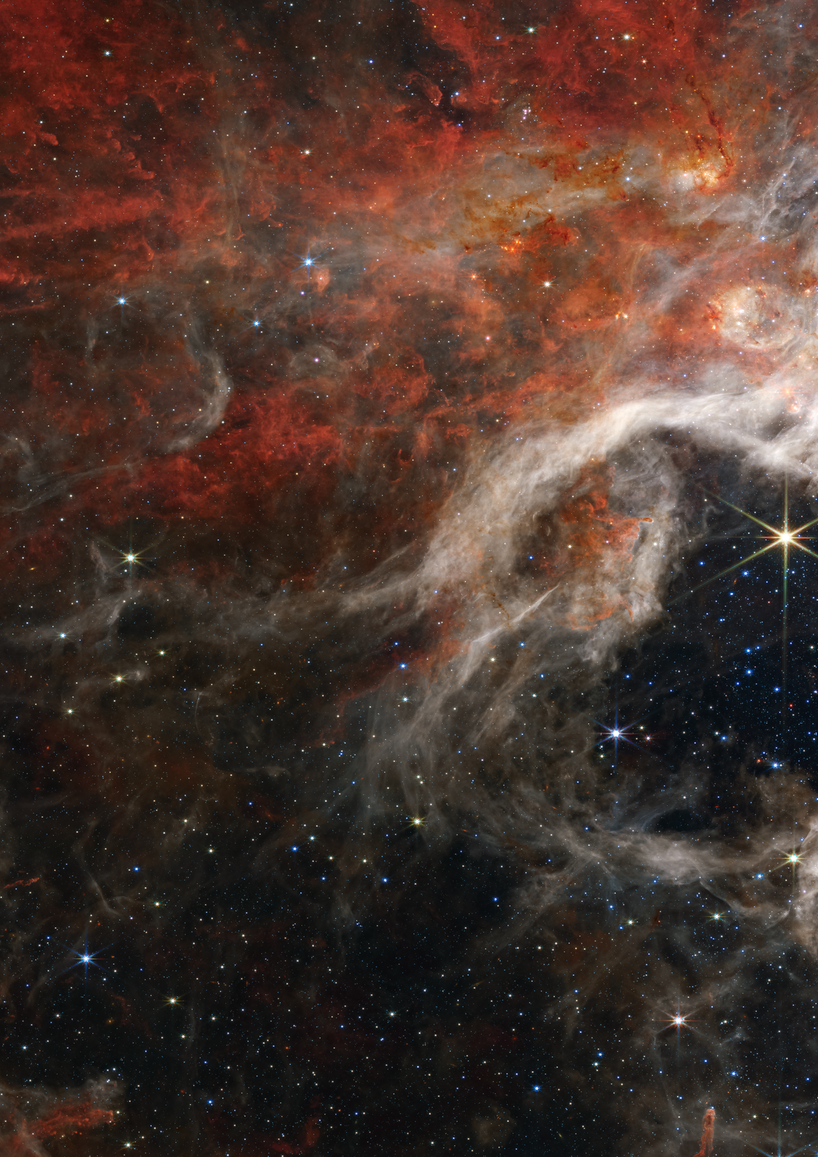
\includegraphics[width=\paperwidth]{Images/Tarantula_nebula1}}
    }
    \BgThispage
    
    \fancyfoot[C]{\color{white}\thepage}
%    \fancyfoot[L]{\vspace{3.5ex}\tiny\textcolor{white}{Credit: NASA, ESA, M. Livio, and the\\Hubble \nth{20} Anniversary Team (STScI)}}
    \fancyfoot[L]{\vspace{3.5ex}\tiny\textcolor{white}{Credit: NASA, ESA, CSA, STScI,\\JWST ERO Production Team}}
    \clearpage
    \newpage
    
    \renewcommand{\CurrentTitleColor}{\color{white}}
\fi

\chapter{Introduction}
\label{ch:Introduction}

\ifsetDraft
\else
    \renewcommand{\CurrentTitleColor}{\color{black}}
    
    \vspace*{\fill}
    \setlength{\epigraphwidth}{0.55\textwidth}
    {\color{white} \epigraph{\textit{Man muss noch Chaos in sich haben, um einen tanzenden Stern geb{\"a}ren zu k{\"o}nnen.}
        \\
        \vspace{2ex}
        \textit{You must have chaos within yourself to give birth to a dancing star.}}{--- Friedrich Nietzsche, Also sprach Zarathustra (1883)}}
    \vspace*{\fill}
    
    \backgroundsetup{
        scale=1,
        color=black,
        opacity=1,
        placement=top,
        angle=0,
        contents={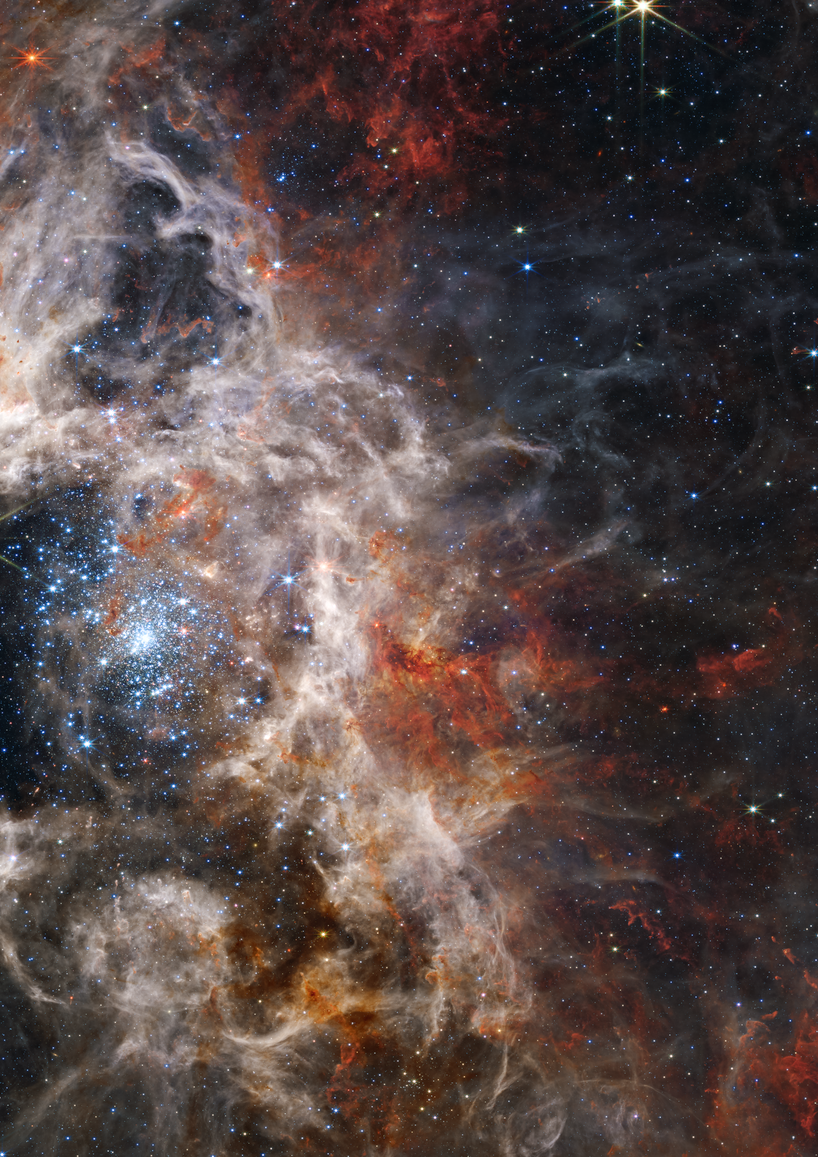
\includegraphics[width=\paperwidth]{Images/Tarantula_nebula2}}
    }
    \BgThispage
    
    \fancyhf{}
    \fancyfoot[C]{\color{white}\thepage}
    \newpage
    \setFancyHdr
\fi

%\addcontentsline{toc}{chapter}{Introduction}
%\chaptermark{Introduction}{}

%\renewcommand\thefigure{I.\arabic{figure}}
%\setcounter{figure}{0}

\section{Cosmological background}

\lettrine{M}{ankind} has long marvelled at the intricate structures of the Universe. Technological developments have enabled a more detailed view of the complexity seen in the night sky than ever, as exemplified by \textit{JWST} in \cref{chIfig:SMACS}. However, humanity has sought to explain the origin and evolution of the Universe long before the invention of the telescope. Indeed, the formulation of several key principles that underpin our current understanding of the Universe can be traced back to ancient times. Pythagoras is believed to be the first to describe the Universe as \textgreek{κόσμος} (cosmos), ancient Greek for ``order'', emphasising his attempt to capture the seemingly chaotic Universe as an orderly system \citep[e.g.][]{1860Humboldt}. Subsequent advances in the field of \textit{cosmology} were, and still are, enabled by standing on the shoulders of giants. For instance, based on the work of \citet{Copernicus1543} and others -- initiating a considerable philosophical paradigm shift in cosmology that removed the Earth from the centre of the cosmos -- \citet{Newton1687} not only introduced novel mathematical techniques to describe the physical world, but also conceived an important cosmological notion with his law of \textit{universal} gravitation, asserting the law applied uniformly throughout space. This, in turn, laid important groundwork for the developments that have led to the modern cosmological paradigm.
\begin{figure}
    \centering
    \includegraphics[width=\linewidth]{"Images/SMACS"}
    \caption[Colour composite image of the galaxy cluster SMACS 0723-73]
    {Colour composite image of the galaxy cluster SMACS 0723-73, taken by \textit{JWST}/NIRCam (programme ID 2736, PI: Pontoppidan) as part of the \textit{JWST} Early Release Observations \citep[EROs;][]{2022ApJ...936L..14P}. The multi-band imaging reveals a number of distant galaxies in the near-infrared (F444W in red, F356W in orange, F200W and F277W in green, F090W and F150W in blue). Credit: NASA, ESA, CSA, STScI.}
    \label{chIfig:SMACS}
\end{figure}

\subsection{Modern cosmology: theoretical and observational perspectives}
\label{chIssec:Modern_cosmology}

Founding the equivalence principle, \citet{1915SPAW.......844E} developed the theory of General Relativity (GR), relating the geometry of spacetime to the distribution of matter (or, equivalently, energy). However, it was realised soon after that GR can be applied as a theory of physical cosmology: a self-consistent mathematical description of the physical laws governing all matter across space and time, and indeed of the geometry of the spacetime continuum itself.\footnote{Note that a crucial assumption in these models is that the Universe is governed by the laws of GR: this implicitly assumes that gravity is the dominant force.} Modern cosmology is based on the \citeauthor{1915SPAW.......844E} field equation,
\begin{equation}
    \label{chIeq:Einstein_field_equation}
    R_{\mu \nu} - \frac{1}{2} g_{\mu \nu} R = \frac{8 \pi G}{c^4} T_{\mu \nu} \, ,
\end{equation}

\noindent where $R_{\mu \nu}$ is the Ricci tensor (defining the local curvature of spacetime), $g_{\mu \nu}$ is the metric (describing a local measure of time and distance), $R \equiv g^{\mu \nu} R_{\mu \nu}$ is the curvature scalar, $G$ is the gravitational constant, $c$ is the speed of light, and $T^{\mu \nu}$ is the energy-momentum tensor (encoding the matter content of the Universe).

\citet{1917SPAW.......142E} presented one of the first attempts at creating such a cosmological model within GR. Having realised that his theory only allowed for a contracting or expanding universe, Einstein introduced the concept of a cosmological constant $\Lambda$ (entering \cref{chIeq:Einstein_field_equation} as $\Lambda g_{\mu \nu}$) to contrive a static, but unstable, universe. Under the assumptions of homogeneity and isotropy collectively called the Cosmological Principle \citep{1933ZA......6....1M},\footnote{Equivalently, the Cosmological Principle states that the properties of the Universe appear the same to all observers; this is a generalisation of the Copernican Principle, which asserts that humans on Earth are not privileged observers.} a set of more general models of a universe governed by the laws of GR were independently constructed by \citet{1922ZPhy...10..377F} and \citet{1927PhDT.........6L}. These models describe a generic metric of curved spacetime containing a cosmological fluid with density $\rho$ and pressure $P$, which together form a solution to the field equations of GR.

Crucially, around the same time, it was found that in fact the Universe is not static, but expanding. Though many ``spiral nebulae'' had already been discovered \citep[e.g.][]{964AlSufi}, observations of Cepheid variables in these nebulae by \citet{1925ApJ....62..409H, 1926ApJ....63..236H} provided compelling evidence that they were themselves distant galaxies similar to the Milky Way, not diffuse gas clouds embedded within it. Then, \citet{1929PNAS...15..168H} reported that their recession velocity is proportional to their distance, $v = H_0 \, d$, an empirical relationship now known as Hubble's law. A uniformly expanding universe as predicted by the \citeauthor{1922ZPhy...10..377F} models provided an elegant explanation for this phenomenon. However, Einstein had not been alone in favouring the concept of a ``steady-state'' universe,\footnote{Famously, Einstein would later reportedly refer to the cosmological constant as ``the biggest blunder of my life''. Yet it may prove to be a fundamental constituent of our Universe, as will be discussed below.} since an expanding one brought about several uncomfortable ramifications. For instance, it implies that in the distant past, the Universe must have been increasingly denser and hotter, leading Fred Hoyle to scornfully coin the term \textit{Big Bang} for the hypothetical singularity at the beginning of time \citep[already considered by][]{1927PhDT.........6L}.\footnote{\citet{1961MNRAS.122..349R} presented evidence that was considered the final nail in the coffin of the steady-state theory that Fred Hoyle advocated, but the interdepartmental feud between the Cavendish Laboratory and the Institute of Astronomy would persist for some time.}

\subsection{Interlude: observers in an expanding universe}
\label{chIssec:Observers_in_an_expanding_universe}

Because of the Cosmological Principle, all of the time dependence in the spatial component of the metric can be parametrised by $a(t)$, the \textit{scale factor} of the universe. Specifically,
\begin{equation}
    \label{chIeq:FLRW_metric}
    \dif s^2 = c^2 \dif t^2 - a^2(t) \left[ \frac{\dif r^2}{1 - Kr^2} + r^2 \left( \dif \theta^2 + \sin^2 \theta \dif \phi^2 \right) \right] \, ,
\end{equation}

\noindent with cosmic time $t$, spatial coordinates $(r, \theta, \phi)$, and $K \in \{ -1, 0, 1 \}$ parametrising the curvature ($K = 0$ corresponds to a ``flat'' universe). Under a coordinate transformation $\dif \chi = \dif r / \sqrt{1 - Kr^2}$, a light ray following a null geodesic ($\dif s^2 = 0$) travels through an expanding universe on a radial trajectory (i.e. $\dif \theta = \dif \phi = 0$) that obeys
\begin{equation}
    \label{chIeq:Null_geodesic}
    \frac{\dif \chi}{\dif t} = \pm \frac{c}{a(t)} \, ,
\end{equation}

\noindent where $\chi$ is interpreted as the \textit{comoving} (radial) geodesic distance. In a flat universe, the coordinate $r$ takes the role of the radial geodesic, $\chi = r$, but note this does not generalise for $K \neq 0$. The physical separation between two points along the radial trajectory at a fixed time $t$, measured via \cref{chIeq:FLRW_metric}, is $\Delta l = a(t) \Delta \chi$.

In general, a particle's comoving coordinates, $\vec{\chi} = \vec{x} / a(t)$ with $\vec{x}$ being its proper (i.e. physical) coordinates, are constant in time if it is at rest. The scale factor is typically normalised to $a(t_0) = a_0 = 1$ at the present day so that comoving and proper coordinates coincide.\footnote{All quantities with subscript $0$ will refer to their present-day value (i.e. at $t = t_0$).} It is further customary to define the Hubble parameter $H(t) = \dot{a}/a$ (where the dot indicates a time derivative), with present-day value $H(t_0) = H_0$, the Hubble constant. For historical reasons, it is often parametrised as $h \equiv H_0/(100 \, \mathrm{km \, s^{-1} \, Mpc^{-1}})$.\footnote{This dimensionless $h$ is not to be confused with the Planck constant.} To understand its connection with the findings of \citet{1929PNAS...15..168H}, we consider the velocity of an object at coordinates $\vec{x}$,
\begin{equation}
    \label{chIeq:Hubbles_law}
    \vec{v} = \frac{\dif \vec{x}}{\dif t} = \frac{\dif a}{\dif t} \, \vec{\chi} + a(t) \, \frac{\dif \vec{\chi}}{\dif t} = \frac{\dot{a}}{a} \, \vec{x} + \vec{v}_\text{pec} \, ,
\end{equation}

\noindent where its \textit{peculiar velocity} is defined as $\vec{v}_\text{pec} \equiv a(t) \, \dif \vec{\chi} / \dif t$. This can be interpreted as the excess velocity of an object, its movement on top of the Hubble flow, $\vec{v}_\text{H} = H \, \vec{x}$, which instead is the perceived movement purely due to the expansion of the universe. If the object is at rest, $\vec{v}_\text{pec} = 0$, so that \cref{chIeq:Hubbles_law} evaluated at $t = t_0$ recovers Hubble's law.

Without going into the details, it can be shown \citep[see e.g.][]{2010gfe..book.....M} that the field equations of GR in a homogeneous and isotropic universe translate into the \citeauthor{1922ZPhy...10..377F} equations:
\begin{align}
    \label{chIeq:Friedmann_equation1}
    H^2 & = \frac{8 \pi G}{3} \rho - \frac{K c^2}{a^2} + \frac{\Lambda c^2}{3} \, ,
    \\
    \label{chIeq:Friedmann_equation2}
    \frac{\ddot{a}}{a} & =  -\frac{4 \pi G}{3} \left( \rho + \frac{3 P}{c^2} \right) + \frac{\Lambda c^2}{3} \, ,
\end{align}

\noindent where $\Lambda$ is a cosmological constant. The first law of thermodynamics (conservation of energy) within a volume $V$ requires
\begin{equation}
    \label{chIeq:First_law_thermodynamics}
    V \dif \rho + \left( \rho + \frac{P}{c^2} \right) \dif V = 0 \, ,
\end{equation}

\noindent so that given an equation of state $w \equiv P/\rho c^2$, the energy density $\rho_\text{x}$ of a specific type of matter evolves as
\begin{equation}
    \label{chIeq:Energy_density_scaling}
    \rho_\text{x} = \rho_{\text{x}, \, 0} \, \left( \frac{a}{a_0} \right)^{-3(1+w)} \, .
\end{equation}

Different types of energy content are characterised by the following equation of state: $w = 1/3$ for radiation or ultra-relativistic particles ($\rho_\text{r} \propto a^{-4}$; this implies the radiation temperature scales as $T_\text{r} \propto a^{-1}$, since $\rho_\text{r} \propto T_\text{r}^4$) and $w = 0$ for non-relativistic matter ($\rho_\text{m} \propto a^{-3}$). From \cref{chIeq:Friedmann_equation1,chIeq:Friedmann_equation2}, it can be seen that even a cosmological constant can be described as having a (non-evolving) energy density $\rho_\Lambda =\Lambda c^2/8 \pi G$ and $w = -1$. The energy density in a universe containing a mixture of these can then be written as
\begin{equation}
    \label{chIeq:Total_energy_density}
    \rho = \rho_\text{r} + \rho_\text{m} + \rho_\Lambda = \frac{\rho_{\text{r}, \, 0}}{a^4} + \frac{\rho_{\text{m}, \, 0}}{a^3} + \rho_{\Lambda, \, 0} \, .
\end{equation}

From this equation, it follows that the early Universe ($a \ll 1$) is radiation-dominated (i.e. $\rho \approx \rho_\text{r}$), then becomes matter-dominated (with matter-radiation equality when $\rho_\text{r} = \rho_\text{m}$), and finally becomes $\Lambda$-dominated. Having incorporated the cosmological constant in the energy density, it makes sense to define a critical density,
\begin{equation}
    \label{chIeq:Critical_density}
    \rho_\text{crit} \equiv \frac{3 H^2(t)}{8 \pi G} \, ,
\end{equation}

\noindent which, according to \cref{chIeq:Friedmann_equation1}, is the density (including a contribution of $\Lambda$) at which the curvature disappears, $K = 0$. Further defining the density parameter, $\Omega_\text{x} \equiv \rho_\text{x} / \rho_\text{crit}$, \cref{chIeq:Friedmann_equation1} can be rewritten as
\begin{align}
    \label{chIeq:Friedmann_equation1_alt1}
    H^2 & = \frac{8 \pi G}{3} \left( \frac{\rho_{\text{r}, \, 0}}{a^4} + \frac{\rho_{\text{m}, \, 0}}{a^3} + \rho_{\Lambda, \, 0} \right) - \frac{K c^2}{a^2} \nonumber
    \\
    & = H_0^2 \left( \frac{\rho_{\text{r}, \, 0}}{\rho_{\text{crit}, \, 0}} a^{-4} + \frac{\rho_{\text{m}, \, 0}}{\rho_{\text{crit}, \, 0}} a^{-3} + \frac{\rho_{\Lambda, \, 0}}{\rho_{\text{crit}, \, 0}} \right) - \frac{K c^2}{a^2} \nonumber
    \\
    & = H_0^2 \left( \Omega_{\text{r}, \, 0} a^{-4} + \Omega_{\text{m}, \, 0} a^{-3} + \Omega_{\Lambda, \, 0} \right) - \frac{K c^2}{a^2} \, ,
\end{align}

\noindent which specifies the evolution of the Hubble parameter in terms of the current-day density parameters, $\Omega_{\text{x}, \, 0} = 8 \pi G \rho_{\text{x}, \, 0} / 3 H_0^2$. Alternatively, dividing \cref{chIeq:Friedmann_equation1} by $H^2$ gives
\begin{equation}
    \label{chIeq:Friedmann_equation1_alt2}
    1 - \Omega = 1 - \Omega_\text{r} - \Omega_\text{m} - \Omega_\Lambda = - \frac{K c^2}{H^2 a^2} \, ,
\end{equation}

\noindent from which again it can be seen that $\rho = \rho_\text{crit}$ (i.e. $\Omega = \Omega_\text{r} + \Omega_\text{m} + \Omega_\Lambda = 1$) for a flat universe. As will be discussed in \cref{chIssec:LCDM_model}, it turns out our Universe appears to have $\Omega_0 \approx 1$: it has no (or very little) curvature. In a flat universe dominated by energy content of one type of matter (e.g. a radiation-dominated universe), the scale factor evolves as
\begin{equation}
    \label{chIeq:Scale_factor}
    a(t) \propto t^\frac{2}{3(1+w)} \, .
\end{equation}

An important concept related to the scale factor is the \textit{cosmological redshift} seen by a present-day observer. It is defined by
\begin{equation}
    \label{chIeq:Redshift}
    1 + z = \frac{a_0}{a(t)} \, ,
\end{equation}

\noindent such that $z = 0$ corresponds to the present. In an expanding universe, light emitted by a distant source at an early time $t_\text{emit}$ is redshifted, $\lambda_\text{obs} = (1 + z) \, \lambda_\text{emit}$, since the universe has expanded by a factor of $a_0 / a(t_\text{emit}) = (1 + z)$ between emission and observation. Combined with the finite speed of light that allows astronomers to effectively look back in time, observing the distant Universe as it was in the past, cosmological redshift is an important (though not physical) measure of distance to faraway sources.\footnote{Doppler shift due to peculiar motion along the line of sight can add an additional kinematic blueshift or redshift, but for the most distant sources this is a minor correction.}

\subsection{Concordance cosmology: the \texorpdfstring{\LCDM}{ΛCDM} model}
\label{chIssec:LCDM_model}

Following several other observational breakthroughs, the so-called \LCDM\ model has been established over the past few decades as our standard cosmological model. Dynamical measurements testing gravity on the scales of galaxies and galaxy clusters \citep{1933AcHPh...6..110Z, 1973A&A....26..483R, 1974Natur.250..309E, 1974ApJ...193L...1O, 1978ApJ...225L.107R, 1980ApJ...238..471R} first hinted at the existence of a non-baryonic mass component exhibiting only gravitational interaction.\footnote{In cosmology, baryons are simply defined as ``visible'' matter (i.e. massive particles susceptible to electromagnetic interactions); unlike in particle physics, this includes leptons.} \textit{Dark matter}, now hypothesised to be made up of massive, weakly interacting particles, gradually became an accepted paradigm. The study of distant supernova (SN) explosions furthermore led to the discovery of the accelerated expansion of the Universe \citep{1998AJ....116.1009R, 1998ApJ...507...46S, 1999ApJ...517..565P}, indicating the additional presence of \textit{dark energy}. As a more general version of Einstein's cosmological constant, dark energy causes spacetime to expand, which counteracts (and at the present epoch, even outweighs) gravitational contraction of the Universe.

The \LCDM\ model is thus named after these two main constituents: dark energy (specifically behaving like a cosmological constant $\Lambda$, i.e. $w = -1$) and cold dark matter (CDM).\footnote{The coldness refers to the thermal motions of the dark matter particles when they decouple, as will be discussed in \cref{chIsssec:Dark_matter_instabilities}.} The discovery of the cosmic microwave background \citep[CMB;][]{1965ApJ...142..419P, 1965ApJ...142..414D} allowed access to another powerful observational probe of cosmology, which has since firmly anchored the \LCDM\ paradigm.

First of all, the CMB provides strong evidence for the Big Bang theory as it nearly perfectly resembles blackbody emission (cf. \cref{chIssec:Effects_of_dust}), observed today at $T_{\text{CMB}, \, 0} = 2.725 \, \mathrm{K}$ \citep[e.g.][]{2009ApJ...707..916F}, proving the early Universe was hot and dense \citep[in fact, the existence of the CMB in a Big Bang model had been predicted before its discovery;][]{1949RvMP...21..367G}. After this hot, ionised plasma in the early Universe had cooled down sufficiently due to expansion, protons and electrons were able to recombine \citep[at a redshift of $z \sim \num{1100}$; e.g.][]{1985A&A...149..144J}.\footnote{Note that this terminology is misleading, since the epoch of recombination was the very first time that stable, neutral atoms were able to form.} The sudden phase transition turned the hot plasma into neutral gas that was no longer opaque, releasing the (henceforth) ever-present relic radiation. Furthermore, the extremely high degree of isotropy seen in the CMB, with fluctuations of the order of $\delta T / T \sim 10^{-5}$, makes a compelling case for the validity of the Cosmological Principle, while the angular power spectrum of precisely these fluctuations is described remarkably well by \LCDM\ \citep{2020A&A...641A...1P}. Detailed fitting procedures provide high-precision measurements of its six free parameters. The latest results \citep[e.g.][]{2020A&A...641A...6P} show that:
\begin{enumerate}[label=(\roman*)]
    \item the current expansion rate of the Universe, as measured through the Hubble constant, is $H_0 = 67.4 \pm 0.5 \, \mathrm{km \, s^{-1} \, Mpc^{-1}}$;
    \item dark matter significantly dominates over baryonic matter, which only makes up around one sixth of the matter content ($\Omega_{\text{b}, \, 0} \sim 0.05$, while $\Omega_{\text{m}, \, 0} \sim 0.3$);
    \item dark energy currently trumps matter ($\Omega_{\Lambda, \, 0} \sim 0.7$) and is consistent with a cosmological constant (i.e. equation of state $w = -1$);
    \item the total density appears to be close to the critical density ($\Omega_0 = 1$), which implies the Universe is spatially flat.
\end{enumerate}

Unless explicitly mentioned otherwise (in particular in \cref{ch:Prospects_for_observing_the_low-density_cosmic_web_in_Lya_emission}), I assume $\Omega_{\text{m}, \, 0} = 0.3$, $\Omega_{\Lambda, \, 0} = 0.7$, and $H_0 = 70 \, \mathrm{km \, s^{-1} \, Mpc^{-1}}$ (i.e. $h = 0.7$) throughout to ease comparison with previous studies.

\subsection{Structure formation in a homogeneous and isotropic universe}
\label{chIssec:Structure_formation_in_a_homogeneous_and_isotropic_universe}

Despite the success of the \LCDM\ model in reproducing the statistical properties of the CMB, several conceptual problems remain. How can a homogeneous and isotropic model universe, adhering to the assumptions of the Cosmological Principle, ever achieve the observed complexity such as that shown in \cref{chIfig:SMACS}? This issue can be resolved by considering the model as an approximation that becomes valid at sufficiently large scales, $l \gtrsim 200 \, \mathrm{cMpc}$ (where $\mathrm{cMpc}$ denotes a comoving megaparsec) according to simulations \citep[e.g.][]{2010MNRAS.405.2009Y}. Indeed, a strictly homogeneous universe would not see the formation of any structure; such a model universe devoid of galaxies, stars, and planets is evidently not a representative model for the observed Universe. This statement may seem obvious, but it underlines the effectiveness of the relatively simple \LCDM\ model at explaining the formation of complex cosmological structures as local deviations from a homogeneous background.

Another challenge facing the \LCDM\ model, then, are the initial conditions, which need to be understood in order to make useful predictions about the cosmic structure observed today. As first shown by \citet{1970PhRvD...1.2726H} and \citet{1972MNRAS.160P...1Z}, galaxy-sized structures can be formed by \textit{primordial} fluctuations (i.e. perturbations that are in place at very early times) only if these take the form of a scale-invariant power spectrum. A pure GR description of the Universe, however, encounters more problems at very early times, particularly when typical scales in the universe approached the Planck scale ($m_\text{P} \sim 10^{19} \, \mathrm{GeV}/c^2$). On larger scales, gravity is assumed to dominate over the electromagnetic, strong, and weak interactions but at sufficiently small scales these forces start to compete with gravity, requiring a theory of quantum gravity to be properly understood.\footnote{A quantum description of matter does not have a definitive spatial distribution (let alone true homogeneity), which makes a reconciliation of quantum theory and GR difficult.} Certainly, in the so-called Planck epoch -- the first $t_\text{P} \sim 10^{-43} \, \mathrm{s}$ after the Big Bang -- the basic \LCDM\ model is no longer valid. Further problems arise from interpreting observations of the CMB: its isotropy suggests polar-opposite regions, despite not having been in causal contact, were somehow at (nearly perfect) thermal equilibrium when the CMB was released \citep[the ``horizon problem'';][]{1968ApJ...151..431M}. Moreover, the spatial flatness observed today requires extreme fine-tuning of the initial curvature of the Universe \citep[the ``flatness problem'';][]{1979grec.conf..504D}.

It turns out that a solution for the latter two problems, namely extending the \LCDM\ model with a brief period of exponential expansion (\textit{inflation}) shortly after the Big Bang, also alleviates the issue of not (yet) having a unifying theory valid at extremely high energies \citep{1980PhLB...91...99S, 1980ApJ...241L..59K, 1981PhRvD..23..347G, 1982PhLB..108..389L, 1982PhRvL..48.1220A}. Without having to specify the exact physical properties of the Universe at the Planck epoch, the quantum fluctuations of the scalar field driving inflation (with corresponding particle called the \textit{inflaton}) simultaneously provide a natural explanation for a nearly scale-invariant Gaussian random field of initial density perturbations \citep{1982PhLB..115..295H, 1982PhRvL..49.1110G, 1983PhRvD..28..679B}.

Although several modifications and/or replacements have been proposed,\footnote{There exists observational evidence that further extensions of the \LCDM\ model may be required. There are, for instance, hints of cosmic anisotropy \citep[e.g.][]{2022arXiv220805018P} and the Hubble constant determined from the CMB deviates from local measurements \citep{2020A&A...641A...6P}. Other tension, such as the ``cusp-core'' and ``missing-satellite'' problems are generally attributed to the detailed effects of galaxy formation \citep[``baryonic physics''; e.g.][]{2012MNRAS.421.3464P, 2016ApJ...827L..23W}.} the \LCDM\ model (coupled to inflation) is unrivalled in its ability to accurately explain and quantitatively reproduce a plethora of statistical properties of observed cosmic structure. It offers a comprehensive explanation for the formation and evolution of structure seen across more than $\ssim 99.997\%$ of cosmic time, from the highly isotropic CMB to today's diverse population of galaxies embedded in a complex cosmic network, as depicted in \cref{chIfig:Cosmic_timeline}. The next section will go into the details of the formation and evolution of these galaxies in a \LCDM\ universe.

\section{Galaxy formation and evolution: a brief history of time}

In the \LCDM\ model, structures of visible matter, such as galaxies, form in hierarchical manner on top of a dark matter firmament, all having grown from inflated quantum fluctuations. The following sections will discuss the various assembly stages of these structures (shown schematically in \cref{chIfig:Cosmic_timeline} as a timeline of the Universe) as well as the polluting and destructive impact of galaxies on their environment, in the form of chemical enrichment and ionising radiation. Shortly after the Big Bang, inflation sets the initial conditions for the formation of structure, which can be probed via the CMB (discussed in \cref{chIssec:Inflation_until_CMB}). Density fluctuations grow throughout the dark ages (\cref{chIssec:Growth_of_structure_in_the_linear_regime,chIssec:Non-linear_collapse}), resulting in the formation of the first stars and galaxies at \textit{cosmic dawn} (\cref{chIssec:Galaxy_formation}). The onset of star formation (\cref{chIssec:Star_formation_and_stellar_evolution}), in turn, initiated the creation of the first heavy elements (\cref{chIssec:Chemical_enrichment}) and led to the reionisation of the Universe (\cref{chIssec:Epoch_of_Reionisation}). However, all good things come to an end and at present, we find ourselves in an epoch of declining star formation activity (\cref{chIssec:Cosmic_noon_and_the_epoch_of_quenching}).
\begin{figure}[t]
    \centering
    \includegraphics[width=\linewidth]{"Images/NAOJ_timeline_highres"}
    \caption[Schematic timeline of the Universe]
    {Schematic timeline of the Universe. Time increases from left to right, indicated on top, redshift as defined in \cref{chIeq:Redshift} increases from right to left on the bottom (note neither of these scales are linear). Several important evolutionary stages of the early Universe are indicated, focussing on Cosmic Reionisation (\cref{chIssec:Epoch_of_Reionisation}). Credit: NAOJ.}
    \label{chIfig:Cosmic_timeline}
\end{figure}

\subsection{Inflation until the CMB: synthesis of the first elements}
\label{chIssec:Inflation_until_CMB}

Towards the end of inflation, the release of the potential energy of the inflaton field (\textit{reheating}) leaves the Universe in a hot and dense state \citep[ultimately the source of the blackbody nature of the CMB;][]{1994PhRvL..73.3195K}. Quantum fluctuations of the inflaton field cause a (nearly) scale-invariant Gaussian random field of density perturbations to be imprinted on the density field, as described above. Within a fraction of a second after the Big Bang, the Universe expands and cools down sufficiently to enter the realm of the Standard Model of particle physics ($T \lesssim 10^{15} \, \mathrm{K}$ or $E \lesssim 150 \, \mathrm{GeV}$) and to now be filled with a quark-gluon plasma. Still within the first second of cosmic time, quarks are able to settle into hadrons, including protons and neutrons.

Importantly, interactions between protons and neutrons began to allow atomic nuclei heavier than hydrogen (i.e. a proton) to form in a process called Big Bang Nucleosynthesis \citep[BBN; work on this was pioneered by][]{1949RvMP...21..367G}. However, requiring a temperature that is low compared to the binding energy of a nucleus means that the density was no longer high enough for (a sufficiently high interaction rate of) many-body collisions, so that only the lightest elements (He, Li) can form at appreciable abundances \citep{1967ApJ...148....3W}.\footnote{The chemical network of two-body reactions is not able to go beyond lithium due to a lack of stable nuclei with atomic weight of 5 or 8 \citep[e.g.][]{2010gfe..book.....M}. The origin of heavier elements will be discussed in \cref{chIssec:Chemical_enrichment}.} As a result, primordial nucleosynthesis is predicted to yield a $\ssim 25\%$ mass fraction of helium, in excellent agreement with observations \citep[and hence considered a key validation of the Big Bang theory;][]{2016RvMP...88a5004C}.

As the Universe expands and cools down further, species start to \textit{decouple} from the primordial plasma, meaning they fall out of thermal equilibrium. At $z \sim 3400$, the energy densities of relativistic and non-relativistic particles (i.e. radiation and matter, respectively) become equal and the Universe enters the matter-dominated phase. As discussed above, CMB photons are released as matter and radiation decouple at $z_\text{dec} \sim 1100$, or about $\num{380000} \, \mathrm{yr}$ after the Big Bang \citep{2010gfe..book.....M}. This signified the beginning of the cosmic \textit{dark ages} (see \cref{chIfig:Cosmic_timeline}).

\subsection{Dark ages: growth of structure in the linear regime}
\label{chIssec:Growth_of_structure_in_the_linear_regime}

Ironically, radiation freely roamed the Universe for the first time during the dark ages, but they would have been truly dark to the human eye: CMB photons were redshifting away from visible wavelengths while there were no other optical light sources (causing the dark ages to appear rather uninteresting in \cref{chIfig:Cosmic_timeline}). Directly observing the dark ages, however, may in theory be achieved through the 21-cm line emitted by neutral hydrogen \citep[e.g.][]{2006PhR...433..181F}. Furthermore, like their historical counterpart, the fact that there is no clear record of what exactly happened does not make the dark ages any less eventful: primordial density fluctuations would steadily grow -- in fact, dark matter perturbations were already enhanced, as will be discussed in \cref{chIsssec:Dark_matter_instabilities} -- soon leading to the formation of the astrophysical objects.

As first shown by \citet{1902RSPTA.199....1J}, gravitational instability allows perturbations to grow into evolved structures provided their size exceeds a critical threshold, below which internal pressure prevents collapse. The \citeauthor{1902RSPTA.199....1J} formalism considers the linear regime of perturbations in the density field $\rho$, $\delta \equiv (\rho - \bar{\rho}) / \bar{\rho}$ with $\delta \ll 1$, against a background of constant density, $\bar{\rho}$. In the Newtonian description of a non-relativistic fluid in an expanding universe, the perturbations, decomposed the into Fourier modes (with comoving wavenumber $k = 2\pi a(t) / \lambda$), can be shown to satisfy
\begin{equation}
    \label{chIeq:Jeans_instability}
    \ddot{\delta}_k + 2 H \dot{\delta}_k + \left( \frac{c_\text{s}^2 k^2}{a^2} - 4 \pi G \bar{\rho} \right) \delta_k = 0 \, ,
\end{equation}

\noindent where $c_\text{s}$ is the adiabatic speed of sound. This describes a damped harmonic oscillator with angular frequency $\omega_k$ satisfying $\omega_k^2 = \frac{c_\text{s}^2 k^2}{a^2} - 4 \pi G \bar{\rho}$. The \citeauthor{1902RSPTA.199....1J} length, a critical scale for which $\omega_k^2 = 0$, is given in proper units by
\begin{equation}
    \label{chIeq:Jeans_length}
    \lambda_\text{J} = c_\text{s} \sqrt{\frac{\pi}{G \bar{\rho}}} \, ,
\end{equation}

\noindent with corresponding \citeauthor{1902RSPTA.199....1J} mass enclosed by a sphere of diameter $\lambda_\text{J}$,
\begin{equation}
    \label{chIeq:Jeans_mass}
    M_\text{J} = \frac{4}{3} \pi \bar{\rho} \left( \frac{\lambda_\text{J}}{2} \right)^3 = \frac{\pi}{6} \bar{\rho} \lambda_\text{J}^3 \, .
\end{equation}

Modes below the critical scale, $\lambda \ll \lambda_\text{J}$, act as acoustic waves, oscillating around hydrostatic equilibrium where pressure counteracts gravity. On the other hand, gravity is able to overcome the internal pressure support for perturbations satisfying the criterion for collapse, $\lambda \gg \lambda_\text{J}$. In this case, $\omega_k$ is imaginary and the equation describes a (stationary) growing or decaying mode instead. In both cases, the universe's expansion offers additional support against gravitational collapse -- the ``Hubble drag'' -- causing a damping of the acoustic waves and a slowing in the growth (or decay) of an instability.

\subsubsection{Baryonic instabilities}
\label{chIsssec:Baryonic_instabilities}

When radiation and baryons are still coupled, radiation pressure is sufficiently high to prevent the collapse of all but the largest structures, corresponding to $M_\text{J} \sim 10^{16} \, \mathrm{M_\odot}$ \citep[the mass of the largest galaxy clusters;][]{2010gfe..book.....M}. Formally, the \citeauthor{1902RSPTA.199....1J} analysis needs be extended to include relativistic effects \citep[e.g.][]{1946ZhETF..16..587L} as the assumption of a non-relativistic background fluid no longer holds in the radiation-dominated phase, but the result is qualitatively the same. As a consequence, perturbations of the photon-baryon plasma in the pre-recombination era drive baryon acoustic oscillations (BAO), whose imprint can be seen in the CMB.

Another consequence of relativistic effects is a distinction between the growth of modes within and beyond than the (comoving) particle horizon at a given time $t$,
\begin{equation}
    \label{chIeq:Particle_horizon}
    \chi_\text{h}(t) = \int_{0}^{t} \frac{c \dif t'}{a(t')} \, ,
\end{equation}

\noindent which is interpreted as the radius beyond which light rays information cannot have reached the origin (cf. \cref{chIeq:Null_geodesic}). It increases with time, at least in the radiation- and matter-dominated eras; modes therefore only start to grow once they have entered the horizon, while super-horizon modes are ``frozen''. Before recombination, all sub-horizon modes of baryonic perturbations fall below the \citeauthor{1902RSPTA.199....1J} scale so that each mode entering the horizon assumes oscillatory behaviour \citep[e.g.][]{1981ApJ...248..885P}.

Recombination then marks a sharp phase transition where free electrons were rapidly captured, although this was not quite an instantaneous process. There was a brief period where the mean free path (MFP) of photons was some finite value, in contrast to the earlier radiation-dominated phase and the later dark ages where, relative to scales $\lambda_\text{g}$ relevant for galaxy formation, the MFP was effectively zero ($\lambda_\text{MFP} \ll \lambda_\text{g}$) and infinity ($\lambda_\text{MFP} \gg \lambda_\text{g}$), respectively \citep{1968ApJ...151..459S}. As a result, photons preferentially diffuse from overdense into underdense regions, the so-called \citeauthor{1968ApJ...151..459S} damping, thereby smoothing out small-scale perturbations below the damping scale of $M_\text{d} \sim 10^{14} \, \mathrm{M_\odot}$. Considering baryonic fluctuations alone therefore suggests galaxy formation occurs in a top-down scenario, requiring the surviving large perturbations to fragment into smaller, galaxy-sized ($M \sim 10^{11} \, \mathrm{M_\odot}$) structures (in disagreement with observations).

After decoupling, radiative pressure support falls away and is replaced by gas pressure. At this stage, baryons can be described well by an ideal, non-relativistic, monoatomic gas at temperature $T$, so that
\begin{equation}
    \label{chIeq:Ideal_gas}
    c_\text{s} = \frac{5}{3} \frac{k_\text{B} T}{m_\text{p}} \, ,
\end{equation}

\noindent where $k_\text{B}$ is the Boltzmann constant and $m_\text{p}$ is the proton mass. This results in a much-reduced \citeauthor{1902RSPTA.199....1J} mass approximately equal to the size of a globular cluster, $M_\text{J} \sim 10^{6} \, \mathrm{M_\odot}$, suggesting structure on galactic scales start to collapse at this point \citep{2010gfe..book.....M}. Indeed, it can be shown that for a pressureless fluid (or equivalently for sufficiently large modes, $\lambda \gg \lambda_\text{J}$) the growing mode in the matter-dominated regime scales (almost) linearly with the scale factor, $\delta \appropto a \propto (1+z)^{-1}$ \citep{1992ARA&A..30..499C}.
\begin{figure}
    \centering
    \includegraphics[width=\linewidth]{"Figs/Neutral_gas_distribution"}
    \caption[Simulated column density of neutral hydrogen at $z = 7$]
    {Simulated column density of neutral hydrogen, $N_\text{\ion{H}{I}}$, at $z = 7$. The neutral hydrogen distribution in the cosmological hydrodynamical simulation (cf. \cref{ch:Prospects_for_observing_the_low-density_cosmic_web_in_Lya_emission}) is shown for the full extent of the simulation box, $40 \times 40 \, h^{-2} \, \mathrm{cMpc}^2$, for a $\ssim 5.5 \, h^{-1} \, \mathrm{cMpc}$ depth. Baryonic matter closely follows the underlying dark matter distribution, without which fluctuations seen in the CMB could not have grown into the structures observed today, as discussed in \cref{chIsssec:Baryonic_instabilities,chIsssec:Dark_matter_instabilities}. The cosmological density field (here traced via neutral hydrogen) reveals a complex, web-like structure with large voids and overdense regions.}
    \label{chIfig:Neutral_gas_distribution}
\end{figure}

The relatively slow growth rate combined with the effect of \citeauthor{1968ApJ...151..459S} damping, however, requires large initial fluctuations to form observed clusters of galaxies (with masses comparable to the damping scale, $M \gtrsim 10^{14} \, \mathrm{M_\odot}$). If these structures are seeded by initial perturbations in the baryonic density field, and the onset of growth occurs at decoupling, $z_\text{dec} \sim 1100$, the observed temperature fluctuations in the CMB\footnote{Perturbations in the radiation temperature, $\delta T$, are related to those in matter density, $\delta$, as $\delta T / T = \delta/3$, since $T_\text{r} \propto \rho_\text{m}^{1/3}$ (this can be seen from the scaling relations $T_\text{r} \propto a^{-1}$ and $\rho_\text{m} \propto a^{-3}$).} would need to be of the order of $\delta T / T \sim 10^{-3}$ to reach $\delta \sim 1$ (where non-linear structure forms; \cref{chIssec:Non-linear_collapse}) at $z = 0$, two orders of magnitude larger than what is observed. The severe mismatch between purely baryonic cosmological models of galaxy formation and the observed Universe provides further key evidence for the existence of a significant dark matter component, which can remedy these issues.

\subsubsection{Dark matter instabilities}
\label{chIsssec:Dark_matter_instabilities}

Dark-matter perturbations undergo a substantially different evolution compared to the baryonic behaviour discussed above, since dark matter had decoupled at very early times owing to its weak electromagnetic interaction. In the radiation-dominated regime, dark matter (sub-horizon) perturbations can already slowly grow, scaling logarithmically with the scale factor.\footnote{With the exception that for prevailing non-relativistic perturbations in a background density dominated by a relativistic component (i.e. $\bar{\rho}_\text{r} \delta_\text{r} \ll \bar{\rho}_\text{dm} \delta_\text{dm}$ in the radiation-dominated phase), as is the case for dark matter perturbations approaching the time of matter-radiation equality, the growing mode actually stagnates due to the Hubble drag \citep{1974A&A....37..225M}.}

Most importantly, however, the dark matter instabilities start to grow at near-linear pace from the matter-radiation equality onwards \citep{1992ARA&A..30..499C}, allowing them to get ahead of the baryonic perturbations that are trapped in acoustic waves until recombination. With the radiation field having been critically diluted after the matter-radiation equality, dark matter effectively becomes the Universe's main constituent, while baryons only serve a subdominant role making up one sixth of the matter content (\cref{chIssec:LCDM_model}). After recombination, baryons therefore quickly fall into the strong gravitational potential wells of dark matter overdensities, circumventing the effects of \citeauthor{1968ApJ...151..459S} damping by which dark matter is not affected, since it had decoupled long before recombination.

However, dark matter still suffers from \textit{free streaming}: initial velocities, imposed by thermal equilibrium in the primordial plasma, also have a smoothing effect on small-scale density enhancements. Equivalently, the \citeauthor{1902RSPTA.199....1J} formalism can still be applied to the collisionless dark matter if the adiabatic speed of sound $c_\text{s}$ in \cref{chIeq:Jeans_length} is replaced by its velocity dispersion $\sigma_\text{dm}$, which acts effectively as a pressure on small scales. Less massive dark matter particles have higher velocities when they decouple, which washes out small-scale density perturbations. A characteristic particle mass of $m_\text{g} \sim 1 \, \mathrm{keV}/c^2$ leads to perturbations being affected at (and below) typical galactic scales, making the case for CDM ($m \gg m_\text{g}$) as opposed to warm ($m \sim m_\text{g}$) or hot ($m \ll m_\text{g}$) dark matter cosmologies \citep[e.g.][]{1982ApJ...263L...1P}.

To illustrate the growth of structure in the ($\Lambda$)CDM paradigm, the simulated neutral hydrogen column density, $N_\text{\ion{H}{I}}$,\footnote{Here, \ion{H}{I} is the spectroscopic notation for neutral hydrogen; see \cref{chIssec:Definitions_and_notation} for details.} of a large cosmological volume at $z = 7$ is shown in \cref{chIfig:Neutral_gas_distribution}. The specific cosmological simulation used to produce this neutral hydrogen distribution will be described in detail in \cref{ch:Prospects_for_observing_the_low-density_cosmic_web_in_Lya_emission} (see \cref{appPfig:NHI} in particular). The displayed area is equal to the full simulation box extent, $40 \times 40 \, h^{-2} \, \mathrm{cMpc}^2$, over a depth of $\ssim 5.5 \, h^{-1} \, \mathrm{cMpc}$ (which would correspond to a \lymana\ narrowband image with $\Delta \lambda_\text{obs} = 17.5 \, \Angstrom$; cf. \cref{chPsssec:Narrowband}). The cosmological density field, here traced via neutral hydrogen, reveals a complex, web-like structure called the \textit{cosmic web} at scales above approximately a few $\mathrm{cMpc}$ (though it starts to appear homogeneous at $l \gg 200 \, \mathrm{cMpc}$, as discussed in \cref{chIssec:Structure_formation_in_a_homogeneous_and_isotropic_universe}; see also \cref{ch:Prospects_for_observing_the_low-density_cosmic_web_in_Lya_emission}).

The precise appearance of the cosmic web is a result of the hierarchical formation of structure: small structures form first, merging into increasingly larger objects. Though directly observing the cosmic web is extremely challenging, since the bulk of baryonic matter hardly emits any light, efforts are underway to do precisely this, as will be discussed in \cref{ch:Prospects_for_observing_the_low-density_cosmic_web_in_Lya_emission}. The density field can be probed indirectly, however, via the large-scale distribution of galaxies, with the $\Lambda$CDM model predicting each galaxy is placed at the centre of a \textit{dark matter halo}. To understand the next stages in the process of galaxy formation, taking place at scales orders of magnitude smaller than that of the cosmic web shown in \cref{chIfig:Neutral_gas_distribution}, linear theory does not suffice any more: once $\delta \sim 1$, non-linear effects start to play a role as the perturbation itself becomes more important than the homogeneous background. Overdense regions can decouple from the Hubble flow and (in the case of dark matter) establish a dynamical quasi-equilibrium.

\subsection{Non-linear gravitational collapse}
\label{chIssec:Non-linear_collapse}

In the non-linear regime, analytical solutions for gravitational collapse are only available for special cases, for instance if spherical symmetry of the system is assumed \citep[e.g.][]{1972ApJ...176....1G}. These idealised models still provide useful insights into the complex dynamical process of gravitational instability, however, indicating a runaway, non-linear collapse sets in at an overdensity of $\delta \approx 1.686$. However, once a region exceeds this threshold it will not, in general, collapse down to a point mass (as is evident from galaxies abundantly visible today),\footnote{Though it is speculated that supermassive black holes ($M_\text{BH} \gtrsim 10^5 \, \mathrm{M_\odot}$) may form as a result of direct collapse in the early Universe \citep[e.g.][]{2003ApJ...596...34B}.} but rather settle into a quasi-equilibrium upheld by random motions.

Structures formed by collapsing dark matter overdensities are called dark matter halos, prevented from collapsing further by their velocity dispersion: the system gradually relaxes into \textit{virial equilibrium}, a state in which the gravitational potential energy and the kinetic energy of the collisionless dark matter particles are balanced. Galaxies, containing large numbers of stars travelling in virtually empty space, can also be considered collisionless dynamical systems. Detailed analyses show that virialised structures end up at a density contrast relative to the background density of approximately $\Delta_\text{vir} \equiv \delta (t_\text{vir}) \sim 200$ \citep{1998ApJ...495...80B}.

If a dark matter halo has reached virial equilibrium, this density contrast can be used to relate its virial mass and radius,
\begin{equation}
    \label{chIeq:Virial_mass}
    M_\text{vir} = \frac{4}{3} \pi R_\text{vir}^3 \Delta_\text{vir} \bar{\rho} \, .
\end{equation}

Inversely, $\Delta_\text{vir}$ can be fixed a priori (often $\Delta_\text{vir} = 200$) to specify the masses and radii of dark matter halos in cosmological simulations, assuming they are virialised (as will be done in \cref{ch:Prospects_for_observing_the_low-density_cosmic_web_in_Lya_emission}). Dark matter halos hosting galaxies typically have $10^{10} \, \mathrm{M_\odot} \lesssim M_\text{vir} \lesssim 10^{14} \, \mathrm{M_\odot}$ and virial radii ranging from several tens to hundreds of kiloparsecs. For instance, a typical spiral galaxy in the local Universe with stellar mass of the order of $M_* \sim 10^{11} \, \mathrm{M_\odot}$ -- the Milky Way is thought to be a good example -- will be embedded in a $\ssim 10^{12} \, \mathrm{M_\odot}$ dark matter halo with a virial radius of the order of $R_\text{vir} \sim 200 \, \mathrm{kpc}$ \citep[e.g.][]{2013ApJ...764L..31K}. Another important quantity is $T_\text{vir}$, the virial temperature, defined as
\begin{equation}
    \label{chIeq:Virial_temperature}
    k_\text{B} T_\text{vir} = \frac{1}{2} m v_\text{vir}^2 = \frac{G m M_\text{vir}}{2 R_\text{vir}} \, ,
\end{equation}

\noindent where $m$ is the particle mass and the virial velocity $v_\text{vir}$ is simply taken to be the circular velocity at the virial radius, $v_\text{vir}^2 = G M_\text{vir} / R_\text{vir}$. The particle mass can be written as $m = \mu m_\text{p}$, where $\mu$ is the mean molecular weight and $m_\text{p}$ is the proton mass; for instance, $m \simeq 0.59 m_\text{p}$ for a fully ionised, primordial gas (consisting of hydrogen and helium at primordial abundances). For a typical galaxy-sized halo, this results in a virial temperature of the order of $10^6 \, \mathrm{K}$ \citep[where, to good approximation, a primordial gas indeed is fully ionised; e.g.][]{2010gfe..book.....M}.

Combining the linear and non-linear regimes, \citet{1974ApJ...187..425P} developed an analytical method that predicts the mass function of dark matter halos over cosmic time assuming initial Gaussian random fluctuations. Evolving the Gaussian field over time according to the regime of linear growth, the method presents a way to compute the number density of fluctuations having exceeded the threshold for non-linear collapse ($\delta \approx 1.686$) which are sufficiently large to form a given mass, assuming that all these have formed virialised dark matter halos. The resulting mass function is a power-law for low-mass halos with an exponential cut-off beyond a characteristic mass that grows over time, reflecting the hierarchical formation process. This simple framework proved a fairly good model for the observed Universe (at least qualitatively), as evidenced by the galaxy luminosity function which is typically described well by the same type of function \citep[][]{1976ApJ...203..297S}. More accurate halo mass functions can be obtained using cosmological $N$-body simulations \citep[e.g.][]{2008ApJ...688..709T}.

Having discussed the formation and main properties of dark matter halos, the next section will focus on the processes involved in the formation of galaxies at the centres of these dark matter halos.

\subsection{First light: dawn of the first stars and galaxies}
\label{chIssec:Galaxy_formation}

In the local Universe, galaxies typically have sizes (as measured through their stellar light distribution) of the order of $10 \, \mathrm{kpc}$ and below, while their dark matter halo, as discussed above, extends to much larger radii. If virial equilibrium prevents further gravitational collapse, then how are galaxies able to form in the first place? The answer to this question lies in radiative dissipation: unlike dark matter, baryons are able to radiate away excess energy through various mechanisms, thereby ridding itself of gravitational potential energy. In the right mass regime, cooling allows gas to condense at the centre of dark matter halos and hence is an essential ingredient of galaxy formation \citep{1977ApJ...211..638S, 1977MNRAS.179..541R, 1977ApJ...215..483B, 1978MNRAS.183..341W}.

When baryons fall into the potential wells of dark matter halos that establish after recombination (\cref{chIsssec:Dark_matter_instabilities}), gas would, in the absence of cooling, be shock-heated to the virial temperature upon reaching the virial radius, establishing a hydrostatic equilibrium that prevents further collapse. Provided the cooling process is efficient, however, gas is able to contract further (the ``cold mode'' of gas accretion), though it retains its angular momentum since the emission is isotropic. In this case, a flattened, rotating, gaseous disc, fed by smooth accretion of cold gas, forms at the centre of the potential well.\footnote{For the most massive halos, $M \gtrsim 10^{11} \, \mathrm{M_\odot}$, cooling is inefficient (as discussed in \cref{chIsssec:Dissipative_processes}) and a stable shock front forms \citep[``hot-mode'' accretion;][]{2003MNRAS.345..349B}. This mainly becomes important at later times ($z \lesssim 2$; see also \cref{chIssec:Cosmic_noon_and_the_epoch_of_quenching}).} Within the disc, gas is able to fragment further and is converted into stars (discussed in further detail in \cref{chIssec:Star_formation_and_stellar_evolution}).

\subsubsection{Dissipative processes}
\label{chIsssec:Dissipative_processes}

The cooling efficiency is determined by the composition, density, and temperature of the gas. It can be quantified by comparing the cooling timescale, $t_\text{cool} \propto T/\Lambda(T)$ (where $\Lambda(T)$ is the cooling function, which depends on the gas metallicity; see \cref{chIssec:Chemical_enrichment}), to the free-fall timescale, $t_\text{ff} \propto 1/\sqrt{G\rho}$, which indicates how long gravitational collapse would take in the absence of internal pressure support.

The most efficient cooling (where $t_\text{cool} \ll t_\text{ff}$) occurs through collisional excitation at gas temperatures of $10^4 \, \mathrm{K} \lesssim T \lesssim 10^6 \, \mathrm{K}$. Metal-rich gas cools more efficiently compared to primordial gas as a result of the larger range of electronic levels available for collisional excitation. At low temperatures ($T \lesssim 10^4 \, \mathrm{K}$, corresponding the virial temperature of low-mass halos), the gas is largely neutral and cooling is only possible via the vibrational and rotational transitions of molecular hydrogen. Again, this process is less effective in the absence of metals as the highly symmetric $\mathrm{H_2}$ molecule only has quadrupole transitions (in contrast to other molecules such as $\mathrm{CO}$) and dust grains (made up of metals; \cref{chIssec:Effects_of_dust}) catalyse the formation of molecules. In addition, the presence of ionising radiation in the form of an ultraviolet background (UVB, discussed further in \cref{ch:Prospects_for_observing_the_low-density_cosmic_web_in_Lya_emission}) causes the gas to heat up through photoionisation in the regime of $T \lesssim 10^4 \, \mathrm{K}$. At the highest temperatures ($T \gtrsim 10^7 \, \mathrm{K}$), bremsstrahlung becomes the dominant cooling mechanism. However, $\Lambda(T) \propto T^{1/2}$ for bremsstrahlung \citep{1979rpa..book.....R} implying $t_\text{cool} \propto T^{1/2}$ such that cooling starts to become inefficient at a sufficiently high temperature, $t_\text{cool} \gg t_\text{ff}$.

For this reason, there exists a critical gas mass above which cooling becomes fatally inefficient. For primordial gas clouds, the threshold is $M_\text{gas} \sim 10^{11} \, \mathrm{M_\odot}$, while for Solar metallicity (see \cref{chIssec:Chemical_enrichment}), it increases to $M_\text{gas} \sim 10^{12} \, \mathrm{M_\odot}$ \citep[e.g.][]{1977MNRAS.179..541R, 1978MNRAS.183..341W}. The latter closely resembles the stellar mass of the most massive galaxies observed today, indicating cooling has a central role in regulating galaxy formation (although this neglects growth via galaxy mergers). For the same reason, galaxy clusters ($M \gtrsim 10^{14} \, \mathrm{M_\odot}$) contain significant reservoirs of hot gas at $T \gtrsim 10^{7} \, \mathrm{K}$ \citep[which can be observed in X-ray emission; e.g.][]{2001ApJ...546...63T}: the gas is unable to cool since $t_\text{cool}$ is larger than the Hubble timescale ($t_\text{H} = 1/H$, a measure of the lifetime of the universe).

\subsubsection{Regulating the formation of the first galaxies}
\label{chIsssec:Regulating_the_formation_of_the_first_galaxies}

Given the hierarchical manner in which structures form (\cref{chIssec:Non-linear_collapse}), the first galaxies are expected to form in low-mass halos. However, inefficient cooling at $T \lesssim 10^4 \, \mathrm{K}$, in addition to a UVB generated by the first generation of stars, suggests there will also effectively be a lower limit to the mass of halos in which galaxies form.\footnote{This relates to the ``overcooling problem'': if no suppression takes place, galaxies form efficiently in small halos at high redshift, in which case nearly all baryons should have been converted into stars, strongly at odds with observations \citep{1978MNRAS.183..341W}. This suggests preventative feedback mechanisms are in place, halting gas accretion and/or star formation (see \cref{chIssec:Cosmic_noon_and_the_epoch_of_quenching}).} Theoretical work suggests the first objects form in ``mini-halos'' of $M \sim 10^6 \, \mathrm{M_\odot}$ \citep{2013RPPh...76k2901B} but due to the current lack of observations at extremely high redshift, it is still uncertain whether these actually resemble star clusters, or initially contain more exotic objects (as will be discussed in \cref{chIsssec:When_a_star_is_born}). Precisely when the first galaxies (in the classical sense) formed is therefore also unknown. Generally, however, a timescale of the order of a hundred million years after the Big Bang is assumed, corresponding to a redshift of $20 \lesssim z \lesssim 30$ \citep[e.g.][]{2016ARA&A..54..761S}.\footnote{Tantalisingly, the first \textit{JWST} observations tentatively indicate relatively massive galaxies were already in place at very early times \citep{2022arXiv220712446L}.}

The dark ages thus came to an end at cosmic dawn, the moment that saw the formation of the first stars and galaxies.\footnote{Like the dark ages, the impact of cosmic dawn should be observable via the 21-cm line and indeed, the first detection has been already been claimed \citep{2018Natur.555...67B}.} Their impact would dramatically alter the Universe up to the largest cosmological scales, as will be discussed in the following sections.

\subsection{Star formation and stellar evolution}
\label{chIssec:Star_formation_and_stellar_evolution}

Around the time of cosmic dawn, gas in galactic halos is able to cool rapidly and flows into the discs of protogalaxies. If the gas reaches a critical density threshold and abundantly forms molecular hydrogen, dense clouds within the disc can become self-gravitating and undergo runaway gravitational collapse, now at sub-galactic scales. These are called giant molecular clouds (GMCs) and can reach masses of more than $10^4 \, \mathrm{M_\odot}$.

\subsubsection{When a star is born}
\label{chIsssec:When_a_star_is_born}

During the contraction, in which turbulence is thought to play an important role, the cloud generally fragments into several regions collapsing individually \citep[e.g.][]{2007ARA&A..45..565M}. At the centre of these collapsing regions, gas settles into a disc (again because of angular momentum conservation, similar to the galactic disc formation described earlier), with at its centre a protostar. The hot protostar starts to dissociate $\text{H}_2$ at $T \sim 2000 \, \mathrm{K}$, a process that acts as a heat sink and allows further gravitational contraction \citep{2010gfe..book.....M}. Dust, if present, is heated and aids in cooling the infalling gas by emitting thermal radiation (see \cref{chIssec:Effects_of_dust}). When sufficient pressure finally builds up in the core of the protostar, nuclear fusion is ignited, and a star has formed. Typically with a mass between $\sim 0.1 \, \mathrm{M_\odot}$ and $\sim 100 \, \mathrm{M_\odot}$, the newly minted star now establishes hydrostatic equilibrium with radiation pressure powered by the fusion in its core balancing gravity. Furthermore, the highly effective process of fusion (the $4\text{H} \rightarrow \text{He}$ fusion process converting $\sim 0.7\%$ of the rest mass into energy) can drive stellar winds that initially cause the remainder of the protostellar disc to be blown away \citep{2007ARA&A..45..565M}, but may again develop at later stages \citep{1999isw..book.....L}.

However, the first generation of stars, ``Population III'', forming in the early Universe from metal-free (see \cref{chIssec:Chemical_enrichment}) primordial gas, may substantially differ from this standard picture. A severe reduction or absence of gas fragmentation may lead to (much) more massive stars. Alternatively, collapsing gas is even theorised to develop into exotic objects such as dark stars -- quasi-stellar objects that are not powered by nuclear fusion but self-annihilating dark matter -- or direct-collapse black holes \citep{2013RPPh...76k2901B}.

Nearby galaxies span a wide range of star formation rates (SFRs), ranging from $10^{-3}$ up to tens or even hundreds of Solar masses per year \citep{2012ARA&A..50..531K}. Since star formation requires gas to be compressed into GMCs, a strong empirical relation exists between the surface densities of gas mass and SFR, as demonstrated by \citet{1959ApJ...129..243S} and \citet{1989ApJ...344..685K, 1998ApJ...498..541K}. Cold gas, especially of primordial composition, primarily cools when molecular hydrogen forms. Indeed, the \citeauthor{1959ApJ...129..243S}-\citeauthor{1989ApJ...344..685K} relation likely derives from a more fundamental relation where the \textit{molecular} gas density replaces the total gas density \citep[e.g.][]{2022MNRAS.510.3622B}. Observational methods to trace the cold, molecular gas content and the SFR of a galaxy will be discussed further in \cref{chIsec:Observational_methods}.

\subsubsection{Circle of life}
\label{chIsssec:Circle_of_life}

After their formation, stars spend most of their lifetime on the stellar main sequence, burning hydrogen into helium at their cores. Their luminosity then strongly depends on mass, $L \propto M^\alpha$ with $\alpha \approx 4$ \citep[e.g.][]{1993A&AS..100..647B}. For this reason, the time spent on the main sequence, roughly estimated by $\tau_\text{MS} \propto M/L \propto M^{1-\alpha}$, strongly decreases with stellar mass. Stars like the Sun have a lifetime of $\tau_\odot \sim 10^{10} \, \mathrm{yr}$ (comparable to the age of the Universe, $\tau_\odot \sim t_\text{H}$), while it sharply decreases to $\tau \lesssim 10^7 \, \mathrm{yr}$ towards the massive end, $M \gtrsim 10 \, \mathrm{M_\odot}$ \citep{1992A&AS...96..269S}. When the hydrogen supply in the stellar core runs out, a star comes to the end of its life in several different ways, depending on its mass.

For low-mass stars ($M \lesssim 2 \, \mathrm{M_\odot}$), including the Sun, the stellar core contracts and temporarily becomes supported by the degeneracy pressure of electrons, after which they undergo a ``helium flash'': the sudden onset of helium burning in their core. The helium burning produces carbon and oxygen, while hydrogen burning continues in a shell around the core. When the core runs out of helium, they enter the asymptotic giant branch (AGB), a turbulent phase in which helium and hydrogen burning occurs in shells around the core of carbon and oxygen, which can be accompanied by significant mass loss through stellar winds \citep{2010gfe..book.....M}. Finally, they turn into a white dwarf, a contracted carbon-oxygen core having shed the outer layers and again supported by the degeneracy pressure of electrons.

Heavier stars begin the helium-burning phase without experiencing a helium flash. When the core has converted most helium into carbon and oxygen, the mass in the intermediate regime ($2 \, \mathrm{M_\odot} \lesssim M \lesssim 8 \, \mathrm{M_\odot}$) is however still not sufficient to raise the temperature in the carbon-oxygen core to start the fusion of carbon. They too join the AGB and again leave behind a white dwarf. White dwarfs in binary systems are the origin of type-Ia SNe, thermonuclear explosions that are thought to occur when mass transfer from a companion star does suddenly allow the destructive ignition of carbon fusion \citep[; \citetalias{2019A&ARv..27....3M} hereafter]{2019A&ARv..27....3M}.

In the most massive stars ($M \gtrsim 8 \, \mathrm{M_\odot}$), the core temperature allows the burning of carbon into neon or sodium. Subsequent fusion reactions take place in shells around the core until the core becomes saturated with iron and nickel, at which point further nuclear fusion processes no longer release (net) energy. The core, unable to continue fusion, can no longer support hydrostatic equilibrium, causing the outer shells to collapse inwards. A violent shock wave travels outwards, setting off explosive nucleosynthesis in the remaining shells. This event is known as a core-collapse (also type-II) SN and leaves behind a neutron star or a black hole. Given the relatively short lifetime of high-mass stars, type-II SNe occur rapidly after a star formation event (almost instantaneously on cosmological timescales, $\tau_\text{SN} \ll t_\text{H}$), in contrast to type-Ia SNe which emerge significantly later \citep{2016MNRAS.455.4183V}.

The shock wave produced by type-II SNe may have a positive feedback effect on star formation, compressing nearby gas in the diffuse interstellar medium (ISM) that can collapse to form new stars \citep[though it is unclear how effective this mechanism is;][]{2007ARA&A..45..565M}. This effect acts on short timescales since the SNe are a product of massive, short-lived stars. On the long term, however, accumulated SN shock waves (as well as stellar winds) are thought to have a negative feedback effect on star formation by expelling gas from galaxies (see also \cref{chIssec:Cosmic_noon_and_the_epoch_of_quenching}).

\subsubsection{Counting stars}
\label{chIsssec:Counting_stars}

Within GMCs ($M_\text{mol} \sim 10^{5} \, \mathrm{M_\odot}$), gas fragmentation causes stars of different masses to form. The distribution of stellar masses in a \textit{stellar population}, assumed to form (nearly) simultaneously from the same GMC, is described by its initial mass function (IMF). In the Solar neighbourhood (and thus roughly at Solar metallicities; see \cref{chIssec:Chemical_enrichment}), the IMF has been shown to approximately resemble a power law, $\xi (M) = \dif N/\dif M \propto M^{-\theta}$. \citet{1955ApJ...121..161S} reported $\theta \approx 2.35$, but later studies argued $\theta$ varies slightly across mass regimes: popular choices include the \citet{2001MNRAS.322..231K} and \citet{2003PASP..115..763C} IMFs.

Set by the minimum and maximum masses of newly born stars (see \cref{chIsssec:When_a_star_is_born}), the lower and upper mass limits of the IMF easily differ by several orders of magnitude since they are of the order of $M_\text{low} \sim 0.1 \, \mathrm{M_\odot}$ and $M_\text{up} \sim 100 \, \mathrm{M_\odot}$, respectively. An IMF where $\theta \approx 2.35$ and $M_\text{low} \ll M_\text{up}$ implies the total mass of a stellar population is dominated by low-mass stars,
\begin{equation}
    \label{chIeq:IMF_mass}
    M_\text{tot} = \int_{M_\text{low}}^{M_\text{up}} M \, \xi (M) \dif M \propto \left[ \frac{M^{2-\theta}}{2-\theta} \right]_{M_\text{low}}^{M_\text{up}} \approx \frac{M_\text{low}^{-0.35}}{0.35} \, ,
\end{equation}

\noindent while, since $L \appropto M^4$, high-mass stars outshine their low-mass counterparts,
\begin{equation}
    \label{chIeq:IMF_luminosity}
    L_\text{tot} = \int_{M_\text{low}}^{M_\text{up}} L \, \xi (M) \dif M \appropto \left[ \frac{M^{5-\theta}}{5-\theta} \right]_{M_\text{low}}^{M_\text{up}} \approx \frac{M_\text{up}^{2.65}}{2.65} \, ,
\end{equation}

\noindent although it has to be taken into account that $L_\text{tot}$ can change rapidly (on timescales down to $\tau \lesssim 10^7 \, \mathrm{yr}$) as the most massive stars reach the end of their lives first. For this reason, the combined emission spectrum of a stellar population -- and the stellar continuum emission of a galaxy -- is typically dominated by the most massive stars still alive (see \cref{chIssec:Stellar_continuum}). The most massive, hottest, and brightest O- and B-type stars are prominent in the spectra of highly star-forming galaxies, giving them a blue colour. Conversely, ``quiescent'' galaxies, whose young, massive stars are no longer present as they are not actively forming stars, have red colours \citep{2010ApJ...721..193P}.\footnote{It should be noted, however, that dust alters their colour too, so that dusty star-forming galaxies still appear red (\cref{chIssec:Effects_of_dust}).}
\begin{figure}[t]
    \centering
    \includegraphics[width=\linewidth]{"Figs/Origin_of_elements"}
    \caption[Schematic overview of the origin of the elements in the Solar neighbourhood]
    {Schematic overview of the origin of the elements in the Solar neighbourhood. Time (in Gyr) increases from left to right, showing the evolution of the relative importance of BBN, AGB stars, core-collapse (type-II) and type-Ia SNe, and mergers between neutron stars and/or black holes (see discussion in text). Horizontal dotted lines show observed Solar abundances, vertical dotted lines indicate the time the Sun was formed. This figure is reproduced from \citet{2020ApJ...900..179K}. \copyright\ Chiaki Kobayashi 2020. Reprinted with permission.}
    \label{chIfig:Elements_origin}
\end{figure}

\subsection{Cosmic chemistry: evolution of chemical enrichment in the Universe}
\label{chIssec:Chemical_enrichment}

The chemical composition of gas and stars, specifically the (trace) abundances of heavy elements, has a large impact on their properties (see e.g. \cref{chIssec:Galaxy_formation,chIssec:Star_formation_and_stellar_evolution}). Elements heavier than helium mainly have a stellar origin: they are formed throughout the lives of stars (in stellar nucleosynthesis), but also at the violent final stages of stellar evolution \citepalias{2019A&ARv..27....3M}. They are collectively referred to by astronomers as ``metals''. Critically, AGB stars and SN events (discussed in \cref{chIsssec:Circle_of_life})
\begin{enumerate}[label=(\roman*)]
    \item yield elements heavier than iron through neutron-capture processes, and
    \item eject a large fraction of produced metals into the ISM.
\end{enumerate}

This renders them the main sources for enriching the ISM -- and therefore, subsequent populations of stars -- with metals across the periodic table. The \textit{metallicity}\footnote{Observations can constrain the (average) metallicity of a star or a nebula, but also of a galaxy.} is defined as the mass fraction of metals relative to the total baryonic mass (which is dominated by hydrogen and helium):
\begin{equation}
    \label{chIeq:Metallicity}
    Z \equiv \frac{M_\text{metals}}{M_\text{baryons}} \, .
\end{equation}

Primordial gas has $Z = 0$, while the Solar metallicity is $Z_\odot \approx 0.01524$ \citep[][; note that a fiducial value of $Z_\odot = 0.02$ is often adopted, however]{2012MNRAS.427..127B}. Typically, the metallicity is probed through the chemical abundance of a specific element relative to hydrogen, expressed as
\begin{equation}
    \label{chIeq:Oxygen_abundance}
    12 + \log \left( \mathrm{O/H} \right) \equiv 12 + \log_{10} \left( N_\text{O}/N_\text{H} \right)
\end{equation}

\noindent in the case of oxygen, which is often used for this purpose as the most abundant element bar those produced in BBN (H, He, Li). The Sun, for instance, has a (photospheric) oxygen abundance of $12 + \log \left( \mathrm{O/H} \right) \approx 8.69$ \citep{2009ARA&A..47..481A}. The metallicity is a powerful indicator of the developmental stage of a co-evolving stellar population and the surrounding ISM since the very first generation of stars (Population III, see \cref{chIssec:Star_formation_and_stellar_evolution}) will have zero metallicity, while later generations are formed in an ISM pre-enriched by their predecessors. Tracing the chemical enrichment in galaxies across cosmic time can therefore provide interesting constraints on galaxy evolution, specifically on the interplay between stars and the ISM.

The build-up of metals in galaxies is evidenced by the fact that a strong correlation between their metallicity and stellar mass, known as the mass-metallicity relation (MZR), has been shown to exist \citep[at least at late times, $z \lesssim 3$;][]{2008A&A...488..463M}. Evolution of the normalisation of the MZR likely stems from the Fundamental Metallicity Relation (FMR), which in addition to stellar mass also takes into account the SFR mildly anticorrelating with metallicity \citep{2010MNRAS.408.2115M}. The FMR is thought to arise from an equilibrium state between the accretion of pristine (i.e. nearly primordial) gas and the resulting enrichment caused by star formation triggered by these inflows \citep{2020MNRAS.491..944C}. It is therefore expected to break down at early times \citep[e.g.][]{2022arXiv220712375C}. Both the MZR and FMR are typically traced by the oxygen abundance $12 + \log \left( \mathrm{O/H} \right)$, but these relations can also be explored with different, ``secondary'' elements, such as nitrogen \citep[whose production rate is dependent on the metallicity itself; e.g.][]{2022MNRAS.512.2867H}.

Specific elements are preferably, or sometimes exclusively, synthesised in different processes acting on different timescales. The relative importance as a function of cosmic time of these various processes is shown separately for each element in \cref{chIfig:Elements_origin}, according to a detailed galactic chemical evolution model of the Solar neighbourhood by \citet{2020ApJ...900..179K}. Hydrogen, helium, and lithium mainly find their origin at very early times, with primordial abundances being in place when BBN had finished (\cref{chIssec:Inflation_until_CMB}). AGB stars are an important source for releasing carbon and nitrogen into the ISM. Core-collapse SNe are able to produce a plethora of elements, including those heavier than iron and nickel. The latter are formed by rapid neutron capture processes during the SN explosion \citep{2010gfe..book.....M}, thereby surpassing the fundamental limit of nuclear fusion (\cref{chIsssec:Circle_of_life}). Type-II SNe furthermore contribute a significant fraction of $\upalpha$ elements, the sequence of elements from $^{12}\text{C}$ onwards that can be formed by a multiple of $^{4}\text{He}$ nuclei or $\upalpha$ particles (i.e. $^{12}\text{C}$, $^{16}\text{O}$, $^{20}\text{Ne}$, $^{24}\text{Mg}$, $^{28}\text{Si}$, etc.). Type-Ia SNe mainly yield elements centred around iron (so-called iron-peak elements), but also several heavier $\upalpha$ elements \citepalias[Si, S, Ar, Ca;][]{2019A&ARv..27....3M}. Finally, mergers between neutron stars and/or black holes contribute to the abundances of heavier neutron-capture elements \citep{2017Natur.551...75S}.

On short timescales, metals are mainly produced by massive stars in type-II SNe events. The IMF, which determines the relative fraction of massive stars (see \cref{chIssec:Star_formation_and_stellar_evolution}), therefore has an important bearing on the production of metals. The abundances of certain groups of elements will furthermore be strongly correlated: for instance, efficient production of $\upalpha$ elements by type-II SNe on short timescales would lead to an enhancement in the $\upalpha$/Fe and O/C abundance ratios. These effects will be discussed further in \cref{ch:Assessing_the_sources_of_reionisation,ch:Dual_constraints_with_ALMA}.

\subsection{Epoch of Reionisation: the return of the ions}
\label{chIssec:Epoch_of_Reionisation}

Following the formation of the first stars and galaxies (\cref{chIssec:Galaxy_formation}), the intergalactic medium (IGM) -- the entirety of the gas outside galaxies,\footnote{This definition is problematic, of course, as galaxies do not have a well-defined edge. Usually the IGM refers to gas outside a galaxy's virial radius (\cref{chIssec:Non-linear_collapse}, but see also \cref{ch:Prospects_for_observing_the_low-density_cosmic_web_in_Lya_emission}) while the term \textit{circumgalactic medium} (CGM) is used to indicate gas beyond the stellar disc but inside the virial radius \citep*{2017ARA&A..55..389T}.} which had been neutral since recombination -- gradually became ionised again by a redshift of around $z \sim 6$ \citep{2021arXiv211013160R}. The period after cosmic dawn during which this major phase transition took place ($6 \lesssim z \lesssim 20$) is therefore called the Epoch of Reionisation (EoR). The mechanism of photoionisation by stars, with a focus on the ISM, is first discussed in \cref{chIsssec:Photoionisation_by_stars}. \Cref{chIsssec:Cosmic_Reionisation} then describes Cosmic Reionisation, a process in which galaxies are thought to be the main conspirators, possibly assisted by other ionising sources. The latter includes active galactic nuclei (AGN; discussed further in \cref{chIsssec:Cosmic_Reionisation,chIssec:Cosmic_noon_and_the_epoch_of_quenching}), although their contribution is thought to be minor \citep{2021arXiv211013160R} as they become increasingly rare at early times \citep{2019MNRAS.488.1035K}.

\subsubsection{Photoionisation by stars}
\label{chIsssec:Photoionisation_by_stars}

The Lyman series comprises of all electronic transitions of hydrogen from an excited state to the ground level ($n \rightarrow m$ with $n \geq 2$, $m = 1$), which produce a photon carrying energy
\begin{equation}
    \label{chIeq:Lyman_series_energies}
    E_n = \frac{hc}{\lambda_n} = \left( 1 - \frac{1}{n^2} \right) E_\text{ion} \, ,
\end{equation}

\noindent where $h$ is the Planck constant, $\lambda_n$ is the wavelength of the photon, and $E_\text{ion} \simeq 13.6 \, \mathrm{eV}$ is the ionisation energy of hydrogen. The foremost, $n = 2$ transition, \lymana\ (\lya\ for short; subsequent transitions are Lyman-$\upbeta$, etc.), has wavelength $\lambda_\text{\lya} = \lambda_2 \simeq 1215.67 \, \Angstrom$ and will be discussed in detail in \cref{ch:Prospects_for_observing_the_low-density_cosmic_web_in_Lya_emission}. The Lyman limit, $n \rightarrow \infty$, corresponds to recombination directly to the ground level, releasing a photon at $\lim\limits_{n \rightarrow \infty} \lambda_n = hc/E_\text{ion} \simeq 911.75 \, \Angstrom$.

Stars, in particular the hotter (O- and B-type) variants, can produce a substantial amount of continuum emission at wavelengths below the Lyman limit, also known as Lyman-continuum (LyC) radiation. Stars, or ionising sources in general, will therefore ionise hydrogen gas surrounding them, forming a so-called \HII\ region \citep{1939ApJ....89..526S}. The following discussion will consider an \HII\ region as a spherically-symmetric, steady-state system (initially ignoring helium for simplicity). An equilibrium state requires that the rate of ionisations equals the rate of recombinations. The rate of ionisations within a certain radius $r$ can simply be equated to $\dot{N}_\text{ion}$, the number of ionising photons emitted by the star per unit time. The recombination rate per unit volume is $\alpha_\text{B} \, n_\text{e} \, n_\text{\HII}$, with $\alpha_\text{B}$ being the recombination coefficient (in case B, where only recombinations into an excited state are considered; see \cref{chPsssec:Recombination emissivity} for further details) and $n_\text{e}$ and $n_\text{\HII}$ the number densities of electrons and ionised hydrogen.

A further simplification of the model is to assume hydrogen has constant number density, $n_\text{H}$, and is entirely ionised in the central region (i.e. $n_\text{e} = n_\text{\HII} = n_\text{H}$), which defines the \citeauthor{1939ApJ....89..526S} radius $R_\text{S}$,
\begin{equation}
    \label{chIeq:Photoionisation_equilibrium}
    R_\text{S} = \left( \frac{3 \dot{N}_\text{ion}}{4 \pi \alpha_\text{B} \, n_\text{H}^2} \right)^\frac{1}{3} \, ,
\end{equation}

\noindent enclosing the volume $\frac{4}{3} \pi R_\text{S}^3$ for which ionisation equilibrium holds. Detailed calculations show that indeed hydrogen is ionised to a high degree within the \citeauthor{1939ApJ....89..526S} radius, as will be illustrated next with a numerical photoionisation code.
\begin{figure}
    \centering
    \includegraphics[width=0.95\linewidth]{"Figs/Cloudy_PDR_structure"}
    \caption[Structure of an \HII\ region transitioning into a PDR]
    {Structure of an \HII\ region transitioning into a PDR. Depth into the plane-parallel nebula is measured in dust attenuation, $A_V$ (see \cref{chIssec:Effects_of_dust}; bottom axis), and physical distance measured from the illuminated face of the cloud, the depth $d$ (top axis). The top panel shows the number densities of hydrogen and electrons (solid lines) and the electron temperature (dashed line; see \cref{chIssec:Nebular_emission_and_emission-line_diagnostics}). In the second panel, the fraction of ionised hydrogen and helium (singly and doubly) are shown. The third panel shows the same for carbon and oxygen (up to the triply ionised species, $\mathrm{C^{3+}}$ and $\mathrm{O^{3+}}$). In the bottom panel, normalised fractions of the most abundant molecules ($\mathrm{H_2}$, $\mathrm{H_2 O}$, and $\mathrm{CO}$) are shown.}
    \label{chIfig:Cloudy_PDR_structure}
\end{figure}

Such codes can carry out complex ionisation equilibrium calculations, tracking multiple ionisation states of all elements present in the cloud. As will be discussed in \cref{chDssec:Discussion:OIII/CII_photoionisation_models,chDssec:Discussion:OIII/CII_theoretical_insights}, \program{Cloudy} \citep[e.g.][]{2017RMxAA..53..385F} is one such code able to construct one-dimensional, radiative-transfer models of a plane-parallel nebula, given a full specification of the incident radiation field and chemical composition of the gas. As an example, the inner structure of a $z = 7$ \HII\ region (transitioning into a zone of neutral, molecular gas in the form of a photodissociation region or PDR; cf. \cref{ch:Dual_constraints_with_ALMA}) simulated by \program{Cloudy} is shown in \cref{chIfig:Cloudy_PDR_structure}. These models will be described in detail in \cref{ch:Dual_constraints_with_ALMA}, but I give a brief summary here.

The incident radiation field of a stellar population, formed in a single burst of star formation with an age of $1 \, \mathrm{Myr}$, is generated by \program{bpass} v2.1 stellar population synthesis models \citep[including binary stars;][]{2017PASA...34...58E} under a \citeauthor{1955ApJ...121..161S} IMF, ranging in stellar mass from $1 \, \mathrm{M_\odot}$ to $100 \, \mathrm{M_\odot}$.\footnote{Note that the model is slightly different from a classical \HII\ region described above, given the plane-parallel geometry and the fact that the central ionising source is not a single star, but the integrated spectrum of a stellar population.} The spectrum is normalised by the ionisation parameter, ordinarily defined as
\begin{equation}
    \label{chIeq:Ionisation_parameter}
    q_\text{ion} = \frac{\dot{N}_\text{ion}}{4 \pi R_\text{S}^2 \, n_\text{H}} = \frac{F_\text{ion} (r=R_\text{S})}{n_\text{H}} \, ,
\end{equation}

\noindent where $F_\text{ion} (r) = \dot{N}_\text{ion} / 4 \pi r^2$ is the flux of ionising photons at radius $r$. The ionisation parameter can be interpreted as the speed at which the ionising front travels and is therefore often normalised by the speed of light, $U = q_\text{ion} / c$. In this case, it is set to $\log_{10} U = -2.5$. Note, however, that the definitions differ slightly in plane-parallel geometry: in contrast to a spherical geometry, where $F_\text{ion} (r) \propto 1/r^2$ (in the absence of absorption), in the plane-parallel case the flux of ionising photons does not change with $d$, the depth into the cloud.\footnote{In practice, \program{Cloudy} takes an ionisation parameter to set $F_\text{ion} = q_\text{ion} n_\text{H}$ at the illuminated face of the cloud.} Hence, the effective ``\citeauthor{1939ApJ....89..526S} depth'' -- defined analogously to \cref{chIeq:Photoionisation_equilibrium} as the extent within which the plane-parallel nebula would be fully ionised -- is $d_\text{S} = q_\text{ion}/\alpha_\text{B} \, n_\text{H}$, a factor three smaller than $R_\text{S} = 3q_\text{ion}/\alpha_\text{B} \, n_\text{H}$ that follows from combining \cref{chIeq:Photoionisation_equilibrium,chIeq:Ionisation_parameter}.

In addition to the stellar radiation field, the CMB at $z = 7$ and a cosmic ray background are present. The model shown has an exponential density profile that is nearly constant in the \HII\ region, normalised to $n_\text{H} = 100 \, \mathrm{cm^{-3}}$ at the illuminated face of the cloud, resulting in $z_\text{S} \approx 1.2 \, \mathrm{pc}$ (assuming $\alpha_\text{B} \approx 2.54 \cdot 10^{-13} \, \mathrm{cm^{3} \, s^{-1}}$ at $T = \num{10000} \, \mathrm{K}$; cf. \cref{ch:Prospects_for_observing_the_low-density_cosmic_web_in_Lya_emission}). In this example, the stellar and gas metallicities are $Z_* = Z_\text{neb} = 0.2 \, \mathrm{Z_\odot}$ (where $Z_\odot = 0.02$) under the default, Solar abundance pattern in \program{Cloudy}, except for helium which I set according to equation (1) in \citet{2004ApJS..153...75G}. Finally, dust grains are included, with accompanying self-consistent depletion of metal abundances (see \cref{chIssec:Effects_of_dust}).

The top three panels of \cref{chIfig:Cloudy_PDR_structure} clearly show a sharp transition at $d \approx 3 \cdot 10^{18} \, \mathrm{cm} \approx 1 \, \mathrm{pc}$ (in good agreement with $d_\text{S}$), where both the electron density and temperature drop precipitously. This marks the edge of the \HII\ region and shows a more complex model is still reasonably well approximated by the concept of an abruptly ending \citeauthor{1939ApJ....89..526S} sphere in which all hydrogen is ionised. However, it can also be seen that the \HII\ region has a non-zero neutral hydrogen fraction, $X_\text{\ion{H}{I}} \equiv n_\text{\ion{H}{I}}/n_\text{H} \sim 10^{-3}$.

The discussion of \HII\ regions so far has implicitly assumed there is a sufficient amount of neutral gas surrounding the source of ionisation to absorb the LyC radiation (and maintain equilibrium). In this case, the cloud is said to be ionisation bounded. If instead there is not enough neutral gas to ``soak up'' the ionising photons -- or equivalently, if the theoretical \citeauthor{1939ApJ....89..526S} radius defined in \cref{chIeq:Photoionisation_equilibrium} reaches beyond the physical extent of the nebula -- the \HII\ region is density bounded. In this non-equilibrium scenario, LyC radiation can ``leak'' away from the region. This is of great importance in the context of Cosmic Reionisation, since a substantial amount of LyC leakage is required to reionise the entire Universe after it had turned neutral during recombination, as will be explored in the next section.

\subsubsection{Cosmic Reionisation}
\label{chIsssec:Cosmic_Reionisation}

With the formation of the first galaxies (\cref{chIssec:Galaxy_formation}), stellar LyC radiation quickly established \HII\ regions within galaxies. On larger scales, galaxies truly made their cosmic presence known as they are also thought to have gradually reionised the IGM.\footnote{Cosmic Reionisation typically refers to hydrogen reionisation; at later times, helium was also reionised \citep[e.g.][]{2016ApJ...825..144W}.} The bulk of reionisation was likely undertaken by star formation, with (minimal) help from non-stellar sources \citep[such as AGN, discussed further in \cref{chIssec:Cosmic_noon_and_the_epoch_of_quenching};][]{2021arXiv211013160R}. Considering an individual \HII\ region as discussed above, there are a few types of geometries in which LyC escapes the ISM and reaches the IGM. For instance, a high LyC escape fraction can be a result of a low number of sightlines being covered by neutral gas \citep[quantified by the covering fraction; see e.g.][]{2020ApJ...896...93H}. With a high covering fraction of neutral gas, narrow cavities or escape channels could still allow a significant fraction of ionising photons to escape. In any case, such geometries are thought to be caused, or at least enhanced, by stellar feedback \citep[i.e. winds or SNe;][]{2020MNRAS.498.2001M}.
\begin{figure}[t]
    \centering
    \includegraphics[width=0.85\linewidth]{"Figs/IGM_absorption"}
    \caption[IGM transmission curves at redshifts between $z = 0$ and $z = 8$]
    {IGM transmission curves at redshifts between $z = 0$ and $z = 8$. The curves shown represent the mean transmission $T_\text{atm}$, calculated using the analytical approximation presented by \citet{2014MNRAS.442.1805I}. The bottom x-axis shows the observed wavelength in {\AA}ngstr{\"o}m, while the top x-axis indicates the redshift of the \lya\ line. For sources at $z \lesssim 3$, the intervening IGM is sufficiently ionised to transmit radiation below the LyC limit. At $z \gtrsim 7$, effectively all photons with wavelengths shorter than \lya\ are absorbed.}
    \label{chIfig:IGM_absorption}
\end{figure}

To understand how much galaxies can contribute towards reionisation, one needs to constrain $\dot{n}_\text{ion, gal}$, the number of ionising photons they produce per unit volume per unit time. However, LyC radiation from sources in the EoR cannot be observed directly because of intervening neutral gas. Even though reionisation is completed at $z \sim 6$, the residual neutral hydrogen fraction remains sufficiently high to absorb effectively all ionising radiation beyond $z \gtrsim 4$, as evidenced by \cref{chIfig:IGM_absorption} which shows the mean transmission curves after IGM absorption for a range of redshifts. Accordingly, this ``barrier'' at $z \sim 4$ coincides with the redshift of the most distant directly observed LyC-leaking sources \citep[e.g.][]{2018MNRAS.476L..15V}. Moreover, the widely used Lyman-break technique takes advantage of this effect, selecting high-redshift galaxies that disappear (``drop out'') in blue filters and are hence known as Lyman-break galaxies (LBGs).

Moreover, neutral hydrogen along the sightlines towards sources at $z \gtrsim 5$ is able to absorb the majority of photons across the Lyman series, so that in most cases at $z \gtrsim 7$ we only observe rest-frame UV emission beyond the wavelength of \lya, $\lambda_\text{emit} > \lambda_\text{\lya}$, as shown by the mean transmission curves in \cref{chIfig:IGM_absorption}. In the intermediate regime ($5 \lesssim z \lesssim 7$), however, pockets of neutral gas only partially absorb emission blueward of \lya\ as it gradually redshifts before reaching Earth. This phenomenon, known as the \lya\ forest for \lya\ absorption in particular, has proven a powerful tool to study the physical properties of the IGM, such as the gas density and ionisation fraction \citep{1965ApJ...142.1633G}. The latest results point towards a ``patchy'' and ``late'' reionisation, indicating that the process of reionisation was inhomogeneous \citep[e.g.][]{2020MNRAS.491.1736K} and was not fully completed until $z \sim 5$ \citep[instead of the colloquial value of $z \sim 6$ that is often assumed;][]{2022MNRAS.514...55B}.

In the EoR, the quantity that we are able to constrain empirically is thus the rest-frame UV luminosity density at a given redshift, $\rho_\text{UV} (z)$, measured in $\mathrm{erg \, s^{-1} \, Hz^{-1} \, Mpc^{-3}}$ (in practice obtained by integrating the UV luminosity function). For this reason, $\dot{n}_\text{ion, gal}$ is commonly written as
\begin{equation}
    \label{chIeq:Reionisation_budget}
    \dot{n}_\text{ion, gal} (z) = f_\text{esc} (z) \, \xi_\text{ion} (z) \, \rho_\text{UV} (z) \, ,
\end{equation}

\noindent where all quantities are a function of redshift to emphasise their potential evolution across cosmic time. Here, $f_\text{esc}$ is the escape fraction, now referring to its global value (i.e. on the scale of an entire galaxy, which may contain a large number of \HII\ regions) and -- critically -- averaged over the entire population of galaxies. The LyC photon production efficiency, $\xi_\text{ion}$, is a measure of the number of LyC photons per unit UV luminosity density (with units of $\mathrm{erg^{-1} \, Hz}$).

Within the past decade, $\rho_\text{UV} (z)$ has been constrained with deep broadband surveys (most successfully by \textit{HST}, the \textit{Hubble Space Telescope}) in the optical and near-infrared (NIR), which probe the rest-frame UV of $z \gtrsim 6$ galaxies \citep[typically around $\lambda_\text{emit} \sim 1500 \, \Angstrom$; e.g.][]{2021AJ....162...47B}. It is expected \textit{JWST} will firmly establish UV luminosity functions, and thus $\rho_\text{UV} (z)$, across the redshift range most relevant to reionisation \citep[e.g.][]{2022arXiv220801612H}. Meanwhile, the LyC photon production efficiency can be determined by matching theoretical stellar population synthesis models (such as \program{bpass}, discussed in \cref{chIsssec:Photoionisation_by_stars}) to observations \citep[e.g.][]{2015MNRAS.454.1393S, 2017MNRAS.467.3306S, 2018MNRAS.479.3264C}.

It appears the escape fraction is the most difficult quantity to pin down. Given current estimates of $\xi_\text{ion}$ and $\rho_\text{UV}$, the escape fraction needs to be of the order of $f_\text{esc} \sim 10\%$ to complete reionisation by $z \sim 6$ \citep[e.g.][]{2015ApJ...802L..19R, 2018MNRAS.479..994R, 2020MNRAS.498..164K}. At a given point in time, however, the majority of galaxies are likely not actively leaking ionising radiation so that it is difficult to sensibly measure an average escape fraction for the population of galaxies as a whole \citep[e.g.][]{2022MNRAS.512.5960M}. Substantial effort has gone into studying LyC escape in galaxies thought to be ``local analogues'' of EoR galaxies \citep[e.g.][]{2016ApJ...827..126B, 2019ApJ...874...93B, 2017MNRAS.472.2608S, 2019MNRAS.488.3492S, 2021MNRAS.503.6112S, 2016MNRAS.461.3683I, 2016Natur.529..178I, 2018MNRAS.474.4514I, 2018MNRAS.478.4851I, 2021MNRAS.503.1734I, 2018ApJ...855...96H, 2019ApJ...885...57W, 2021ApJ...916....3W}, but it is unclear if these analogues truly are representative of the high-redshift galaxy population \citep[e.g.][]{2022arXiv220713693K}. Careful analysis of analogues, however, has led to several methods having been proposed to infer the LyC escape fraction indirectly, as will be discussed further in \cref{ch:Assessing_the_sources_of_reionisation}.

\subsection{Cosmic noon and the epoch of quenching: feedback awakens}
\label{chIssec:Cosmic_noon_and_the_epoch_of_quenching}

The EoR ended when reionisation was completed roughly one billion years after the Big Bang ($z \sim 6$), at around $10\%$ of the current age of the Universe. After reionisation, galaxies were still rapidly building up stellar mass and the comoving cosmic SFR density ($\rho_\text{SFR}$, typically measured in $\mathrm{M_\odot \, yr^{-1} \, cMpc^{-3}}$) would steadily increase for another $\sim 2.5 \, \mathrm{Gyr}$ until \textit{cosmic noon} at $z \sim 2$; however, it has since declined for ten billion years and today, $\rho_\text{SFR}$ is back to where it was at approximately $z \sim 7$ \citep{2014ARA&A..52..415M}.

The reason for the halting growth and subsequent decrease in the cosmic SFR density can likely be found in feedback processes already mentioned in \cref{chIsssec:Regulating_the_formation_of_the_first_galaxies,chIsssec:Circle_of_life}. More specifically, the presence of a meta-galactic UVB during and after reionisation \citep{2012ApJ...746..125H} would help prevent star formation mainly in the least massive halos with $T_\text{vir} \lesssim 10^4 \, \mathrm{K}$ (\cref{chIsssec:Regulating_the_formation_of_the_first_galaxies}). Additionally, SNe are thought to be an effective feedback mechanism as long as the gravitational potential well is shallow enough for them to expel gas in outflows \citep{2015MNRAS.446..521S}. Finally, only integrated (i.e. long-term) feedback by AGN -- accreting supermassive black holes at the centres of galaxies -- has been deemed capable of shutting down star formation in the most massive galaxies, a process called \textit{quenching} \citep[e.g.][]{2022MNRAS.512.1052P}.

A combination of these processes is slowly transforming the population of actively star-forming galaxies into quiescence in the current ``epoch of quenching''. Hence, a diverse population of both star-forming and quiescent galaxies is observed in the local Universe \citep{2010ApJ...721..193P}. Feedback processes evidently started to have a major effect leading up to cosmic noon, but it was likely already of importance earlier on (cf. the overcooling problem discussed in \cref{chIsssec:Regulating_the_formation_of_the_first_galaxies}) and indeed, signatures of feedback such as outflowing gas have been observed at high redshifts \citep[e.g.][]{2022ApJ...934...64A}.

\section{Method to the madness: observations of galaxy evolution}
\label{chIsec:Observational_methods}

This section focuses on the methods used in observational studies of galaxies, specifically in spectroscopy of high-redshift galaxies ($z \gtrsim 4$). First, I review several definitions and conventions (\cref{chIssec:Definitions_and_notation}). I move on to discuss different components of a galaxy that can be studied in different wavelength regimes: stellar populations can be observed through the stellar continuum in the rest-frame UV, optical, and NIR (discussed in \cref{chIssec:Spectral_energy_distribution_of_galaxies}); hot, ionised gas is seen mainly in the form of nebular emission lines (\cref{chIssec:Nebular_emission_and_emission-line_diagnostics}); cold gas and dust is probed at far-infrared (FIR) wavelengths, through emission lines and the dust continuum emission, respectively (\cref{chIssec:Effects_of_dust}). \Cref{chIssec:Observing_galaxies_across_cosmic_time} discusses how various facilities observe these different components across cosmic time.

\subsection{Definitions and notation}
\label{chIssec:Definitions_and_notation}

\subsubsection{Cosmological observables}
\label{chIsssec:Cosmological_observables}

In general, astronomical instruments measure the specific intensity $I_\nu$, typically measured in units of $\mathrm{erg \, s^{-1} \, cm^{-2} \, Hz^{-1} \, arcsec^{-2}}$, or $I_\lambda$ in units of $\mathrm{erg \, s^{-1} \, cm^{-2} \, \Angstrom^{-1} \, arcsec^{-2}}$. The surface brightness (SB) of an object is obtained by integrating over the spectral dimension, $\text{SB} = \int I_\nu \dif \nu = \int I_\lambda \dif \lambda$ (yielding $\mathrm{erg \, s^{-1} \, cm^{-2} \, arcsec^{-2}}$). Integrating over the solid angle $\Omega$ of the object gives the flux density $F_\nu = \int I_\nu \dif \Omega$ in units of $\mathrm{erg \, s^{-1} \, cm^{-2} \, Hz^{-1}}$ (also written $S_\nu$, as in \cref{ch:Dual_constraints_with_ALMA}) or $F_\lambda = \int I_\lambda \dif \Omega$ in units of $\mathrm{erg \, s^{-1} \, cm^{-2} \, \Angstrom^{-1}}$. In the following, I discuss how these quantities are related to the intrinsic luminosity of the object.

First, to find the geodesic comoving distance to redshift $z$, I use \cref{chIeq:Null_geodesic} with a minus sign, describing a photon on an inward radial trajectory ($\chi$ decreases with increasing $t$), to write
\begin{equation}
    \label{chIeq:Null_geodesic_redshift}
    \frac{\dif \chi}{\dif z} = - \frac{c}{a(t)} \frac{\dif t}{\dif z} = - \frac{c}{a} \frac{\dif t}{\dif a} \frac{\dif a}{\dif z} = \frac{c}{\dot{a} a} \frac{1}{(1+z)^2} = \frac{c}{H(z)} \, .
\end{equation}

I then integrate this relation from $z = 0$, the present day ($t = t_0$), when the photon reaches an observer at the origin $\chi = 0$, back to the moment it was emitted at redshift $z$. This yields $\chi (z)$, the geodesic comoving distance to redshift $z$ (which, as discussed in \cref{chIssec:Observers_in_an_expanding_universe}, is equal to the radial coordinate $r (z)$ in a flat universe),
\begin{equation}
    \label{chIeq:Comoving_distance}
    \chi(z) = \int_0^\chi \dif \chi' = \int_0^z \dif z' \: \frac{\dif \chi}{\dif z'} = \int_0^z \dif z' \: \frac{c}{H(z')} \, .
\end{equation}

To find a general expression for the specific intensity, I now consider an extended object with position on the sky specified by the right ascension (RA) and declination (Dec), $\hat{\mathbf{r}} = (\alpha, \delta)$, observed at a cosmological redshift $z$ as defined in \cref{chIeq:Redshift}.\footnote{Note that in a fixed observing frame and without peculiar motion, the cosmological redshift $z$ becomes equivalent to the third spatial coordinate, such that $(\hat{\mathbf{r}}, z)$ fully specifies a three-dimensional position.} I first convert the total luminosity, $L$ (in $\mathrm{erg \, s^{-1}}$), to a flux, $F = L / 4 \pi d_L^2$, where $d_L(z) = r(z) / a(z)$ is the luminosity distance \citep[e.g.][]{1999astro.ph..5116H}.

I then replace the total luminosity with an integral, $\dif L = \epsilon_\nu (\hat{\mathbf{r}}, z) \dif \nu \dif V$, given the specific emissivity $\epsilon_\nu$ (in $\mathrm{erg \, s^{-1} \, cm^{-3} \, Hz^{-1}}$) in a volume element $\dif V$ and over a small frequency interval $\dif \nu$. Considering the solid angle element $\dif \omega$ and specifying the observed frequency interval $\dif \nu_\text{obs} = \dif \nu / (1+z)$,\footnote{Note that in quantities related to the emission process (such as $\epsilon_\nu$), $\nu$ is short for the rest-frame frequency $\nu_\text{emit}$, whereas for the observable quantities like $I_{\nu, \, \text{obs}}$ -- the redshifted specific intensity in the observer's frame -- $\nu$ implicitly stands for the observed frequency.} we can write
\begin{equation}
    \label{chIeq:Specific_intensity_integral1}
    I_{\nu, \, \text{obs}} (\hat{\mathbf{r}}) \dif \nu_\text{obs} \dif \omega = \int \dif z \: \frac{\epsilon_\nu (\hat{\mathbf{r}}, z) \dif \nu}{4 \pi d_L^2(z)} \frac{\dif V}{\dif z} \, ,
\end{equation}

\noindent where it should be taken into account that only photons with $\nu = (1 + z) \nu_\text{obs}$ contribute to the specific intensity at $\nu_\text{obs}$. In complete generality, the final term can be found through cosmological considerations. The physical volume element $\dif V$ is spanned by a length element $\dif l = a(t) \dif \chi$ along the line of sight and an (on-sky) area $\dif A$. The latter can be related to the solid angle $\dif \omega = \dif \theta^2$ through the angular-diameter distance, $\dif A = d_A^2 \dif \omega = \left( a(t) r \dif \theta \right)^2$, giving
\begin{align}
    \label{chIeq:Cosmological_volume_element}
    \frac{\dif V}{\dif z} & = \frac{a(t) \dif \chi \left( a(t) r \dif \theta \right)^2}{\dif z} = a^3(t) r^2 \frac{\dif \chi}{\dif z} \dif \omega \nonumber
    \\
    & = \frac{c \: r^2(z)}{H(z) \left( 1 + z \right)^3} \dif \omega \, .
\end{align}

Inserting \cref{chIeq:Cosmological_volume_element} into \cref{chIeq:Specific_intensity_integral1}, it then follows that
\begin{align}
    \label{chIeq:Specific_intensity_integral2}
    I_{\nu, \, \text{obs}} (\hat{\mathbf{r}}) & = \frac{1}{\dif \nu_\text{obs}} \int \dif z \: \epsilon_\nu (\hat{\mathbf{r}}, z) \dif \nu \frac{a^2(t)}{4 \pi r^2(z)} \frac{c \: r^2(z)}{H(z) \left( 1 + z \right)^3} \nonumber
    \\
    & = \int \dif z \: \epsilon_{(1 + z) \nu_\text{obs}} (\hat{\mathbf{r}}, z) \frac{c}{4 \pi H(z) \left( 1 + z \right)^6} \, .
\end{align}

I now consider two cases where \cref{chIeq:Specific_intensity_integral2} greatly simplifies. Firstly, for a source with constant, monochromatic specific emissivity $\epsilon_\nu (\hat{\mathbf{r}}, z) = \epsilon_\nu (\hat{\mathbf{r}})$ across a sufficiently small redshift interval $\Delta z$ starting at $z$ (where $\Delta z \ll z$), the SB is
\begin{align}
    \label{chIeq:Surface_brightness1}
    \text{SB} (\hat{\mathbf{r}}) & = I_{\nu, \, \text{obs}} (\hat{\mathbf{r}}) \Delta \nu_\text{obs} = \epsilon (\hat{\mathbf{r}}) \int_z^{z+\Delta z} \dif z \: \frac{c}{4 \pi H(z) \left( 1 + z \right)^5} \nonumber
    \\
    & \approx \frac{\epsilon (\hat{\mathbf{r}})}{4 \pi \left( 1 + z \right)^4} \frac{1}{1 + z} \int_z^{z+\Delta z} \dif z \: \frac{c}{H(z)} = \frac{\epsilon (\hat{\mathbf{r}})}{4 \pi \left( 1 + z \right)^4} a(t) \Delta \chi \, ,
\end{align}

\noindent where $\epsilon = \epsilon_\nu \Delta \nu$. In the last line, we recognise $\Delta l = a(t) \Delta \chi$ (cf. \cref{chIssec:Observers_in_an_expanding_universe}) as the physical extent of $\Delta z$ along the sightline: $\Delta \chi$ is obtained as in \cref{chIeq:Comoving_distance} but integrating from $z$ to $z + \Delta z$ instead. As will be relevant in \cref{ch:Prospects_for_observing_the_low-density_cosmic_web_in_Lya_emission}, when considering a detector pixel corresponding to physical size $A$ at the source, the SB can also be written in terms of the luminosity, $L = \epsilon A \Delta l$:
\begin{equation}
    \label{chIeq:Surface_brightness2}
    \text{SB} (\hat{\mathbf{r}}) = \frac{L (\hat{\mathbf{r}})}{4 \pi A \left( 1 + z \right)^4} \, .
\end{equation}

Secondly, for a spherical shell of width $\dif l$ (centred on the observer at the origin) at redshift $z$ with an isotropic radiation field of specific intensity $J_\nu$ in $\mathrm{erg \, s^{-1} \, cm^{-2} \, Hz^{-1} \, sr^{-1}}$ ($4 \pi J_\nu = \epsilon_\nu \dif l$), the integral in \cref{chIeq:Specific_intensity_integral1} reduces to
\begin{align}
    \label{chIeq:Specific_intensity_integral3}
    I_{\nu, \, \text{obs}} (\hat{\mathbf{r}}) \dif \nu_\text{obs} \dif \omega & = \frac{\epsilon_{(1 + z) \nu_\text{obs}} (\hat{\mathbf{r}}) \dif \nu}{4 \pi d_L^2(z)} \dif l \dif A \nonumber
    \\
    & = \frac{\epsilon_{(1 + z) \nu_\text{obs}} (\hat{\mathbf{r}}) \dif \nu \dif l}{4 \pi d_L^2(z)} d_A^2(z) \dif \omega = \frac{\epsilon_{(1 + z) \nu_\text{obs}} (\hat{\mathbf{r}}) \dif \nu \dif l \dif \omega}{4 \pi \left( 1 + z \right)^4} \, ,
\end{align}

\noindent since $d_A^2/d_L^2 = (1+z)^{-4}$, so that the contribution to the flux density at $\nu_\text{obs}$ is
\begin{equation}
    \label{chIeq:Flux_density1}
    F_{\nu, \, \text{obs}} = I_{\nu, \, \text{obs}} \dif \omega = \frac{J_{(1 + z) \nu_\text{obs}}}{\left( 1 + z \right)^5} \dif \omega \, ,
\end{equation}

\noindent which picks up an additional factor of $1/(1+z)$ relative to \cref{chIeq:Surface_brightness1} due to the expansion of the frequency interval, $\dif \nu_\text{obs} = (1+z) \dif \nu$. Alternatively, the flux density can also be specified in terms of the physical size $A$ of the source (which will be applied in \cref{chIssec:Effects_of_dust}):
\begin{equation}
    \label{chIeq:Flux_density2}
    F_{\nu, \, \text{obs}} = \frac{A \left( 1 + z \right)}{d_L^2(z)} J_{(1 + z) \nu_\text{obs}} \, .
\end{equation}
\begin{figure}
    \centering
    \includegraphics[width=0.9\linewidth]{"Figs/Cloudy_spectra"}
    \caption[SED of an \HII\ region transitioning into a PDR]
    {SED of an \HII\ region transitioning into a PDR at $z = 7$, as simulated by \program{Cloudy} (see \cref{chIsssec:Photoionisation_by_stars}, but note the model shown here has $A_V = 1$ instead of $A_V = 10$; see \cref{chIssec:Effects_of_dust}), showing the radiation field $\nu J_\nu$ in units of $\mathrm{erg \, s^{-1} \, cm^{-2} \, sr^{-1}}$ as a function of the rest-frame wavelength. The incident (transmitted) radiation field, consisting of a stellar and CMB component, is shown by the solid (dashed) grey line. Absorbed and reprocessed emission by gas and dust is shown by the dashed blue line. The observed emergent spectrum (transmitted light plus nebular and dust emission), after subtraction of the CMB, is shown by the solid blue line. The top panel (a) shows an overview of the spectrum, the lower four (b-e) detail rest-frame UV and optical (panels b and c) and IR (panels d and e) wavelength ranges with the main emission lines are indicated.}
    \label{chIfig:Cloudy_spectra}
\end{figure}

\subsubsection{Astronomical conventions}
\label{chIsssec:Astronomical_conventions}

Standard spectroscopic notation is used throughout, referring to line transitions by an element followed by a Roman numeral indicating its ionisation state: for instance, \ion{O}{I} and \ion{O}{III} pertain to neutral and doubly ionised oxygen, respectively. Single or double brackets are included for semi-forbidden and forbidden lines (e.g. \CIIIs\ and \OIIIf, respectively). Finally, the vacuum wavelength, taken from the CHIANTI atomic database \citep{1997A&AS..125..149D, 2021ApJ...909...38D},\footnote{Available at \url{https://www.chiantidatabase.org}.} is specified in {\AA}ngstr{\"o}m for rest-frame UV and optical lines (e.g. the $\OII \, \lambda \, 3727, 3730 \, \Angstrom$ doublet) and in micron for FIR transitions (e.g. the \CIILam\ line).

As an empirical measure the strength of an emission line relative to the underlying continuum emission (commonly dominated by the stellar continuum; see \cref{chIssec:Stellar_continuum}), the equivalent width (EW) in emission is defined as
\begin{equation}
\label{chIeq:Equivalent_width}
\text{EW} = - \int 1 - \frac{F_\lambda}{F_{\lambda, \, \text{cont}}} \dif \lambda \, ,
\end{equation}

\noindent where $F_\lambda$ is the total (line and continuum) flux density and $F_{\lambda, \, \text{cont}}$ is the flux density of the continuum only; the EW is conventionally measured in {\AA}ngstr{\"o}m. The overall minus sign ensures that EWs of emission lines are positive (contrary to the convention in absorption-line studies). If the continuum is flat in $F_\lambda$ (i.e. $F_{\lambda, \, \text{cont}}$ is constant), the EW is simplified to $\text{EW} = F_\text{line}/F_{\lambda, \, \text{cont}}$ where $F_\text{line}$ is the integrated, continuum-subtracted flux of the line (in $\mathrm{erg \, s^{-1} \, cm^{-2}}$). If the EW is measured directly from an observed redshifted spectrum, it relates to the rest-frame EW as $\text{EW} = \text{EW}_\text{obs}/(1+z)$, since $\dif \lambda_\text{emit} = \dif \lambda_\text{obs}/(1+z)$. In what follows, the EW will always refer to the rest-frame EW.

\subsection{Spectral energy distribution of galaxies}
\label{chIssec:Spectral_energy_distribution_of_galaxies}

As an illustration, the spectral energy distribution (SED)\footnote{Technically, an SED, as its name suggests, represents energy-related units (e.g. $\nu J_\nu$, as in \cref{chIfig:Cloudy_spectra}) whereas a spectrum shows flux density as a function of wavelength or frequency (as in \cref{chIfig:Cloudy_spectra_redshift}). In the discussion that follows, however, the two terms will be used interchangeably.} spanning a large range of wavelengths ($650 \, \Angstrom < \lambda_\text{emit} < 10^5 \, \mathrm{\upmu m}$ in the rest frame) of the combined \HII\ region and PDR simulated by \program{Cloudy} (see \cref{chIsssec:Photoionisation_by_stars}) is shown in \cref{chIfig:Cloudy_spectra}. The emergent spectrum assumes a sightline through the plane-parallel cloud that is meant to represent the ISM (i.e. the central source is not directly observed) and can be taken as a illustrative example of the intrinsic SED of a $z = 7$ galaxy.\footnote{It is an intrinsic SED in the sense that IGM absorption, as discussed in \cref{chIsssec:Cosmic_Reionisation}, is not applied here. This effect will be implemented in \cref{chIssec:Observing_galaxies_across_cosmic_time}.} For clarity, however, the CMB background is subtracted from the emergent spectrum by \program{Cloudy} as would be the case for observations in the FIR and/or radio regime. At long wavelengths, the CMB starts to become comparable to, or even dominates over, the galaxy spectrum but in practice, the subtraction can be accomplished relatively straightforwardly owing to the isotropy of the CMB. I emphasise the simplicity of this mock spectrum: in reality, the integrated spectrum of galaxy could be far more complex (as will be argued in \cref{ch:Dual_constraints_with_ALMA}) given that a realistically structured galaxy surpasses many of the simplifying assumptions of the model, which considers only a single stellar population illuminating a single cloud with fixed chemical composition in a one-dimensional plane-parallel geometry. Still, it is a useful example on the basis of which I will discuss the main observable components of distant galaxies in the following sections.

\subsection{Stellar continuum}
\label{chIssec:Stellar_continuum}

The stellar component of the incident radiation field in \cref{chIfig:Cloudy_spectra}, generated by \program{bpass}, approximately resembles a collection of blackbodies peaking at a very short wavelength ($\lambda_\text{emit} \lesssim 1000 \, \Angstrom$, corresponding to a blackbody of $T \gtrsim \num{30000} \, \mathrm{K}$; cf. \cref{chIssec:Effects_of_dust}). This is a result of the young age of the stellar population ($1 \, \mathrm{Myr}$), which implies the hottest, most massive stars are still present and outshine those with lower mass (\cref{chIsssec:Counting_stars}).

Effectively all stellar radiation below the Lyman limit, however, is absorbed by neutral hydrogen in the PDR (see also \cref{chIsssec:Photoionisation_by_stars}). Additionally, significant absorption up until $\lambda_\text{emit} \sim 1 \, \mathrm{\upmu m}$ is caused by dust, as will be discussed further in \cref{chIssec:Effects_of_dust}.

\subsection{Nebular emission and emission-line diagnostics}
\label{chIssec:Nebular_emission_and_emission-line_diagnostics}

The nebular emission component consists of a weak continuum component and a large number of emission lines. The bottom four panels (b-e) highlight some of the main emission lines in the rest-frame UV, optical, and FIR. In particular, panel (c) shows the optical $\NeIII \, \lambda \, 3870 \, \Angstrom$ line and the $\OII \, \lambda \, 3727, 3730 \, \Angstrom$ doublet, which will be studied in detail in \cref{ch:Assessing_the_sources_of_reionisation}. Similarly, the optical \OIIIf\ and \Hbeta\ lines -- whose relatively high strength, $\text{EW} \sim 3700 \, \Angstrom$, is due to the young stellar age -- are discussed further in \cref{ch:Dual_constraints_with_ALMA}, as are some of the main FIR cooling lines, \CIILam\ and \OIIILam\ (panel e).

The strongest emission lines of a galaxy (that in practice can be observed) are a combination of hydrogen recombination lines and collisionally excited metal lines produced in the ISM \citepalias{2019A&ARv..27....3M}. These nebular emission lines are crucial tracers of the physical properties of the gas \citep{2019ARA&A..57..511K}. For instance, the ionisation state determines which ionic species are most abundant, which can be exploited to probe the source of ionisation. Highly ionised gas produces emission lines preferably of ions with high ionisation potential (e.g. \ion{O}{III} lines with $\mathrm{O^{2+}}$ requiring $\ssim 35 \, \mathrm{eV}$ to form, or \ion{C}{IV} with $\mathrm{C^{3+}}$ requiring $47.9 \, \mathrm{eV}$), while emission lines from low-ionisation species (e.g. \ion{C}{II} lines) will be more common in the spectrum of partially ionised or neutral gas (neutral carbon requires $11.3 \, \mathrm{eV}$ to form $\mathrm{C^+}$). As illustrated by \cref{chIfig:Cloudy_PDR_structure}, ionised gas in an \HII\ region can be approximated by multiple layers containing more highly ionised species towards the central ionising source. Both the shape and strength of the incident ionising spectrum determine the precise structure of these ionisation zones.
\begin{figure}[t]
    \centering
    \includegraphics[width=0.65\linewidth]{"Figs/Feltre+16_fig1"}
    \caption[Examples of the ionising spectra produced by stars and an AGN]
    {Examples of the ionising spectra produced by star formation and an AGN, normalised at the Lyman limit (i.e. at $E_\text{ion} \simeq 13.6 \, \mathrm{eV}$). Spectra of a metal-poor ($Z_* = 0.001 \approx 0.05 \, \mathrm{Z_\odot}$; blue line) and a metal-rich ($Z_* = 0.03 \approx 1.5 \, \mathrm{Z_\odot}$; orange line) stellar population illustrate the range of SEDs generated by star formation. The expected variety of ionising spectra from the narrow-line region of an AGN is shown by the grey shaded area. Ionisation potentials between various species of common elements are indicated by vertical lines. This figure is reproduced from \citet{2016MNRAS.456.3354F}. \copyright\ Oxford University Press 2016. Reprinted with permission.}
    \label{chIfig:Ionisation_potentials}
\end{figure}

In \cref{chIfig:Ionisation_potentials}, the ionisation potentials between various species of common elements are compared to the typical ionising spectra produced by star formation and an AGN narrow-line region \citep{2016MNRAS.456.3354F}. Although the presence of high-ionisation species such as \ion{C}{IV} can still be explained by (metal-poor) stars alone, certain species (such as \ion{Ne}{IV}, \ion{N}{V}) are indicative of AGN activity. Emission line ratios are therefore commonly used to discriminate between different types of ionising sources. Pioneered by \citet*[; \citetalias{1981PASP...93....5B} hereafter]{1981PASP...93....5B}, diagnostic line-ratio plots known as \citetalias{1981PASP...93....5B} diagrams (discussed further in \cref{ch:Assessing_the_sources_of_reionisation}) are a particularly well-known technique able to tell apart star-forming systems from those with an AGN. Detailed multi-layer photoionisation models can be used to constrain the ionising spectrum required to reproduce observed emission line strengths \citep[e.g.][]{2021ApJ...922..170B}.

Furthermore, the density, pressure, and metallicity of the gas can be estimated from the relative strengths of emission lines \citep{2017PASP..129h2001P, 2019ARA&A..57..511K}. To understand these methods, I consider an electronic transition with energy levels $1$ and $2$ (corresponding to a photon energy $E_2 - E_1 = h \nu_{21}$), whose number densities are written as $n_1$ and $n_2$. The emission line has an emissivity $\epsilon = h \nu_{21} n_2 A_{21}$, where $A_{21}$ is the Einstein coefficient for spontaneous emission. Collisions with other particles with number density $n_0$ (predominantly free electrons in an ionised gas, $n_0 \approx n_e$) cause (de-)excitations at a transition rate of $n_0 n_1 C_{12}$ ($n_0 n_2 C_{21}$). Detailed balance implies that the transition coefficients $C$ obey
\begin{equation}
    \label{chIeq:Collisional_excitation_rates}
    \frac{C_{21}}{C_{12}} = \frac{g_1}{g_2} \exp \left( \frac{- \left( E_1 - E_2 \right)}{k_\text{B} T} \right) \, ,
\end{equation}

\noindent where $T$ is the gas temperature (coupled to the electron temperature $T_e$ in an ionised gas) and $g_1, g_2$ are the degeneracy factors of the two levels. Steady state requires a balance between transitions from level $1$ to $2$ and vice versa,\footnote{This example neglects the effect of stimulated absorption and emission, since it is less important in most relevant settings.}
\begin{equation}
    \label{chIeq:Collisional_excitation_equilibrium}
    n_0 n_1 C_{12} = n_2 \left( A_{21} + n_0 C_{21} \right) \text{ so that } \frac{n_2}{n_1} = \frac{n_0 C_{12}}{A_{21}} \frac{1}{1 + \frac{n_0 C_{21}}{A_{21}}} \, ,
\end{equation}

\noindent resulting in an emissivity
\begin{equation}
    \label{chIeq:Collisional_excitation_emissivity}
    \epsilon = \frac{n_0 n_1 C_{12} h \nu_{21}}{1 + \frac{n_0 C_{21}}{A_{21}}} \approx \left\{
    \begin{array}{ll}
         n_0 n_1 C_{12} h \nu_{21} \, , & n_0 C_{21} \ll A_{21} \, , \\
        
         n_1 \frac{g_2}{g_1} \exp \left( - \frac{h \nu_{21}}{k_\text{B} T} \right) A_{21} h \nu_{21} \, , & n_0 C_{21} \gg A_{21} \, . \\
    \end{array}
    \right.
\end{equation}

Generally, all densities scale with $n$, the total gas density: $n_0, n_1, n_2 \propto n$. From \cref{chIeq:Collisional_excitation_emissivity}, there is a critical density $n_{0, \, \text{crit}} \equiv A_{21}/C_{21}$, below which the emissivity scales as $\epsilon \propto n^2$ ($n \ll n_{0, \, \text{crit}}$), while $\epsilon \propto n$ for $n \gg n_{0, \, \text{crit}}$, where the line is said to be collisionally de-excited.

Line ratios of doublets such as $\OII \, \lambda \, 3727, 3730 \, \Angstrom$ or $\SII \, \lambda \, 6718, 6733 \, \Angstrom$ are highly sensitive to the electron density, regardless of the electron temperature (cf. \cref{chIfig:Cloudy_PDR_structure}, where both $n_e$ and $T_e$ are shown), since the individual lines have nearly the same excitation energy but different critical densities \citepalias{2019A&ARv..27....3M}. Meanwhile, the occurrence rate of electronic transitions between upper electronic levels, which give rise to weak \textit{auroral lines}, is highly sensitive to $T_e$: in terms of the two-level example above, $E_2$ is sufficiently high that the population of the upper level ($n_2$) is strongly suppressed at low $T_e$ (i.e. $E_2 \gg kT$ in \cref{chIeq:Collisional_excitation_rates}). The relative strength of auroral lines compared to lower-level transitions is thus fixed by $T_e$, which itself strongly correlates with the metal content of the gas owing to the cooling lines of metals (see \cref{chIsssec:Dissipative_processes}). Though metal recombination lines are considered the gold standard of determining metallicity \citep[yet are practically unviable for distant galaxies;][]{2019ARA&A..57..511K}, the so-called direct-$T_e$ method based on auroral lines provides ``silver-standard'' gas-phase metallicity measurements \citep[e.g.][]{2016ApJ...825L..23S, 2021ApJ...914...19S, 2017MNRAS.465.1384C, 2022arXiv220712375C}.

One of the most commonly used auroral lines is $\OIIIf \, \lambda \, 4364 \, \Angstrom$, corresponding to the $\mathrm{2s^2 \: 2p^{2} \: ^1S_0} \rightarrow \mathrm{2s^2 \: 2p^{2} \: ^1D_2}$ transition of $\mathrm{O^{2+}}$. A higher $T_e$ helps populate the $\mathrm{^1S_0}$ level relative to the $\mathrm{^1D_2}$ level through collisional excitation, so that the ratio of $\OIIIf \, \lambda \, 4364 \, \Angstrom$ relative to the $\OIIIf \, \lambda \, 5008 \, \Angstrom$ line ($\mathrm{2s^2 \: 2p^{2} \: ^1D_2} \rightarrow \mathrm{2s^2 \: 2p^{2} \: ^3P_2}$) positively correlates with $T_e$. Problematically, however, even at low metallicity (and high $T_e$), the auroral line at $4364 \, \Angstrom$ is still $\ssim 100 \times$ weaker than $\OIIIf \, \lambda \, 5008 \, \Angstrom$ and hence difficult to detect \citepalias{2019A&ARv..27....3M}. Calibrated by direct-$T_e$ measurements of a small sample of galaxies, metallicity diagnostics based on stronger emission lines (the ``bronze-standard'' strong-line calibrations) have therefore been developed to allow metallicity measurements in larger samples where the auroral lines are typically not detected \citep[e.g.][]{2004MNRAS.348L..59P, 2008A&A...488..463M, 2017MNRAS.465.1384C}. As will be discussed in \cref{ch:Assessing_the_sources_of_reionisation}, however, strong-line calibrations based on local galaxy samples may not be appropriate for high-redshift galaxies due to the systematically different physical conditions in their ISM \citep[e.g.][]{2018ApJ...859..175B, 2022arXiv220712375C}.

\subsection{Effects of dust}
\label{chIssec:Effects_of_dust}

The most prominent feature at infrared (IR) wavelengths in \cref{chIfig:Cloudy_spectra} is the dust continuum, peaking at $\lambda_\text{emit} \sim 70 \, \mathrm{\upmu m}$ as shown in the panels (d) and (e). Astrophysical dust is thought to be composed of microscopic carbonaceous and silicate grains with sizes ranging from microns to mere {\AA}ngstr{\"o}ms \citep[down to the point where the ``grain'' is a single molecule;][]{2003ARA&A..41..241D}. Depending on the abundance and composition of dust grains, a substantial fraction of metals in the ISM (specifically C, Si, O, and Fe) may be locked up in dust grains. The overall ratio of this \textit{dust depletion} is typically $30\%$ to $50\%$, but specific elements such as iron and silicon can be nearly entirely depleted \citepalias{2019A&ARv..27....3M}.

As already eluded to in earlier discussions (e.g. \cref{chIsssec:Dissipative_processes,chIssec:Star_formation_and_stellar_evolution,chIssec:Stellar_continuum}), the chemical and optical properties of the ISM are severely altered by the presence of dust. Dust can significantly enhance gas cooling both directly, since the grains absorb light at (rest-frame) UV and optical wavelengths and re-emit thermal IR radiation, as well as indirectly, by catalysing the formation of molecules (particularly $\mathrm{H_2}$). Precisely how efficient the absorption is depends on the composition and size distribution of the grains. The \textit{dust extinction} of a background source as a function of wavelength $\lambda$ is traditionally parametrised by an extinction curve (measured in magnitudes),
\begin{equation}
    \label{chIeq:Dust_extinction}
    A_\lambda \equiv 2.5 \log_{10} \left( \frac{F_{\lambda, \, \text{int}}}{F_{\lambda, \, \text{obs}}} \right) \, ,
\end{equation}

\noindent where $F_{\lambda, \, \text{int}}$ is the intrinsic flux density of a background source, while $F_{\lambda, \, \text{obs}}$ is the observed flux density after dust extinction. The slope of the extinction curve is often measured as $R_V \equiv A_V/(A_B - A_V)$, relating the extinction between the optical $B$ and $V$ bands (which are indicated in \cref{chIfig:Cloudy_spectra_redshift}, discussed in the next section), while $A_V$ itself commonly quantifies the normalisation. The stopping criterium of the \program{Cloudy} model shown in \cref{chIfig:Cloudy_PDR_structure}, which contains graphite and silicate dust grains with Orion-like size distribution and abundance, is for example set by reaching a quite severe attenuation of $A_V = 10$ to ensure the model includes a substantial neutral PDR zone (see also \cref{chDssec:Discussion:OIII/CII_photoionisation_models}), while those in \cref{chIfig:Cloudy_spectra,chIfig:Cloudy_spectra_redshift} stop at $A_V = 1$.

I now turn to a discussion on the dust continuum emission. An object in perfect thermal equilibrium with its environment is a \textit{blackbody} and emits thermal radiation whose properties are entirely specified by a single parameter, its temperature $T$ \citep{1901AnP...309..553P}. The resulting blackbody emission is described by the \citeauthor{1901AnP...309..553P} function,
\begin{equation}
    \label{chIeq:Planck_function}
    B_\nu (T) = \frac{2 h \nu^3}{c^2} \frac{1}{\exp \left( \frac{h \nu}{k_\text{B} T} \right) - 1} \, ,
\end{equation}

\noindent where $B_\nu$ is a specific intensity (in units of $\mathrm{erg \, s^{-1} \, cm^{-2} \, Hz^{-1} \, sr^{-1}}$; cf. \cref{chIsssec:Cosmological_observables}) at the surface of the blackbody. The assumption of full thermal equilibrium generally does not hold when considering dust in the ISM, however: radiative transfer predicts the specific intensity emerging from a region of dust at an effective temperature $T_\text{dust}$ instead becomes a modified blackbody, often referred to as a greybody \citep[e.g.][]{2020MNRAS.498.4109J},
\begin{equation}
    \label{chIeq:Dust_radiative_transfer}
    J_\nu = \left( 1 - e^{-\tau (\nu)} \right) B_\nu \left( T_\text{dust} \right) \, ,
\end{equation}

\noindent where the \citeauthor{1901AnP...309..553P} function is attenuated by an opacity term containing $\tau (\nu)$, the optical depth (note that the emission does resemble a blackbody, $J_\nu = B_\nu$, in the limit of $\tau \rightarrow \infty$). Additionally, the observed flux in practice needs to be corrected for the effect of observing against the isotropic CMB (as discussed in \cref{chIssec:Spectral_energy_distribution_of_galaxies}), which involves subtracting the Planck function for $T_\text{CMB} (z)$, the CMB temperature at redshift $z$, from the dust blackbody term \citep[as in equation (18) in][]{2013ApJ...766...13D}. From \cref{chIeq:Flux_density2}, the flux density observed at $\nu_\text{obs} = \nu / (1+z)$ is then given by the following general form of the observed SED,
\begin{equation}
    \label{chIeq:General_dust_SED_flux_density}
    S_{\nu, \, \text{obs}} = \frac{A_\text{dust} \left( 1+z \right)}{d_L^2 (z)} \left( 1 - e^{-\tau (\nu)} \right) \left[ B_\nu \left(T_\text{dust} \right) - B_\nu \left(T_\text{CMB} (z) \right) \right] \, ,
\end{equation}

\noindent where $A_\text{dust}$ is the physical area subtended by the source. Typically, the optical depth is taken to be proportional to the dust mass surface density $\Sigma_\text{dust}$ \citep{2014PhR...541...45C} via
\begin{equation}
    \label{chIeq:Dust_mass_absorption_coefficient_definition}
    \tau (\nu) \equiv \kappa_\nu \, \Sigma_\text{dust} = \kappa_\nu \, C \, \frac{M_\text{dust}}{A_\text{dust}} \text{, with } C \geq 1 \, .
\end{equation}

Here, I substitute $\Sigma_\text{dust}$ by a combination of $C$, a clustering factor, the dust mass $M_\text{dust}$, and $A_\text{dust}$. I introduce the parametrisation of $C$ to relate the true area of dust emission $A_\text{dust}^*$ (which can only be measured with infinitely high resolution) to its galaxy-averaged value, $A_\text{dust}$, via $\Sigma_\text{dust} = M_\text{dust} / A_\text{dust}^* = C \, M_\text{dust} / A_\text{dust}$, such that $1/C$ represents the covering fraction of dust (note $C \geq 1$ since $\Sigma_\text{dust} \geq M_\text{dust} / A_\text{dust}$). Unless mentioned otherwise, I assume $C = 1$ throughout as would be expected for a homogeneous distribution, although a clustered dust distribution (on scales below the resolution of interferometric observations), resulting in $C > 1$, may be more realistic (as discussed further in \cref{chDssec:Discussion:Dust_temperatures}). The absorption cross section per unit mass, $\kappa_\nu$, is the frequency-dependent constant of proportionality. This frequency dependence is parametrised via a power law with the \textit{dust emissivity} $\beta_\text{IR}$ as its exponent \citep{2006ApJ...636.1114D},
\begin{equation}
    \label{chIeq:Dust_mass_absorption_coefficient_form}
    \kappa_\nu = \kappa_{\nu, \text{ ref}} \left( \frac{\nu}{\nu_\text{ref}} \right)^{\beta_\text{IR}} \, ,
\end{equation}

\noindent where $\kappa_{\nu, \text{ ref}}$ is rather uncertain, with values for different dust grain compositions ranging from $5 \, \mathrm{cm^2 \, g^{-1}} \lesssim \kappa_{\nu, \text{ ref}} \lesssim 30 \, \mathrm{cm^2 \, g^{-1}}$ \citep[see][, and references therein]{2014MNRAS.443.1704H}. The dust emissivity is typically of the order of $\beta_\text{IR} \sim 2$, though this depends on the microscopic properties of the dust grains \citep{2013A&A...560A..91J}. For convenience, the optical depth can be expressed in the form
\begin{equation}
    \label{chIeq:Optical_depth}
    \tau (\nu) = \left( \frac{\nu}{\nu_0} \right)^{\beta_\text{IR}} = \left( \frac{\lambda_0}{\lambda} \right)^{\beta_\text{IR}} \, ,
\end{equation}

\noindent which clearly marks the point at which the dust transitions from optically thin to thick, at rest-frame wavelength $\lambda_0 = c/\nu_0$. For LBGs at high redshift, $\lambda_0$ is typically assumed to be well below the sampled FIR wavelength regime so that it is safe to approximate the entire SED as being optically thin \citep[e.g.][]{2021MNRAS.508L..58B} which simply reduces \cref{chIeq:General_dust_SED_flux_density} to
\begin{equation}
    \label{chIeq:OT_dust_SED_flux_density}
    S_{\nu, \, \text{obs}} \approx M_\text{dust} \, \frac{1+z}{d_L^2 (z)} \, \kappa_\nu \left[ B_\nu \left(T_\text{dust} \right) - B_\nu \left(T_\text{CMB} (z) \right) \right] \text{ for } \tau (\nu) \ll 1 \, .
\end{equation}

As will be discussed further in \cref{chDssec:Discussion:Dust_SED_fitting_procedure}, it follows from \cref{chIeq:Dust_mass_absorption_coefficient_definition,chIeq:Dust_mass_absorption_coefficient_form,chIeq:Optical_depth} that a self-consistent opacity model should obey
\begin{equation}
    \label{chIeq:Consistent_l0}
    \lambda_0 = \left( \kappa_{\nu, \text{ ref}} \, \Sigma_\text{dust} \right)^{1/\beta_\text{IR}} \lambda_\text{ref} \, ,
\end{equation}

\noindent relating the transition opacity wavelength $\lambda_0$ to the reference wavelength at which $\kappa_{\nu, \text{ ref}}$ is specified, $\lambda_\text{ref} = c/\nu_\text{ref}$.

\subsection{Observing galaxies across cosmic time}
\label{chIssec:Observing_galaxies_across_cosmic_time}

As the light of a distant galaxies travels through space, it is stretched in wavelength and reaches an observer at $z = 0$ in a different, redder part of the spectrum, as shown in \cref{chIfig:Cloudy_spectra_redshift}. To indicate the most transparent observing windows for ground-based observatories, a model atmospheric transmission spectrum at Cerro Paranal -- the location of the Very Large Telescope (VLT), at an altitude of $2640 \, \mathrm{m}$ -- is shown in the bottom panel, assuming a precipitable water vapour (PWV) value of $0.5 \, \mathrm{mm}$ \citep{2012A&A...543A..92N, 2013A&A...560A..91J}. Also shown is the transmission in the submillimetre regime \citep{2001ITAP...49.1683P} again for a PWV of $0.5 \, \mathrm{mm}$, but now at $5059 \, \mathrm{m}$ altitude appropriate for the Chajnantor plateau, the location of the Atacama Large Millimeter/submillimeter Array (ALMA).
\begin{figure}
    \centering
    \includegraphics[width=\linewidth]{"Figs/Cloudy_spectra_redshift"}
    \caption[Model spectra placed at various redshifts between $z = 0$ and $z = 20$]
    {Model spectra placed at various redshifts between $z = 0$ and $z = 20$ (labels indicate the age of the Universe at each redshift). These resemble the SED shown in \cref{chIfig:Cloudy_spectra}, but instead show observed specific intensities $I_{\nu, \, \text{obs}}$ in units of $\mathrm{nJy/arcsec^2}$, calculated according to \cref{chIeq:Flux_density1}. It is implicitly assumed the physical properties do not evolve across cosmic time. The top panel shows the incident radiation field (cf. \cref{chIsssec:Photoionisation_by_stars}), composed of stellar light and the CMB at the relevant redshift. The latter coincides, by construction, with the present-day CMB. The observed emergent spectra are shown in the middle panel, after IGM absorption (as in \cref{chIfig:IGM_absorption}) and subtraction of the CMB (\cref{chIssec:Spectral_energy_distribution_of_galaxies}). The UV \CIII\ doublet (see \cref{ch:Assessing_the_sources_of_reionisation}), \Halpha, and \CIILam\ emission lines are highlighted, as are observing windows of the VLT, \textit{JWST}, and ALMA. Atmospheric transmission $T_\text{atm}$, overlaid with several optical, NIR, and FIR bands, is shown in the bottom panel (see text for details).}
    \label{chIfig:Cloudy_spectra_redshift}
\end{figure}

Again the caveats discussed in \cref{chIsssec:Photoionisation_by_stars} apply, with a few additional points of caution that should be taken into account when interpreting these model spectra at different redshifts. While the models in this simple visualisation use the CMB as appropriate at each redshift -- that is, the incident radiation field in \program{Cloudy} incorporates a blackbody with temperature $T_\text{CMB} (z) = (1+z) T_{\text{CMB}, \, 0}$ -- they all assume the same physical properties of the gas and stars. However, as discussed in \cref{chIssec:Chemical_enrichment}, the metal content of galaxies should evolve over cosmic time, which in turn alters many other properties. For instance, \cref{chIfig:Cloudy_spectra_redshift} suggests that the dust-continuum emission of a galaxy at $z = 20$ may appear brighter than those at lower redshift in almost all ALMA bands. While this effect is observed at lower redshifts \citep[the ``negative-$K$ correction'';][]{2014PhR...541...45C}, it is rather unlikely that a hypothetical $z = 20$ galaxy, a mere $200 \, \mathrm{Myr}$ after the Big Bang, already has the same metal and dust content similar to a $z \lesssim 10$ galaxy (set to $Z = 0.2 \, \mathrm{Z_\odot}$ in this example).

Nevertheless, \cref{chIfig:Cloudy_spectra_redshift} gives insight to the wavelength regimes in which various components of a galaxy spectrum can be observed across different cosmic epochs. With ground-based telescopes such as the VLT, the rest-frame optical (e.g. the \Halpha\ line indicated in \cref{chIfig:Cloudy_spectra_redshift}) can be traced for galaxies in the last $\ssim 10 \, \mathrm{Gyr}$ of cosmic time (up to cosmic noon, $z \sim 2$). At higher redshift, however, the rest-frame optical shifts far enough into the infrared that the Earth's atmosphere blocks our view, though the bluest edge (containing the $\NeIII \, \lambda \, 3870 \, \Angstrom$ and $\OII \, \lambda \, 3727, 3730 \, \Angstrom$ lines) can be observed up to $z \sim 5$ (see e.g. \cref{ch:Assessing_the_sources_of_reionisation}). At the same time, the rest-frame UV (including the \lya\ line and the \CIII\ doublet) shifts into optical and NIR wavelengths, as will be discussed in \cref{ch:Prospects_for_observing_the_low-density_cosmic_web_in_Lya_emission,ch:Assessing_the_sources_of_reionisation}. Space observatories circumvent atmospheric absorption altogether: by observing at NIR and mid-infrared (MIR) wavelengths, \textit{JWST} has most recently made the rest-frame optical of $z \gtrsim 3$ galaxies as well as the rest-frame UV at even higher redshift accessible at high spatial resolution. Absorption by the (partially) neutral IGM (as discussed in \cref{chIsssec:Cosmic_Reionisation}), however, causes emission below and up to the observed wavelength of \lya\ to be extinguished towards the highest redshifts ($z \gtrsim 7$).

\section{Open questions}

The EoR, the period during which the neutral IGM was reionised and heated as a result of the formation of the first stars and galaxies, is a major observational frontier in modern astrophysics. The precise evolution of the IGM properties (neutral fraction and temperature) is intimately tied with the early evolutionary stages of galaxies and their contribution to Cosmic Reionisation in the form of star formation, AGN, or potentially even more exotic sources. To understand the interplay between galaxies and their environment, it is critical to develop methods for studying the IGM, as will be discussed from a theoretical perspective in \cref{ch:Prospects_for_observing_the_low-density_cosmic_web_in_Lya_emission}. In the more immediate environment of galaxies (CGM), resonant lines such as the \lya\ line focussed on in this chapter, but also for example the $\MgII \, \lambda \, 2796, 2804 \, \Angstrom$ doublet, have already shown great potential to map the neutral gas content -- which is crucial in determining the efficiency of ionising photon escape -- as will be discussed further in \cref{ch:Prospects_for_observing_the_low-density_cosmic_web_in_Lya_emission,ch:Assessing_the_sources_of_reionisation}.

At yet smaller scales, details of the main physical processes shaping galaxies in the early Universe need to be understood. Specifically, some of the key outstanding questions are:
\begin{enumerate}[label=(\roman*)]
    \item When do the first galaxies emerge and how efficiently do they grow at early times?
    \item How do galaxies build up their metal content, and how do stars form in metal-poor conditions?
    \item What are the observational signatures and ionising capabilities of the first stellar populations, as well as AGN?
    \item How early does dust become of importance and what are its main properties?
    \item What are the escape mechanisms of ionising photons produced in galaxies and how efficient are they?
\end{enumerate}

In answering these questions with observations we are mainly held back by our incomplete view of galaxies in the EoR: currently, we mostly probe the rest-frame UV, restricting us to the unobscured light that is biased towards the youngest stellar populations (cf. \cref{chIsssec:Counting_stars,chIssec:Stellar_continuum}; see also \citealt{2022arXiv220803281T}). However, we can already start to address several of these questions in modest samples of galaxies for example by exploring new rest-frame UV diagnostics and by studying the FIR emission, as will be done in light of observations with VLT, \textit{HST}, and ALMA in \cref{ch:Assessing_the_sources_of_reionisation,ch:Dual_constraints_with_ALMA}.

Finally, \cref{ch:Conclusions_and_outlook} will conclude the current findings and discuss future avenues of uncovering the intricacies of galaxy formation and evolution in the early Universe.

\section*{Acknowledgements}

This chapter has used the following packages in \program{python}: the \program{SciPy} library \citep{Jones2001}, its modules \program{NumPy} \citep{2011CSE....13b..22V} and \program{Matplotlib} \citep{Hunter2007}, and the \program{Astropy} package \citep{2013A&A...558A..33A, 2018AJ....156..123A}. I furthermore gratefully acknowledge the developers of the CHIANTI atomic database \citep{1997A&AS..125..149D, 2021ApJ...909...38D}. CHIANTI is a collaborative project involving George Mason University, the University of Michigan (USA), University of Cambridge (UK) and NASA Goddard Space Flight Center (USA).
%!TEX root = ../thesis.tex
%*******************************************************************************
%**************************** Prospects chapter *******************************
%*******************************************************************************

\ifsetDraft
\else
    \cleartoevenpage
    \backgroundsetup{
        scale=1,
        color=black,
        opacity=1,
        placement=top,
        angle=0,
        contents={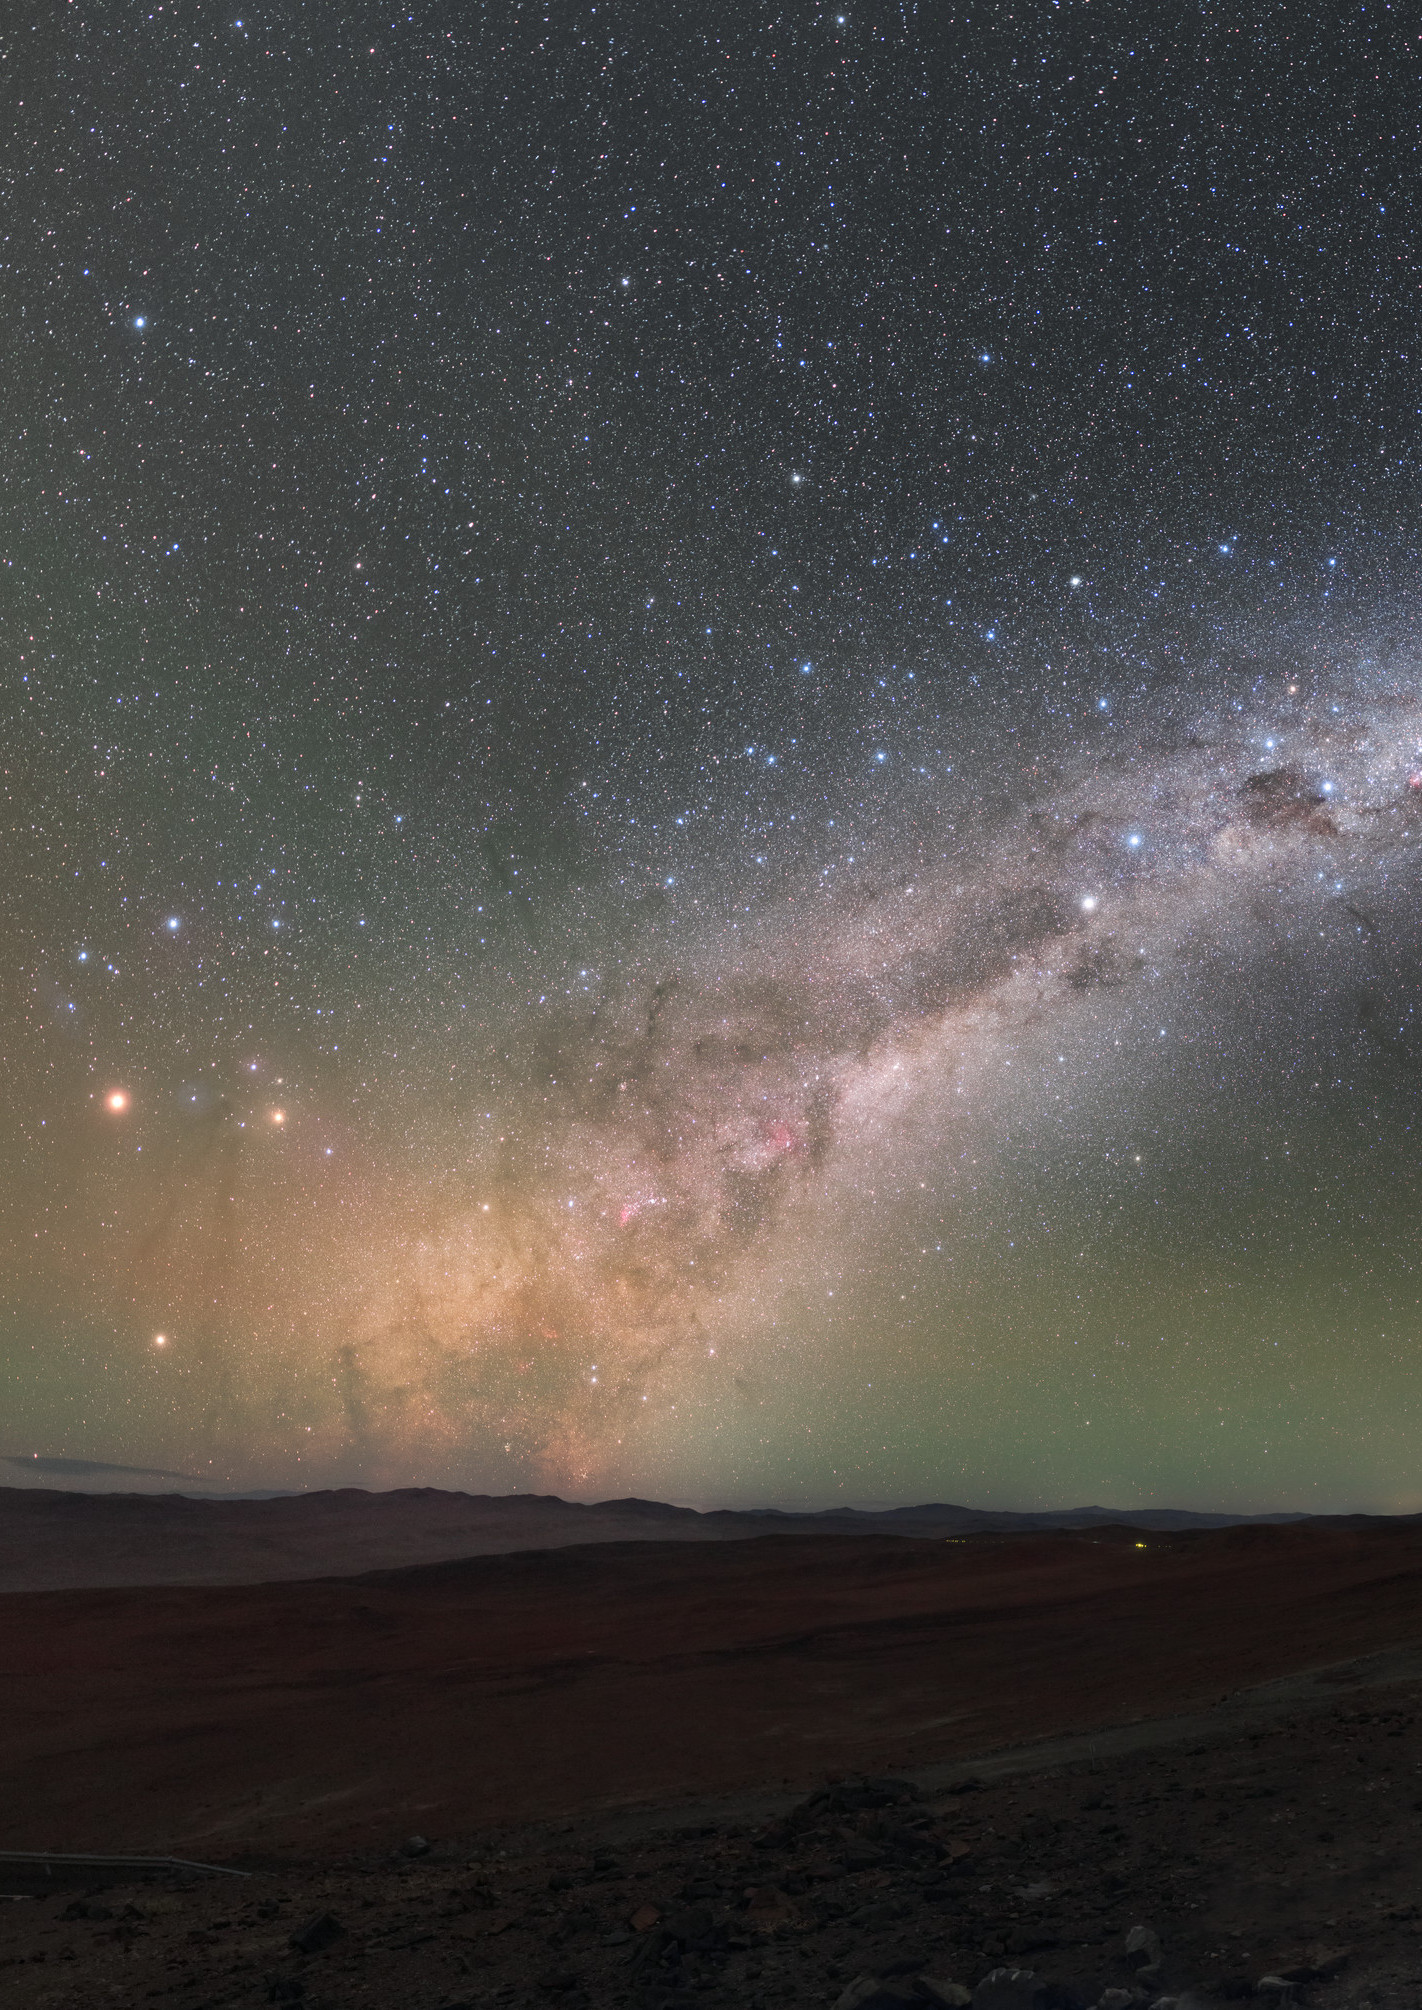
\includegraphics[width=\paperwidth]{Images/VLT1}}
    }
    \BgThispage
    
    \fancyfoot[C]{\color{white}\thepage}
    \fancyfoot[L]{\vspace{3.5ex}\tiny\textcolor{white}{Credit: ESO, P. Hor\'{a}lek}}
    \clearpage
    \newpage

    \renewcommand{\CurrentTitleColor}{\color{white}}
\fi

\chapter{Prospects for observing the low-density cosmic web in \texorpdfstring{\lymana}{\lymanatext} emission}
\label{ch:Prospects_for_observing_the_low-density_cosmic_web_in_Lya_emission}

\ifsetDraft
\else
    \renewcommand{\CurrentTitleColor}{\color{black}}
    
%    \vspace*{\fill}
%    \setlength{\epigraphwidth}{0.9\textwidth}
%    {\color{white} \epigraph{\textit{We can only see a short distance ahead, but we can see plenty there that needs to be done.}}{--- Alan Turing, Computing Machinery and Intelligence (1950)}}
%    \vspace*{\fill}
    
    \backgroundsetup{
        scale=1,
        color=black,
        opacity=1,
        placement=top,
        angle=0,
        contents={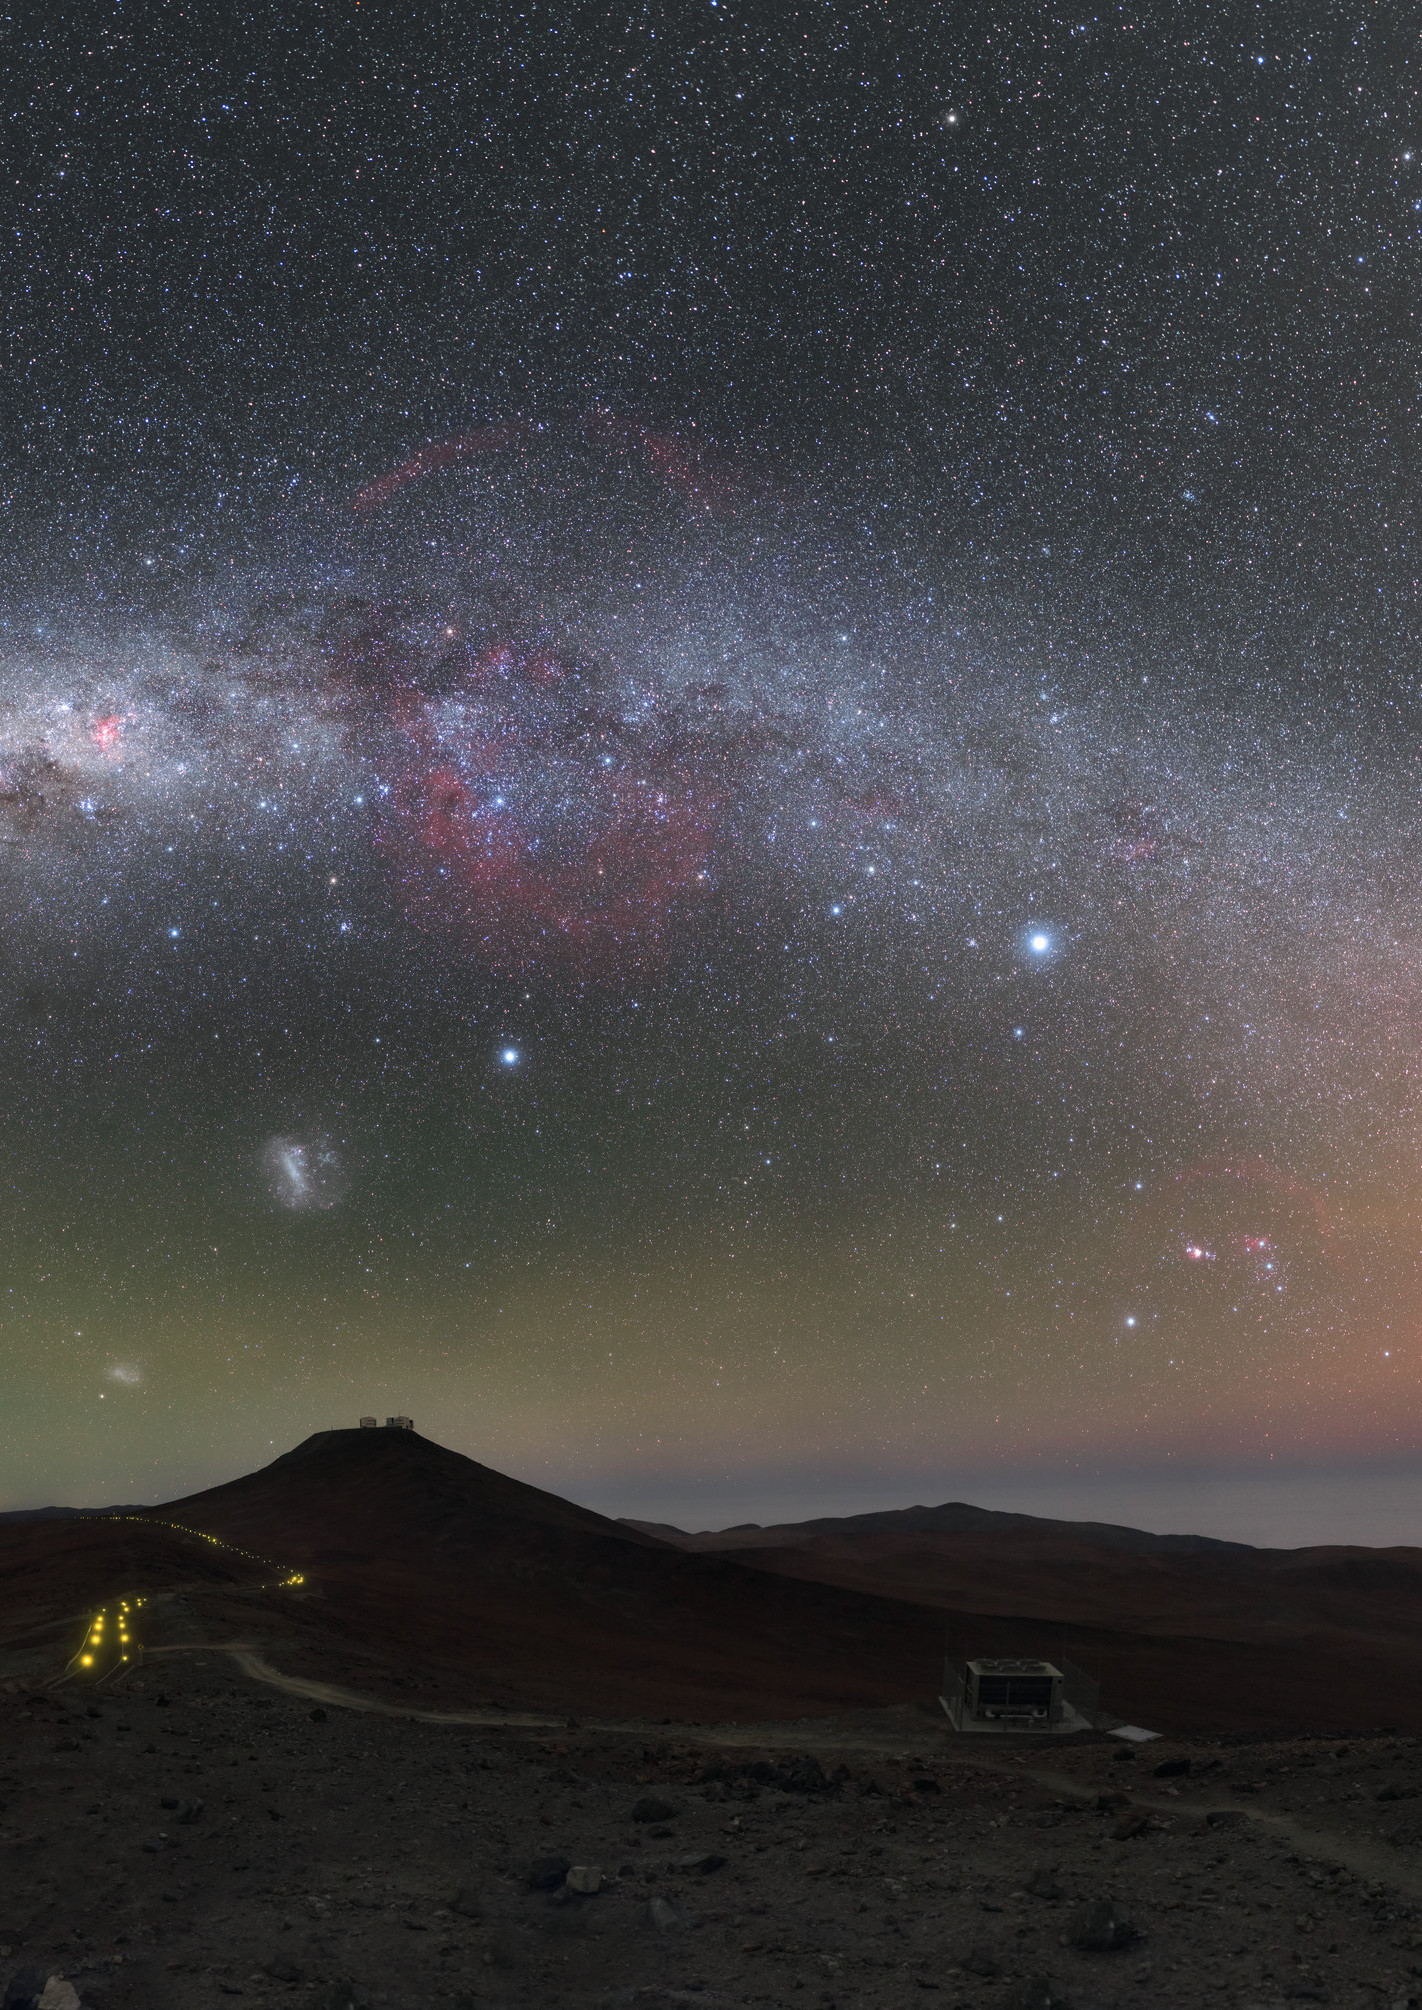
\includegraphics[width=\paperwidth]{Images/VLT2}}
    }
    \BgThispage
    
    \fancyhf{}
    \fancyfoot[C]{\color{white}\thepage}
    \newpage
    \setFancyHdr
\fi

% Reset values used in introduction
%\renewcommand\thefigure{\thechapter.\arabic{figure}}
%\setcounter{figure}{0}

\vspace*{\fill}

\noindent Mapping the IGM in \lya\ emission would yield unprecedented tomographic information on the large-scale distribution of baryons and potentially provide new constraints on the UV background and various feedback processes relevant to galaxy formation. In this chapter, we use a cosmological hydrodynamical simulation to examine the \lya\ emission of the IGM resulting from collisional excitations and recombinations in the presence of a UV background. We focus on gas in large-scale-structure filaments in which \lya\ radiative transfer effects are expected to be moderate. At low density the emission is primarily due to fluorescent re-emission of the ionising UV background as a result of recombinations, while collisional excitations dominate at higher densities. We discuss prospects of current and future observational facilities to detect this emission and find that the emission of filaments of the cosmic web are typically dominated by the halos and galaxies embedded in these filaments, rather than by the lower-density filament gas outside halos. Detecting filament gas directly would require a very long exposure with a MUSE-like instrument on the ELT. Our most robust predictions that act as lower limits indicate this would be slightly less challenging at lower redshifts ($z \lesssim 4$). We also find that there is a large amount of variance between fields in our mock observations. High-redshift protoclusters appear to be the most promising environment to observe the filamentary IGM in \lymana\ emission.

\vspace{3ex}
\begin{mdframed}[backgroundcolor=black!2.5]
    \textsl{This chapter is based on work carried out in collaboration with Ewald Puchwein, Girish Kulkarni, Martin Haehnelt, Renske Smit, and Lewis Weinberger. It appeared in Astronomy \& Astrophysics as \citet*{2021A&A...650A..98W}.}
\end{mdframed}
\vspace*{\fill}

\newpage

\section{Introduction}
\label{chPsec:Introduction}

\lettrine{A}{s the reservoir} of the majority of baryons in the Universe, the IGM presents an invaluable means to understanding the evolution of cosmic structure \citep{2009RvMP...81.1405M}. The IGM has been detected in absorption at a wide range of overdensities out to redshift $z \sim 6$ using \ion{H}{I} \lya\ (see \cref{chIsssec:Photoionisation_by_stars}) absorption lines in the spectra of background quasars (\cref{chIsssec:Cosmic_Reionisation}). Successively larger numbers of quasars have been targeted for this purpose, resulting in a large data set of \lya\ absorption measurements of the IGM. Before reionisation is completed, understanding the physical state of the IGM is complicated by the rather uncertain details of the emergence of the first stars, black holes, and galaxies during the epoch of reionisation, but the post-reionisation ($z \lesssim 5.5$) IGM should be well described by cosmological hydrodynamical simulations \citep{1994ApJ...437L...9C, 1996ApJ...457L..51H, 1999elss.conf..346W, 2017ApJ...837..106O, 2019MNRAS.486.4075O, 2015MNRAS.446.3697L, 2017MNRAS.464..897B}. In these simulations, the observed properties of the IGM are reproduced by a fluctuating gas density distribution tracing the cosmic structure formation process. The gas is thereby in ionisation equilibrium with a uniform UVB created by galaxies and AGN. This has led to constraints on the ionisation and thermal state of the IGM out to $z \sim 6$ \citep{1997ApJ...489....7R, 1999ApJ...511..521D, 2000MNRAS.318..817S, 2003MNRAS.342.1205M, 2008ApJ...688...85F, 2011MNRAS.410.1096B, 2012MNRAS.419.2880B, 2013MNRAS.436.1023B, 2017PhLB..773..258G, 2019ApJ...872...13W, 2019MNRAS.486..769K} derived from \lya\ absorption observations.

In contrast, \lya\ emission from the IGM has received relatively little attention, despite a history of just over half a century of theoretically predicted prospects \citep{1967ApJ...147..868P, 1987MNRAS.225P...1H, 1996ApJ...468..462G, 2001ApJ...562..605F, 2003ApJ...599L...1F, 2005ApJ...622....7F, 2005ApJ...628...61C, 2010ApJ...708.1048K, 2010ApJ...725..633F, 2012MNRAS.423..344R, 2013ApJ...763..132S, 2016MNRAS.462.1961S, 2017ApJ...848...52H, 2019MNRAS.489.2417A, 2020MNRAS.494.5439E}. Observing intergalactic \lya\ emission instead of absorption has distinct advantages. First, unlike absorption \lya\ emission is directly sensitive to the recombination and collisional physics of the neutral as well as the ionised hydrogen content of the IGM and the CGM that feeds the formation and evolution of galaxies. Second, observations of the \lya\ emission allow us to homogeneously probe three-dimensional volumes. Although three-dimensional \lya-forest studies have now become possible owing to the high number density of observed bright quasars \citep[see e.g.][]{2014MNRAS.440.2599C}, the number of such quasars drops rapidly towards high redshifts \citep{2019MNRAS.488.1035K}. Third, observations of \lya\ emission can potentially provide independent constraints on the IGM temperature and photoionisation rate, particularly at densities higher than those probed by the \lya\ forest ($\Delta \gtrsim 10$).

Using narrowband imaging and integral field unit (IFU) imaging, emission in \lya\ from the CGM and/or IGM has now been observed as ``giant \lya\ nebulae'' in the proximity ($\ssim 100\,\mathrm{kpc}$) of radio-loud and radio-quiet quasars \citep{1985ApJ...299L...1D, 1991ApJ...368...28H, 1991ApJ...370...78H, 1990ApJ...365..487M, 2007A&A...461..823V, 2007MNRAS.378..416V, 2008ApJ...672...48C, 2008MNRAS.390.1505H, 2008ApJ...681..856R, 2009A&A...495..471S, 2011MNRAS.418.1115R, 2012MNRAS.425.1992C, 2013MNRAS.429..429R, 2014Natur.506...63C, 2014ApJ...786..106M, 2014MNRAS.443.3795R, 2015Sci...348..779H, 2016ApJ...829....3A, 2016ApJ...831...39B, 2016MNRAS.462.1978F, 2017ASSL..430..195C}. The circumgalactic hydrogen is strongly affected by ionising radiation from these quasars. Observations suggest that the \lya\ emission is mostly recombination radiation and that dense ($n > 1 \, \mathrm{cm^{-3}}$), ionised, and relatively cold ($T \sim 10^4 \, \mathrm{K}$) pockets of gas should surround massive galaxies \citep{2017ASSL..430..195C}.

\lya\ emission can also result from fluorescent re-emission of the ionising UVB radiation. In the last two decades, significant progress has been made in detecting extended \lya\ emission around galaxies \citep{1996ApJ...457..490F, 1999MNRAS.305..849F, 1999AJ....118.2547K, 2000ApJ...532..170S, 2004AJ....128.2073H, 2008ApJ...681..856R, 2011ApJ...736..160S, 2012MNRAS.425..878M, 2013ApJ...762...38P, 2014MNRAS.442..110M, 2016ApJ...832...37G, 2016A&A...587A..98W, 2017ApJ...837...71C, 2017A&A...608A...8L, 2017MNRAS.465.3803V, 2018ApJ...856...72O, 2018Natur.562..229W, 2019MNRAS.482.3162A}. Using deep ($\ssim 30 \, \mathrm{h}$ exposure time) VLT/MUSE observations of the \textit{Hubble} Deep Field South (HDFS) and \textit{Hubble} Ultra-Deep Field (HUDF) reported in \citet{2015A&A...575A..75B, 2017A&A...608A...1B}, the sensitivity of median-stacked radial profiles of \lya\ emission currently reaches a SB of $\ssim 4 \cdot 10^{-21} \, \mathrm{erg \, s^{-1} \, cm^{-2} \, arcsec^{-2}}$ \citep{2018Natur.562..229W}. This faint signal from \lya\ halos can be traced out to projected (physical) galactic radii of $\ssim 60 \, \mathrm{kpc}$ \citep{2018Natur.562..229W}. Even deeper data sets, such as the MUSE Ultra Deep Field \citep[MUDF, described in][]{2019MNRAS.485L..62L} and the MUSE Extremely Deep Field \citep[MXDF, see][]{2021A&A...647A.107B} are beginning to be explored. Both will reach a depth of the order of $\ssim 100 \, \mathrm{h}$ (i.e. reaching a sensitivity of the order of a few times $10^{-20} \, \mathrm{erg \, s^{-1} \, cm^{-2} \, arcsec^{-2}}$). The \lya\ emission coming from the intergalactic gas between galaxies is just beginning to be probed and is the focus of this chapter.

So far, it has proven very difficult to map the spatial distribution of the IGM beyond the CGM and to study its global properties by directly observing the IGM in emission rather than absorption. This has so far only been achieved in special cases, for example in the vicinity of AGN \citep[e.g.][]{2014Natur.506...63C, 2014ApJ...786..106M, 2015Sci...348..779H, 2016ApJ...831...39B, 2019Sci...366...97U}, by applying statistical image processing techniques \citep[][; in this case, the CGM only showed a preferential direction of extension towards neighbouring galaxies, no significant signal of filamentary structure in the IGM was found]{2018MNRAS.475.3854G}, by cross-correlating \lya\ emitters (LAEs) and \lya\ intensity mapping \citep{2021ApJ...916...22K}, by observing the thermal Sunyaev-Zel’dovich effect \citep[e.g.][]{2019A&A...624A..48D, 2019MNRAS.483..223T}, or by detection of warm-hot gas in X-ray emission \citep[e.g.][]{1999A&A...341...23K, 2015Natur.528..105E}.

Building on the work of previous studies \citep[such as those by][]{1996ApJ...468..462G, 2003ApJ...599L...1F, 2005ApJ...628...61C, 2013ApJ...763..132S, 2016MNRAS.462.1961S}, this chapter investigates the possibility of such observations. We explore a simulation run based on the Sherwood simulation project \citep{2017MNRAS.464..897B}, which incorporates an on-the-fly self-shielding model to predict the properties of \lya\ emission from the cosmic web. The simulation is aimed at accurately modelling the IGM and employs a modified version of the uniform meta-galactic UVB model by \citet[; \citetalias{2012ApJ...746..125H} hereafter]{2012ApJ...746..125H} that is calibrated to match observations of the \lya\ forest. The large volume and high dynamic range of the simulation allows us to probe the physical environment of the IGM with well-resolved under- and overdense regions. Moreover, this enables us to study the prospects of an array of current and future observational facilities aiming to detect this emission. We focus on a future reincarnation of VLT/MUSE on next-generation observatories such as the Extremely Large Telescope (ELT) for a more detailed sensitivity analysis.

We describe the simulations used in this chapter in \cref{chPsec:Methodology}, together with our model for \lya\ production in the IGM. \Cref{chPsec:Results} presents our results and a discussion of the detection prospects. We summarise our conclusions in \cref{chPsec:Conclusions}. Throughout this chapter, we adopt the cosmological parameters $\Omega_{\text{m}, \, 0} = 0.308$, $\Omega_{\Lambda, \, 0} = 0.692$, $\Omega_{\text{b}, \, 0} = 0.0482$, and $h=0.678$ (so $H_0 = 67.8 \, \mathrm{km \, s^{-1} \, Mpc^{-1}}$), taken from the best-fitting $\Lambda$CDM model for the combined \textit{Planck}+WP+highL+BAO measurements \citep{2014A&A...571A..16P}. The helium fraction is assumed to be $f_\text{He} = 0.24$.
\begin{figure}
    \centering
    \includegraphics[width=0.6\linewidth]{"Plots/ChapterP/UVB_limits"}
    \caption[Limiting SB and density quantities as a function of redshift]
    {Limiting SB and density quantities as a function of redshift. The top panel shows the limiting SB of \lya\ in the mirror assumption, where $65\%$ of ionising photons in the UVB are reprocessed into \lya\ photons (see text for details) and the bottom panel shows the self-shielding critical density contrast $\Delta_\text{crit}$. The two different lines correspond to UVBs of \citet[, \citetalias{2012ApJ...746..125H}]{2012ApJ...746..125H} and \citet[, \citetalias{2019MNRAS.485...47P}]{2019MNRAS.485...47P}. Above $z>6$, where the line is dashed, the \citetalias{2019MNRAS.485...47P} limits are not representative of ionised bubbles during patchy reionisation because the impact of neutral regions on the effective opacity to hydrogen ionising photons is included in the modelling \citepalias[see][]{2019MNRAS.485...47P} and hence a neutral hydrogen-weighted average over both neutral and ionised regions is computed in that model. A redshift of $z=4.8$ is highlighted by the dashed line.}
    \label{chPfig:UVB_limits}
\end{figure}

\section{Methodology}
\label{chPsec:Methodology}

\lya\ emission from the moderately dense IGM is produced via recombinations and collisional excitations. Recombination is the process in which a free electron is captured by an ion, which in this case is \ion{H}{II}. \lya\ is emitted provided the recombination leaves hydrogen in an excited state and the last step of the resulting series of energy transition(s) is from energy level $n=2$ to $n=1$. Collisional excitation is the effect in which neutral hydrogen (\ion{H}{I}) is excited through a collision with an electron, which can subsequently lead to the emission of \lya\ in the same way as with recombinations. We used a hydrodynamical simulation calibrated to UVB constraints from the \lya\ forest along with an on-the-fly self-shielding prescription to model these processes.

In the analysis, we focus on low-density gas (below the critical density above which self-shielding becomes a dominant process) as we are primarily interested in detecting emission from the cosmic web. At $z=4.8$, this critical density corresponds to an overdensity $\Delta \equiv \rho/\bar{\rho} \simeq 100$ (see \cref{chPsssec:Density limits}). Furthermore, modelling of all relevant feedback and radiative transfer effects becomes increasingly challenging at higher densities.
\begin{figure}
    \centering
    \includegraphics[width=0.6\linewidth]{"Plots/ChapterP/Theoretical_emissivity"}
    \caption[Theoretical \lya\ emissivity as a function of temperature]
    {Normalised emissivity (units are $\mathrm{erg \, s^{-1} \, cm^3}$) of the \lya\ line in a cloud of primordial gas at $z=4.8$ as a result of recombination and collisional excitation processes as a function of temperature. There are three values of density, corresponding to overdensities of $1$, $10$, and $100$, respectively; the mean cosmological hydrogen density corresponds to $\bar{n}_\text{H} = 3.69 \cdot 10^{-5} \, \mathrm{cm^{-3}}$ at this redshift. The dashed and dotted lines show the contribution from just recombination and collisional excitation, respectively.}
    \label{chPfig:Emissivity theoretical}
\end{figure}

\subsection{\texorpdfstring{\lya}{\lyatext} emission through recombination}
\label{chPssec:Lya recombination emission}

\subsubsection{Emissivity}
\label{chPsssec:Recombination emissivity}

The underlying equation governing \lya\ emission resulting from recombination in a gas containing hydrogen is given by \citep[see e.g.][]{2014PASA...31...40D, 2016MNRAS.462.1961S}
\begin{equation}
    \label{chPeq:Recombination emissivity}
    \epsilon_\text{rec}(T) = f_\text{rec, A/B} (T) \, n_\text{e} \, n_\text{\ion{H}{II}} \, \alpha_\text{A/B}(T) \, E_\text{\lya} \, ,
\end{equation}

\noindent where $\epsilon_\text{rec}$ is the \lya\ luminosity density (in units of $\mathrm{erg \, s^{-1} \, cm^{-3}}$) as a function of the temperature $T$ of the gas. In this equation, $f_\text{rec, A/B}$ is the fraction of case-A or case-B recombinations, which ultimately result in the emission of a \lya\ photon; and the free electron and \ion{H}{II} number densities are denoted by $n_\text{e}$ and $n_\text{\ion{H}{II}}$, respectively. Case A and case B refer to the way in which recombination occurs. All possible recombinations of \ion{H}{II} and a free electron are considered in case A; this includes any recombination event that take the resulting neutral hydrogen directly to the ground state ($n=1$). In case B, only recombinations resulting in hydrogen in an excited state are considered. The recombination coefficient given in unit volume per unit time ($\mathrm{cm^{3} \, s^{-1}}$) for case-A or -B recombination is denoted by $\alpha_\text{A/B}$, and $E_\text{\lya}$ is the energy of a \lya\ photon.

Since direct recombinations into the ground state do not result in \lya\ emission, an appropriately lower fraction that results in \lya\ emission, $f_\text{rec, A} < f_\text{rec, B}$, has to be used if $\alpha_\text{A}$ rather than $\alpha_\text{B}$ is adopted as the recombination coefficient. The luminosity densities obtained for case A and case B are then equivalent, except for minor differences due to different fitting functions for the coefficients. We chose to fix our calculations to use case-B coefficients. We modelled $f_\text{rec, B}$ using the relations given by \citet{2008ApJ...672...48C} and \citet{2014PASA...31...40D}, whose fitting formulae are presented in \cref{appPsec:Model parameters}; for example at $T = 10\,000 \, \mathrm{K}$, this fraction is $\ssim 0.68$. We elected to use case B because the model for $f_\text{rec, A} (T)$ from \citet{2014PASA...31...40D} is only valid up to $\ssim 10^{6.5} \, \mathrm{K}$, whereas gas temperatures in our simulations range up to $\ssim 10^{7} \, \mathrm{K}$ (\cref{chPssec:Surface brightness maps}). For the recombination coefficient, $\alpha_\text{B}(T)$, we adopted the fitting function given in \citet{2011piim.book.....D}. The precise expressions can also be found in \cref{appPsec:Model parameters}.

\subsubsection{Mirror limit}
\label{chPsssec:Mirror limit}

In the absence of local ionising UV sources and significant collisional ionisation, the recombination contribution to \lya\ emission should not exceed the SB expected from fully absorbing the external UVB at the boundaries of self-shielded regions and fluorescently re-emitting a corresponding number of \lya\ photons, hence ``mirroring'' the external UVB. In calculating the recombination contribution to \lya\ emission, unless mentioned otherwise, we employed this mirror assumption as an upper limit. More precisely, we placed an upper $\text{SB}$ limit at the value expected when $65\%$ of the ionising UVB is reprocessed as \lya\ photons \citep[e.g.][]{1996ApJ...468..462G, 2005ApJ...628...61C}, equal to $\text{SB} \simeq 3.29 \cdot 10^{-21} \, \mathrm{erg \, s^{-1} \, cm^{-2} \, arcsec^{-2}}$ for a \citetalias{2012ApJ...746..125H} UVB at $z=4.8$. \Cref{chPfig:UVB_limits} shows the mirror limit for two different UVBs from \citetalias{2012ApJ...746..125H} and \citet[; \citetalias{2019MNRAS.485...47P} hereafter]{2019MNRAS.485...47P}.

In reality, local ionising sources can boost the recombination emission above the mirror limit. Predicting this reliably is, however, extremely challenging because it involves modelling the ionising source populations in galaxies and the escape of ionising radiation from galaxies in full detail. Our recombination contribution to \lya\ emission computed assuming the mirror limit should hence be considered only as a robust lower limit.

\subsection{\texorpdfstring{\lya}{\lyatext} emission through collisional excitation}
\label{chPssec:Lya collisional excitation emission}

\subsubsection{Emissivity}
\label{chPsssec:Collisional excitation emissivity}

For collisional excitation, the \lya\ luminosity density has a similar form \citep{1990MNRAS.242..692S, 1991ApJ...380..302S, 2014PASA...31...40D, 2016MNRAS.462.1961S} given by
\begin{equation}
    \label{chPeq:Collisional excitation emissivity}
    \epsilon_\text{exc}(T) = \gamma_\text{1s2p} (T) \, n_\text{e} \, n_\text{\ion{H}{I}} \, E_\text{\lya} \, ,
\end{equation}

\noindent where $n_\text{\ion{H}{I}}$ denotes the number density of neutral hydrogen. We used the fitting functions for the collisional excitation coefficient $\gamma_\text{1s2p}$ given by \citet{1990MNRAS.242..692S} and \citet{1991ApJ...380..302S}. These fitting functions are valid in the temperature range $2 \cdot 10^3 \, \mathrm{K} \leq T \leq 1 \cdot 10^8 \, \mathrm{K}$ (cf. \cref{appPsec:Model parameters}). The rates are not identical to those applied in the cosmological hydrodynamical simulation (see \cref{chPssec:SherwoodSuite}) as these are only given as an ensemble rather than for the specific $2p \rightarrow 1s$ transition in which \lya\ is emitted, but in the relevant temperature regime deviate so little that gas cooling equilibrium would not be appreciably violated.

\subsubsection{Density limits}
\label{chPsssec:Density limits}

When computing the \lya\ luminosity due to collisional excitation, we only considered gas well below the critical self-shielding density that is derived for the appropriate UVB (the \citetalias{2012ApJ...746..125H} UVB, unless mentioned otherwise). We made use of the critical self-shielding hydrogen number density at $T = 10^4 \, \mathrm{K}$ given in equation (13) in \citet{2013MNRAS.430.2427R} for this purpose (shown in the bottom panel of \cref{chPfig:UVB_limits} as a density contrast), but since this is based on the column density distribution of neutral hydrogen and for the purpose of absorption instead of emission processes, we chose a conservative default density threshold at half this value.

As shown in \cref{chPfig:UVB_limits}, the critical self-shielding overdensity is $\Delta_\text{crit} \simeq 100$ at $z=4.8$. We note that the density contrast, $\Delta_\text{crit}$, decreases towards higher redshift, meaning gas starts to be affected by self-shielding at a lower overdensity at higher redshift. By focussing on gas with densities below this critical threshold, we additionally ensure at this redshift that we do not enter the realm of gas densities strongly affected by the detailed baryonic physics of galaxy formation, such as feedback processes. For this reason, most of the results presented in this chapter are chosen to be at $z=4.8$ and are again a robust lower limit.

\subsection{Emissivity}
\label{chPssec:Emissivity}

\Cref{chPfig:Emissivity theoretical} shows the \lya\ luminosity density at $z=4.8$ as a function of gas temperature for a gas of primordial composition at three different overdensities of $1$, $10$, and $100$; the mean cosmological hydrogen density corresponds to $\bar{n}_\text{H} = 3.69 \cdot 10^{-5} \, \mathrm{cm^{-3}}$ at this redshift. To derive the corresponding neutral hydrogen densities, we assume that hydrogen is in ionisation equilibrium with the \citetalias{2012ApJ...746..125H} UVB at $z=4.8$. \Cref{chPfig:Emissivity theoretical} also shows the recombination and collisional excitation components of the total \lya\ emission. We find that collisional excitation dominates at high temperatures ($T \gtrsim 2 \times 10^4 \, \mathrm{K}$).

\subsection{Cosmological hydrodynamical simulation}
\label{chPssec:SherwoodSuite}

To estimate the cosmological \lya\ signal with the theoretical framework above, we made use of a simulation that builds upon the Sherwood simulation project \citep{2017MNRAS.464..897B}. The simulation is performed with the energy- and entropy-conserving TreePM smoothed particle hydrodynamics (SPH) code \program{p-gadget-3}, which is an updated version of the publicly available \program{gadget-2} code \citep{2001NewA....6...79S, 2005MNRAS.364.1105S}. In this chapter, we used the same volume as in the 40--1024 simulation of the Sherwood suite. A periodic, cubic volume $40 \, h^{-1} \, \mathrm{cMpc}$ long was simulated, employing a softening length of $l_\mathrm{soft}=1.56 \, h^{-1} \, \mathrm{ckpc}$, and $1024^3$ dark matter and gas particles. Initial conditions were set up at redshift $z=99$ and the simulation was evolved down to $z=2$. In order to speed up the simulation, star formation was simplified using the implementation of \citet{2004MNRAS.354..684V} in \program{p-gadget-3}; this method converts gas particles, with temperatures less than $10^5 \, \mathrm{K}$ and densities of more than a thousand times the mean baryon density, to collisionless stars. This approximation is appropriate for this chapter as we do not consider the \lya\ emission from the interstellar medium of galaxies, where a complex set of \lya\ radiative transfer processes need to be accounted for. The ionisation and thermal state of the gas in the simulation is derived by solving for the ionisation fractions under the assumption of an equilibrium with the meta-galactic UVB modelled according to \citetalias{2012ApJ...746..125H}. A small modification to this UVB is applied at $z<3.4$ \citep[see][]{2017MNRAS.464..897B} to result in IGM temperatures that agree with measurements by \citet{2011MNRAS.410.1096B}. We also accounted for self-shielding of dense gas with an on-the-fly self-shielding prescription based on \citet{2013MNRAS.430.2427R}. For each SPH particle and each time step, our modified \program{p-gadget-3} version computes a suppression factor for the UVB due to self-shielding that is based on the local gas density and uses the parameters given in the first line of table~A1 of \citet{2013MNRAS.430.2427R}. This factor is applied to photoionisation and heating rates before they are used in the chemistry and cooling solver. The solver follows photoionisation, collisional ionisation, recombination, and photoheating for gas of a primordial composition of hydrogen and helium, as well as further radiative cooling processes such as collisional excitation, Bremsstrahlung (see \citealt{1996ApJS..105...19K} for the relevant equations), and inverse Compton cooling off the cosmic microwave background \citep{1986ApJ...301..522I}. Metal enrichment and its effect on cooling rates are ignored. We identify dark matter halos in the output snapshots using a friends-of-friends algorithm.

\subsubsection{Narrowband images}
\label{chPsssec:Narrowband}
\begin{figure}[t]
    \centering
    \includegraphics[width=0.6\linewidth]{"Plots/ChapterP/Global_luminosity"}
    \caption[Redshift evolution of the \lya\ luminosity density]
    {Redshift evolution of the comoving \lya\ luminosity density. The blue and orange lines show the results for recombination and collisional excitation emission for gas at densities below half the critical self-shielding density roughly corresponding to the IGM at an overdensity $\Delta \equiv \rho/\bar{\rho} \lesssim 50$ at $z=4.8$ (see \cref{chPsssec:Density limits}). The black line shows the total luminosity density for gas below this density threshold; all these follow from the simulation run with a box size of $40 \, h^{-1} \, \mathrm{cMpc}$ and resolution of $2 \times 1024^3$ particles (see \cref{chPssec:SherwoodSuite} for more details on the simulation). Observational measurements at low redshift ($z<3$), as presented in \citet{2019ApJ...877..150C}, have been included as a reference. These consist of luminosity densities of just galaxies and the contribution of galaxies and AGN (shown as the grey and blue shaded areas, respectively) inferred by \citet{2019ApJ...877..150C} from the intrinsic luminosity density presented in \citet{2017ApJ...848..108W}; the measurement and upper limit from \citet{2019ApJ...877..150C} are shown in red, and the upper limit from \citet{2018MNRAS.481.1320C} \citep[converted to a luminosity density by][]{2019ApJ...877..150C} is shown in black (see text for details). Data points are shown as circles, upper limits as downward triangles. Also shown is the $(1+z)^3$ scaling relation for recombination emission discussed in the text.}
    \label{chPfig:z_evolution_lum}
\end{figure}

When calculating the SB, we constructed mock narrowband images of the simulations, which are images that replicate the result of the process of capturing a narrowband image with a telescope, by taking a thin slice of the simulation in a direction parallel to a face of the simulation box and converting the emissivity in the simulation to arrive at a SB map; this is discussed in more detail below. The slice thickness corresponds to an observed wavelength width $\Delta\lambda_\text{obs}$ of the narrowband. Its redshift range is given by
\begin{equation}
    \Delta z = \frac{\Delta \lambda_\text{obs}}{\lambda_\text{\lya}} \, ,
\end{equation}

\noindent which corresponds to a comoving distance (cf. \cref{chIssec:Observers_in_an_expanding_universe,chIsssec:Cosmological_observables})
\begin{equation}
    \Delta l = \frac{c}{H_0} \int_{z}^{z+\Delta z} \frac{1}{\sqrt{\Omega_{\text{m}, \, 0} \left( 1 + z' \right)^3 + \Omega_{\Lambda, \, 0}}} \dif z' \, .
\end{equation}

As a reference value for the observed narrowband width, we used $\Delta \lambda_\text{obs} = 8.75 \, \text{Å}$, the median value of narrowband widths in the study by \citet{2016A&A...587A..98W}; this corresponds to $7$ spectral pixels of the VLT/MUSE instrument (\cref{chPssec:Observing facilities} describes narrowband imaging in more detail). At a redshift of $z=4.8$, this results in a comoving line-of-sight distance of $\ssim 2.7 \, h^{-1} \, \mathrm{cMpc}$ (see \cref{chPsssec:Density limits} for an elaboration on the choice of this particular redshift), corresponding to only a small fraction of the total size of the simulation volume. We discuss the effect of varying the narrowband width on the detectability of \lya\ further in \cref{chPsssec:Cosmic variance and narrowband widths}.

Using the temperature, density, and ionisation fraction, an emissivity for each individual simulation particle within the narrowband slice can be computed. These emissivities were then converted to luminosities and projected onto a two-dimensional plane using the SPH kernel of the simulation particles, turning them into a luminosity per unit area, which in turn is converted to a SB (see \cref{chIsssec:Cosmological_observables}).

\subsubsection{Radiative transfer effects}
\label{chPsssec:Radiative transfer effects}

In the predictions made in this chapter, \lya\ propagation is always treated in the optically thin limit. For the constructed mock narrowband images, it is assumed that \lya\ photons are emitted in an isotropic manner and reach the observer without any scattering. The exact effects that scattering would have are difficult to accurately predict given for example that the effects of dust are poorly constrained. But it is expected that for the filamentary IGM, the difference between our simulations and a model with a physically accurate treatment of radiative transfer is mostly influenced by two competing effects. First, there might be a broadening of the filamentary structure due to scattering in the nearby IGM, causing the signal to become fainter. Second, however, filaments may also be illuminated by \lya\ radiation coming from nearby dense structures (where additional radiation is likely to be produced in galaxies) that is scattered in the filament, which would cause the filaments to appear brighter. Simulations including radiative transfer show a mixture of these two effects, where the SB of filaments generally is not affected much or is even boosted \citetext{private communication, Weinberger, 2019}. As the effects of radiative transfer on this chapter are expected to be moderate, they are assumed not to affect our main findings in a major way; a more detailed discussion on the optical depth of \lya\ is included in \cref{appPsec:Lya optical depth}. Future work can detail the precise effects of radiative transfer.

We limit the maximum SB from recombinations to what is expected from purely reprocessing or mirroring the UVB at the boundaries of self-shielded regions (see \cref{chPsssec:Mirror limit}). This also mitigates the effect where the absence of radiative transfer can bias the SB upwards in cases in which a sightline crosses several dense structures. In reality, however, with the presence of local ionising sources in such dense regions, an amplification with respect to the reprocessed UVB would likely be present as well. This is also suggested by a comparison of our simulation with a post-processing radiative transfer simulation of the same volume using a local source population similar to that described in \citet{2019MNRAS.485L..24K}. Still, even with an accurate treatment of radiative transfer, the precise effects in the densest regions may rely considerably on the exact baryonic feedback mechanisms that are operating in these regions.
\begin{figure}
    \centering
    \includegraphics[width=\linewidth]{"Plots/ChapterP/Overview_SB_map"}
    \caption[Total \lya\ surface brightness at $z=4.8$]
    {\lya\ SB resulting from the combination of recombination emission (of all gas in the simulation) below the mirror limit and collisional excitation of gas below half the critical self-shielding density, covering an area of $20 \times 20 \, \mathrm{arcmin}^2$, or $31.0 \times 31.0 \, h^{-2} \, \mathrm{cMpc}^2$, in a narrowband with $\Delta \lambda_\text{obs} = 8.75 \, \Angstrom$ (corresponding to $\ssim 2.7 \, h^{-1} \, \mathrm{cMpc}$) in a simulation snapshot at $z=4.8$. The images are made by the projection method (\cref{chPsssec:Narrowband}) onto a pixel grid of $6000 \times 6000$; this is the same pixel size as MUSE, making this image the equivalent of a mosaic of $20 \times 20$ MUSE pointings (more details on MUSE follow in \cref{chPssec:Observing facilities}). Regions 1 and 2, indicated by the white rectangles, will be studied in more detail later. Also shown in the bottom left corner are the scales of the MUSE field of view ($1 \times 1 \, \mathrm{arcmin}^2$) and $1 \, h^{-1} \, \mathrm{cMpc}$.}
    \label{chPfig:SB}
\end{figure}
\begin{figure}
    \centering
    \includegraphics[width=\linewidth]{"Plots/ChapterP/Recombination_collisional_excitation_maps"}
    \caption[\lya\ surface brightness of recombination and collisional excitation processes at $z=4.8$]
    {\lya\ SB of recombination (panel~\textbf{a}) and collisional excitation (panel~\textbf{b}) processes in a simulation snapshot at $z=4.8$, for the gas at densities below half the critical self-shielding density in a narrowband with $\Delta \lambda_\text{obs} = 8.75 \, \Angstrom$, or $\ssim 2.7 \, h^{-1} \, \mathrm{cMpc}$; the projections are made with pixel grid sizes of $1024 \times 1024$. These images show the entire (two-dimensional) spatial extent of the simulation, $40 \times 40 \, h^{-2} \, \mathrm{cMpc}^2$ ($25.8 \times 25.8 \, \mathrm{arcmin}^2$). Panels~\textbf{c} and \textbf{d} show the same maps, but without a density cut-off.}
    \label{chPfig:SBrecexc}
\end{figure}

\section{Results}
\label{chPsec:Results}

\subsection{Luminosity density}
\label{chPssec:Luminosity density}

\Cref{chPfig:z_evolution_lum} shows the redshift evolution of the comoving \lya\ luminosity density in our simulation down to $z=2$. The total luminosity of gas within the entire simulation at densities below half the critical self-shielding density, corresponding to an overdensity $\rho/\bar{\rho} \lesssim 50$ at $z=4.8$ (see \cref{chPsssec:Density limits}), roughly corresponding to the IGM, is computed. This is also done separately for the recombination and collisional excitation contributions. We then divide by the (comoving) simulation volume to convert the luminosity to a comoving luminosity density.

Observational measurements at low redshift ($z<3$), as compiled by \citet{2019ApJ...877..150C}, are included as reference. We note that these data points should not be directly compared to our predictions as we consider only emission from the low-density gas in the IGM. The data consist of estimates of the luminosity density of \lya\ emission from galaxies and AGN inferred by \citet{2017ApJ...848..108W} based on a flux-limited sample of LAEs from GALEX (Galaxy Evolution Explorer) data and scaling the H$\alpha$ galaxy luminosity function measurements \citep{2013MNRAS.428.1128S} out to $z=2$. \citet{2019ApJ...877..150C} obtain a measurement on the total \lya\ luminosity density from galaxies and AGN as well as an upper limit on the diffuse IGM contribution by cross-correlating the GALEX UV intensity maps with spectroscopic objects in the Sloan Digital Sky Survey (SDSS). A comparison of the measurements from \citet{2019ApJ...877..150C} and \citet{2017ApJ...848..108W} indicates that, at least at $z \lesssim 1$, most \lya\ emission originates in galaxies and AGN. The upper limit from \citet[; converted to a luminosity density by \citealt{2019ApJ...877..150C}]{2018MNRAS.481.1320C} is shown in black in \cref{chPfig:z_evolution_lum}. \citet{2018MNRAS.481.1320C} fit model spectra to luminous red galaxies in the Baryon Oscillation Spectroscopic Survey (BOSS) and cross-correlate the residual \lya\ emission with the \lya\ forest in BOSS quasars to obtain the upper limit from a non-detection shown in \cref{chPfig:z_evolution_lum}. As such, this procedure places a limit on the component of diffuse \lya\ emission that correlates with the matter distribution \citep{2018MNRAS.481.1320C}.\footnote{An additional measurement, arising from a cross-correlation with BOSS quasars, is restricted to scales within $15 \, h^{-1} \, \mathrm{cMpc}$ of a quasar \citep[equivalent to only $\ssim 3\%$ of space, see][]{2018MNRAS.481.1320C} and is therefore not included as a global luminosity density in this chapter.}

Going from redshift $z=2$ to $z=7$, the comoving \lya\ luminosity density increases by just under an order of magnitude (see \cref{appPsec:Redshift evolution} for a further discussion of the redshift evolution of SB). As can be seen in the figure, this is mostly due to the increase in recombination emission. Under the simple assumption that the emissivity is produced at a fixed overdensity its emissivity increases like the square of the mean density, which would correspond to a scaling of
\begin{align}
    \label{chPeq:Recombination emissivity scaling}
    \epsilon_\text{rec} & \sim \Delta^2 (1+z)^6 \text{ (physical luminosity density) or} \\ \nonumber
    \epsilon_\text{rec} & \sim \Delta^2 (1+z)^3 \text{ (comoving luminosity density),}
\end{align}
where $\epsilon_\text{rec}$ is the recombination emissivity and $\Delta \equiv \rho/\bar{\rho}$ the overdensity. As shown by the dashed line in \cref{chPfig:z_evolution_lum}, the simple scaling for recombination emission in \cref{chPeq:Recombination emissivity scaling} explains the simulated luminosity density very well at all redshifts shown.

For collisional excitation, there should be two relevant effects: in the optically thin limit, the neutral fraction in ionisation equilibrium increases proportional to the density, hence $n_\text{\ion{H}{I}} \sim n_\text{H}^2$; consequently, the emissivity scales as $\epsilon_\text{exc} \sim n_\text{\ion{H}{I}} n_\text{e} \sim n_\text{H}^3$. If the emission were again produced at fixed overdensity, and if there is little evolution in the photoionisation rate, this would hence scale as
\begin{align}
    \label{chPeq:Collisional emissivity scaling}
    \epsilon_\text{rec} & \sim \Delta^3 (1+z)^9 \text{ (physical luminosity density) or} \\ \nonumber
    \epsilon_\text{rec} & \sim \Delta^3 (1+z)^6 \text{ (comoving luminosity density),}
\end{align}
where $\epsilon_\text{exc}$ is the emissivity from collisional excitation. However, collisional excitation does not follow the predicted $(1+z)^6$ scaling in \cref{chPeq:Collisional emissivity scaling} (and hence is not shown), even decreasing with redshift at $z \gtrsim 3$. This suggests that it is dominated by emission near the critical self-shielding density (see also \cref{chPssec:Surface brightness maps}) and is hence more strongly affected by the density limit at half the critical self-shielding density, which decreases with increasing redshift more strongly than the mean density (i.e. the critical self-shielding overdensity decreases towards higher redshift, see \cref{chPsssec:Density limits}). Still, we note that, depending on the precise distribution of self-shielded regions, which is dictated by local ionising sources on a small scale, collisional excitation from dense gas could account for an additional increase of the comoving luminosity density that surpasses the cosmic SB dimming effect, which itself scales as $(1+z)^4$.

\subsection{Surface brightness maps}
\label{chPssec:Surface brightness maps}

\cref{chPfig:SB} shows a SB map that is the combination of recombination emission (of all gas in the simulation) below the mirror limit and collisional excitation of gas below half the critical self-shielding density in a simulation snapshot at $z=4.8$, for a narrowband with $\Delta \lambda_\text{obs} = 8.75 \, \Angstrom$ (at this redshift coinciding with a thickness of the slice of $\ssim 2.7 \, h^{-1} \, \mathrm{cMpc}$). The map shows a region corresponding to $20 \times 20 \, \mathrm{arcmin}^2$. Also shown in the bottom left corner is the size of the MUSE field of view (FoV; $1 \times 1 \, \mathrm{arcmin}^2$ -- see \cref{chPssec:Observing facilities} for more details). Regions 1 and 2, indicated by the white rectangles, will be studied in more detail later. The values of the SB for this narrowband width are of the order of $\text{SB} \lesssim 10^{-23} \, \mathrm{erg \, s^{-1} \, cm^{-2} \, arcsec^{-2}}$ for the void regions, increasing to typically $\ssim 10^{-21} \, \mathrm{erg \, s^{-1} \, cm^{-2} \, arcsec^{-2}}$ for the IGM filaments. The denser regions have intensity peaks that typically show SB values of $\ssim 10^{-20} \, \mathrm{erg \, s^{-1} \, cm^{-2} \, arcsec^{-2}}$.

\cref{chPfig:SBrecexc} shows the same narrowband slice as in \cref{chPfig:SB} (now for the full spatial extent of the simulation box, $40 \times 40 \, h^{-2} \, \mathrm{cMpc}^2$ or $25.8 \times 25.8 \, \mathrm{arcmin}^2$) split into contributions from recombination and collisional excitation processes in the gas. These maps were all made by projection onto a grid of $1024 \times 1024$ pixels. As before, a narrowband slice with $\Delta \lambda_\text{obs} = 8.75 \, \Angstrom$ ($\ssim 2.7 \, h^{-1} \, \mathrm{cMpc}$) was chosen. Panels~a and b show gas at densities below half the critical self-shielding density, while panels~c and d show all gas. The mirror limit was applied to both panels showing recombination emission (a and c). In this large-scale narrowband image, the total luminosity of recombination processes below half the critical self-shielding density -- that is the total in panel~a before imposing the mirror limit (although no pixels are in fact above the limit in this panel) -- is $\ssim 1.75 \cdot 10^{43} \, \mathrm{erg \, s^{-1}}$. For collisional excitation (the total in panel~b), this is $\ssim 5.45 \cdot 10^{42} \, \mathrm{erg \, s^{-1}}$. Including all gas, the total luminosity is $\ssim 5.02 \cdot 10^{43} \, \mathrm{erg \, s^{-1}}$ for recombination (panel~c), again before imposing the mirror limit (now only $0.37\%$ of pixels are above the limit); the total value is $\ssim 2.21 \cdot 10^{44} \, \mathrm{erg \, s^{-1}}$ for collisional excitations (panel~d). We note that while collisional excitations dominate over recombinations at high densities, the two processes contribute more equally at the lower densities prevalent in large-scale-structure filaments; recombination prevails slightly over collisional excitation below our adopted threshold. Moreover, gas near or somewhat above the critical self-shielding density contributes significantly to the maximum SB that is reached for both channels. We conclude that the recombination prediction including all gas while the mirror limit is imposed should yield at least a robust lower limit, while the collisional excitation prediction for gas at higher densities is more uncertain, thereby motivating our conservative density limit (\cref{chPsssec:Density limits}).
\begin{figure}[t]
    \centering
    \includegraphics[width=\linewidth]{"Plots/ChapterP/Phase_space_luminosity"}
    \caption[\lya\ luminosities of recombination and collisional excitation processes in phase space at $z=4.8$]
    {Histogram of \lya\ luminosities of recombination (panel~\textbf{a}) and collisional excitation (panel~\textbf{b}) processes in the same region as shown in \cref{chPfig:SBrecexc} (a narrowband with $\Delta \lambda_\text{obs} = 8.75 \, \Angstrom$, equivalent to $\ssim 2.7 \, h^{-1} \, \mathrm{cMpc}$) in a simulation snapshot at $z=4.8$ in phase space. The colour represents the total luminosity in the simulation per histogram bin. The horizontal dashed line corresponds to the lower limit above which the fitting function of \citet{1990MNRAS.242..692S} and \citet{1991ApJ...380..302S} for collisionally excited \lya\ emission is valid; the upper limit lies above the plotted range. The vertical dotted line shows the critical self-shielding density threshold at this redshift for the \citetalias{2012ApJ...746..125H} UVB \citep[from equation (13) in][]{2013MNRAS.430.2427R}. Densities above the threshold are also more strongly affected by modelling uncertainties.}
    \label{chPfig:Luminosity phase space}
\end{figure}

While overall these SB maps exhibit the same structure as \cref{chPfig:SB}, the spatial distribution of emission coming from collisional and recombination processes is different. The degree of clustering in the emission is lower for the emission produced by recombination processes than it is for the contribution of collisional excitation. Recombination and collisional excitation depend differently on temperature and density, as discussed in \cref{chPssec:Luminosity density}. In particular, at fixed temperature and photoionisation rate, recombinations are proportional to the square of the density, $\ssim \rho^2$, while in ionisation equilibrium collisional excitations are proportional to $\ssim \rho^3$. As a consequence, recombinations are more equally spread across the volume, while collisional excitations are clearly more important at higher densities, thus reflecting the filamentary structure of the cosmic web better and leaving darker voids in between. To understand this in more detail, we now turn to the phase-space distribution of the gas in the simulation.

In \cref{chPfig:Luminosity phase space}, the luminosity in the simulation is shown at the same redshift and the same region as in \cref{chPfig:SBrecexc} (also in the identical narrowband slice of $\Delta \lambda_\text{obs} = 8.75 \, \Angstrom$, or $\ssim 2.7 \, h^{-1} \, \mathrm{cMpc}$), now as a luminosity-weighted, two-dimensional histogram in temperature and density. This illustrates what was discussed in \cref{chPssec:Luminosity density} and shown in \cref{chPfig:SBrecexc}: collisional excitation is not effective at lower densities and the most luminous gas particles are located in the upper part of the very high-density cooling branch. Recombination emission, on the other hand, exhibits luminosities that are more comparable at lower and higher densities.

From the phase-space distribution in \cref{chPfig:Luminosity phase space}, it is clear that very little gas has temperatures outside of the temperature range of $2 \cdot 10^3 \, \mathrm{K} \leq T \leq 1 \cdot 10^8 \, \mathrm{K}$, for which our fitting function for collisionally excited \lya\ is valid. The lower limit of this fitting function is indicated by the horizontal dashed line; the upper limit lies above the plotted range and almost all of the gas in the simulation.\footnote{This is the case for the entire relevant redshift range.} The contribution from gas outside of this temperature range will be very small and we thus neglect it here.

The vertical dotted line shows the critical self-shielding density threshold at this redshift for the \citetalias{2012ApJ...746..125H} UVB \citep[from equation (13) in][]{2013MNRAS.430.2427R}, illustrating the limiting density below which gas is not be strongly affected by the details of modelling self-shielding. 

\begin{landscape}
    \begin{table}
        \centering
        \caption[Observational experiments]{
            Overview of a selection of current and future instruments that might be most promising for detecting IGM filaments. Fields left blank indicate currently unknown or undecided values. All current instruments presented are IFU spectrographs, upcoming and/or proposed instruments include several IFU spectrographs and space telescopes (two UV satellites and one IR spectrophotometer). Future experiments are in the development stage, unless marked with an asterisk.
        }
        \begin{tabular}{lcccccc}
            \hline
            Name & Wavelength range & Redshift range & Field of view  & Resolution \\
            & $\lambda$ (\Angstrom)& $z_\mathrm{\lya}$ &  & $R$ \\
            \hline 
            \textit{Current IFU instrumentation} & & & & \\
            \hline 
            KCWI-Blue (Keck) & $3500$-$5600$ & $1.9$-$3.6$ & $20 \times 33 \, \mathrm{arcsec}^2$  & $1000$-$20000$ \\
            MUSE (VLT) & $4650$-$9300$ & $2.8$-$6.7$ & $1 \times 1 \, \mathrm{arcmin}^2$  & $1770$-$3590$ \\
            KMOS (VLT) & $8000$-$25000$ & $5.6$-$19.6$ & $ 65 \times 43 \, \mathrm{arcsec}$  & $2000$-$4200$ \\
            OSIRIS (Keck) & $10000$-$24500$ & $7.2$-$19.1$ & $4.8 \times 6.4  \, \mathrm{arcsec}^2$ & $2000$-$4000$ \\
            SINFONI (VLT) & $11000$-$24500$ & $8.0$-$19.1$ & $8 \times 8 \, \mathrm{arcsec}^2$ & $2000$-$4000$ \\
            \hline
            \textit{Upcoming IFU instrumentation} & & & & & \\
            \hline
            KCRM (KCWI-Red, Keck) & $5300$-$10500$ & $3.4$-$7.6$ & $20 \times 33 \, \mathrm{arcsec}^2$  & $1000$-$20000$ \\
            HARMONI (ELT) & $4700$-$24500$ & $2.9$-$19.1$ & $6.4 \times 9.1 \, \mathrm{arcsec}^2$ & $3000$-$20000$ \\
            BlueMUSE (VLT) & $3500$-$6000$ & $1.9$-$3.9$ & $1.4 \times 1.4 \, \mathrm{arcmin}^2$  & $\ssim 3000$-$5000$ \\
            \hline
            \textit{Upcoming and/or proposed space missions} & & & & & \\
            \hline
            SPHEREx$^*$ & $7500$-$50000$ & $5.2$-$40.1$ & $3.5 \times 11.3 \, \mathrm{deg}^2$  & $41$-$130$ \\
            MESSIER$^*$ & $\ssim 2000$-$7000$ & $\ssim 0.5$-$4$ & $2 \times 2 \, \mathrm{deg}^2$ & \dots \\
            WSO-UV & $1150$-$3200$ & $\ssim 0$-$1.5$ & $70 \times 75 \, \mathrm{arcsec}^2$  & $\ssim 500$ \\
            %\hline
        \end{tabular}
        \label{chPtab:Experiments}
    \end{table}
\end{landscape}

\subsection{Observing facilities}
\label{chPssec:Observing facilities}

In \cref{chPtab:Experiments}, an overview of a selection of current and future instruments that could potentially detect \lya\ emission from IGM filaments is shown along with their wavelength and redshift range, FoV, and resolving power ($R$). Most ground- and space-based instruments that may be considered for detection of the diffuse IGM naturally observe in the visible spectrum and the ultraviolet, respectively, given the limitations of ground-based observations owing to absorption by Earth's atmosphere. This necessarily restricts the redshift range in which these instruments could observe \lya. For ground-based observations, the typical redshift is $z \gtrsim 2.5$, whereas space-based telescopes observing in the UV can detect \lya\ at lower redshifts. In principle, satellites carrying UV detectors could observe \lya\ from $z \sim 0$ up to about $z \sim 1.5$.

IFU spectrographs arguably have the best instrument design for directly detecting emission from the cosmic web, owing to the flexibility in extracting pseudo-narrowband images over a wide range of bandwidths and central wavelengths and thereby resolving structures both spatially and spectrally over a large cosmic volume at once. The typical narrowband width extracted from IFU spectrographs to observe \lya\ emission is $< 10 \, \Angstrom$ \citep[e.g.][]{2016A&A...587A..98W, 2018Natur.562..229W}. This value is almost an order of magnitude smaller than that obtained from photometric narrowband imaging with typical bandwidths of $\ssim80$-$100 \, \Angstrom$ \citep{2011ApJ...736..160S, 2018PASJ...70S..13O}. This significantly improves the contrast of IFU emission line maps for observations limited by sky noise. Despite the limited contrast for individual images, photometric narrowband studies still have detected large-scale \lya\ emission in stacking analyses \citep[e.g.][]{2011ApJ...736..160S, 2012MNRAS.425..878M, 2021ApJ...916...22K}, enabled by the wide FoV and large number of sources collected by such cameras. In particular, the recently installed Hyper Suprime-Cam on Subaru is currently obtaining $26 \, \mathrm{deg}^2$ narrowband imaging from redshift $z=2.2$-$6.6$ as part of the Hyper Suprime-Cam Subaru Strategic Program \citep[e.g.][]{2018PASJ...70S..13O}. However, for this chapter, we focus on instruments that are most likely to obtain individual detections of \lya\ emission from the cosmic web. Before the appearance of IFU imaging, another spectroscopic method used was long-slit spectroscopy \citep[as in e.g.][]{2008ApJ...681..856R}. But with the arrival of integral field spectroscopy, the volume probed by deep observations targeting \lya\ emission could be dramatically increased, rendering long-slit spectroscopy a non-competitive alternative for this purpose.

The Very Large Telescope (VLT) has the widest range of IFU spectrographs. The current near-IR instruments at this facility are the Spectrograph for INtegral Field Observations in the Near Infrared \citep[SINFONI, see][]{2003SPIE.4841.1548E, 2004Msngr.117...17B} and the K-band Multi Object Spectrograph \citep[KMOS, see][]{2013Msngr.151...21S}. Owing to their spectral range, these instruments are only able to observe \lya\ at very high redshifts, respectively, $z > 8.0$ and $z > 5.6$, where the partly neutral IGM is expected to absorb most \lya\ emission. The Multi Unit Spectroscopic Explorer (MUSE), an IFU spectrograph operating in the visible wavelength range \citep[see][]{2010SPIE.7735E..08B}, was most recently installed on the VLT. The combination of its relatively large FoV ($1 \times 1 \, \mathrm{arcmin}^2$) and spectral coverage ($4650$-$9300 \, \Angstrom$), while maintaining good spectral resolution (ranging between $1770$-$3590$), currently makes this instrument one of the most promising candidates for the purpose of imaging the cosmic web in \lya. BlueMUSE \citep{2019arXiv190601657R} is a proposed second MUSE instrument that will be optimised for the blue end of the visible wavelength range. Future instruments at the successor of the VLT, the ELT, include the High Angular Resolution Monolithic Optical and Near-infrared Integral field spectrograph \citep[HARMONI, see][]{2014SPIE.9147E..25T}, which is expected to be operational in 2025.

The blue channel of the Keck Cosmic Web Imager \citep[KCWI, see][]{2018ApJ...864...93M} is an instrument similar to VLT/MUSE at the Keck II telescope. This instrument offers a slightly better spectral sampling, although the FoV and spatial resolution are smaller and lower ($20 \times 33 \, \mathrm{arcsec}^2$ and $1.4 \, \mathrm{arcsec}$), respectively. However, since it has only become operational in 2018, no deep-field imaging such as the MUSE observations of the \textit{Hubble} Deep Field South and \textit{Hubble} Ultra-Deep Field \citep{2015A&A...575A..75B, 2017A&A...608A...1B} has been released publicly yet. The red channel to KCWI, the Keck Cosmic Reionization Mapper (KCRM), is currently under construction and will complement the blue channel to cover the full wavelength range of $3500$-$10500 \, \Angstrom$ ($3.4<z_\text{\lya}<7.6$). Similar to SINFONI on the VLT, Keck currently has a near-infrared IFU spectrograph, OH-Suppressing Infrared Imaging Spectrograph (OSIRIS). This instrument has a small FoV that can target \lya\ only above $z>7.2$, where the considerably neutral IGM is expected to absorb most emission.

For completeness, we also mention several promising space-based experiments: the World Space Observatory-Ultraviolet \citep[WSO-UV, see][]{2018SPIE10699E..3GS}, and MESSIER \citep{2017IAUS..321..199V}, two proposed UV satellites. These satellites are proposed to have large FoVs and high sensitivities, but are limited to the lower redshift range ($z < 1.5$). In this chapter, we instead focus our attention on the high-redshift regime ($z > 3$). In February 2019, SPHEREx \citep{2018arXiv180505489D} was selected as the next medium-class explorer mission by NASA and is targeted for launch in 2023. The SPHEREx mission will survey the entire sky with a spectrophotometer at very low spectral resolution, sensitive to diffuse \lya\ emission at $z>5.2$.

Out of the current instruments, MUSE arguably offers the best compromise of resolution, spectral coverage, and volume surveyed. The combination of its FoV of $1 \times 1 \, \mathrm{arcmin}^2$ and spectral resolution make it a promising instrument to observe the cosmic web in \lya\ emission. As a representative example of what has already been achieved, we now discuss in more detail the MUSE \textit{Hubble} Deep Field South \citep[HFDS; see][]{2015A&A...575A..75B}. This is a $27 \, \mathrm{h}$ integration of the HDFS, reaching a $1\sigma$ SB limit of $1 \cdot 10^{-19} \, \mathrm{erg \, s^{-1} \, cm^{-2} \, arcsec^{-2}}$ for emission lines. In \cref{chPfig:MUSE_sigmas}, we show the wavelength dependence of the inferred noise from the MUSE HDFS in pseudo-narrowbands of different widths for reference. We discuss the consideration of different narrowband widths in more detail in \cref{chPsssec:Cosmic variance and narrowband widths}.
\begin{figure}[t]
    \centering
    \includegraphics[width=0.6\linewidth]{"Plots/ChapterP/MUSE_sensitivity"}
    \caption[Inferred noise in the MUSE HDFS observation]
    {Inferred noise in the MUSE HDFS observation as a function of observed wavelength or redshift for different pseudo-narrowband widths: $\Delta \lambda_\text{obs} = 3.75 \, \Angstrom$, $\Delta \lambda_\text{obs} = 8.75 \, \Angstrom$, $\Delta \lambda_\text{obs} = 12.50 \, \Angstrom$, and $\Delta \lambda_\text{obs} = 17.50 \, \Angstrom$. Skylines result in increased noise in some spectral ranges. The vertical dashed line indicates the position of \lya\ at $z=4.8$, which is located in a spectral window with lower noise. The throughput of MUSE is at its maximum of $\ssim 40\%$ at $\ssim 7200 \, \mathrm{\Angstrom}$ \citep[e.g.][]{2019arXiv190601657R}.}
    \label{chPfig:MUSE_sigmas}
\end{figure}

With MUSE, the \lya\ emission can be observed over the redshift range of $2.8$-$6.7$ (see \cref{chPtab:Experiments}). Hereafter, a redshift of $z=4.8$ is specifically chosen for a more detailed study of our simulations. As already hinted at in \cref{chPfig:z_evolution_lum}, the diffuse gas in the IGM appears to be denser and potentially intrinsically more luminous in \lya\ at higher redshifts; however, there are negating effects imposed by self-shielding because the critical self-shielding overdensity and the mirror limit steadily decrease towards higher redshifts (\cref{chPsssec:Mirror limit,chPsssec:Density limits}). We chose a redshift of $4.8$ that seems to offer a reasonable compromise between these two effects, while also ensuring the results are not significantly affected by the details of feedback (\cref{chPsssec:Density limits}). Finally, there is an additional component of emission from filaments due to halos and galaxies embedded within these filaments, the exact redshift dependence of which is difficult to predict. The following section describes more fully the outlook on observations of primarily the diffuse gas with a MUSE-like instrument. Specifically, we focus on such a wide-field integral field spectrograph on an ELT-class telescope to explore the most far-reaching observational prospects in the near future, discussing sensitivity limits, the overall redshift evolution, and optimal observing strategies.

To allow for a more realistic comparison between simulations and observations, some of the SB images hereafter (\cref{chPfig:4nsobs_ov150,chPfig:4nsobs5}) are convolved with a Gaussian point spread function (PSF), to mimic the effect of seeing. The PSF full width at half maximum (FWHM) is chosen to be $0.75 \, \mathrm{arcsec}$, corresponding to the most conservative estimate for the MUSE HDFS \citep{2015A&A...575A..75B}. In addition, these figures include noise that is added to the signal predicted from the simulations.
\begin{figure}
    \centering
    \includegraphics[width=\linewidth]{"Plots/ChapterP/IFU_pointings"}
    \caption[Observed \lya\ surface brightness at $z=4.8$]
    {\lya\ SB for a narrowband with a smaller value of $\Delta \lambda_\text{obs} = 3.75 \, \Angstrom$ (i.e. $\ssim 1.19 \, h^{-1} \, \mathrm{cMpc}$) in a simulation snapshot at $z=4.8$. As in \cref{chPfig:4nsobs_ov}, the SB shown is a combination of recombination emission (of all gas in the simulation) below the mirror limit (indicated on the colour bar as \citetalias{2012ApJ...746..125H}), and collisional excitation of gas below half the critical self-shielding density. Panel~\textbf{a} shows an overview narrowband image that corresponds to region~1 in \cref{chPfig:SB}. This is centred on the same comoving coordinates both spatially and spectrally, but now less extended in wavelength range as the narrowband width has been decreased. This panel shows a region of $8 \times 8 \, h^{-2} \, \mathrm{cMpc}^2$ ($5.2 \times 5.2 \, \mathrm{arcmin}^2$) on a pixel grid of $1024 \times 1024$. Panels~\textbf{b}-\textbf{d} show  \lya\ narrowband images the size of $1 \times 1 \, \mathrm{arcmin}^2$ consisting of $300 \times 300$ pixels (as the FoV of MUSE). The volume probed by one of these narrowband images at this redshift is $2.84 \, h^{-3} \, \mathrm{cMpc}^3$. The areas covered by these maps are indicated by the white squares in the overview panel~a. Halos with halo mass of $M_\mathrm{h} > 10^{9.5} \, \mathrm{M_\odot}$ are shown as circles, their size indicating their projected virial radius (see text). The most massive halo in each panel is annotated. In the bottom left corner of each panel, two different measures of the overdensity of the region are shown (see text for more details). The baryonic overdensity is calculated taking all gas into account, even though only gas below a certain density contributes to the collisional excitation.}
    \label{chPfig:4nsobs_ov}
\end{figure}

\subsection{Simulated observations}
\label{chPssec:Simulated observations}

\subsubsection{Cosmic variance and narrowband widths}
\label{chPsssec:Cosmic variance and narrowband widths}

Before we look in more detail at observational strategies, we introduce two indicators of overdensity in the ``observed'' simulation volume. The reason we introduce these specific characterisations of environment is to provide a quantitative way to distinguish different regions according to the level of their overall overdensity as could be characterised observationally. The first criterium to characterise environment, the baryonic overdensity, $\Delta_\mathrm{baryon}$, is computed by the ratio of baryonic density in the relevant region and the mean baryonic density at the redshift of the simulation. As a second criterion, we use the halo overdensity, $\Delta_\mathrm{halo}$, which is similar but instead of baryons uses halos with halo mass $M_\mathrm{h} > 10^{9.5} \, \mathrm{M_\odot}$: the amount of mass contained in these halos divided by the simulated (sub)volume as a fraction of their mean density, which is found by dividing the total mass of all halos with $M_\mathrm{h} > 10^{9.5} \, \mathrm{M_\odot}$ in the simulation box by its total volume.\footnote{Throughout this chapter, quoted halo masses are the dark matter mass of halos identified in the output snapshots of the simulation by a friends-of-friends algorithm with linking length $0.2$, roughly corresponding to masses measured in spherical regions with a density of $\Delta = 200$ times the mean density of the Universe, that is $M_\mathrm{200}$ \citep[\cref{chIssec:Non-linear_collapse}; see also][]{2008ApJ...688..709T}.} This particular mass cut-off has been chosen as this is near the resolution limit of the simulation.

Now turning our attention to a MUSE-like instrument specifically, \cref{chPfig:4nsobs_ov} shows several different SB images of the simulation at $z=4.8$. The region of panel~a has already been shown in \cref{chPfig:SB} as region~1, while the other three images (panels~b-d) are the angular size of $1 \times 1 \, \mathrm{arcmin}^2$ and have a grid size of $300 \times 300$ pixels (corresponding to the FoV of the current MUSE instrument). In panels~b-d, halos with halo mass of $M_\mathrm{h} > 10^{9.5} \, \mathrm{M_\odot}$ are shown as circles. Their size indicates their projected virial radii, $R_\mathrm{vir, \, 200}$, which is the radius within which their mass would result in a mean halo density of $200$ times the mean density. Furthermore, the overdensity in each region shown is indicated in the bottom left corner of each panel in \cref{chPfig:4nsobs_ov} according to the two different measures that have been introduced above.

Panels~b--d show the signal as predicted from the simulation for three different ``IFU pointings''. The volume probed by each of these images at this redshift is $2.84 \, h^{-3} \, \mathrm{cMpc}^3$. We note that we have chosen a smaller narrowband with $\Delta \lambda_\text{obs} = 3.75 \, \Angstrom$ or $\ssim 1.19 \, h^{-1} \, \mathrm{cMpc}$ at this redshift (equivalent to three spectral pixels of MUSE). Filamentary structures are still encapsulated in this width, while a smaller narrowband allows the signal to stand out more clearly from the noise: a wider narrowband, having more pixels in the spectral dimension, increases the overall noise level. The initial value of $\Delta \lambda_\text{obs} = 8.75 \, \Angstrom$, which we adopted from \citet{2016A&A...587A..98W}, was chosen for the observation of \lya\ halos. Since \lya\ scattering occurs increasingly in high-density regions and in the high-velocity outflowing gas near galaxies \citep[e.g.][]{2006A&A...460..397V}, these structures of high density and high gas velocities cause the \lya\ signal to be spread out over a larger wavelength range.

Filamentary structures, however, have lower densities and peculiar velocities; hence, they are contained in a narrower wavelength range. Therefore, while on average more individual filaments are present when the chosen narrowband width is larger, the signal from a given filament tends to get lost in the noise, as illustrated by \cref{chPfig:MUSE_sigmas}. \Cref{chPfig:4nsobs_ov} indicates that individual filaments are still abundantly contained within these thin narrowband images with $\Delta \lambda_\text{obs} = 3.75 \, \Angstrom$, which is getting near the limit of the typical spectral resolution ($\Delta \lambda \approx 2.5 \, \Angstrom$ for MUSE, see \citealt{2010SPIE.7735E..08B}). The precise spectral line width is determined by the details of radiative transfer, since \lya\ photons are scattered away from the resonance frequency, depending on the kinematics of the scattering medium (see \cref{appPsec:Lya optical depth}); however, $\Delta \lambda_\text{obs} = 3.75 \, \Angstrom$ covers a velocity range of $\Delta v = 160 \, \mathrm{km/s}$, which should be large enough to cover the line width for the modest optical depths in filaments \citep[e.g. equation (21) in][]{2014PASA...31...40D}.

As expected, regions with a higher signal (see two bottom panels in \cref{chPfig:4nsobs_ov}) contain more high-mass ($M_\mathrm{h} > 10^{9.5} \, \mathrm{M_\odot}$) halos compared to low-density regions (e.g. panel~b) and are found to have a higher overdensity, in both our proxies for environment, $\Delta_\mathrm{baryon}$ and $\Delta_\mathrm{halo}$. The \lya\ emission is mainly originating from in and around the virial radii of these halos, but filamentary structures can be seen to extend between them, up to comoving megaparsec scales in panel~d. We note that the panel~c and d are probably the optimal pointings in the entire region shown in panel~a, indicating that with a randomly chosen field, there is only a rather modest chance of observing a filamentary structure with this relatively high SB. \Cref{chPfig:4nsobs_ov} therefore highlights the importance of cosmic variance in detecting the filamentary structure of the IGM in \lya\ emission. We conclude that both the instrument pointing and narrowband width chosen are essential to efficiently map the IGM in \lya\ emission.
\begin{figure}
    \centering
    \includegraphics[width=\linewidth]{"Plots/ChapterP/IFU_mock_observations"}
    \caption[Observed \lya\ surface brightness at $z=4.8$]
    {Mock observations for a MUSE-like wide-field IFU instrument on the ELT covering the same region as panel~d in \cref{chPfig:4nsobs_ov} at two different redshifts ($z=4.8$ and $z=3.6$ on the top and bottom row, respectively) with no limits imposed and no observational effects vs. with mirror and density limits and modelled noise and seeing applied (left and right column, respectively; see text for details). The smaller narrowband with $\Delta \lambda_\text{obs} = 3.75 \, \Angstrom$ (i.e. $\ssim 1.19 \, h^{-1} \, \mathrm{cMpc}$) has been used again. These images have a different dynamical range than all other figures to accentuate the observable \lya\ signal. In panels~b and d, a rebinning of $10 \times 10$ pixels ($2 \times 2 \, \mathrm{arcsec}^2$) was applied, after which the image was smoothed on the same scale to recover the signal on larger scales. The white contours indicate measured $3 \sigma$ and $5 \sigma$ levels. The \lya\ emission of IGM filaments can (marginally) be recovered in such an extremely deep observation and seems more feasible at low redshift when considering the robust lower limits (i.e. the mirror limit for recombinations and density threshold for collisional excitation; panel~d); however, the predicted full intrinsic luminosity of filaments is notably higher at higher redshift (cf. panel~a and c; see text for further discussion) but very dependent on the details of the modelling.}
    \label{chPfig:4nsobs_ov150}
\end{figure}

In practice, such overdensity candidates at $z \sim 4$ are readily identified at an on-sky number density of $\ssim 1 \, \mathrm{deg^{-2}}$ in broadband surveys (e.g. \citealt{2016ApJ...826..114T, 2018PASJ...70S..12T}; the latter study identified $\ssim 180$ protocluster candidates over $121 \, \mathrm{deg^2}$ at $z \sim 4$). These still require spectroscopic follow-up observations of several individual member galaxies, however, to exclude the possibility of multiple overlapping structures in projection. The feasibility of such campaigns was for example demonstrated by \citet{2016ApJ...826..114T}. These authors confirm three out of four candidate protoclusters over a $\ssim 4 \, \mathrm{deg^2}$ area at $z \sim 3$-$4$ (in excellent agreement with the expected fraction of true positives from cosmological simulations of more than $76\%$) using just over $\ssim 1 \, \mathrm{h}$ of spectroscopic observations with Subaru/FOCAS per protocluster candidate, thereby reaching a spectral resolution of $\Delta \lambda_\text{obs} \sim 2.5 \, \Angstrom$.

We note that while a small narrowband width ($\Delta \lambda_\text{obs} = 3.75 \, \Angstrom$ or $\Delta z \sim 0.003$ as in \cref{chPfig:4nsobs_ov150}) is optimal for a subsequent deep imaging campaign of extended, filamentary \lya\ emission with a wide-field IFU, not all protocluster members necessarily need to be contained within such a narrow redshift range, since an IFU flexibly allows for the extraction of multiple pseudo-narrowbands along redshift space. Moreover, the IFU observation simultaneously provides the spectroscopic redshift of several galaxies in the protocluster through their \lya\ emission or even fainter UV metal absorption or emission lines, if the exposure is sufficiently deep; this result can help guide the placement of such pseudo-narrowbands.
\begin{figure}
    \centering
    \includegraphics[width=\linewidth]{"Plots/ChapterP/SB_sensitivity_panels"}
    \caption[Overview surface brightness map at $z=4.8$ for different noises and density cut-offs]
    {Repeated view of region~2 of the $z=4.8$ SB map in \cref{chPfig:SB} for different noise levels and assumptions on various limits. The SB map has a narrowband with $\Delta \lambda_\text{obs} = 3.75 \, \Angstrom$ ($\ssim 1.19 \, h^{-1} \, \mathrm{cMpc}$) and is convolved with a Gaussian kernel with a FWHM of $0.75 \, \mathrm{arcsec}$ before adding noise \citep[as in the HDFS observation, see][]{2015A&A...575A..75B}. The spatial extent of each panel is $5 \times 3.3 \, \mathrm{arcmin}^2$, or $7.8 \times 5.2 \, h^{-2} \, \mathrm{cMpc}^2$. The $1 \sigma$ levels of the Gaussian noise applied per pixel (before rebinning) to each panel in the entire row are indicated directly to the right of the mosaic, coloured according to the colour bar on the very right, while the density cut-off and mirror limit (if applied) for each column is shown above the mosaic (see text for details). The final column is identical to the column next to it, but has a smoothing of $10 \times 10$ pixels or $2 \times 2 \, \mathrm{arcsec}^2$ applied (see text). Scales of $1 \times 1 \, \mathrm{arcmin}^2$ (the MUSE FoV) and $1 \, h^{-1} \, \mathrm{cMpc}$ are indicated on the bottom left. Each panel in the image has $1500 \times 1000$ pixels, again making the pixel size equal to that of MUSE ($0.2 \, \mathrm{arcsec}$ per pixel).}
    \label{chPfig:4nsobs5}
\end{figure}

These recent studies furthermore give rise to a promising outlook for the search of protocluster candidates with extragalactic surveys in the near future. Just over two years into its main survey, the Vera Rubin Observatory has already reached a limiting $i$-band AB-magnitude of $\ssim 26$ \citep{2019ApJ...873..111I}, a depth similar to that of the survey used in \citet{2018PASJ...70S..12T}, while the full $10$-year survey (reaching $26.8 \, \mathrm{mag}$) will even approach the depth of the $\ssim 4 \, \mathrm{deg^2}$ field considered by \citet{2016ApJ...826..114T}.

\subsubsection{Sensitivity analysis}
\label{chPsssec:Sensitivity analysis}

In \cref{chPfig:4nsobs5}, in all panels, a similar, small section of the main SB map at $z=4.8$ (region~2 in \cref{chPfig:SB}) is shown in the same narrowband with $\Delta \lambda_\text{obs} = 3.75 \, \Angstrom$ (i.e. $\ssim 1.19 \, h^{-1} \, \mathrm{cMpc}$), now with a Gaussian smoothing (FWHM of $0.75 \, \mathrm{arcsec}$). The columns show different assumptions on various limits (e.g. the signal from gas below $50$ and $100$ times the mean baryonic density, $\bar{\rho}$), while the overlaid Gaussian noise varies per row. Noise levels quoted are their values per pixel (before rebinning, discussed below). The pixels agree in size with those of MUSE ($0.2 \, \mathrm{arcsec}$). Apart from the different gas density thresholds, the two columns on the right show the expectation in the mirror assumption, where, in addition to the collisional excitation luminosity of gas below a density of half the critical self-shielding density, we calculate the recombination luminosity arising from gas at all densities, but with the SB limited from above by the mirror value (see \cref{chPsssec:Mirror limit}). At this redshift, the limit is equal to $\text{SB} \simeq 3.29 \cdot 10^{-21} \, \mathrm{erg \, s^{-1} \, cm^{-2} \, arcsec^{-2}}$ for a \citetalias{2012ApJ...746..125H} UVB. Finally, the last column is rebinned on a scale of $10 \times 10$ pixels ($2 \times 2 \, \mathrm{arcsec}^2$) and subsequently convolved with a Gaussian with FWHM of equal size.

This particular region, chosen for its juxtaposition of both an under- and overdense region, shows that \lya\ emission arising from the less dense components of filamentary structures can only be detected with very high sensitivities (of $\lesssim 10^{-20.5} \, \mathrm{erg \, s^{-1} \, cm^{-2} \, arcsec^{-2}}$ for overdensities of $\rho/\bar{\rho} \leq 100$). Still, with image analysis techniques (e.g. rebinning pixels), the signal of these filaments can stand out at a noise level of $\sigma \sim 10^{-19.5} \, \mathrm{erg \, s^{-1} \, cm^{-2} \, arcsec^{-2}}$. Considering that the sensitivity in recent observations reaches a limiting SB of $\ssim 10^{-19} \, \mathrm{erg \, s^{-1} \, cm^{-2} \, arcsec^{-2}}$~\cite[e.g.][]{2015A&A...575A..75B, 2017A&A...608A...1B, 2021A&A...647A.107B} or for median-stacked radial profiles even down to $\text{SB} \sim 4 \cdot 10^{-21} \, \mathrm{erg \, s^{-1} \, cm^{-2} \, arcsec^{-2}}$ (or $\log_{10}{\text{SB}} \simeq -20.4$; see \citealt{2018Natur.562..229W}), this suggests that the very deepest observations are getting close to the detection of such filamentary structures.

Returning to the region shown in panel~d of \cref{chPfig:4nsobs_ov}, we construct mock observations for a MUSE-like, wide-field integral-field spectrograph on the ELT at two different redshifts, $z=4.8$ and $z=3.6$, in \cref{chPfig:4nsobs_ov150}. The left panels show emission from all gas without any limits, while the right panels show the combination of recombination emission of all gas in the simulation below the mirror limit, and collisional excitation of gas below half the critical self-shielding density, as before. The panels on the right are convolved with a a Gaussian PSF corresponding to a FWHM of $0.75 \, \mathrm{arcsec}$ \citep[as in the HDFS observation, see][]{2015A&A...575A..75B} and include modelled noise. The noise level has been inferred from a continuum-subtracted pseudo-narrowband image (with the same width) constructed from the $27 \, \mathrm{h}$ MUSE HDFS observation \citep{2015A&A...575A..75B} at $\ssim 7200 \, \Angstrom$, where the throughput of MUSE is at its maximum of $\ssim 40\%$ \citep[e.g.][; but see also \cref{chPfig:MUSE_sigmas}]{2019arXiv190601657R}; the $1 \sigma$ level of the inferred noise in this case is $\sigma = 1.72 \cdot 10^{-19} \, \mathrm{erg \, s^{-1} \, cm^{-2} \, arcsec^{-2}}$. Subsequently, the noise level is adjusted to correspond to a MUSE-like instrument on the ELT by scaling the sensitivity by the square root of the ratio of collecting areas between the VLT and ELT ($52 \, \mathrm{m^2}$ and $978 \, \mathrm{m^2}$, respectively\footnote{See for example \url{https://www.eso.org/sci/facilities/paranal/telescopes/ut/m1unit.html} and \url{https://www.eso.org/public/teles-instr/elt/numbers/}.}) and an increased integration time of $t=150 \, \mathrm{h}$ (again assuming a $1/\sqrt{N}$ scaling of the noise level with $N$ the number of collected photons, resulting in a factor $\sqrt{150/27} \simeq 2.36$ lower noise in this case). The resulting noise level is $\sigma = 1.68 \cdot 10^{-20} \, \mathrm{erg \, s^{-1} \, cm^{-2} \, arcsec^{-2}}$ (indicated on the colour bar).

There are two different evolutions in redshift at play in \cref{chPfig:4nsobs_ov150}. First of all, we conclude that without conservative limits (not imposing the mirror limit and including gas at higher densities), the \lya\ emission along filaments, originating from dense gas in halos and galaxies embedded in these filaments, is significantly brighter at higher redshift. This is clear from the comparison of the left panels between the two redshifts, $z=4.8$ and $z=3.6$ (panels~a and c) and is an illustration of the cosmic density evolution winning over the increased SB dimming, as discussed in \cref{chPssec:Luminosity density}. The modelling of the dense gas dominating the emission is, however, very uncertain. A robust prediction can be obtained for low-density filamentary gas, for which we find that it can only be marginally detected in an extremely deep observation with an ELT-class telescope (panels~b and d). In our most robust predictions, excluding emission from the dense (and complicated) central regions of halos, \lya\ emission appears brighter at low redshift, where the mirror limit is less affected by SB dimming and self-shielding effects only start to play a role at higher overdensities (SB maps for a larger range of redshifts are shown in \cref{appPsec:Redshift evolution}). Future work that includes models with more detailed galaxy formation physics, simultaneously capturing the effects of self-shielding and baryonic feedback processes on high-density gas, is needed to investigate how precisely these two effects compete at different redshifts. An accurate treatment of the high-density gas is needed to point out the optimal redshift to observe gas in different environments.

\section{Conclusions}
\label{chPsec:Conclusions}

We have presented simulation predictions on the properties of \lya\ emission from low-density gas in the IGM at redshifts $2 < z < 7$. Based on our simulations we predict the \lya\ emissivity due to recombinations and collisional excitations in the gas, carefully considering the relevant physical processes. We employed an on-the-fly self-shielding mechanism and neglected the effect of \lya\ scattering, which is expected to be moderate in the low-density IGM. We impose the mirror limit for recombination emission and primarily focus on the regime that is not affected strongly by self-shielding for emission produced by collisional excitation by only considering gas that is well below the self-shielding critical density ($\rho/\bar{\rho} \sim 100$ at $z=4.8$).

We found recombination to dominate at lower densities, while collisional excitation becomes the main emission process at higher densities. Recombination and collisional excitation contribute approximately equally for the regime we focus on, below half the self-shielding critical overdensity ($\rho/\bar{\rho} \lesssim 50$ at $z=4.8$). Gas near or somewhat above the critical self-shielding density contributes significantly to luminosity produced through both channels. We show that our prediction of recombination emission including all gas, while having the mirror limit imposed, combined with collisional excitation emission of low-density gas, should yield a robust lower limit. The prediction for \lya\ emission of collisionally excited gas at higher densities is more uncertain, and we therefore leave this task to future work.

Our predicted values of the $\text{SB}$ at $z=4.8$ for narrowband images with $\Delta \lambda_\text{obs} = 8.75 \, \Angstrom$ are of the order of $\text{SB} \lesssim 10^{-23} \, \mathrm{erg \, s^{-1} \, cm^{-2} \, arcsec^{-2}}$ for the void regions, increasing to $\ssim 10^{-21} \, \mathrm{erg \, s^{-1} \, cm^{-2} \, arcsec^{-2}}$ for the diffuse gas in filaments. Denser gas within (the halos of) galaxies embedded in the filaments can reach higher values and likely dominates the total emission from filaments. The modelling of this component is, however, very challenging as it depends on the details of the radiative transfer and feedback processes.

We briefly discussed the prospects of targeting diffuse \lya\ emission with various spectrographs at different telescopes. At this moment, VLT/MUSE is arguably the best option for imaging the \lya\ emission from gas in the filamentary structure of the cosmic web owing to its comparably large FoV ($1 \times 1 \, \mathrm{arcmin}^2$) and spectral coverage ($4650$-$9300 \, \Angstrom$, and thus accessible redshift range of $2.8$-$6.7$ for \lya), while maintaining a high spatial resolution ($0.2 \, \mathrm{arcsec}$ sampling) and good spectral resolution (ranging between $1770$-$3590$). Recent deep observations reaching a limiting \lya\ SB of $\ssim 10^{-19} \, \mathrm{erg \, s^{-1} \, cm^{-2} \, arcsec^{-2}}$~\cite[e.g.][]{2015A&A...575A..75B, 2017A&A...608A...1B, 2021A&A...647A.107B}, or for median-stacked radial profiles even down to $\text{SB} \sim 4 \cdot 10^{-21} \, \mathrm{erg \, s^{-1} \, cm^{-2} \, arcsec^{-2}}$ (or $\log_{10}{\text{SB}} \simeq -20.4$; see \citealt{2018Natur.562..229W}), suggest that the deepest current observations are already beginning to probe the extended \lya\ radiation emitted by low-density gas ($\rho/\bar{\rho} \lesssim 100$) associated with filamentary structures; this observed emission, however, is likely dominated by dense gas in halos and galaxies embedded in them.

In our most conservative predictions, which should be considered as a lower limit, we exclude emission from the dense (and complicated) central regions of halos. In those predictions, the \lya\ emission appears brighter at low redshift, where the mirror limit is less affected by SB dimming and self-shielding effects only start to play a role at relatively high overdensities. Our mock observations, which aim to simulate observations of regions at different overdensities, show a large amount of variance between fields. This variance makes densely populated protoclusters more promising targets for detecting the IGM in \lya\ emission. Our findings suggest an observing strategy exploiting a targeted search of such a distant protocluster could potentially allow deep observations with a wide-field IFU instrument on an ELT-class telescope, a successor to MUSE, to directly map the intergalactic, low-density gas in \lya\ emission in detail.

\section*{Acknowledgements}

We are grateful to Sarah Bosman, Elisabeta Lusso, Michael Rauch, and Lutz Wisotzki for useful discussions regarding observational techniques and instruments, and to Lewis Weinberger for his contribution on the effects of radiative transfer. We furthermore thank the anonymous referee for their suggestions. EP acknowledges support by the Kavli Foundation. JW, EP, GK, and MGH gratefully acknowledge support from the ERC Advanced Grant 320596, ``The Emergence of Structure During the Epoch of Reionization''. JW and RS acknowledge support from the ERC Advanced Grant 695671, ``QUENCH'', and the Fondation MERAC. RS acknowledges support from an NWO Rubicon grant, project number 680-50-1518, and an STFC Ernest Rutherford Fellowship (ST/S004831/1). The Sherwood simulations were performed with supercomputer time awarded by the Partnership for Advanced Computing in Europe (PRACE) 8th Call. We acknowledge PRACE for awarding us access to the Curie supercomputer, based in France at the Tr\`es Grand Centre de Calcul (TGCC). This work also made use of the DiRAC Data Analytic system at the University of Cambridge, operated by the University of Cambridge High Performance Computing Service on behalf of the STFC DiRAC HPC Facility (\url{www.dirac.ac.uk}). This equipment was funded by BIS National E-infrastructure capital grant (ST/K001590/1), STFC capital grants ST/H008861/1 and ST/H00887X/1, and STFC DiRAC Operations grant ST/K00333X/1. DiRAC is part of the National e-Infrastructure. This work has also used the following packages in \program{python}: the \program{SciPy} library \citep{Jones2001}, its packages \program{NumPy} \citep{2011CSE....13b..22V} and \program{Matplotlib} \citep{Hunter2007}, and the \program{Astropy} package \citep{2013A&A...558A..33A, 2018AJ....156..123A}.
%!TEX root = ../thesis.tex
%*******************************************************************************
%**************************** Assessing chapter *******************************
%*******************************************************************************

\ifsetDraft
\else
    \cleartoevenpage
    \backgroundsetup{
        scale=1,
        color=black,
        opacity=1,
        placement=top,
        angle=0,
        contents={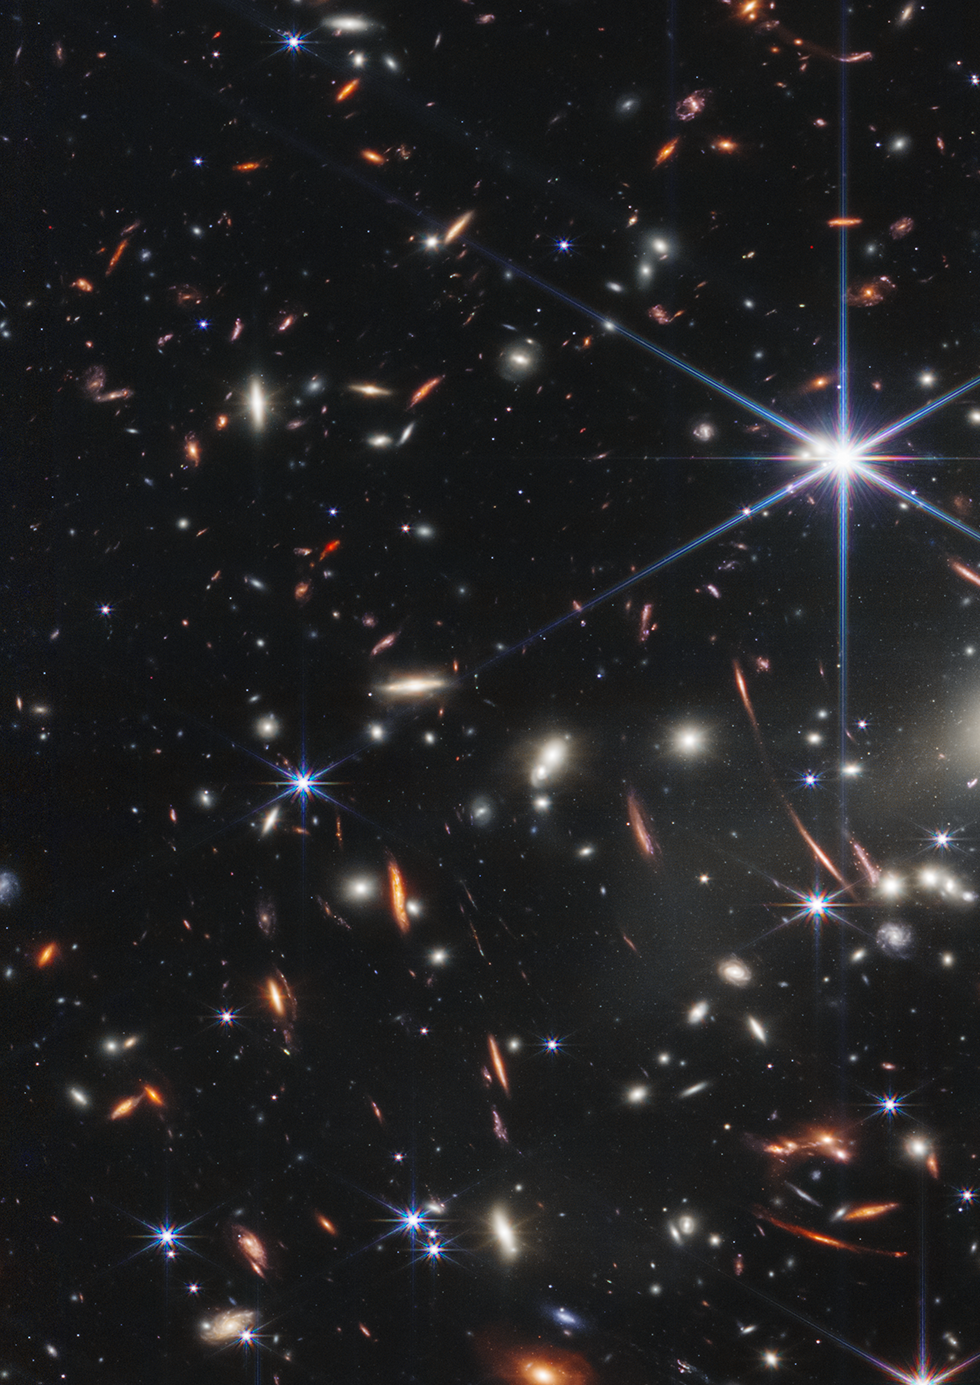
\includegraphics[width=\paperwidth]{Images/SMACS1}}
    }
    \BgThispage
    
    \fancyfoot[C]{\color{white}\thepage}
    \fancyfoot[L]{\vspace{3.5ex}\tiny\textcolor{white}{Credit: NASA, ESA, CSA, STScI}}
    \clearpage
    \newpage
    
    \renewcommand{\CurrentTitleColor}{\color{white}}
\fi

\chapter[Assessing the sources of reionisation]{Assessing the sources of reionisation \\[2ex]\large{A spectroscopic case study of a 30\texorpdfstring{$\times$}{x} lensed galaxy\\[-1ex]at \texorpdfstring{$z \sim 5$}{z~5} with \texorpdfstring{\lya, \CIV, \MgII, and \NeIII}{\lyatext, CIV, MgII, and [NeIII]}}}
\label{ch:Assessing the sources of reionisation}

\ifsetDraft
\else
    \renewcommand{\CurrentTitleColor}{\color{black}}
    
    \backgroundsetup{
        scale=1,
        color=black,
        opacity=1,
        placement=top,
        angle=0,
        contents={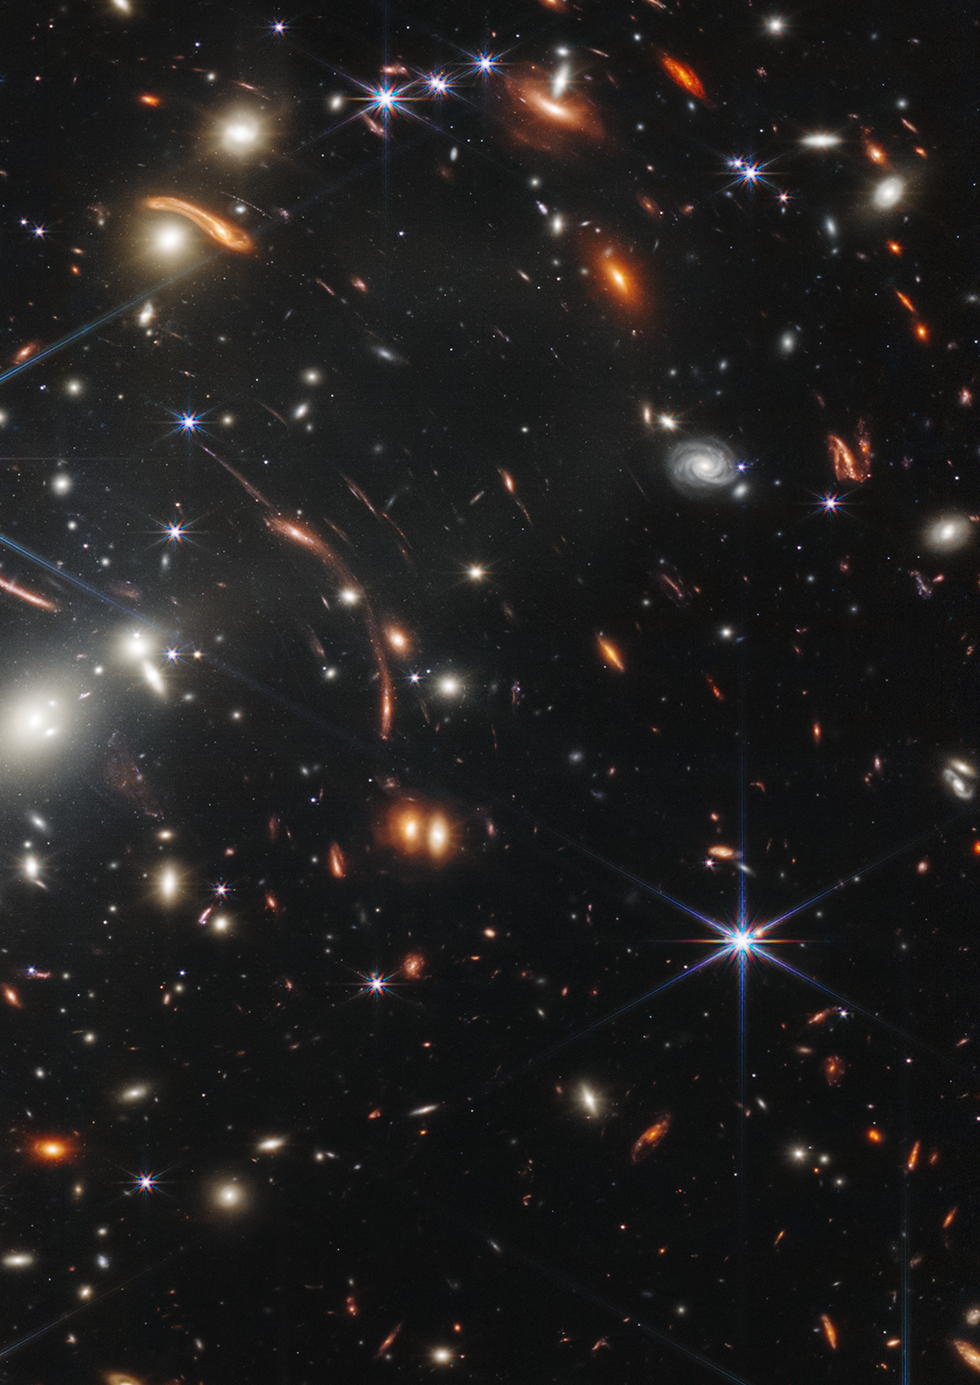
\includegraphics[width=\paperwidth]{Images/SMACS2}}
    }
    \BgThispage
    
    \fancyhf{}
    \fancyfoot[C]{\color{white}\thepage}
    \newpage
    \setFancyHdr
\fi

\section{Introduction}
\label{chAsec:Introduction}

\lettrine{S}{pace-based observatories} such as \textit{HST} and \textit{Spitzer} and ground-based $8 \, \mathrm{m}$-class telescopes have transformed our view of galaxy evolution in the high-redshift Universe, identifying statistically substantial samples of distant galaxies in deep imaging surveys beyond $z>4$ \citep{2014ARA&A..52..415M}. At this epoch, covering the first $\ssim 10\%$ of the current age of the Universe, the physical properties of galaxies were likely to be very different to those today, with metal-poor stellar populations, low stellar masses, and hard radiation fields. These conditions are favourable to strong nebular emission, despite the weak stellar continuum \citep[e.g.][]{2016ARA&A..54..761S}. Equally, this suggests the faint galaxy population in the EoR can contribute significantly to reionisation \citep[e.g.][]{2015ApJ...803...34B}.
\begin{wrapfigure}[12]{R}{0.4\linewidth}
    \begin{mdframed}[backgroundcolor=black!2.5]
        \textsl{This chapter is based on work carried out in collaboration with Renske Smit, Roberto Maiolino, Mirko Curti, Nicolas Laporte, Richard Massey, Johan Richard, and Mark Swinbank. It appeared in MNRAS as \citet*{2021MNRAS.508.1686W}.}
    \end{mdframed}
\end{wrapfigure}

This picture has mainly emerged from spectroscopic follow-up observations of individual distant sources selected in deep photometric surveys, although this poses several challenges. From the ground, NIR spectrometers are restricted by Earth's atmosphere to observe key rest-frame optical emission line features, such as \Halpha, $\OIIIf \, \lambda \, 5008 \, \Angstrom$, and $\OII \, \lambda \, 3727, 3730 \, \Angstrom$ (simply \OII\ hereafter) out to redshifts of about $2.5, 3.6$, and $5.2$, respectively (cf. \cref{chIssec:Observing_galaxies_across_cosmic_time}). The much-anticipated \textit{JWST} will explore the rest-frame optical spectra of more distant objects ($z \sim 4$-$12$), which will enable the use of many emission line diagnostics that are carefully calibrated with the wealth of data for more nearby galaxies, like the optical classification schemes that distinguish spectra of star-forming galaxies shaped by nebular emission from \HII\ regions from those dominated by emission of the narrow-line region of AGN (\cref{chIssec:Nebular_emission_and_emission-line_diagnostics}; see also \citetalias{1981PASP...93....5B}; \citealt{1987ApJS...63..295V}).

Meanwhile, several new methods have been explored, which even as \textit{JWST} is launched will prove valuable in the era of Extremely Large Telescopes (i.e. ELT, GMT, and TMT). For example, alternative classification schemes to the \citetalias{1981PASP...93....5B} classification have been proposed, targeting the rest-frame UV instead: these use highly ionised gas lines such as $\CIIIs \, \lambda \, 1907 \, \Angstrom, \CIIIf \, \lambda \, 1909 \, \Angstrom$ (\CIII\ collectively), $\CIV \, \lambda \, 1548, 1551 \, \Angstrom$ (\CIV), and $\HeII \, \lambda \, 1640 \, \Angstrom$ (\HeII) to separate star-forming galaxies from AGN \citep[e.g.][]{2016MNRAS.456.3354F}. These lines are much brighter in the composite spectra of $z \sim 3$ LBGs than observed in the local Universe \citep[e.g.][]{2003ApJ...588...65S}. Another pressing challenge is to find a reliable method to uncover the sources responsible for reionisation by indirectly identifying LyC leakage in the EoR, where LyC and \ion{H}{I} \lya\ becomes inaccessible due to absorption by the neutral IGM (\cref{chIssec:Epoch_of_Reionisation}). Methods aimed at characterising EoR galaxies, such as the UV classification schemes and indirect proxies of LyC escape, can be tested at (slightly) lower redshift where features are readily observable with current instrumentation, ideally with analogues of high-redshift galaxies.

In this chapter, we present one such case study, investigating in detail the emission line properties of RCS0224z5, a strongly lensed galaxy at redshift $z \simeq 4.88$ in the background of the RCS~0224--0002 cluster. RCS~0224--0002, a galaxy cluster at $z=0.773$, was discovered in the Red-Sequence Cluster Survey \citep[RCS;][]{2002AJ....123....1G}. Several arc-like structures were found in this study, among which an arc consisting of four images of a gravitationally lensed background galaxy at $z \simeq 4.88$, identified via its \lya\ emission. The magnification of the four images ranges from $\mu = 1.30$ to $\mu \sim 140$, making this only one of three known sources at $z \gtrsim 5$ with a comparably high magnification \citep{1997ApJ...486L..75F, 2009MNRAS.400.1121S, 2021ApJ...906..107K} -- and placing this galaxy at less than $300 \, \mathrm{Myr}$ after the end of reionisation. Follow-up observations with VLT/MUSE have furthermore revealed spatially widespread and narrow ($\text{FWHM} \simeq 156 \, \mathrm{km/s}$) \CIV\ emission with a high EW of $\ssim 10 \, \Angstrom$ in the rest frame \citep{2017MNRAS.467.3306S}, similar to what is being observed in an increasing number of $z \sim 6$-$8$ galaxies \citep{2015MNRAS.454.1393S, 2017ApJ...836L..14M, 2017ApJ...851...40L}, but rarely seen in the local Universe \citep{2019ApJ...874...93B, 2019MNRAS.488.3492S}.

We present new VLT/X-shooter observations that constrain the rest-frame UV emission line diagnostics that are inaccessible within the MUSE wavelength range. Unlike sources at higher redshift, where no rest-frame optical features are accessible from the ground, \citet{2007MNRAS.376..479S} presented widespread \OII\ detected in deep SINFONI observations. We present the additional detection of $\NeIII \, \lambda \, 3870 \, \Angstrom$ emission and corresponding new measurement of the \NeIII/\OII\ line diagnostic to place this system in the context of the local galaxy population, in order to gain insight into the origin of high-EW \CIV\ emission in the early Universe. Finally, we report the detection of $\MgII \, \lambda \, 2796 \, \Angstrom$ in emission: a remarkable finding, as this is in stark contrast with the local galaxy population, where it is mostly observed in absorption \citep[e.g.][]{1993ApJS...86....5K}. Being a resonant transition like \lya, it has the potential to be an indirect tracer of LyC escape \citep[e.g.][]{2018ApJ...855...96H}.

The outline of this paper is as follows. In \cref{chAsec:Observations}, we describe the observations, and in \cref{chAsec:Results} we present the results. In \cref{chAsec:Discussion} we discuss the outcomes, and we finally summarise our findings in \cref{chAsec:Summary}. In our analysis, we adopt the cosmological parameters $\Omega_{\text{m}, \, 0} = 0.3$, $\Omega_{\Lambda, \, 0} = 0.7$, and $H_0 = 70 \, \mathrm{km \, s^{-1} \, Mpc^{-1}}$ throughout (implying an angular scale of $6.4 \, \mathrm{kpc/arcsec}$ at $z=4.88$), to ease comparison with previous studies. All magnitudes are in the AB system \citep{1983ApJ...266..713O}.
\begin{figure}
    \centering
    \includegraphics[width=\linewidth]{"Plots/ChapterA/Overview_panel"}
    \caption[Overview of the observations discussed in \cref{chAssec:Observations: X-shooter,chAssec:Observations: SINFONI,chAssec:Observations: HST}]{Overview of the observations discussed in \cref{chAssec:Observations: X-shooter,chAssec:Observations: SINFONI,chAssec:Observations: HST}. \textit{Top left}: \textit{HST} false-colour $I_{814}$, $J_{125}$, and $H_{160}$ image of RCS~0224--0002, indicating the lensed galaxy images 1$-$4 and the FoV of the observations covering the arc of RCS0224z5. \textit{Top right}: \OII\ and \NeIII\ in both X-shooter and SINFONI spectra. \textit{Bottom row}: spectra of \lya, \CIV, and \MgII\ emission lines observed with VLT/X-shooter. An arrow marks a tentative $\ssim 3 \sigma$ redshifted component of \CIV, see \cref{chAssec:Results: X-shooter}. In two-dimensional X-shooter spectra, the dark-light-dark signature of detected lines are highlighted with coloured ellipses (\cref{chAssec:Observations: X-shooter}). Labels indicate the significance of each detection measured in a SNR-optimised aperture (larger for \lya, smaller for \CIV\ and \MgII), while all one-dimensional spectra shown are extracted from a larger aperture to capture the entire flux as reported in \cref{chAtab:Results} (see \cref{chAssec:Results: X-shooter} for details). The grey filled-in area shows the $1 \sigma$ uncertainty level. The rest-frame UV continuum fit is shown with a blue line. Velocities are based on the corresponding systemic redshift of \OII\ (\cref{chAsec:Results}) and are centred on the brightest line for doublets.
    }
    \label{chAfig:Overview panel}
\end{figure}

\section{Observations}
\label{chAsec:Observations}

\begin{table}
    \centering
    \caption[Observational results]
    {Overview of the observed emission lines in the X-shooter and SINFONI spectra. For non-detections, upper limits are given (see \cref{chAssec:Results: X-shooter} for details).
    }
    \begin{tabular}{lcccccc}
        \hline
        Instrument & Image(s)$^a$ & Feature & $\lambda_\text{vac} \, (\Angstrom)^b$ & $\Delta v \, (\mathrm{km/s})^c$ & $\mathrm{Flux}^d \, (10^{-18}$ & $\mathrm{EW} \, (\Angstrom)^e$
        \\
         & & & & & $\mathrm{erg \, s^{-1} \, cm^{-2}})$ &
        \\
        \hline
        \csvreader[late after line=\\, head to column names]{Tables/ChapterA/XResults.csv}{}{\csviffirstrow{\textit{X-shooter} & 1 &}{&&}
            \eline & \wl & \ifcsvstrcmp{\dv}{nan}{\dots}{$\dv \ifcsvstrcmp{\dverr}{nan}{}{\pm \dverr}$} & \ifcsvstrcmp{\flux}{nan}{\dots}{\ifcsvstrcmp{\uplim}{True}{$<\flux$}{$\flux \pm \fluxerr$}} & \ifcsvstrcmp{\EW}{nan}{\dots}{\ifcsvstrcmp{\uplim}{True}{$<\EW$}{$\EW \pm \EWerr$}}
        }
        \hline
        \csvreader[late after line=\\, head to column names]{Tables/ChapterA/SResults.csv}{}{\csviffirstrow{\textit{SINFONI} & 2 and 3 &}{&&}
            \eline & \wl & \ifcsvstrcmp{\dv}{nan}{\dots}{$\dv \ifcsvstrcmp{\dverr}{nan}{}{\pm \dverr}$} & \ifcsvstrcmp{\flux}{nan}{\dots}{\ifcsvstrcmp{\uplim}{True}{$<\flux$}{$\flux \pm \fluxerr$}} & \ifcsvstrcmp{\EW}{nan}{\dots}{\ifcsvstrcmp{\uplim}{True}{$<\EW$}{$\EW \pm \EWerr$}}
        }
    \end{tabular}
    \flushleft
    $^a$ Lensed image(s) from which the spectroscopic measurements were taken (see \cref{chAssec:Observations: X-shooter,chAssec:Observations: SINFONI} for details).
    \\
    $^b$ Vacuum rest-frame wavelength.
    \\
    $^c$ Velocity offset with respect to the systemic redshift as measured by the relevant instrument (X-shooter: $z_\text{sys} = 4.8737$, SINFONI: $z_\text{sys} = 4.8754$). Uncertainty in the velocity offsets includes the uncertainty in determining the systemic redshift (see \cref{chAsec:Results}).
    \\
    $^d$ Observed fluxes, uncorrected for the lensing magnification factor of $\mu = 29_{-11}^{+9}$ of image 1, observed by X-shooter (\cref{chAssec:Observations: X-shooter}), and $\mu = 21_{-8}^{+12}$ and $\mu = 138_{-74}^{+7}$ of image 2 and 3 respectively, observed collectively by SINFONI (\cref{chAssec:Observations: SINFONI}).
    \\
    $^e$ Rest-frame equivalent width (EW; positive values indicating a feature is observed in emission). Note that EWs are independent of lensing magnification.
    \\
    $^f$ Upper limits inferred under the assumption of a minimum ratio of $F_{1907}/F_{1909} \approx 1.39$ for $n_e \leq 10^3 \, \mathrm{cm^{-3}}$ (see \cref{chAssec:Results: X-shooter}).
    \label{chAtab:Results}
\end{table}

\subsection{X-shooter spectroscopy}
\label{chAssec:Observations: X-shooter}

Observations of the lensed image 1 of RCS0224z5, amplified by $\mu = 29_{-11}^{+9}$ \citep[luminosity-weighted; see][]{2017MNRAS.467.3306S}, were taken with the VLT/X-shooter \citep{2011A&A...536A.105V} on 11, 14, and 16 October 2018 with a total on-source time of $3.5 \, \mathrm{h}$, under ESO programme ID 0102.A-0704(A) (PI: Smit); the slit was centred at $\alpha = 02$:24:33.83, $\delta = -00$:02:17.91 (\cref{chAfig:Overview panel}) and using slit widths of $1.2 \arcsec$ and $0.9 \arcsec$ in the visible (VIS) and NIR, resulting in a spectral resolution $R \equiv \lambda/\Delta \lambda \approx 6500$ and $R \approx 5600$, respectively, in the two arms. Observations were taken with AB nodding with an offset of $3.8 \arcsec$ and individual exposures were $383 \, \mathrm{s}$ in the VIS and $230 \, \mathrm{s}$ NIR arm. Observations were taken with an average airmass of $1.14$ and seeing of $0.8 \arcsec$. Data reduction was performed using the standard \program{esoreflex} X-shooter pipeline \citep{2013A&A...559A..96F}. We apply the nodding-mode reduction, as well as stare-mode reduction with a manual algorithm to combine frames from the ``ABBA'' nodding pattern, depending on which yields the best results; the manual stare-mode reduction is used throughout, except for the \CIV\ line. Individual observing blocks (OBs) were separately corrected for telluric absorption in the VIS and NIR arms using \program{molecfit} \citep{2015A&A...576A..77S, 2015A&A...576A..78K}.

\subsection{SINFONI spectroscopy}
\label{chAssec:Observations: SINFONI}

Reduction of the SINFONI IFU spectroscopy is described in \citet{2007MNRAS.376..479S}. In short, IFU spectroscopy was performed for a total of $12 \, \mathrm{h}$ on source with VLT/SINFONI \citep{2003SPIE.4841.1548E, 2004Msngr.117...17B} under ESO programme ID 075.B-0636(B). The data were taken in the HK grating, resulting in a spectral resolution of $R \approx 1700$, with a $\ssim 8 \times 8 \, \mathrm{arcsec^2}$ field of view (at a spatial sampling of $0.25 \, \mathrm{arcsec/pixel}$), covering the lensed images 2 and 3 of RCS0224z5 (luminosity-weighted amplifications of $\mu = 21_{-8}^{+12}$ and $\mu = 138_{-74}^{+7}$, respectively; \citealt{2017MNRAS.467.3306S}). Lensed image 3 has a particularly high amplification (and corresponding uncertainty), as the arc crosses the lensing critical curve. We note that the source plane image of the galaxy is fully recovered by lensed image 1, but only partially in images 2 and 3: out of the two clumps seen in image 1, the one in north east is not reproduced in 2 and 3 \citep[see][ for details]{2017MNRAS.467.3306S}.

\subsection{\textit{HST} imaging}
\label{chAssec:Observations: HST}

\textit{HST} imaging of RCS~0224--0002 is available on the Space Telescope Science Institute data archive\footnote{Data may be obtained from the MAST at \href{https://dx.doi.org/10.17909/t9-9kg5-hg27}{10.17909/T9-9KG5-HG27}.} \citep[GO 14497, PI: Smit; see][]{2017MNRAS.467.3306S}. Observations were performed with the Advanced Camera for Surveys (ACS) using the F814W ($I_{814}$) filter ($2.2 \, \mathrm{ks}$ exposure), and with the Wide Field Camera 3 (WFC3) using the F125W ($J_{125}$) and F160W ($H_{160}$) filters (both $2.6 \, \mathrm{ks}$ exposures). The resulting images reach a depth of $26.3 \, \mathrm{mag}$, $26.8 \, \mathrm{mag}$, and $26.7 \, \mathrm{mag}$ in the $I_{814}$, $J_{125}$, and $H_{160}$ bands ($5\sigma$ for a $0.5 \arcsec$-diameter aperture). A false-colour image of these three bands is shown in the bottom left of \cref{chAfig:Overview panel}.

\section{Results}
\label{chAsec:Results}

In this study, we are mainly interested in line diagnostics using \lya, \CIV, \HeII, the \CIII\ doublet, $\MgII \, \lambda \, 2796, 2804 \, \Angstrom$ (\MgII), \OII, and $\NeIII \, \lambda \, 3870 \, \Angstrom$ (\NeIII).\footnote{In this chapter, we use vacuum wavelengths throughout (see \cref{chAtab:Results}); emission line labels reflect vacuum wavelengths, rounded to the nearest integer.} The measured velocity offsets, line fluxes, and rest-frame EWs (or upper limits) of these lines presented in \cref{chAfig:Overview panel} are summarised in \cref{chAtab:Results}. In the following paragraphs, we will discuss the results for the X-shooter and SINFONI data sets individually.

We derive the systemic redshift from the $\OII \, \lambda \, 3727, 3730 \, \Angstrom$ doublet in combination with the $\NeIII \, \lambda \, 3870 \, \Angstrom$ line for increased precision; for X-shooter, this is measured to be $z_\text{sys} = 4.8737 \pm 0.0010$ (uncorrected for a negligible barycentric velocity of $5$-$7 \, \mathrm{km/s}$), while for SINFONI it is $z_\text{sys} = 4.8754 \pm 0.0003$ (again not corrected for a barycentric velocity of up to $27 \, \mathrm{km/s}$ or $\Delta z = 0.0005$, but consistent with $z_\OII = 4.8757 \pm 0.0005$ measured by \citealt{2007MNRAS.376..479S}), leaving a difference of $\Delta z = 0.0017$. In both cases, we simultaneously fit the \OII\ and \NeIII\ lines while fixing the \OII\ line ratio, due to limited spectral resolution and signal to noise. We adopt a ratio of $F_{3730}/F_{3727} = 1.18$, the median of $z \sim 2.3$ star-forming galaxies reported by \citet{2016ApJ...816...23S}, corresponding to an electron density $\ssim 10^2 \, \mathrm{cm^{-3}}$. Importantly, the \OII\ flux, and hence the \NeIII/\OII\ line ratio, are practically invariant when fitting with a freely varying \OII\ line ratio. For X-shooter, the fit was performed on spectra rebinned to $150 \, \mathrm{km/s}$ and $75 \, \mathrm{km/s}$ for \OII\ and \NeIII\ respectively, using the intrinsic line widths obtained from the fit to the SINFONI spectrum. The $\ssim 2 \sigma$ discrepancy between the systemic redshifts determined by X-shooter and SINFONI, equivalent to $88 \pm 52 \, \mathrm{km/s}$, may be a calibration problem (exceeding barycentric velocity corrections); or, given that the two spectra probe different images (see \cref{chAfig:Overview panel}), the velocity difference can be a consequence of real kinematic differences between the two components. In the following, we measure offsets from the systemic redshift using the consistent measurement in the same image, and by the same instrument. We include the uncertainty in determining the systemic redshift (i.e. $52 \, \mathrm{km/s}$ for X-shooter) in the uncertainty on all velocity offsets.

For all line flux measurements, we fit Gaussian profiles to the one-dimensional spectra. The uncertainty is estimated by scaling the flux uncertainty of a single spectral channel, $F_\lambda \, \Delta \lambda$, by the square root of the number of spectral bins where line flux is detected (coloured channels in \cref{chAfig:Overview panel}).

\subsection{X-shooter}
\label{chAssec:Results: X-shooter}

The relevant X-shooter data are presented in the bottom row of \cref{chAfig:Overview panel}, which shows one-dimensional spectra extracted from a $2.4 \arcsec$ aperture for all lines except \lya, where we use a $3.2 \arcsec$ aperture. These spectra are used to measure the velocity offsets and total fluxes (\cref{chAtab:Results}). The annotated labels show the signal-to-noise ratio (SNR) measured in a smaller $1.4 \arcsec$ aperture, again except for \lya\ where the extended aperture yields a higher SNR. We detect strong \lya\ emission (at $\ssim 80 \sigma$ in a $3.2 \arcsec$ aperture or $\ssim 50 \sigma$ in a $1.4 \arcsec$ aperture; in the $1.4 \arcsec$ aperture, the \lya\ EW decreases to $78 \, \Angstrom$), as well as the \CIV\ doublet, at $8.4 \sigma$ and $4.4 \sigma$. Finally, we detect the $\MgII \, \lambda \, 2796 \, \Angstrom$ line at $5.2 \sigma$ (see \cref{appAsec:MgII and CIII significance} for more details on the significance of this detection). This makes RCS0224z5 the highest redshift galaxy for which \MgII\ emission has been detected. After \lya, the $\MgII \, \lambda \, 2796 \, \Angstrom$ line has the highest EW out of all emission features detected in the rest-frame UV, even though the other line of the doublet, $\MgII \, \lambda \, 2804 \, \Angstrom$, is undetected due to skylines. We show the expected signal for $\MgII \, \lambda \, 2804 \, \Angstrom$ in \cref{chAfig:Overview panel} assuming a typical flux ratio of $F_{2796}/F_{2804} \approx 1.9$ between the $\MgII$ lines at $2796 \, \Angstrom$ and $2804 \, \Angstrom$ \citep[e.g.][]{2018ApJ...855...96H}, which is indeed below the estimated uncertainty level.

The blue line in the \CIV\ doublet, $\CIV \, \lambda \, 1551 \, \Angstrom$, appears to have a weak second redshifted component ($\ssim 3 \sigma$), although the negative signature in the two-dimensional spectrum seems mostly absent, which is why we do not include it in our analysis. At the current sensitivity and spectral resolution, we cannot confidently explain the nature of this feature; however, note that if this emission feature is included in the \CIV\ flux and EW, this would not affect our conclusions in \cref{chAssec:Discussion: CIV} regarding the origin of highly ionised emission.

With X-shooter, we detect the \OII\ doublet and \NeIII\ at $2.2 \sigma$ and $1.8 \sigma$ by rebinning to $150 \, \mathrm{km/s}$ and $75 \, \mathrm{km/s}$, respectively (both in a $1.4 \arcsec$ aperture to maximise SNR). In our analysis, however, we will adopt the measurements of SINFONI at higher significance (see \cref{chAssec:Results: SINFONI}). Furthermore, as shown in \cref{chAtab:Results}, we obtain upper limits on emission from the \HeII\ line and the \CIII\ doublet. Since both lines of the \CIII\ doublet fall directly on skylines, instead of a $2\sigma$ limit from the noise as for \HeII, we take the integrated flux measured within $-100 \, \mathrm{km/s} < v < 100 \, \mathrm{km/s}$ of the expected line centre of the $1907 \, \Angstrom$ line (which is slightly less affected by telluric absorption and skylines; see also \cref{appAsec:MgII and CIII significance}). We obtain an upper limit for the total flux of the doublet using the lowest physically attainable value of $F_{1907}/F_{1909} \approx 1.39$ for $n_e \leq 10^3 \, \mathrm{cm^{-3}}$ \citep{2019ApJ...880...16K}. If we take a ratio of $\ssim 0.34$ for $n_e \leq 10^5 \, \mathrm{cm^{-3}}$, the resulting \CIV/\CIII\ ratio we measure shifts by $0.36 \, \mathrm{dex}$, leaving our findings unaffected (\cref{chAssec:Discussion: CIV}). The $\OIIIs \, \lambda \, 1661, 1666 \, \Angstrom$ doublet also remains undetected: the brightest line of the two, at $1666 \, \Angstrom$, falls on a skyline, and the second line at $1661 \, \Angstrom$ is too faint to provide useful upper limits on the doublet.

By rebinning to a lower spectral resolution (in bins of $\Delta \lambda_\text{obs} = 200 \, \Angstrom$, masking skylines prior to rebinning), we detect the rest-frame UV continuum and assuming $F_\lambda \propto \lambda^\beta_\text{UV}$, we measure a UV-continuum slope $\beta_\text{UV} = -2.36 \pm 0.28$, in good agreement with $\beta_\text{UV} = -2.19 \pm 0.14$ as measured from the \textit{HST} $J_{125} - H_{160}$ colour \citep{2017MNRAS.467.3306S}. This continuum fit is shown in all X-shooter spectra in \cref{chAfig:Overview panel} with a blue line. Using this fit, we deduce the equivalent widths (or upper limits thereof) of observed lines.

\subsection{SINFONI}
\label{chAssec:Results: SINFONI}

In addition to the previously reported observation of the \OII\ doublet with SINFONI \citep[\OII;][]{2007MNRAS.376..479S}, at $13.5 \sigma$ and $15.9 \sigma$ respectively, we present a new $4.8 \sigma$ detection of the \NeIII\ line (see \cref{chAfig:Overview panel}), the highest redshift detection of this line to date. The \NeIII\ feature is not confidently detected with X-shooter, likely due to the shorter exposure time ($3.5 \, \mathrm{h}$ versus $12 \, \mathrm{h}$).

Conversely, even though the SINFONI observations cover the wavelength of \MgII, it was not detected due to the lower spectral resolution of SINFONI ($R \approx 1700$ or $\Delta \lambda_\text{obs} \approx 10 \, \Angstrom$ at the observed wavelength of \MgII, $16426 \, \Angstrom$)\ blending the signal with the strong skyline feature at $16435 \, \Angstrom$.

\section{Discussion}
\label{chAsec:Discussion}
\begin{figure}
    \centering
    \includegraphics[width=0.6\linewidth]{"Plots/ChapterA/Line_ratios_CIV-HeII"}
    \caption[\CIV/\HeII\ line ratio diagnostics]{\textit{Top panel}: line ratio of \CIV/\CIII\ versus \CIV/\HeII. The photoionisation models show predictions for nebular emission \citep[indicated as star-forming or SF; models from][]{2016MNRAS.462.1757G} and narrow-line region AGN emission \citep[models from][]{2016MNRAS.456.3354F}; for both, see the description in the text for details. The black and grey measurements show upper limits on the line ratios for RCS0224z5 assuming a maximum electron density of $n_e \leq 10^3 \, \mathrm{cm^{-3}}$ and $10^5 \, \mathrm{cm^{-3}}$ respectively (shifting the ratio by $0.36 \, \mathrm{dex}$, see \cref{chAssec:Results: X-shooter}), both strongly rejecting AGN model predictions. \textit{Bottom panel}: a UV diagnostic comparison of the rest-frame EW of \CIV\ with the \CIV/\CIII\ ratio \citep[from][]{2019MNRAS.487..333H}. This figure shows RCS0224z5 in comparison to several other extreme line emission galaxies (coloured data points, labelled in the bottom panel's legend): star-forming, high-redshift analogues in the local Universe \citep[; see text for details]{2017MNRAS.472.2608S, 2019ApJ...874...93B}, a LyC-emitting galaxy at $z \sim 3$ \citep{2020MNRAS.491.1093V}, two galaxies at $z \sim 6$ and $7$ shown to be star-forming \citep{2015MNRAS.454.1393S, 2017ApJ...836L..14M}, and a $z \sim 7$ galaxy likely dominated by an AGN \citep{2017ApJ...851...40L}. From these diagnostics, we conclude that there is no strong AGN activity present in RCS0224z5 and the emission is likely produced in star-forming \HII\ regions. Additionally, high-redshift galaxies exhibit \CIV\ EWs that are markedly higher than in any local analogues.}
    \label{chAfig:Line ratios CIV-HeII}
\end{figure}

\subsection{\texorpdfstring{\CIV}{C IV}: driven by star formation or AGN activity?}
\label{chAssec:Discussion: CIV}

The high equivalent width emission of \CIV\ observed in RCS0224z5 ($\ssim 20 \, \Angstrom$) suggests the presence of a source producing ionising photons above the ionisation potential of \CIII, $47.9 \, \mathrm{eV}$ \citep[e.g.][]{2019ApJ...878L...3B}, as well as a high production efficiency of LyC photons, $\xi_\text{ion}$ \citep[e.g.][]{2015MNRAS.454.1393S}. In determining the origin of such ionising radiation -- star formation (SF) or AGN activity -- comparisons between observations and predictions from photoionisation models (e.g. \program{Cloudy}, see \citealt{2013RMxAA..49..137F}; \program{MAPPINGS}, see \citealt{2013ApJS..208...10D}) are now widely used \citep[e.g.][; \citetalias{2019A&ARv..27....3M}]{2001ApJ...556..121K, 2016MNRAS.462.1757G, 2016MNRAS.456.3354F}.

\cref{chAfig:Line ratios CIV-HeII} examines the origin of the hard radiation field in RCS0224z5 with our constraints on the rest-frame UV line fluxes. The top panel of \cref{chAfig:Line ratios CIV-HeII} shows the \CIV/\CIII\ and \CIV/\HeII\ line ratios \citep[a SF versus AGN diagnostic proposed by ][]{2016MNRAS.456.3354F}. We place lower limits on both ratios using the \CIV\ detection and upper limits on \CIII\ and \HeII. For comparison we show grids and lines for modelled nebular emission and narrow-line region AGN emission coloured according to their metallicity \citep[see legend; assuming a solar metallicity of $Z_\odot = 0.01524$,][]{2012MNRAS.427..127B}. The SF models are from \citet{2016MNRAS.462.1757G}, which are based on the latest version of the \citet{2003MNRAS.344.1000B} stellar population synthesis models, while the AGN models are drawn from \citet{2016MNRAS.456.3354F}. All models have a fixed hydrogen density ($n_\text{H}$; in this case $10^3 \, \mathrm{cm^{-3}}$ for AGN and $10^2 \, \mathrm{cm^{-3}}$ for SF models) and dust-to-heavy-element mass ratio (here, $\xi_\text{d}=0.3$). The SF models are shown for different values of ionisation parameter $U$, $\log_{10} U \in \left\{-4, -3, -2, -1 \right\}$, while the grids of narrow-line region AGN emission shown also have a varying $\alpha$ (ranging from $-2.0$ to $-1.2$), the power-law index of the specific luminosity $S_\nu \propto \nu^\alpha$ at rest-frame UV wavelengths, $\lambda_\text{emit} \leq 2500 \, \Angstrom$. We note that the results do not change significantly under different combinations of parameters $n_\text{H}$, $\xi_\text{d}$. The same is true for our assumption about the maximum electron density to establish the \CIII\ doublet flux (see \cref{chAssec:Results: X-shooter}), as shown by the light grey measurement (reflecting a maximum of $n_e \leq 10^5 \, \mathrm{cm^{-3}}$ instead of $10^3 \, \mathrm{cm^{-3}}$; see \cref{chAssec:Results: X-shooter}).

A confirmed LyC-emitting galaxy at $z \simeq 3.21$, Ion2, is shown for comparison \citep{2016A&A...585A..51D, 2016ApJ...825...41V, 2020MNRAS.491.1093V}; interestingly, its line ratios indicate a composite nature even though its spectral features in the UV have been attributed to young, massive stars \citep{2020MNRAS.491.1093V}. Also shown are two additional galaxies, at redshifts $6.11$ \citep{2015MNRAS.454.1393S} and $7.045$ \citep{2017ApJ...836L..14M} which are presumably similar to RCS0224z5, with low mass and a hard ionising radiation field found to be more likely originating from a metal-poor stellar population instead of an AGN. For these galaxies, and for RCS0224z5, the $2 \sigma$ upper limits strongly reject all possibilities of pure AGN models.

The photoionisation models by \citet{2016MNRAS.462.1757G} and \citet{2016MNRAS.456.3354F} are coupled to cosmological simulations by \citet{2019MNRAS.487..333H} to design \citetalias{1981PASP...93....5B}-like UV diagnostics to differentiate star-forming galaxies from AGN. These diagnostics are specifically designed to provide an accurate classification over a wide range of redshifts ($0 < z \lesssim 6$). Their diagnostic mapping the EW of \CIV\ against the \CIV/\HeII\ ratio is shown in the bottom panel of \cref{chAfig:Line ratios CIV-HeII}. We compare our measurement with local star-forming galaxies with extreme emission lines, that can therefore be seen as analogues of high-redshift galaxies: a sample selected through $\HeII \, \lambda \, 4687 \, \Angstrom$ emission \citep[implying a hard ionising spectrum; see][]{2017MNRAS.472.2608S}, and a sample of galaxies selected for high-EW $\OIIIf \, \lambda \, 5008 \, \Angstrom$ emission \citep[among other criteria;][]{2019ApJ...874...93B}. We show the high-redshift star-forming galaxies and mentioned above and, in contrast, a $z = 7.149$ galaxy showing evidence for AGN activity \citep{2017ApJ...851...40L}. The constraints on these high-redshift galaxies are in agreement with respectively the star formation and AGN models. However, there is a noticeable difference in their line ratios relative to the combined sample of low-redshift ``analogues''.

From these diagnostics, we conclude that there is no strong AGN activity present in RCS0224z5 and the emission is likely produced in \HII\ regions. This finding agrees with \citet{2017MNRAS.467.3306S}, who concluded that the \CIV\ emission is likely nebular in origin, based on the ``clumpy'' \CIV\ morphology (as opposed to centrally concentrated emission). Instead, a young ($1$-$3 \, \mathrm{Myr}$), metal-poor stellar population likely has to account for the hard radiation field required for the \CIV\ emission, providing a considerable contribution of photons reaching energies of at least $47.9 \, \mathrm{eV}$. This fits into the picture of the prevalence of extreme line emitters in the early Universe -- both more common and more extreme than any known local analogues -- and accompanying hard radiation fields that has emerged recently \citep[e.g.][]{2014ApJ...784...58S, 2015ApJ...801..122S, 2015MNRAS.454.1393S, 2017ApJ...836L..14M, 2019ApJ...879...70H}.

\subsection{The \texorpdfstring{\NeIII/\OII}{[Ne III]/[O II]} line ratio as an ionisation and metallicity diagnostic alternative to \texorpdfstring{\OIIIf/\OII}{[O III]/[O II]}}
\label{chAssec:Discussion: NeIII/OII}

Neon is an $\upalpha$ element, produced by heavy stars ($M \gtrsim 8 \, \mathrm{M_\odot}$) in their carbon burning cycle and ultimately type-II supernovae, and therefore tightly matches oxygen in abundance \citepalias[][, and references therein]{2019A&ARv..27....3M}. Moreover, \NeIII\ and its isoelectronic equivalent $\OIIIf \, \lambda \, 5008 \, \Angstrom$ (\OIIIf) have a similarly high ionisation potential ($41.0$ and $35.1 \, \mathrm{eV}$, respectively), meaning the luminosity ratio of \NeIII\ and the low-ionisation $\OII \, \lambda \, 3727, 3730 \, \Angstrom$ doublet (\OII) is a powerful diagnostic of the ionisation parameter, similar to \OIIIf/\OII\ \citep[][; \citetalias{2019A&ARv..27....3M}]{2007MNRAS.381..125P, 2014ApJ...780..100L}. The observed relationship between metallicity and ionisation parameter also makes it a metallicity diagnostic, albeit indirectly \citep[causing it to exhibit a significant amount of scatter; see][]{2006A&A...459...85N, 2008A&A...488..463M}: metal-poor systems are expected to have a high \NeIII/\OII\ ratio.

The fact that \NeIII\ and \OII\ have both similar and short wavelengths gives the \NeIII/\OII\ diagnostic two distinct advantages over the widely used \OIIIf/\OII\ ratio: it is practically insensitive to dust attenuation, and it can be detected at higher redshifts with ground-based near-infrared instruments \citep{2014ApJ...780..100L}. The former has long been exploited \citep[e.g.][]{2002ApJ...581..205H}, and indeed, \NeIII\ has been detected several times at $z \gtrsim 3$, in combination with \OII: in particular, we will consider here the galaxies Ion2 at $z \simeq 3.21$, a confirmed LyC-emitting galaxy \citep[as discussed in \cref{chAssec:Discussion: CIV};][]{2016A&A...585A..51D, 2016ApJ...825...41V, 2020MNRAS.491.1093V}, SMACS~J2031.8-4036 at $z \simeq 3.51$ \citep{2012MNRAS.427.1953C, 2012MNRAS.427.1973C, 2016MNRAS.456.4191P}, GOODSN-17940 at $z \simeq 4.41$ \citep{2017ApJ...846L..30S}, and LnA1689-2 at $z \simeq 4.87$ \citep{2014A&A...563A..58T}.

\begin{figure}
    \centering
    \includegraphics[width=0.6\linewidth]{"Plots/ChapterA/SDSS_NeIII-OII_M_star_DR7"}
    \caption[Measurements of \NeIII/\OII\ line ratios of local and high-redshift galaxies]{\NeIII/\OII\ ratio of selected SDSS galaxies in bins of stellar mass (star-forming galaxies in blue, Seyfert in purple), as well as measurements of local LyC leakers (\Isample). Binned samples at $z = 2.3$ and $z = 3.3$ from the MOSDEF survey \citep{2021ApJ...914...19S} and the LyC-leaking galaxy Ion2 at $z \simeq 3.21$ \citep{2020MNRAS.491.1093V} are shown as a reference at intermediate redshift. At the very highest redshift for which measurements of \NeIII/\OII\ are currently possible, we include three star-forming galaxies, at $z \simeq 3.51$, $z \simeq 4.41$ and $z \simeq 4.87$ \citep[, respectively; see text]{2012MNRAS.427.1953C, 2017ApJ...846L..30S, 2014A&A...563A..58T}, and RCS0224z5. A tentative trend emerges, spanning nearly two orders of magnitude in the \NeIII/\OII\ ratio. Star-forming galaxies at $z \sim 0$ have a ratio of $\sim 0.01$ (with little scatter), whereas the ratio is significantly increased at higher redshift, $\ssim 0.1$ at $z \sim 2$-$3$. The trend culminates at $z \sim 5$: the ratio of RCS0224z5 ($\ssim 0.6$), seemingly typical based on this trend, is comparable to that of local LyC leakers, which are clear outliers compared to the general $z \sim 0$ galaxy population.
    }
    \label{chAfig:NeIII/OII line ratio vs stellar mass}
\end{figure}

\subsubsection{\texorpdfstring{\NeIII/\OII}{[Ne III]/[O II]} evolution over stellar mass and cosmic time}
\label{chAsssec:NeIII/OII evolution}

The emission line ratio $\NeIII/\OII = 0.46 \pm 0.10$ for RCS0224z5 is shown as a function of stellar mass in \cref{chAfig:NeIII/OII line ratio vs stellar mass}. To find the stellar mass for images 2 and 3 independent of magnification uncertainties, we follow the derivation of \citet{2007MNRAS.376..479S}, who reported a dynamical mass estimate of $M_\text{dyn} \sim 10^{10} \, \mathrm{M}_\odot$ based on the \OII\ velocity dispersion \citep[via equation (1) in][]{2006ApJ...646..107E}. We assume a fiducial $C = 3 \pm 2$ \citep[with high uncertainty to reflect the range of possible values depending on mass distribution and velocity field, see][]{2006ApJ...646..107E}, and our measured \OII\ line width of $\sigma_\OII = 151 \pm 30 \, \mathrm{km/s}$ within $r = 2 \, \mathrm{kpc}$ \citep[following][]{2007MNRAS.376..479S}. We then take the typical stellar mass fraction of $z \sim 1$-$2$ star-forming galaxies of $27 \pm 5\%$, reflecting the range $22$-$32\%$ reported by \citet[; see also \citealt{2016ApJ...831..149W}]{2016MNRAS.457.1888S}, to derive a stellar mass of $(9 \pm 7) \times 10^{9} \, \mathrm{M}_\odot$. We note that with \textit{HST} photometry of image 1 (high magnification uncertainties prevent us from using the incomplete images 2 and 3), we derive a stellar mass of $4_{-3}^{+14} \times 10^8 \, \mathrm{M_\odot}$, using the \program{fast} code \citep[Fitting and Assessment of Synthetic Templates;][]{2009ApJ...700..221K}, assuming a constant SFR, a \citet{2003PASP..115..763C} IMF, a minimum age of $10^7 \, \mathrm{yr}$ (the maximum age equal to the age of the universe at $z = 4.88$), an Small Magellanic Cloud (SMC) dust law, the \citet{2003MNRAS.344.1000B} stellar libraries, and a metallicity of $Z = 0.2 \, \mathrm{Z_\odot}$. This estimate is marginally lower, but consistent within the uncertainty of the stellar mass obtained from the dynamical mass estimate.

Furthermore, the $\mathrm{SFR}_\OII$ of $12 \pm 2 \, \mathrm{M_\odot \, yr^{-1}}$ measured for image 2 and 3 by \citet{2007MNRAS.376..479S} -- combined with the stellar mass estimated from the dynamical mass -- places RCS0224z5 just under on the main sequence at its redshift \citep[e.g.][; a lower stellar mass, as suggested by the SED modelling, would shift it onto the main sequence]{2015ApJ...799..183S}. This supports the hypothesis that RCS0224z5 is a typical $z \sim 5$ star-forming galaxy.

To put our measurements of the near-UV \NeIII\ and \OII\ lines into perspective, we turn to a large observational sample of nearby galaxies from SDSS DR7 \citep{2009ApJS..182..543A}, retrieving line fluxes from the MPA-JHU emission line catalogue for $\num[group-separator={,}]{827640}$ unique sources.\footnote{The catalogue is available at \url{https://www.mpa-garching.mpg.de/SDSS/DR7/}, while a description of the relevant methods used to compile it can be found in \citet{2004ApJ...613..898T}.} A detailed description of the selection procedure for the galaxies used here is given in \cref{appAsec:SDSS selection}. The \NeIII/\OII\ ratio of these nearby galaxies are shown in bins of stellar mass (for bins with at least $25$ galaxies), for the two main classes (star-forming and Seyfert; see \cref{appAsec:SDSS selection}). Additionally, we compare these to local LyC-leaking galaxies; in particular, we will consider a sample compiled from \citet{2016MNRAS.461.3683I, 2016Natur.529..178I, 2018MNRAS.474.4514I, 2018MNRAS.478.4851I, 2020A&A...639A..85G, 2020MNRAS.497.4293G}, together simply the \Isample\ hereafter. Finally, individual measurements of the aforementioned high-redshift galaxies at $z \simeq 3.21, 3.51, 4.41, 4.87$ \citep[, respectively]{2020MNRAS.491.1093V, 2012MNRAS.427.1953C, 2017ApJ...846L..30S, 2014A&A...563A..58T} are shown.

\cref{chAfig:NeIII/OII line ratio vs stellar mass} illustrates that RCS0224z5 has a \NeIII/\OII\ ratio consistent with LyC leakers (both those at low redshift and Ion2 at $z \simeq 3.21$), and nearly two orders of magnitude higher than local star forming galaxies with the same mass. This agrees with recent findings of enhanced \NeIII/\OII\ ratios in star-forming galaxies at $z \sim 2$ \citep{2015ApJ...798...29Z, 2020ApJ...902L..16J}. Moreover, this is in agreement with the expectation that \NeIII/\OII\ is a proxy of \OIIIf/\OII, and that RCS0224z5 might have a high LyC escape fraction, as discussed further below (\cref{chAssec:Discussion: Lya and MgII}).
\begin{figure}
    \centering
    \includegraphics[width=0.6\linewidth]{"Plots/ChapterA/SDSS_NeIII-OII_vs_OIII-OII_DR7"}
    \caption[Correlation between the \NeIII/\OII\ and \OIIIf/\OII\ line ratios of SDSS galaxies]{Correlation between the \NeIII/\OII\ and \OIIIf/\OII\ line ratios of SDSS galaxies (star-forming galaxies in blue, Seyfert in purple). Also shown are Ion2 at $z \simeq 3.21$ \citep{2020MNRAS.491.1093V}, SMACS~J2031.8-4036 at $z \simeq 3.51$ \citep{2012MNRAS.427.1953C}, the LyC leakers from the \Isample, as well as $6$ extreme ``Green Pea'' galaxies from \citet{2013ApJ...766...91J}. The vertical grey dashed line shows the completeness limit of 90\%, while the fiducial limit ratio of $\OIIIf/\OII \geq 5$ used to characterise LyC leakers is shown by the vertical black dashed line (see text for details on both). Ionisation parameter values of $\log_{10} U = -3, -2$ are indicated by vertical blue lines \citep[see \cref{chAeq:OIII/OII logU diagnostic}, derived by][]{2000MNRAS.318..462D}. Direct measurements of Ion2 and SMACS~J2031.8-4036 suggest the correlation between \NeIII/\OII\ and \OIIIf/\OII\ seen in local galaxies holds well at higher redshift. Both these sources and RCS0224z5, shown by the black line with grey uncertainty, have a high ionisation parameter compared to local galaxies, similar to that of LyC-leaking systems, but may very well be typical examples at high redshift as they do not seem to be as extreme outliers compared to their contemporaries (\cref{chAfig:NeIII/OII line ratio vs stellar mass}).}
    \label{chAfig:NeIII/OII vs OIII/OII line ratios}
\end{figure}

\subsubsection{\texorpdfstring{\NeIII/\OII}{[Ne III]/[O II]} as a proxy for the ionisation state of the ISM}
\label{chAsssec:NeIII/OII as a proxy for the ionisation state of the ISM}

As evidenced by its tight correlation with \OIIIf/\OII\ in local galaxies \citep[e.g.][]{2020ApJ...902L..16J}, the \NeIII/\OII\ ratio is a robust tracer of the ionisation parameter. Previous studies have proved the strong similarity between the \NeIII/\OII\ and \OIIIf/\OII\ ratios theoretically; however, their quantitative predictions did not quite match observations, which is thought to be due to the modelled ionising spectra being insufficiently hard \citep{2014ApJ...780..100L}. We therefore construct an empirical relationship here by exploiting the statistics of SDSS. In \cref{chAfig:NeIII/OII vs OIII/OII line ratios}, the distributions of \NeIII/\OII\ and \OIIIf/\OII\ line ratios are shown for two classes of SDSS galaxies (star-forming and Seyfert; see \cref{appAsec:SDSS selection}). The LyC leakers from the \Isample\ are again shown for comparison, along with six other local galaxies selected for extreme \OIIIf\ emission \citep[``Green Peas'', or GPs;][]{2013ApJ...766...91J}, as well as the high-redshift galaxies Ion2 and SMACS~J2031.8-4036 \citep[, respectively]{2020MNRAS.491.1093V, 2012MNRAS.427.1953C}. The fiducial limiting ratio of $\OIIIf/\OII \geq 5$ used to characterise LyC leakers is shown by a vertical dashed black line.

To fit the relationship from the SDSS sample, we first define the completeness of a given \OIIIf/\OII\ bin to be the fraction of galaxies contained in that bin with a \NeIII\ SNR higher than 5. At values of $\OIIIf/\OII \lesssim 1$, this completeness drops significantly. Since we require a highly significant \OII\ detection ($\text{SNR} > 30$, see \cref{appAsec:SDSS selection}), the uncertainty on the \NeIII/\OII\ ratio is dominated by that of \NeIII, explaining the scattered cloud of points in contrast to the tight correlation seen at $\OIIIf/\OII > 1$. As \NeIII\ is the weakest out of the three lines considered here \citepalias{2019A&ARv..27....3M}, we fit the relation taking into account uncertainties on the \NeIII/\OII\ ratio only. For star-forming galaxies we exclude points in the region where the completeness fails to meet $90\%$ ($\OIIIf/\OII < 0.849$; grey dashed line in \cref{chAfig:NeIII/OII vs OIII/OII line ratios}). For the remaining $272$ points, we find a Spearman's rank correlation coefficient (measured in log-log space) of $\rho_\text{S} = 0.87$, indicating a strong positive correlation. Moreover, the resulting fit captures the behaviour at both the low and high \OIIIf/\OII\ ratios well: extrapolating to lower \OIIIf/\OII\ ratios the low-SNR SDSS data are scattered around the relation symmetrically, while extrapolating to higher \OIIIf/\OII\ ratios the extreme ratios of GP galaxies (not included in the fit) are consistent with this trend. The fit for star-forming galaxies is given by
\begin{equation}
    \label{chAeq:NeIII-OII vs OIII/OII correlation}
    \log_{10} \left( \frac{\NeIII}{\OII} \right) = 0.9051 \log_{10} \left( \frac{\OIIIf}{\OII} \right) - 1.078 \, .
\end{equation}

For example, the proposed line ratio above which a significant fraction of sources might be leaking LyC photons, $\OIIIf/\OII \geq 5$, \citep[e.g.][]{2016Natur.529..178I, 2016MNRAS.461.3683I} corresponds to $\NeIII/\OII \geq 0.36$. Furthermore, with this empirical relationship, we can translate diagnostics based on the \OIIIf/\OII\ ratio, e.g. a diagnostic for the ionisation parameter \citep[derived from single-star photoionisation models, see][]{2000MNRAS.318..462D},
\begin{equation}
    \label{chAeq:OIII/OII logU diagnostic}
    \log_{10} U = 0.80 \log_{10} \left( \frac{\OIIIf}{\OII} \right) - 3.02 \, .
\end{equation}

Vertical blue lines indicate values of $\log_{10} U = -3, -2$ in \cref{chAfig:NeIII/OII vs OIII/OII line ratios}. Combining \cref{chAeq:NeIII-OII vs OIII/OII correlation,chAeq:OIII/OII logU diagnostic}, we derive
\begin{align}
    \label{chAeq:NeIII/OII logU diagnostic}
    \log_{10} U & = 0.80 \frac{\log_{10} \left( \NeIII/\OII \right) + 1.078}{0.9051} - 3.02 \nonumber
    \\
    & = 0.884 \log_{10} \left( \frac{\NeIII}{\OII} \right) - 2.07
\end{align}

\noindent In the case of RCS0224z5, we find an ionisation parameter of $\log_{10} U = -2.37 \pm 0.08$. Given its derivation from the \NeIII/\OII\ ratio, we again note this is likely not an extreme case at its redshift \citep[\cref{chAfig:NeIII/OII line ratio vs stellar mass}, and see similar estimates of $U$ at $z \sim 7$-$8$ in][]{2017MNRAS.464..469S}, but a high ionisation parameter compared to local galaxies, similar to that of LyC-leaking systems (the limit of $\OIIIf/\OII \geq 5$ translates to $\log_{10} U = -2.46$).

However, the \NeIII/\OII\ ratio is also an indirect tracer of the gas metallicity (being mostly anticorrelated with metallicity). The fact that RCS0224z5 (along with GOODSN-17940) has \NeIII/\OII\ much higher than local galaxies, and hence much lower metallicity, is also likely linked to the redshift evolution of the mass-metallicity relation (MZR, see \cref{chIssec:Chemical_enrichment}). This is illustrated in \cref{chAfig:NeIII/OII line ratio vs stellar mass} where binned samples are shown at intermediate redshifts, $z = 2.3$ and $z = 3.3$ \citep[measurements from MOSDEF the MOSFIRE Deep Evolution Field survey;][]{2021ApJ...914...19S}. The tentative evolutionary trend of the \NeIII/\OII\ ratio with redshift seen in \cref{chAfig:NeIII/OII line ratio vs stellar mass} has indeed been verified to approximately reproduce the MZR as observed with a variety of metallicity tracers \citep[e.g.][]{2008A&A...488..463M}. The next section will discuss the diagnosticity of \NeIII/\OII\ specifically regarding metallicity in further detail.
\begin{figure}
    \centering
    \includegraphics[width=0.6\linewidth]{"Plots/ChapterA/Delta_FMR"}
    \caption[Offsets from the FMR]{Offsets from the FMR, given by the inferred metallicity minus the one derived from the FMR. Intrinsic uncertainty of the FMR (which varies with both stellar mass and SFR) is indicated by the grey shaded regions, the darker region typical for galaxies at high mass and low SFR, the lighter region for galaxies at low mass and high SFR \citep[for details, see][]{2020MNRAS.491..944C}. At low redshift, the LyC leakers from the \Isample\ are shown. Samples binned by stellar mass at $z = 2.3$ and $z = 3.3$ from the MOSDEF survey \citep{2021ApJ...914...19S} are shown, as well as a binned sample of $31$ galaxies at $z \sim 3$-$4$ from the AMAZE and LSD surveys, presented in \citet{2014A&A...563A..58T}. LnA1689-2 is excluded from the latter and instead shown individually at $z \simeq 4.87$, as are Ion2 at $z \simeq 3.21$ \citep{2020MNRAS.491.1093V}, SMACS~J2031.8-4036 at $z \simeq 3.51$ \citep{2012MNRAS.427.1953C}, GOODSN-17940 at $z \simeq 4.41$ \citep{2017ApJ...846L..30S}. Galaxies at the highest redshift seem to show a trend towards negative differences, i.e. metallicities smaller than expected from the FMR.}
    \label{chAfig:NeIII/OII delta FMR}
\end{figure}

\subsubsection{Tracing metallicity with \texorpdfstring{\NeIII/\OII}{[Ne III]/[O II]}}
\label{chAsssec:Tracing metallicity with NeIII/OII}

By virtue of its correlation with the ionisation parameter, the \NeIII/\OII\ ratio is also an indirect tracer of the metallicity. In the following we discuss the former aspect in greater detail, albeit with the caveat that the ratio is a more robust diagnostic for the ionisation parameter than for metallicity.

By using the metallicity diagnostic relation for \NeIII/\OII\ from \citet{2018ApJ...859..175B}, calibrated with local analogues of high-redshift galaxies, we obtain $12 + \log \left ( \text{O/H} \right) = 8.01_{-0.21}^{+0.21}$ for RCS0224z5, where we have included a $0.2 \, \mathrm{dex}$ systematic calibration uncertainty (see e.g. \citealt{2006A&A...459...85N}). This corresponds to roughly $20\%$ of the solar metallicity: $Z = 0.21_{-0.08}^{+0.13} \, \mathrm{Z_\odot}$.\footnote{We adopt a solar oxygen abundance of $12 + \log \left ( \text{O/H} \right)_\odot = 8.69$ \citep{2009ARA&A..47..481A}.} The galaxies at $z \sim 4$-$5$ with \NeIII\ and \OII\ measurements are clearly characterised by significantly higher line ratios (\cref{chAfig:NeIII/OII line ratio vs stellar mass}), and hence higher ionisation parameters than $z \sim 3.5$ galaxies. Using the (uncertain) strong-line calibration, we can indirectly infer they have lower metallicities too, which would confirm that they do follow the general redshift evolution of metallicity.

However, one should take into account that the metallicity of star-forming galaxies also shows a secondary dependence on SFR that, together with the primary dependence on mass, is dubbed Fundamental Metallicity Relation (FMR, see \cref{chIssec:Chemical_enrichment}; see also \citealt{2010MNRAS.408.2115M}; \citetalias{2019A&ARv..27....3M}). This secondary dependence is thought to result from a more fundamental relation with the gas content \citep{2013MNRAS.433.1425B, 2016MNRAS.455.1156B, 2016A&A...595A..48B} and ascribed primarily to the accretion of near-pristine (or low-metallicity) gas which increases the gas content and dilutes the metallicity; the increased gas content also results into an increased SFR through the \citeauthor{1959ApJ...129..243S}-\citeauthor{1989ApJ...344..685K} relation, which gives the observed anticorrelation between SFR and metallicity. Once this secondary dependence is taken into account then the redshift evolution of the metallicity is essentially absent, at least out to $z \sim 2.5$ \citep{2010MNRAS.408.2115M, 2019A&A...627A..42C}. Some deviation from the FMR was claimed at $z > 3$ \citep{2014A&A...563A..58T}, but more recently \cite{2021ApJ...914...19S} have shown that their sample at z$\sim$3 follows the same FMR as local galaxies if metallicities are measured through the \citet{2018ApJ...859..175B} calibration.

We assess whether RCS0224z5 and other high-redshift galaxies, as well as the local LyC leakers from the \Isample, follow the FMR, carefully revisiting all measurements in a consistent way, as discussed in the following. At high redshift, we consider galaxies at $z > 2$ from \citet{2021ApJ...914...19S} and \citet{2014A&A...563A..58T}, as well as the three galaxies at $z > 4$ with detections of \NeIII\ and \OII\ already discussed in the previous section. For RCS0224z5 we use the stellar mass of images 2 and 3 obtained from the dynamical mass, $(9 \pm 7) \times 10^{9} \, \mathrm{M}_\odot$ (including uncertainties on $C$, the stellar mass fraction, and $\sigma_\OII$, discussed in \cref{chAsssec:NeIII/OII evolution}), and the SFR of images 2 and 3, $12 \pm 2 \, \mathrm{M_\odot \, yr^{-1}}$, as reported by \citet{2007MNRAS.376..479S}. We also include the two individual galaxies at $z \sim 3$ with \NeIII\ and \OII\ measurements discussed in the previous section. We use the same high-redshift calibration from \citet{2018ApJ...859..175B} for all high-redshift galaxies. We then consider $\Delta_\text{FMR} ( 12 + \log ( \text{O/H} ))$, the deviation of the measured metallicity from the local FMR, defined as
\begin{equation}
    \Delta_\text{FMR} \left( 12 + \log \left ( \text{O/H} \right) \right) = 12 + \log \left( \text{O/H} \right) - \left( 12 + \log \left ( \text{O/H} \right) \right)_\text{FMR} \, .
\end{equation}

Here, we describe the metallicity predicted by the local FMR, $( 12 + \log ( \text{O/H} ))_\text{FMR}$, as a function of stellar mass and SFR through equation (5) in \citet{2020MNRAS.491..944C}. The best-fit parameters obtained by \citeauthor{2020MNRAS.491..944C} adopt $T_e$-based metallicity calibrations \citep[as][, but based on the full SDSS dataset]{2018ApJ...859..175B}. Uncertainties are estimated by independently varying the input variables $(M_*, \text{SFR})$ within the $1 \sigma$ uncertainty range and adding the resulting deviations in quadrature. For LyC leakers in the \Isample, we calculate the FMR offset if the metallicity has been reported. We show the resulting deviations from the FMR in \cref{chAfig:NeIII/OII delta FMR}.

While at $z \sim 2$ galaxies are fully consistent with the local FMR, at $z > 3$ galaxies start having a larger scatter and tend to be distributed towards lower metallicities with respect to the FMR, also depending on the sample. Although the uncertainties are large, RCS0224z5 also shows some mild tension with respect to the local FMR, being more metal poor. Interestingly, the nearby LyC-leaking galaxies exhibit a significant offset in a similar direction. The other galaxy at nearly the same redshift, LnA1689-2 from the \citeauthor{2014A&A...563A..58T} sample, likewise deviates from the FMR. Since the FMR is considered a relation describing the smooth evolution of galaxies in near-equilibrium between the inflow and outflow of gas and star formation, these findings may suggest that such young galaxies at $z \sim 5$ are in an early stage of evolution in which they have not yet reached a steady equilibrium as the more evolved galaxies at lower redshifts, possibly as a consequence of an excess in gas accretion, which results in additional dilution of metals. However, these results should be confirmed with a larger sample of galaxies at $z > 4$ and by using additional metallicity diagnostics, which will certainly be feasible with \textit{JWST}.

Finally, we note that the estimated metallicity obtained through the \NeIII/\OII\ ratio is significantly higher than the values required in stellar population synthesis models to reproduce the observed \CIV\ EW ($Z < 0.05 \, \mathrm{Z_\odot}$, as shown in \citealt{2017MNRAS.467.3306S}). This indicates the hardness of the ionising spectrum may currently be underestimated in such models. The lack of ionising photons above $47.9 \, \mathrm{eV}$ could be accounted for by physics currently not captured in models \citep[e.g. stars stripped in binaries,][]{2019A&A...629A.134G}, or it may be explained by a lower stellar iron abundance than derived using the nebular oxygen abundance and assuming solar oxygen-to-iron ratios (O/Fe). A higher oxygen-to-iron is expected in the early Universe compared to local galaxies, given that AGB stars have lifetimes of only a few gigayears and metal enrichment is dominated by supernovae \citepalias{2019A&ARv..27....3M}. In particular, the discrepancy seems to agree well with the findings of \citet{2016ApJ...826..159S}, who demonstrate that the oxygen-to-iron ratio of their sample of star-forming galaxies at $z \sim 2.4$ is elevated by a factor of $\ssim 4$ relative to the solar value (i.e. virtually the same enhancement as the ratio between the metallicities discussed here, $20\%$ and $5\%$ solar). While RCS0224z5 appears moderately metal-enriched as measured indirectly with \NeIII/\OII\ (probing the nebular oxygen abundance), stellar atmospheres could be significantly more iron-poor than expected when assuming a solar O/Fe ratio, resulting in an ionising spectrum sufficiently hard to explain the observed \CIV\ EW.

More generally, these results show the potential of \NeIII\ as a powerful diagnostic, specifically for the study of high-redshift galaxies. Note, however, that the \NeIII\ line can blend with $\ion{He}{I} \, \lambda \, 3890 \, \Angstrom$, separated by $\ssim 1500 \, \mathrm{km/s}$, in low-resolution spectra ($R \lesssim 200$). This effect becomes more prominent when the lines are broadened, for example with a significant contribution from the broad-line region of an AGN \citep[e.g.][]{2017ApJ...846..102M} -- this will not be the case, however, for star-forming systems dominated by narrow nebular emission lines.
\begin{figure}
    \centering
    \includegraphics[width=0.6\linewidth]{"Plots/ChapterA/Lya-MgII_EW_dist"}
    \caption[EWs of \lya\ and $\MgII \, \lambda \, 2796 \, \Angstrom$]{Equivalent widths of \lya\ and $\MgII \, \lambda \, 2796 \, \Angstrom$ of RCS0224z5, compared to local extreme emission line galaxies, among which ten LyC-emitting sources \citep[the \Isample\ and][, coloured according to the escape fraction of LyC, if known]{2018ApJ...855...96H}. The correlation between \lya\ and \MgII\ EWs is one of the indicators that the escape mechanisms of \lya\ and \MgII\ are similar. Moreover, relatively high EWs imply that both \lya\ and \MgII\ escape is comparatively high in RCS0224z5.
    }
    \label{chAfig:Lya-MgII EW distribution}
\end{figure}
\begin{figure}
    \centering
    \includegraphics[width=0.6\linewidth]{"Plots/ChapterA/Lya-MgII_v_offsets_fesc"}
    \caption[Escape fractions compared to velocity offsets of \lya\ and $\MgII \, \lambda \, 2796 \, \Angstrom$]{Escape fractions of \lya\ radiation (top) and $\MgII \, \lambda \, 2796 \, \Angstrom$ (bottom) compared to the corresponding velocity offsets of \lya\ (its red peak; top) and the peak of $\MgII \, \lambda \, 2796 \, \Angstrom$ (bottom), compared to local extreme emission line galaxies. Among these are ten LyC-emitting sources \citep[the \Isample\ and][, coloured according to the escape fraction of LyC, if known]{2018ApJ...855...96H}. In the top panel, a sample of Green Pea galaxies from \citet{2016ApJ...820..130Y, 2017ApJ...844..171Y} is shown (the sample consists of $43$ galaxies, among which $5$ are already contained in the \Isample), with a simple power-law fit. Both panels show a similar trend (though with considerable scatter), where a small velocity offset indicates a large escape fraction. The measured velocity offsets of RCS0224z5 (effectively an upper limit in the case of \lya\ due to IGM absorption) again suggest relatively high escape fractions, which is supported by the predicted escape fraction of $\MgII \, \lambda \, 2796 \, \Angstrom$ (the horizontal dashed line; see text for details).
    }
    \label{chAfig:Lya/LyC-MgII escape and velocity offsets}
\end{figure}

\subsection{LyC escape traced by \texorpdfstring{\lya\ and \MgII}{\lyatext and Mg II} emission}
\label{chAssec:Discussion: Lya and MgII}

\subsubsection{Velocity offsets of \texorpdfstring{\lya}{\lyatext} and \texorpdfstring{\MgII}{Mg II}}
\label{chAsssec:Lya}

Using spatially resolved MUSE spectroscopy, \citet{2017MNRAS.467.3306S} demonstrated the presence of extended, high-EW \lya\ emission, with a narrow, red peak emerging very close to the systemic redshift (defined by \OII), regardless of position within the \lya\ halo. X-shooter has a higher spectral resolution than MUSE at $\ssim 7000 \, \Angstrom$ ($R \sim 6500$ versus $R \sim 2700$, respectively). We fit an asymmetric Gaussian line profile \citep[see e.g.][]{2014ApJ...788...74S} to the \lya\ observed in image 1 by X-shooter (see \cref{chAfig:Overview panel}). We find a velocity offset of $\Delta v_\text{peak} = 156 \pm 52 \, \mathrm{km/s}$ from the systemic redshift \citep[in agreement with][]{2017MNRAS.467.3306S}, FWHM of $207 \pm 6 \, \mathrm{km/s}$, and asymmetry factor $a_\text{asym} = 0.32 \pm 0.01$, indicating a skewed profile with a red wing. The asymmetric Gaussian provides an overall good fit, but does show non-vanishing residuals, particularly at the line peak, as well as the regions around $400$ and $1000 \, \mathrm{km/s}$. As we lack sufficient angular resolution in the spectrum to study the \lya\ line shape in depth, we will not focus on possible interpretations here and instead refer to the extensive discussion in \citet[][]{2017MNRAS.467.3306S}.

The determination of the peak offset can provide interesting constraints on properties of the neutral ISM. In particular, the peak \emph{separation} in a double-peaked \lya\ profile (peak offset being the closest alternative to peak separation in the absence of a blue peak\footnote{The velocity offset of the blue peak actually offers the best predictive power \citep{2017A&A...597A..13V}.} in the observed spectrum as a result of absorption in the intervening neutral IGM) is an indicator of resonant scattering of escaping \lya\ photons: a higher column density of neutral hydrogen along the path of escape means more scattering, affecting the line profile shape to have its peak appear increasingly further from the systemic velocity at which the photons were produced: only photons far away from resonance (in frequency space), with a resulting low cross section, are able to escape \citep[e.g.][]{2017A&A...597A..13V}. In the context of the escape of LyC, which is itself governed by the same distribution of neutral hydrogen, the peak separation has proven to be a solid predictor of LyC escape fractions \citep{2017A&A...597A..13V, 2018MNRAS.478.4851I, 2020A&A...639A..85G}. There are other indirect probes of LyC escape, though, which become necessary for application in the EoR, where \lya\ (including the red peak) can be fully absorbed, as a result of the broad damping wing \citep[e.g.][]{2014PASA...31...40D}. Within this context, \MgII, also a resonant transition in the near UV, presents promising features for high-redshift studies.

We detect $\MgII \, \lambda \, 2796 \, \Angstrom$ as a narrow emission line close to the systemic redshift ($\ssim 52 \, \mathrm{km/s}$, see \cref{chAfig:Overview panel} and \cref{chAtab:Results}), while this feature is commonly seen in absorption in the spectra of local galaxies. \MgII\ P-Cygni profiles with blueshifted absorption and redshifted emission have been discovered in more distant ($z \gtrsim 0.5$) galaxies, however, where it has been exploited to study galactic outflows \citep[e.g.][]{2009ApJ...692..187W, 2010ApJ...719.1503R, 2011ApJ...728...55R, 2011ApJ...743...95G, 2012ApJ...759...26E, 2013ApJ...774...50K, 2016MNRAS.458.1891B, 2017A&A...608A...7F}. Previous studies of gravitationally lensed galaxies at $z \sim 1.5$-$2$ have also demonstrated several cases of \MgII\ emission, seen without P-Cygni profiles or evidence for a redshift from the systemic velocity \citep{2010MNRAS.402.2335P, 2014ApJ...790...44R, 2016A&A...585A..27K}.

Nebular emission from \HII\ regions or resonant scattering (of either \MgII\ or continuum photons) are both plausible sources of \MgII\ emission. The former scenario is supported by comparing observed \MgII\ profiles to photoionisation models, while their variety, ranging from narrow, systemic emission to P-Cygni and pure absorption, provides evidence for the latter \citep{2010ApJ...719.1503R, 2012ApJ...759...26E, 2018A&A...617A..62F}. For RCS0224z5, its narrow line profile observed close to the systemic redshift suggests a nebular origin of the \MgII\ line and an ISM where little scattering takes place along the line of sight (e.g. due to a very high filling factor of ionised gas).

\subsubsection{The predictive power of \texorpdfstring{\lya\ and \MgII}{\lyatext and Mg II} emission for unseen LyC escape processes}
\label{chAsssec:Lya and MgII tracing LyC escape}

Considering the resonant nature of \MgII\ (and the low ionisation energies of magnesium that make \MgII\ mainly a tracer of the neutral ISM), various studies have pointed out the resemblance to \lya\ \citep[e.g.][]{2018ApJ...855...96H, 2018A&A...617A..62F}. As a result, \MgII\ might provide a new way to indirectly but effectively identify sources emitting both \lya\ \citep[commonly used as a probe for measuring the conditions of the IGM, see][]{2014PASA...31...40D} and LyC radiation at $z \gtrsim 6$, before reionisation is completed \citep{2015MNRAS.447..499M}, where neither may be directly observable as a result of absorption by the neutral IGM. Indeed, \MgII\ emission has been reported in ten local LyC leakers \citep{2016MNRAS.461.3683I, 2016Natur.529..178I, 2018MNRAS.474.4514I, 2018MNRAS.478.4851I, 2020MNRAS.497.4293G}, and in a sample of GP (see also \cref{chAsssec:NeIII/OII as a proxy for the ionisation state of the ISM}) galaxies \citep{2018ApJ...855...96H}. In the latter, a correlation between the escape fractions of \MgII\ and \lya\ has been found, which suggests a tentative correlation between the escape fractions of \MgII\ and LyC. If well established \citep[promising first results have been reported,][]{2020MNRAS.498.2554C, 2021MNRAS.505.1382M}, this correlation could allow \textit{JWST} and the generation of Extremely Large Telescopes to reveal the sources beyond (and behind) reionisation, given they can detect a \MgII\ signal from sources in the EoR. Moreover, \MgII\ would provide a tool to predict the intrinsic properties of \lya\ within galaxies, in order to improve the constraints on the neutral fraction in the IGM derived from the \lya\ prevalence in reionisation-era sources \citep[e.g.][]{2014ApJ...795...20S, 2018ApJ...856....2M, 2018A&A...619A.147P}.

Using the measured EW of $\MgII \, \lambda \, 2796 \, \Angstrom$ we compare RCS0224z5 to local LyC leakers and GPs from the \citeauthor{2016Natur.529..178I} and \citeauthor{2018ApJ...855...96H} samples in \cref{chAfig:Lya-MgII EW distribution}. This figure illustrates the correlation between \lya\ and \MgII\ EWs (although lacking an evident direct relation with LyC escape fraction shown by the colourbar), as would be expected for correlated escape fractions of the two lines.

As discussed in \cref{chAsssec:Lya}, the velocity offsets of a resonant emission line can be a proxy for the fraction of escaping photons (i.e. both \lya\ and \MgII). \cref{chAfig:Lya/LyC-MgII escape and velocity offsets} therefore compares escape fractions with velocity offsets, respectively \lya\ escape as a function of the velocity offset of its red peak, and $\MgII \, \lambda \, 2796 \, \Angstrom$ escape as a function of peak velocity offset of that same line. In the case of \lya, an additional sample of Green Pea galaxies from \citet{2016ApJ...820..130Y, 2017ApJ...844..171Y} is shown for reference (the sample consists of $43$ galaxies, among which $5$ are already contained in the \Isample). The data points show a significant amount of scatter, but the velocity offsets are negatively correlated with the escape fractions. We fit a simple power-law of the form
\begin{equation}
    \log_{10} \left( f_\text{esc, \lya} \right) = a \Delta v_\text{red peak, \lya} + b \, 
\end{equation}

\noindent where $a = -0.004_{-0.002}^{+0.002}$ and $b = -0.20_{-0.39}^{+0.40}$. For RCS0224z5 specifically, the \lya\ velocity offset would result in a corresponding escape fraction of $f_\text{esc, \lya} = 0.17_{-0.07}^{+0.11}$. Since absorption by the intervening IGM could bias the \lya\ peak offset redwards, we note its measured velocity offset (and hence the implied \lya\ escape fraction) should be considered as an upper (lower) limit. Similarly, the measured velocity offset of \MgII\ implies a relatively high escape fraction. Even though the offset from the systemic redshift measured with X-shooter is somewhat uncertain (see \cref{chAsec:Results}), \MgII\ is $\ssim 100 \, \mathrm{km/s}$ bluewards of \lya, and $\ssim 40 \, \mathrm{km/s}$ bluewards of \CIV\ (all measured on the same X-shooter spectrum), which suggests very little scattering (resulting in P-Cygni profiles) can have taken place, indicating that both \lya\ and \MgII\ escape easily.

Independently, we can estimate the $\MgII \, \lambda \, 2796 \, \Angstrom$ escape fraction. \citet{2018ApJ...855...96H} have demonstrated a tight sequence between the \OIIIf/\OII\ ratio and the intrinsic line flux of $\MgII \, \lambda \, 2796 \, \Angstrom$ relative to $\OIIIf \, \lambda \, 5008 \, \Angstrom$. Although \OIIIf\ has not been observed directly, we can infer its flux (and the \OIIIf/\OII\ ratio) through the observed \NeIII\ and \OII\ lines, as discussed in \cref{chAsssec:NeIII/OII as a proxy for the ionisation state of the ISM}.

We start with \cref{chAeq:NeIII-OII vs OIII/OII correlation}, from which we derive an \OIIIf/\OII\ ratio of $6.6 \pm 1.6$ and hence $F_\OIIIf = (8.6 \pm 2.1) \cdot 10^{-16} \, \mathrm{erg \, s^{-1} \, cm^{-2}}$ for RCS0224z5. Again using \cref{chAeq:NeIII-OII vs OIII/OII correlation}, we can rewrite equation (1) in \citet{2018ApJ...855...96H} in terms of the \NeIII/\OII\ ratio:
\begin{align}
    \label{chAeq:NeIII/OII R_2796 diagnostic}
    R_{2796} & = \log_{10} \left( \frac{\MgII \, \lambda \, 2796 \, \Angstrom}{\OIIIf \, \lambda \, 5008 \, \Angstrom} \right) \nonumber
    \\
    & = 0.079 \omega^2 - 1.04 \omega - 0.54 \nonumber
    \\
    & = 0.0964 \nu^2 - 0.941 \nu - 1.67 \, ,
\end{align}

\noindent where
\begin{equation*}
    \omega = \log_{10} \left( \frac{\OIIIf}{\OII} \right), \, \nu = \log_{10} \left( \frac{\NeIII}{\OII} \right) \, .
\end{equation*}

The first two lines of \cref{chAeq:NeIII/OII R_2796 diagnostic} give the definition of $R_{2796}$ and its fitted dependence on the \OIIIf/\OII\ ratio given in equations (1) and (3) in \citet{2018ApJ...855...96H}. The final line follows from inserting \cref{chAeq:NeIII-OII vs OIII/OII correlation} in this chapter.

For RCS0224z5, we find $R_{2796} = -1.34 \pm 0.22$, taking into account a $\ssim 0.2 \, \mathrm{dex}$ scatter in \cref{chAeq:NeIII/OII R_2796 diagnostic} \citep[see][]{2018ApJ...855...96H}, which translates to a predicted intrinsic $\MgII \, \lambda \, 2796 \, \Angstrom$ flux of $(5.0 \pm 1.5) \cdot 10^{-18} \, \mathrm{erg \, s^{-1} \, cm^{-2}}$. The predicted escape fraction is then $f_{\text{esc, }\MgII \, \lambda \, 2796 \, \Angstrom} = 0.13 \pm 0.08$, as indicated by the horizontal dashed line in \cref{chAfig:Lya/LyC-MgII escape and velocity offsets}. We furthermore note $R_{2796}$ can also be translated to the ratio of $\MgII \, \lambda \, 2796 \, \Angstrom$ over \OII, $R'_{2796}$ (which however will likely have a larger intrinsic scatter):
\begin{align}
    R'_{2796} & = R_{2796} + \omega = \log_{10} \left( \frac{\MgII \, \lambda \, 2796 \, \Angstrom}{\OII \, \lambda \, 3727, 3730 \, \Angstrom} \right) \nonumber
    \\
    & = 0.079 \omega^2 - 0.04 \omega - 0.54 \nonumber
    \\
    & = 0.0964 \nu^2 - 0.164 \nu - 0.476 \, .
\end{align}

Finally, we will briefly discuss the feasibility of observing \MgII\ in EoR sources. Simulations\footnote{\textit{JWST} Exposure Time Calculator: \url{https://jwst.etc.stsci.edu}.} of the near-infrared spectrograph on \textit{JWST} (NIRSpec), point out that for an (intrinsically) relatively faint object like RCS0224z5, whose UV continuum would be observed as $m_\text{UV} \sim 27.4 \, \mathrm{mag}$ at $z = 7$, detecting \MgII\ spectroscopically would be challenging (see \cref{appAsec:JWST ETC calculation} for a detailed description). Low-resolution ($R \sim 100$) \textit{JWST}/NIRSpec observations will not resolve the doublet or provide velocity offset information. Only a very deep ($\ssim 10 \, \mathrm{h}$) exposure with \textit{JWST}/NIRSpec at medium spectral resolution would likely yield a significant detection at sufficient spectral resolution to resolve the doublet for typical $z \sim 7$ EoR galaxies, unless the observed \MgII\ flux is substantially enhanced (either intrinsically, e.g. by a luminous star-bursting galaxy, or externally by gravitational lensing). In addition, spectroscopic observations of \MgII\ could be performed with Extremely Large Telescopes out to redshift $z \lesssim 7$ in the $K$-band, in order to unlock the potential of \MgII\ not only for spectroscopic redshift confirmation, but also as an indirect tracer of \lya\ and LyC properties of galaxies in the EoR.

\section{Summary}
\label{chAsec:Summary}

We have presented new X-shooter and SINFONI observations of a $30 \times$ magnified galaxy at $z \simeq 4.88$, RCS0224z5. Only three sources at $z \gtrsim 5$ are known with this lensing magnification, and at the same time its redshift places RCS0224z5 just below the observational limit for accessing the bluest rest-frame optical emission lines from the ground (\OII\ and \NeIII, other lines have already shifted into the mid-infrared). This particular source has been shown to exhibit widespread, high equivalent width $\CIV \, \lambda \, 1549 \, \Angstrom$ emission, suggesting it is a unique example of a metal-poor galaxy, with a hard radiation field and high LyC production efficiency $\xi_\text{ion}$, likely representing the galaxy population that is responsible for cosmic reionisation. By virtue of its lensing magnification and redshift, RCS0224z5 is thus a unique ``Rosetta Stone'' object that could help bridge the gap in our understanding between galaxies in the local and very early Universe. We summarise our findings as follows:

\begin{enumerate}[label=(\roman*)]
    \item We rule out the presence of strong AGN activity in the source, based on UV \citetalias{1981PASP...93....5B}-like diagnostics. Instead, a young ($1$-$3 \, \mathrm{Myr}$), metal-poor stellar population is likely responsible for the hard radiation field required for the \CIV\ emission, providing a considerable contribution of photons reaching energies of at least $47.9 \, \mathrm{eV}$.
    
    \item We present the detection of \NeIII\ (the highest redshift this line has been observed at) and discuss the potential of the \NeIII/\OII\ line ratio as a high-redshift diagnostic for the ionisation parameter (and metallicity, albeit indirect). The measured ratio of RCS0224z5, $\NeIII/\OII = 0.46 \pm 0.10$, corresponding to a likely ionisation parameter of $\log_{10} U = -2.37 \pm 0.08$, is similar to local galaxies that have been confirmed to be leaking LyC radiation, and about an order of magnitude higher than local star-forming galaxies.
    
    \item When using \NeIII/\OII\ as metallicity tracer -- indirectly, since the line ratio principally correlates with the ionisation parameter -- we estimate that RCS0224z5 has a gas metallicity of roughly $20\%$ of the solar value ($12 + \log \left ( \text{O/H} \right) = 8.01_{-0.21}^{+0.21}$), which is in mild tension with what is expected from the FMR. The only other galaxy known at a similar redshift ($z \sim 5$) for which \NeIII\ is detected shows a similar displacement in metallicity, as do nearby LyC leakers. Since the FMR is considered a relation describing the smooth chemical evolution of galaxies, in which galaxies are in near-equilibrium between star formation and gas inflow and outflow, the deviation of these two galaxies at $z \sim 5$ suggests that primeval galaxies (and rare, LyC-leaking galaxies in the local Universe) might be out of equilibrium by being subject to an excess of gas accretion, resulting in an excess of metallicity dilution. However, more measurements at this cosmic epoch are certainly needed to verify this trend.
    
    \item Our detection of \MgII\ in emission, the highest EW emission line observed in this source after \lya\ (and the highest redshift detection to date), demonstrates its potential for several applications. Firstly, it can simply act as a spectroscopic redshift confirmation at high redshift -- especially in the EoR (at $z \gtrsim 6$), where \lya\ will be absorbed by the neutral IGM. Secondly, since the escape of \MgII\ correlates with that of \lya\ \citep{2018ApJ...855...96H}, it might provide a new way to indirectly but effectively identify leaking LyC radiation in the same sources during an epoch when the Universe is opaque also to LyC photons. Finally, detecting \MgII\ in these sources would provide a tool to predict the intrinsic properties of \lya\ within galaxies, allowing improved constraints on the neutral fraction in the IGM derived from the \lya\ prevalence.
\end{enumerate}

\section*{Data availability}

The X-shooter and SINFONI data underlying this article are available in the ESO archive at \url{https://archive.eso.org/} under ESO programme IDs 0102.A-0704(A) and 075.B-0636(B), respectively. The \textit{HST} data underlying this article are available in the Barbara A. Mikulski Archive for Space Telescopes (MAST) archive at \href{https://dx.doi.org/10.17909/t9-9kg5-hg27}{10.17909/T9-9KG5-HG27}. The reduced data underlying this article will be shared on reasonable request to the corresponding author.

\section*{Acknowledgements}

We thank Joanna Piotrowska for assisting with the dust correction of SDSS galaxy line fluxes. We are furthermore grateful to the anonymous referee for their helpful suggestions. JW, RS, R. Maiolino, and MC acknowledge support from the ERC Advanced Grant 695671, ``QUENCH'' and the Science and Technology Facilities Council (STFC). JW, RS, and R. Maiolino acknowledge support from the Fondation MERAC. RS acknowledges support from an NWO Rubicon grant, project number 680-50-1518, and an STFC Ernest Rutherford Fellowship (ST/S004831/1). NL acknowledges support from the Kavli Foundation. R. Massey and MS acknowledge funding from STFC via awards ST/T000244/1 and ST/T002565/1. This work has also used the following packages in \program{python}: the \program{SciPy} library \citep{Jones2001}, its packages \program{NumPy} \citep{2011CSE....13b..22V} and \program{Matplotlib} \citep{Hunter2007}, and the \program{Astropy} package \citep{2013A&A...558A..33A, 2018AJ....156..123A}.

Based on observations collected at the European Southern Observatory under ESO programmes 0102.A-0704(A) and 075.B-0636(B). This work was furthermore partially based on observations made with the NASA/ESA \textit{Hubble Space Telescope}, obtained at the Space Telescope Science Institute, which is operated by the Association of Universities for Research in Astronomy, Inc., under NASA contract NAS 5-26555. These observations are associated with program \#14497. Funding for the SDSS and SDSS-II has been provided by the Alfred P. Sloan Foundation, the Participating Institutions, the National Science Foundation, the U.S. Department of Energy, the National Aeronautics and Space Administration, the Japanese Monbukagakusho, the Max Planck Society, and the Higher Education Funding Council for England (\url{https://www.sdss.org/}). We are furthermore grateful to the MPA-JHU group for making their catalogue public. The MPA-JHU team was made up of Stephane Charlot, Guinevere Kauffmann, Simon White, Tim Heckman, Christy Tremonti and Jarle Brinchmann.
%!TEX root = ../thesis.tex
%*******************************************************************************
%******************************* Dual chapter **********************************
%*******************************************************************************

\ifsetDraft
\else
    \cleartoevenpage
    \backgroundsetup{
        scale=1,
        color=black,
        opacity=1,
        placement=top,
        angle=0,
        contents={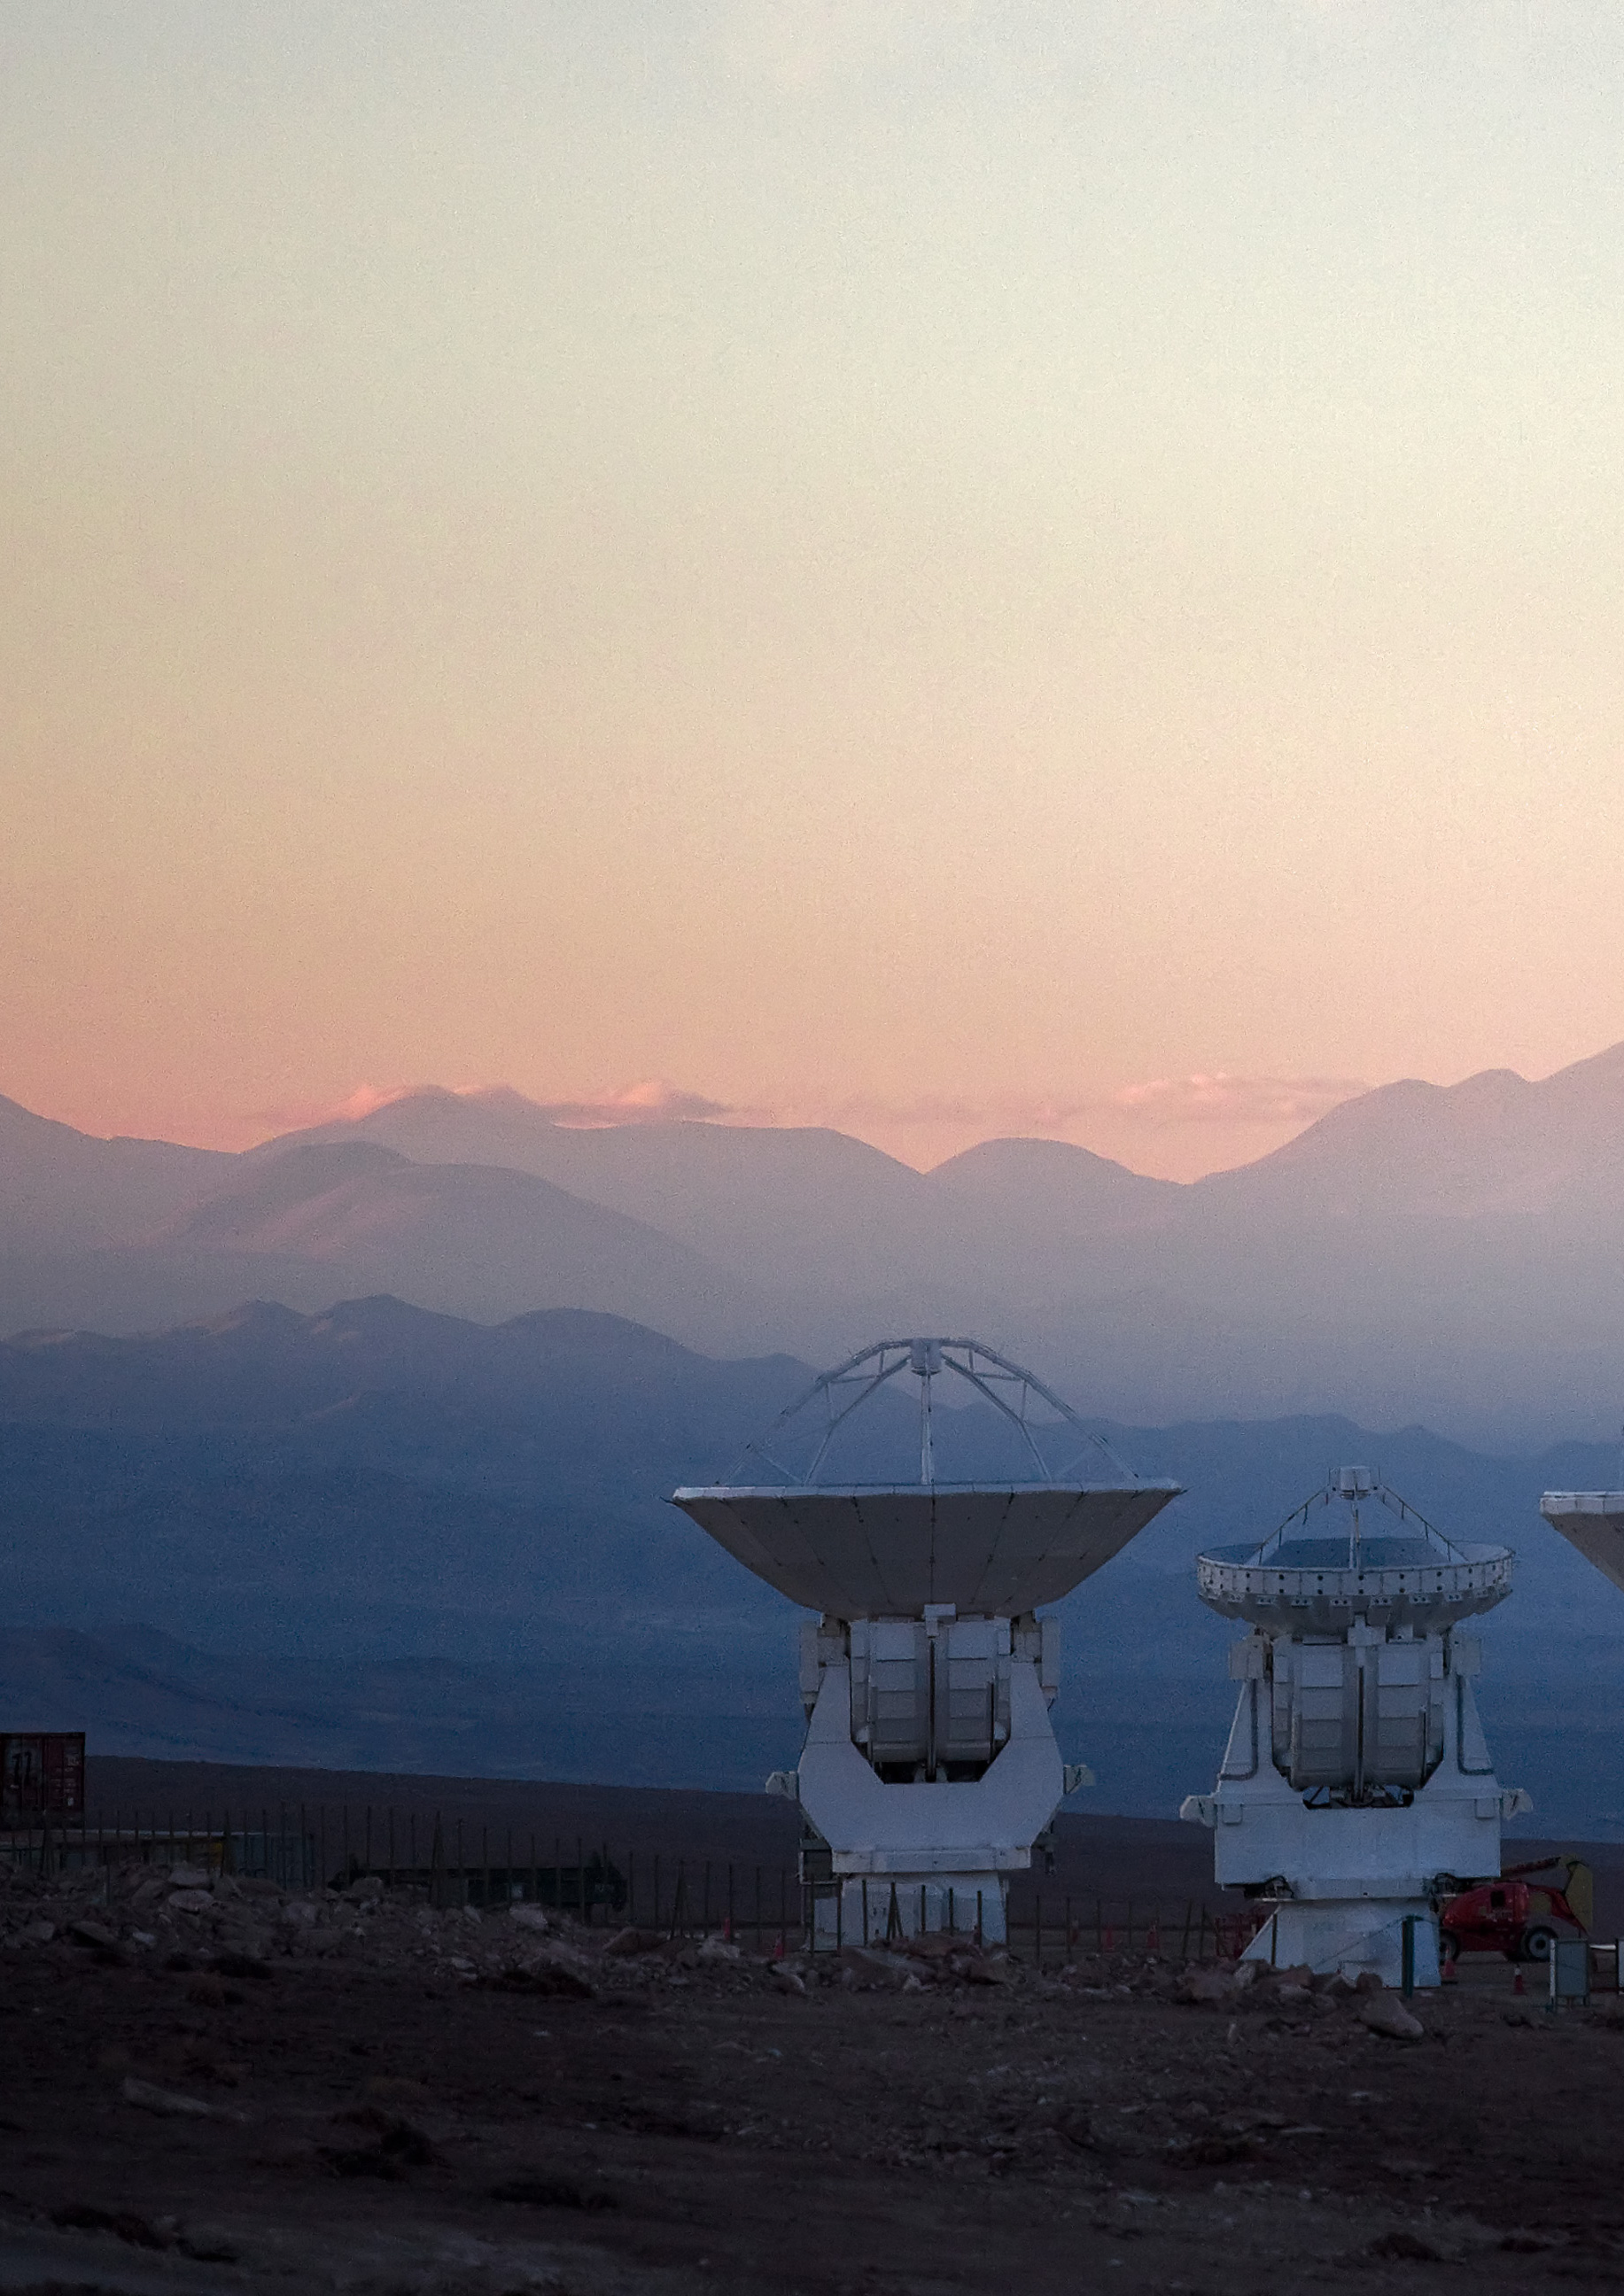
\includegraphics[width=\paperwidth]{Images/ALMA_antennas1}}
    }
    \BgThispage
    
    \fancyfoot[C]{\color{ALMAsky}\thepage}
    \fancyfoot[L]{\vspace{3.5ex}\tiny\textcolor{ALMAsky}{Credit: Iztok Bon\v{c}ina,\\ALMA (ESO, NAOJ, NRAO)}}
    \clearpage
    \newpage
\fi

\chapter[Dual constraints with ALMA]{Dual constraints with ALMA \\[2ex]\large{New \texorpdfstring{\OIIILam}{[O III] 88 μm} and dust-continuum observations reveal\\[-1ex]the ISM conditions of luminous LBGs at \texorpdfstring{$z \sim 7$}{z ∼ 7}}}
\label{ch:Dual_constraints_with_ALMA}

\ifsetDraft
\else
%    \vspace{8ex}
%    \setlength{\epigraphwidth}{0.25\textwidth}
%    \epigraph{\textit{Pulvis et umbra sumus.}
%        \\
%        \vspace{2ex}
%        \textit{We are dust and shadow.}}{--- Horace, Odes IV}

    %    \epigraph{\textit{What is a friend? One soul dwelling in two bodies.}}{--- Aristotle}
%    \vspace*{\fill}
    
    \backgroundsetup{
        scale=1,
        color=black,
        opacity=1,
        placement=top,
        angle=0,
        contents={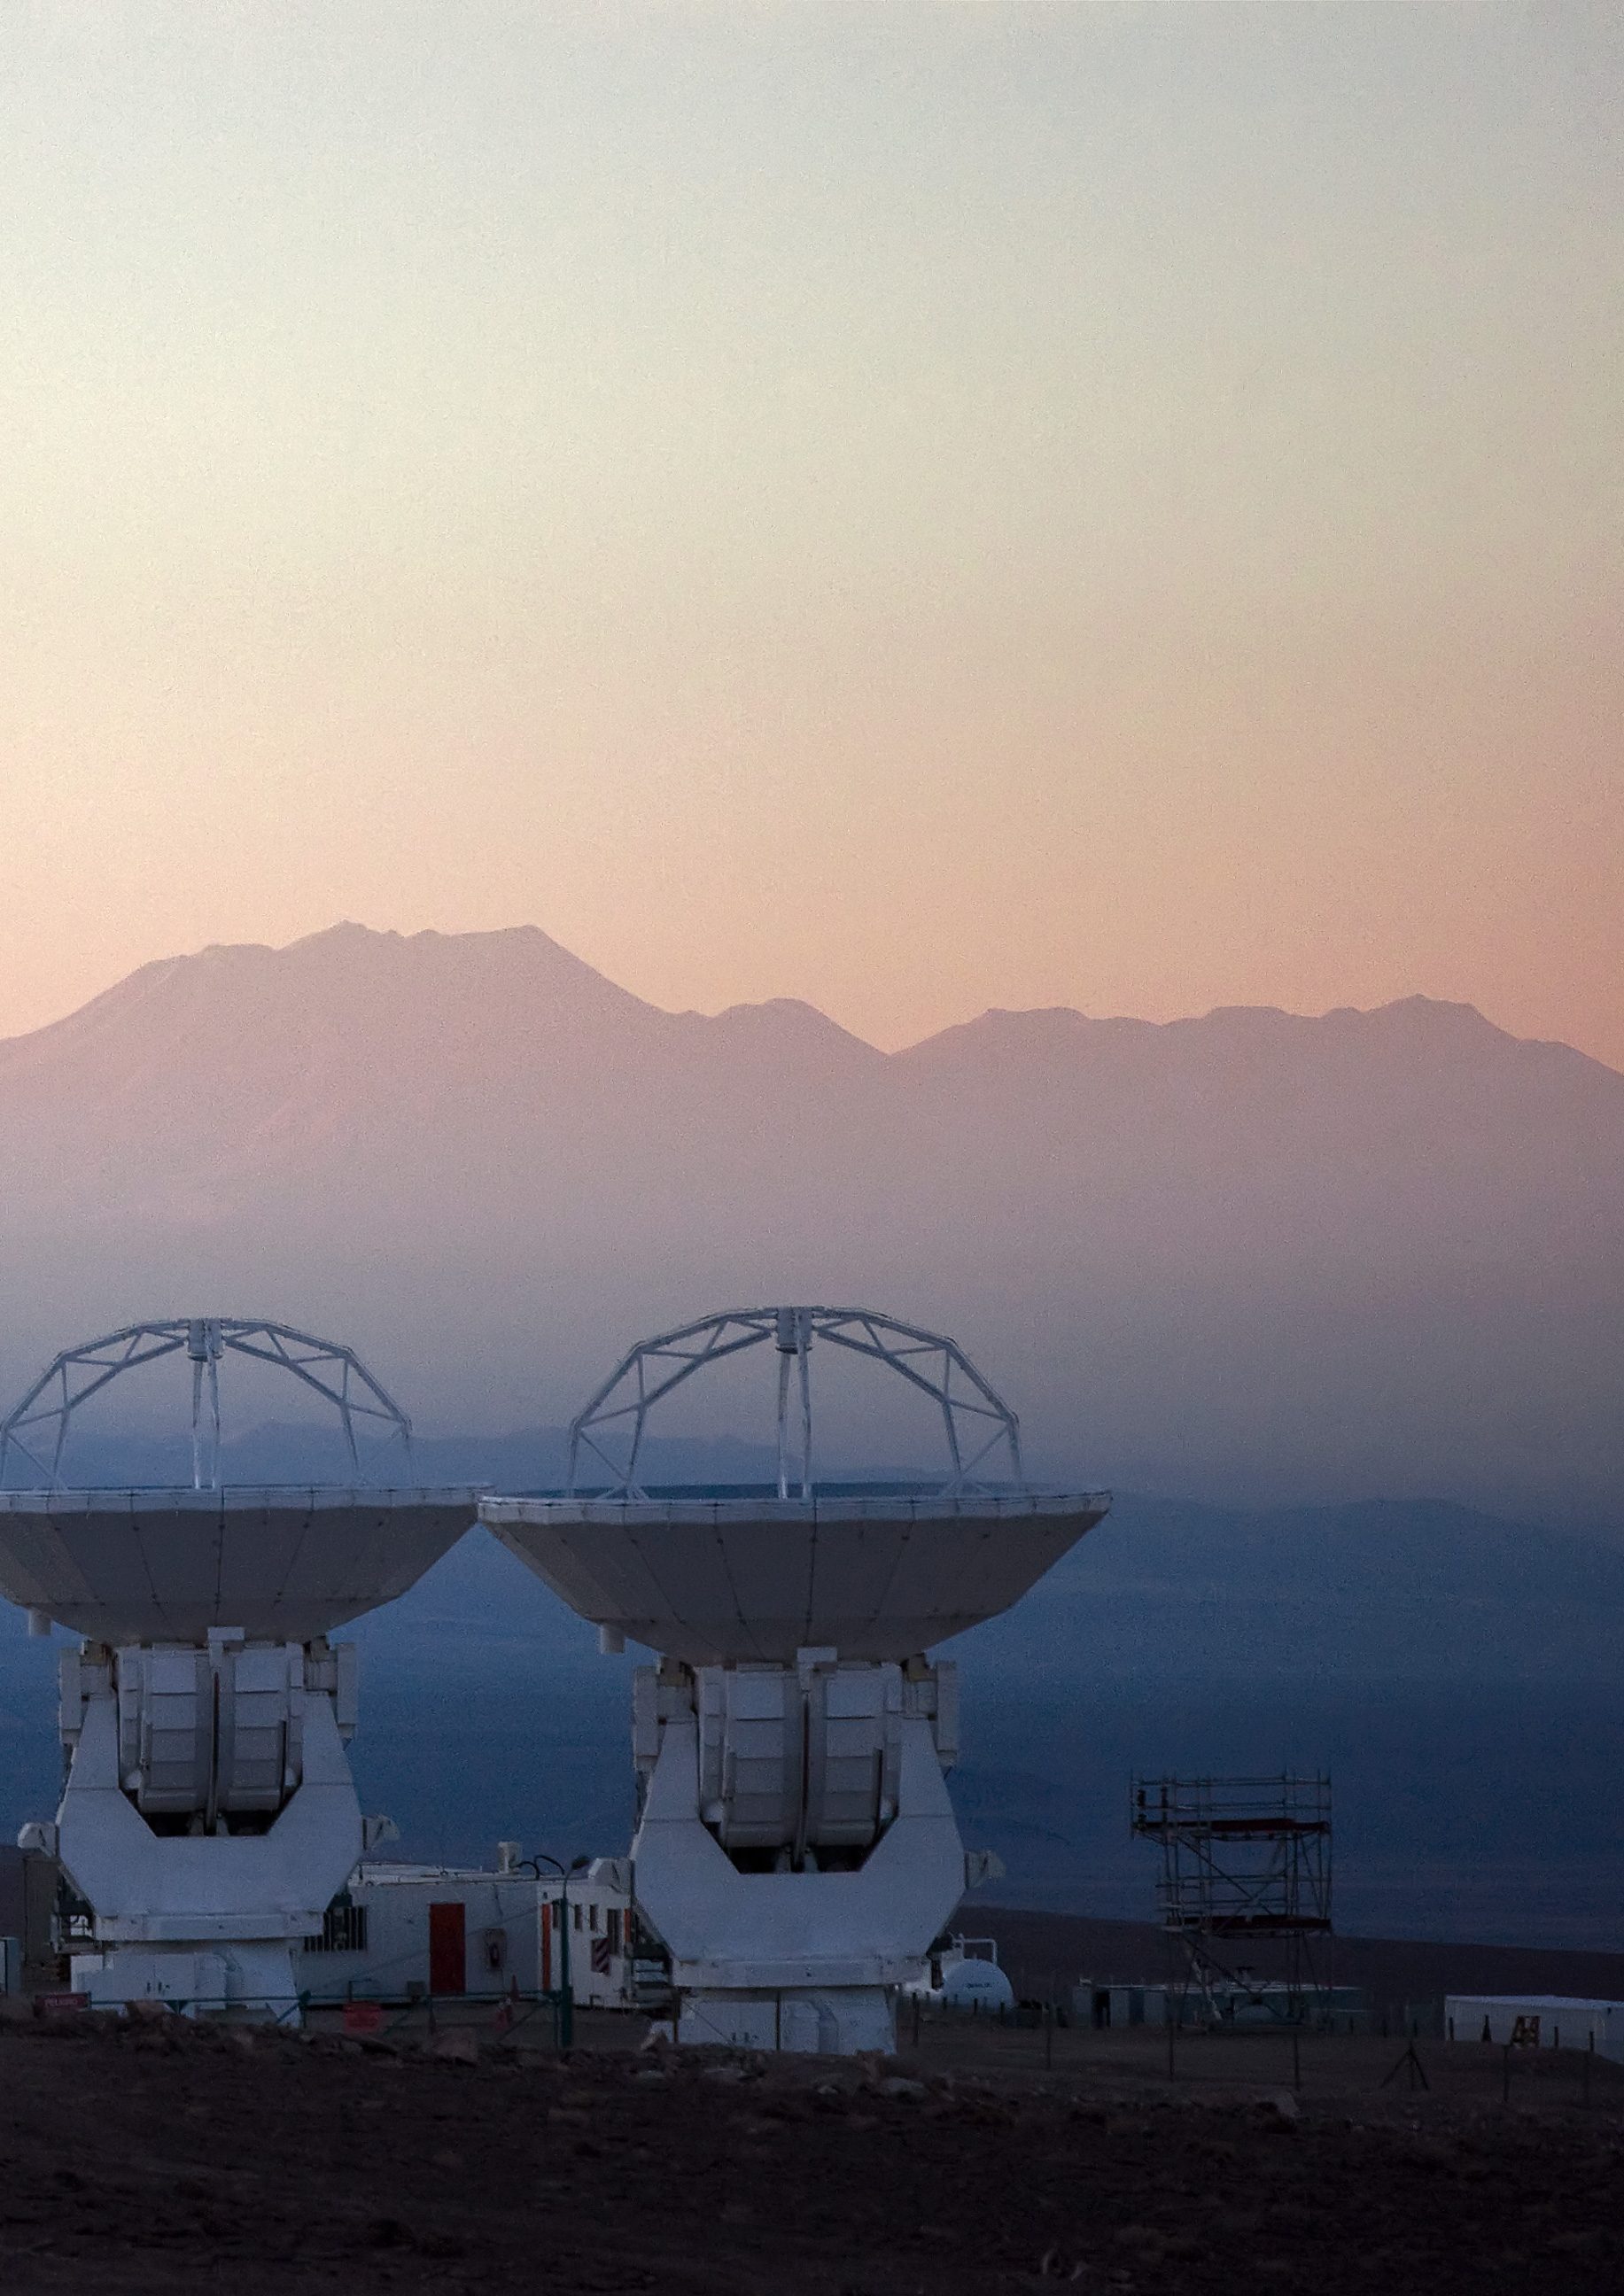
\includegraphics[width=\paperwidth]{Images/ALMA_antennas2}}
    }
    \BgThispage
    
    \fancyhf{}
    \fancyfoot[C]{\color{ALMAsky}\thepage}
    \newpage
    \setFancyHdr
\fi

\vspace*{\fill}

\noindent In this chapter, we present new \OIIILam\ observations of five bright $z \sim 7$ Lyman-break galaxies spectroscopically confirmed by ALMA through \CIILam, unlike recent \OIIIf\ detections where \lya\ was used. This nearly doubles the sample of Epoch of Reionisation galaxies with robust ($5 \sigma$) \CII\ and \OIIIf\ detections. We perform a multi-wavelength comparison with new deep \textit{HST} images of the rest-frame UV, whose compact morphology aligns well with \OIIIf\ tracing ionised gas. By contrast, we find more spatially extended \CII\ emission likely produced in neutral gas, as indicated by a \NIILam\ non-detection in one source. We find a correlation between the equivalent width of the optical \OIIIf\ and \Hbeta\ lines and \OIIIf/\CII, as seen in local metal-poor dwarf galaxies. \program{Cloudy} models of a nebula of typical density harbouring a young stellar population with a high ionisation parameter adequately reproduce the observed lines. Surprisingly, however, our models fail to reproduce the strength of \OIIILam, unless we assume an $\mathrm{\upalpha/Fe}$ enhancement and near-solar nebular oxygen abundance. On spatially resolved scales, we find \OIIIf/\CII\ shows a tentative anti-correlation with infrared excess, $L_\text{IR}/L_\text{UV}$, also seen on global scales in the local Universe. Finally, we introduce the far-infrared spectral energy distribution fitting code \program{mercurius} to show that dust-continuum measurements of one source appear to favour a low dust temperature and correspondingly high dust mass. This implies a high stellar metallicity yield and may point towards the need of dust production or grain-growth mechanisms beyond supernovae.

\vspace{3ex}
\begin{mdframed}[backgroundcolor=black!2.5]
    \textsl{This chapter is based on work carried out in collaboration with Renske Smit, Roberto Maiolino, Nimisha Kumari, Manuel Aravena, Leindert Boogaard, Rychard Bouwens, Stefano Carniani, Gareth C. Jones, Mauro Stefanon, Paul van der Werf, and Sander Schouws. It appeared in MNRAS as \citet{2022MNRAS.515.1751W}.}
\end{mdframed}
\vspace*{\fill}

\newpage

\section{Introduction}
\label{chDsec:Introduction}

\lettrine{T}{he epoch of reionisation} marks a critical turning point in the early Universe and its study is one of the frontiers in modern astrophysics. During the EoR, the first galaxies emerged and started to rapidly form stars, which in turn began to ionise the surrounding gas -- first the interstellar medium, and eventually the IGM \citep{2018PhR...780....1D, 2021arXiv211013160R}. Compared to their present-day counterparts, these galaxies have not had much time to build up an abundance of metals \citepalias[e.g.][]{2019A&ARv..27....3M}. This suggests they have metal-poor stellar populations, which results in an enhanced output of UV photons due to the hardened spectra of O- and B-type stars, in addition to containing a reduced amount of dust, implying these early galaxies generally experience less absorption of UV radiation \citep{2016ARA&A..54..761S}.

Regions where star formation takes place, especially in the very early Universe, therefore harbour stellar radiation fields with a strong intrinsic flux of ionising UV photons. Deep broadband surveys in the optical and IR by \textit{HST} have indeed proven an effective method of finding star-forming EoR galaxies via their rest-frame UV emission, having identified a considerable number through the Lyman-break technique \citep[currently nearly \num{2000} candidates at $z \geq 6$; see e.g.][]{2021AJ....162...47B}.

Even at the earliest stages of galaxy evolution, however, dust can be of major influence. Dust grains not only catalyse star formation through the formation of molecules \citep{2018MNRAS.474.1545C} and fragmentation of gas \citep{2006MNRAS.369.1437S}, but they also obscure our view of these UV-bright star-forming regions. Dust is able to absorb a significant proportion of stellar optical and UV light, re-emitting the absorbed energy as thermal IR radiation. It therefore poses observational challenges to the inference of SFRs solely from UV and optical measurements \citep{2012ARA&A..50..531K, 2014ARA&A..52..415M, 2020ApJ...902..112B}. Indeed, recent work renewed attention on an existing notion \citep{2020RSOS....700556H}: that a non-trivial fraction of high-redshift galaxies ($z \gtrsim 4$) may be so-called ``\textit{HST}-dark'' systems which, even in the deepest \textit{HST} imaging (reaching $H \sim 27 \, \mathrm{mag}$), appear completely obscured at observed optical and NIR wavelengths \citep{2018A&A...620A.152F, 2019ApJ...884..154W, 2019Natur.572..211W, 2021Natur.597..489F, 2021ApJ...923..215C, 2022ApJ...925...23M}. But while dust complicates the interpretation in the rest-frame UV and optical, its thermal emission also serves as a probe of the mass of the ISM \citep[e.g.][]{2017ApJ...837..150S}.

In recent years, the Atacama Large Millimeter/submillimeter Array (ALMA) has opened a new observational window for the study of star-forming galaxies at high redshift \citep[see][ for a review]{2020RSOS....700556H}. ALMA is uniquely positioned to observe their FIR emission at (sub)millimetre wavelengths, which serves a twofold purpose. First, these efforts allow ALMA to directly detect the dust continuum emission (\cref{chIssec:Observing_galaxies_across_cosmic_time}). The first explorations of the FIR SEDs of galaxies in the EoR with ALMA indicate that they may rapidly build up considerable amounts of dust \citep[e.g.][]{2015Natur.519..327W, 2017ApJ...837L..21L}. Second, nebular emission lines enable crucial spectroscopic redshift confirmations and offer valuable insights into ISM conditions by probing, for instance, the ionisation state, metal enrichment, and kinematics of the gas \citep[\cref{chIssec:Nebular_emission_and_emission-line_diagnostics}; see][ for a review]{2019ARA&A..57..511K}.

Nebular line emission typically arises in gas surrounding hot and massive stars (\cref{chIsssec:Photoionisation_by_stars}). Gas in close vicinity forms a photoionised \HII\ region populated by species with an ionisation potential higher than hydrogen (e.g. O$^{2+}$, which requires $\ssim 35 \, \mathrm{eV}$ to form), whereas shielded gas further out will contain low-ionisation species such as C$^+$ (the ionisation potential of neutral carbon, $11.3 \, \mathrm{eV}$, is just below that of hydrogen, $13.6 \, \mathrm{eV}$; \citealt{2005AAS...207.8117A}). These regions can transition into PDRs -- defined as mostly neutral gas where UV photons still play a significant role in the chemistry and/or heating -- in which carbon is partly photoionised \citep[instead of hydrogen, as in \HII\ regions;][]{1999RvMP...71..173H}. The variety of ionised and neutral gas reservoirs comprising the ISM can be traced by the many ISM coolants in the FIR, notably the \CIILam\ and \OIIILam\ fine-structure lines \citep[\CII\ and \OIIIf\ hereafter; see e.g.][]{2019PASJ...71...71H, 2019MNRAS.487.5902K, 2019MNRAS.487.1689P, 2020ApJ...896...93H, 2022ApJ...931..160B}. \OIIIf\ is almost exclusively produced in \HII\ regions, while \CII\ emission can arise in both \HII\ regions and PDRs. Other FIR emission lines further complement the picture: for instance, the \NIILam\ transition is a powerful proxy of the ionisation state of hydrogen in the \CII-producing ISM \citep[e.g.][]{2012A&A...542L..34N, 2014ApJ...782L..17D}.

The \CII\ and \OIIIf\ lines shift into high-frequency coverage of ALMA with sufficient atmospheric transmission (i.e. band 8) above redshifts $z \sim 2.8$ and $z \sim 5.8$, respectively (\cref{chIfig:Cloudy_spectra_redshift}). For galaxies in the EoR, where ground-based observing facilities are restricted to spectroscopic studies of weaker rest-frame UV lines such as the $\CIIIs \, \lambda \, 1907, \CIIIf \, \lambda \, 1909 \, \Angstrom$ doublet \citep[e.g.][]{2021ApJ...917L..36T}, observations of the \CII\ and \OIIIf\ with ALMA have first of all proven an effective spectroscopic confirmation tool, with almost as many UV-bright galaxies at $z > 6.5$ now having been spectroscopically confirmed via the \CII\ line as with \ion{H}{I} \lymana\ \citep[\lya;][]{2022ApJ...931..160B}. Moreover, the \OIIIf\ and \CII\ lines offer a powerful way of exploring ISM properties at high redshift, even in ``normal'' star-forming galaxies (i.e. $\text{SFR} \lesssim 100 \, \mathrm{M_\odot \, yr^{-1}}$).\footnote{For example, \citet{2018Natur.553..178S} presented \CII\ detections of two $z \sim 7$ photometric galaxy candidates using a combined on-source time of less than an hour, while typical spectroscopic observations of rest-frame UV lines require multiple hours of integration time on a $10 \, \mathrm{m}$-class telescope.} Finally, owing to its interferometric nature, ALMA produces spatially resolved spectroscopic measurements, in contrast to unresolved slit spectroscopy, which additionally faces the undesirable effect of slit losses.

In local starburst galaxies, \CII\ is observed to be the dominant FIR line, while in metal-poor dwarfs \OIIIf\ takes over this role ($L_\OIIIf/L_\CII > 1$; e.g. \citealt{2020ApJ...896...93H}). Critically, a large filling factor of diffuse, ionised gas emitting \OIIILam\ means metal-poor systems have a more porous ISM through which ionising radiation could ``leak'' \citep{2015A&A...578A..53C}. The relative strengths of emission lines, in particular the \OIIIf\ and \CII\ lines, are thus a powerful indicator of the physical state of the ISM. Interestingly, recent observations of galaxies in the EoR have systematically revealed \OIIIf/\CII\ ratios similar to or even exceeding those in local metal-poor dwarf galaxies \citep[e.g.][]{2020MNRAS.499.5136C}.

In summary, specific properties of the ISM that can be derived from combined observations of line and continuum emission with ALMA include the dust mass and temperature, probed through its thermal emission \citep[e.g.][]{2020MNRAS.493.4294B, 2021MNRAS.508L..58B, 2022ApJ...928...31S}, as well as the temperature, density, ionisation \citep[e.g.][]{2019MNRAS.489....1F, 2019MNRAS.487.1689P, 2021MNRAS.505.5543V}, metal enrichment \citep[e.g.][]{2015ApJ...813...36V}, and gas kinematics \citep[e.g.][]{2021MNRAS.507.3540J}, all of which can be inferred from emission line strengths and spectral profiles. In turn, a robust understanding of the ISM conditions in typical EoR star-forming galaxies -- that is, both of their dust and gas content -- is crucial in constructing a complete physical picture of star formation in this earliest epoch and therefore also of the process of cosmic reionisation.

\begin{landscape}
    \begingroup
    \renewcommand{\arraystretch}{1.25} % Default value: 1
    \begin{table}
        \centering
        \caption[Sources studied in this chapter.]
        {Sources studied in this chapter (colours for reference). Coordinates are given as right ascension ($\alpha_\text{J2000}$), declination ($\delta_\text{J2000}$), and redshift ($z$). These are followed by general properties of the galaxies: the apparent magnitude ($m_\text{UV}$) and luminosity ($L_\text{UV}$) of the rest-frame UV, the stellar mass ($M_*$), and the EW of the optical \OIIIf\ and \Hbeta\ lines, $\text{EW} ( \OIIIf + \Hbeta )$, as presented in the works by \citet{2015ApJ...801..122S, 2018Natur.553..178S} and \citet{2022arXiv220204080S, 2022ApJ...928...31S}.}
        \label{chDtab:Targets}
        \begin{tabular}{llllllll}
            \hline
            Source & $\alpha_\text{J2000} \, (\mathrm{h})$ & $\delta_\text{J2000} \, (\mathrm{deg})$ & $z$ & $m_\text{UV} \, (\mathrm{mag})$ & $L_\text{UV} \, (10^{11} \, \mathrm{L_\odot})$ & $M_* \, (10^9 \, \mathrm{M_\odot})$ & $\text{EW} ( \OIIIf + \Hbeta ) \, (\Angstrom)$ \\
            \hline
            % \textit{COSMOS} & & & & & & & \\
            \csvreader[separator=pipe, late after line=\\, head to column names]{Tables/ChapterD/ALMA_COSMOS_targets.csv}{}{\object & \RA & \Dec & \z & \mUV & \LUV & \M & \EW}
            % \textit{UVISTA} & & & & & & & \\
            \csvreader[separator=pipe, late after line=\\, head to column names]{Tables/ChapterD/ALMA_UVISTA_targets.csv}{}{\object & \RA & \Dec & \z & \mUV & \LUV & \M & \EW}
            \hline
        \end{tabular}
    \end{table}
    \endgroup
\end{landscape}

The main aim of this chapter is to analyse ALMA observations of the \CIILam, \OIIILam, \NIILam, and underlying dust continuum emission for a sample of five luminous, star-forming LBGs at $z \sim 7$. Specifically, we present new observations of the \OIIILam\ line with ALMA in addition to new \textit{HST} imaging, which significantly increases the number of EoR sources detected in both \CII\ and \OIIIf\ \citep[currently $9$, while only $5$ have detections of at least $5 \sigma$ in both lines;][]{2020MNRAS.499.5136C}. Moreover, the sample considered in this chapter arguably has a weaker selection bias since, in contrast to the existing studies, all galaxies have previously been spectroscopically confirmed through \CII\ instead of \lya. Before reionisation is completed, the latter can namely only escape from galaxies occupying ionised bubbles, which are indicative of overdense regions \citep[e.g.][]{2022MNRAS.515.5790L}.

Our outline is as follows. \Cref{chDsec:Observations} discusses the available ALMA and \textit{HST} data and \cref{chDsec:Results} briefly discusses the results of these observations. In \cref{chDsec:Discussion:Dust_properties,chDsec:Discussion:Emission_line_properties}, we compare our findings concerning respectively the dust continuum and emission lines to other works in the literature and discuss our findings. \Cref{chDsec:Summary} provides a summary.

In our analysis, we adopt the cosmological parameters $\Omega_{\text{m}, \, 0} = 0.3$, $\Omega_{\Lambda, \, 0} = 0.7$, and $H_0 = 70 \, \mathrm{km \, s^{-1} \, Mpc^{-1}}$ throughout (implying an angular scale of $5.2 \, \mathrm{kpc/arcsec}$ at $z=7$). All magnitudes are in the AB system \citep{1983ApJ...266..713O}.

\section{Observations}
\label{chDsec:Observations}

\subsection{Target selection}
\label{chDssec:Observations:Target_selection}

Five galaxies at $z \sim 7$, all located in the $\ssim 2 \, \mathrm{deg^2}$ UltraVISTA field \citep[UVISTA;][]{2012A&A...544A.156M}, are considered in this chapter: COS-2987030247, COS-3018555981, UVISTA-Z-001, UVISTA-Z-007, and UVISTA-Z-019 (\cref{chDtab:Targets}). The first two, COS-2987030247 and COS-3018555981, are contained in the \textit{HST} CANDELS field \citep{2011ApJS..197...35G} and were spectroscopically confirmed with ALMA observations of \CIILam\ in Cycle 3 \citep[ALMA project code 2015.1.01111.S;][]{2018Natur.553..178S}. The two sources were selected for their large optical emission line EWs, which enables an accurate photometric redshift determination using \textit{Spitzer}/IRAC broadband photometry at $3.6 \, \upmu\mathrm{{m}}$ and $4.5 \, \upmu\mathrm{{m}}$ \citep[see][ for details]{2015ApJ...801..122S}. The EWs of the optical \OIIIf\ (notably at $4960 \, \Angstrom$ and $5008 \, \Angstrom$) and \Hbeta\ lines (hereafter simply $\text{EW} ( \OIIIf + \Hbeta )$), presented in \citet{2015ApJ...801..122S}, are $\text{EW} ( \OIIIf + \Hbeta ) > \num{1000} \, \Angstrom$, while the median EW at $z \sim 7$ is around $\num{1000} \, \Angstrom$ \citep[see e.g.][]{2021MNRAS.500.5229E}. All five sources are bright in the UV, with apparent magnitudes between $24$ and $25 \, \mathrm{mag}$, implying $L_\text{UV} \sim 2 L_\text{UV}^* (z \sim 7)$. SED fitting with a \citet{2003PASP..115..763C} IMF yields stellar masses between $1$ and $4$ times $10^9 \, \mathrm{M_\odot}$ \citep[; see \cref{chDtab:Targets}]{2018Natur.553..178S, 2022ApJ...928...31S}.

The precise photometric redshift allowed ALMA to perform efficient blind spectral scans to search for the \CII\ line without first requiring a spectroscopic confirmation through \lya. Its success encouraged a second programme in Cycle 6 \citep[2018.1.00085.S;][]{2022arXiv220204080S} that has successfully detected the \CII\ line in three out of six additional galaxies, selected from ground-based imaging in the wider COSMOS field. Among these are the latter three sources considered here (UVISTA-Z-001, UVISTA-Z-007, and UVISTA-Z-019), two of which in comparison have modest EWs \citep[presented in][]{2022arXiv220204080S}, $\text{EW} ( \OIIIf + \Hbeta ) \sim 600$-$700 \, \Angstrom$, more typical for UV-bright LBGs at $z\sim7$ \citep[e.g.][]{2021MNRAS.500.5229E}. For an in-depth description of ALMA target selection strategies and scanning efficacy of \CII\ we refer to \citet{2022ApJ...931..160B}, introducing the successor of these two pilot programmes, the Reionization Era Bright Emission Line Survey (REBELS). This ALMA Large Program has targeted \CII\ and \OIIIf\ in $40$ of the brightest UV-selected star-forming galaxy candidates at $z > 6.5$.

\begin{landscape}
    \begingroup
    \setlength{\tabcolsep}{5pt} % Default value: 6pt
    \renewcommand{\arraystretch}{1} % Default value: 1
    \begin{table}
        \centering
        \caption[Overview of ALMA observations of the two $z \sim 7$ galaxies in the CANDELS-COSMOS field.]
        {Overview of ALMA observations of the two $z \sim 7$ galaxies in the CANDELS-COSMOS field. For each emission line observed, the observed frequency ($\nu_\text{obs}$), total on-source integration time ($t_\text{int}$), and channel width ($\Delta \nu_\text{obs}$) are shown. The first indicated beam size, $A_\text{beam}$ (given as the FWHMs of the major and minor axes), is the one tuned to match the beam between \CII\ and \OIIIf\ as closely as possible, which is achieved by the listed weighting scheme of either natural or Briggs weighting, an (optional) $uv$ taper, and the robust parameter (for Briggs weighting; see also \cref{chDsssec:Observations:ALMA_data_reduction}). The second beam size indicated for a line is one using natural weighting without tapering. The root-mean-square (RMS) noise (per channel of the given width) in naturally weighted images is shown in the second to last column, in good agreement with the theoretically predicted sensitivity (in brackets) computed for use in the \program{tclean} task (\cref{chDsssec:Observations:ALMA_data_reduction}). The final column lists the ALMA project codes (\cref{chDsssec:Observations:ALMA_programmes}).}
        \label{chDtab:Observations1}
        \begin{tabular}{lllllp{2.95cm}p{2cm}p{3.75cm}}
            \hline
            Source & Emission line & $\nu_\text{obs}$ & $t_\text{int}$ & $\Delta \nu_\text{obs}$ & Weighting scheme: $A_\text{beam}$ & RMS (sensitivity) & ALMA project \\
            & & ($\mathrm{GHz}$) & ($\mathrm{h}$) & ($\mathrm{MHz}$) & & ($\mathrm{\upmu Jy/beam}$) & code(s) \\
            \hline
            \csvreader[separator=pipe, late after line=\\, head to column names]{Tables/ChapterD/ALMA_COSMOS_observations.csv}{}{\ifcsvstrcmp{\field}{COSMOS}{\csviffirstrow{}{& & & & & & & \\}}{} \object & \emline & \freq & \int & \chanwidth & \beamsize & $\RMS \, (\sens)$ & \codes}
            \hline
        \end{tabular}
    \end{table}
    \begin{table}
        \centering
        \caption[Overview of ALMA observations of the three $z \sim 7$ galaxies in the UVISTA field.]
        {As \cref{chDtab:Observations1}, but for the three $z \sim 7$ galaxies in the UVISTA field.}
        \label{chDtab:Observations2}
        \begin{tabular}{lllllp{2.95cm}p{2cm}p{3.75cm}}
            \hline
            Source & Emission line & $\nu_\text{obs}$ & $t_\text{int}$ & $\Delta \nu_\text{obs}$ & Weighting scheme: $A_\text{beam}$ & RMS (sensitivity) & ALMA project \\
            & & ($\mathrm{GHz}$) & ($\mathrm{h}$) & ($\mathrm{MHz}$) & & ($\mathrm{\upmu Jy/beam}$) & code(s) \\
            \hline
            \csvreader[separator=pipe, late after line=\\, head to column names]{Tables/ChapterD/ALMA_UVISTA_observations.csv}{}{\ifcsvstrcmp{\field}{UVISTA}{& & & & & & & \\}{} \object & \emline & \freq & \int & \chanwidth & \beamsize & $\RMS \, (\sens)$ & \codes}
            \hline
        \end{tabular}
    \end{table}
    \endgroup
\end{landscape}

\subsection{ALMA data}
\label{chDssec:Observations:ALMA}

An overview of the ALMA observations considered in this chapter is shown in \cref{chDtab:Observations1,chDtab:Observations2}. In the following sections, we will briefly describe the existing ALMA observations of the \CIILam\ line, and the data reduction process of new measurements of the \OIIILam\ and \NIILam\ lines and the underlying dust continuum.

\subsubsection{ALMA programmes used in this study}
\label{chDsssec:Observations:ALMA_programmes}

In this study, we consider three main follow-up programmes of the bright Lyman-break galaxies that were confirmed with \CII\ described in \cref{chDssec:Observations:Target_selection}. COS-2987030247 was observed in band 5, targeting the \NIILam\ line with programme 2018.1.01551.S in Cycle 6 (note that for COS-3018555981 \NIILam\ falls into the atmospheric feature at the centre of band 5 and could not be included in this programme). All five bright \CII\ emitting galaxies described in \cref{chDssec:Observations:Target_selection}, were approved for A-ranked observations in band 8 in Cycle 6 (project code 2018.1.00429.S) and 7 (2019.1.01524.S) for the CANDELS-COSMOS and UVISTA sources, respectively.

Finally, we also make use of additional \CII\ data that was taken at high angular resolution ($\theta_\text{beam} < 0.2 \arcsec$), co-adding these with the low-resolution data for all sources except UVISTA-Z-007 (2017.1.00604.S, 2018.1.01359.S, 2019.1.01611.S). Similarly, we include additional band-6 observations of the dust continuum in UVISTA-Z-001 (2015.1.00540.S, 2018.1.00933.S) presented in \citet{2018MNRAS.481.1631B, 2022MNRAS.510.5088B}.

\subsubsection{ALMA data reduction}
\label{chDsssec:Observations:ALMA_data_reduction}

All data, including previous observations discussed above (see \cref{chDtab:Observations1,chDtab:Observations2}), were calibrated and reduced with the automated pipeline of the Common Astronomy Software Application \citep[\program{casa};][]{2007ASPC..376..127M} version 5.6 (with the exception of 2015.1.00540.S and 2015.1.01111.S, which required version 4.7).

Before the imaging step, we performed the \program{uvcontsub} task to separate the continuum and line visibilities specifically for imaging the \CII\ emission in COS-3018555981, UVISTA-Z-001, and UVISTA-Z-019 as well as the \OIIIf\ emission in UVISTA-Z-001, where the underlying dust continuum is confidently detected \citep[\cref{chDssec:Results:Dust_continuum}; see also][]{2022ApJ...928...31S}. Images were made with the \program{tclean} task for a large range of parameter sets, using all available data sets combined. We created images using both natural and Briggs weightings; under the natural weighting scheme, several different $uv$ tapers were considered as well as no taper. For measuring the total \OIIIf\ and \CII\ line fluxes, a moderately ($0.6 \arcsec$) tapered image was chosen to avoid resolving out extended emission \citep[see e.g.][]{2018MNRAS.478.1170C, 2020MNRAS.499.5136C} as best as possible while maintaining a good SNR. However, a natural weighting without any tapering was considered for the \NII\ line to maximise the SNR. Continuum images were created by averaging (i.e. the \program{mfs} mode in \program{tclean}) over all available spectral channels that were well outside the relevant emission line range (i.e. $\abs{v} > \num{1000} \, \mathrm{km/s}$). Natural weighting was again used for optimal SNR, however given the heterogeneity of the ALMA data, the following tapers were applied on a case-by-case basis to match the beams across various bands: $0.4 \arcsec$ for the band-6 data of COS-2987030247, $0.6 \arcsec$ for the band-6 data of COS-3018555981, $0.8 \arcsec$ for the band-8 data of UVISTA-Z-001, $1.0 \arcsec$ for the band-8 data of UVISTA-Z-007, and $0.2 \arcsec$ for the band-6 data of UVISTA-Z-019.

Finally, when comparing the \CII\ and \OIIIf\ lines, we also tuned the weighting or taper scheme to match the beam sizes as closely as possible. We use Briggs weighting for the line observed with lowest spatial resolution with a robust parameter tuned to the highest resolution achievable while maintaining a reasonable SNR. The other line is imaged with natural weighting and, if required, a small taper. \Cref{chDtab:Observations1,chDtab:Observations2} lists the resulting matched beam sizes for \CII\ and \OIIIf\ (as well as beam sizes obtained with an untapered, natural-weighting scheme). Furthermore, the measured root-mean-square (RMS) noise in naturally weighted images is compared in \cref{chDtab:Observations1,chDtab:Observations2} to the theoretically expected value of the sensitivity of an interferometric image \citep{2017isra.book.....T},\footnote{We note this is a simplified formula which leaves out a few additional system efficiencies; see Section 9.2.1 of the ALMA Technical Handbook \citep{ALMA_technical_handbook} for a more detailed form.}
\begin{equation}
    \label{chDeq:Interferometry_sensitivity}
    \delta S_\nu = \frac{2 k_\text{B} T_\text{sys}}{A_\text{eff} \sqrt{N_\text{ant} (N_\text{ant} - 1) t_\text{int} \Delta \nu}} \, ,
\end{equation}

\noindent where $k_\text{B}$ is the Boltzmann constant, $N_\text{ant}$ is the number of antennas (where we take the mean if observations obtained with multiple configurations are combined), $t_\text{int}$ is the total on-source integration time, $\Delta \nu$ is the channel width, $T_\text{sys}$ is the system temperature, and $A_\text{eff}$ is the effective collective area of each dish. Given the dish radius $r_\text{ant}$,
\begin{equation*}
    A_\text{eff} = \eta \pi r_\text{ant}^2 \, ,
\end{equation*}

\noindent which is equal to $\ssim 80 \, \mathrm{m^2}$ for the $12$-meter ALMA antennae assuming an efficiency factor of $\eta \sim 0.7$ \citep{ALMA_technical_handbook}. These sensitivities, which agree well with the empirically measured RMS noise, were computed for use in the \program{tclean} task, where the threshold parameter was set to three times this value.
\begin{figure}
    \centering
    \includegraphics[width=\linewidth]{"Plots/ChapterD/Dust_maps_clean_COS-3018555981_UVISTA-Z-001_UVISTA-Z-019"}
    \caption[Naturally weighted dust continuum maps of COS-3018555981, UVISTA-Z-001, and UVISTA-Z-019.]{Naturally weighted dust continuum maps of COS-3018555981 (first column), UVISTA-Z-001 (second column), and UVISTA-Z-019 (third column); beam sizes are indicated in the bottom left. Top row: clear detections at $\lambda_\text{emit} \sim 160 \, \mathrm{\upmu m}$ (imaged with varying degrees of taper; see \cref{chDsssec:Observations:ALMA_data_reduction,chDssec:Results:Dust_continuum}). Grey contours show subsequent significance levels in steps of $2 \sigma$ (COS-3018555981) or $1 \sigma$ (UVISTA-Z-001 and UVISTA-Z-019), starting at $3 \sigma$. White ellipses show the two-dimensional Gaussian fit obtained by \program{imfit} procedure in \program{casa}. Bottom row: (non-)detections at $\lambda_\text{emit} \sim 90 \, \mathrm{\upmu m}$. Contours are the same as the top row for UVISTA-Z-001, otherwise solid (dashed) grey lines show positive (negative) $1 \sigma$, $2 \sigma$, and $3 \sigma$ contours and white ellipses show the aperture used for determining a flux density upper limit (\cref{chDssec:Results:Dust_continuum}). Since there is significant extended emission at $\ssim 160 \, \mathrm{\upmu m}$ in UVISTA-Z-001, the white ellipses show the aperture used to measure the flux of the compact component in both the top and bottom panels (\cref{chDssec:Results:Dust_continuum}).
    }
    \label{chDfig:Dust_continuum_maps}
\end{figure}

\subsection{\textit{HST} imaging}
\label{chDssec:Observations:HST}

For sources at a redshift of $z \sim 7$, the rest-frame UV is observed in the NIR, ideally suited for observations with the infrared channel of the Wide Field Camera 3 (WFC3) on board \textit{HST}. For the two sources in the COSMOS field, COS-2987030247 and COS-3018555981, \textit{HST} imaging is available in the F125W ($J_{125}$), F140W ($JH_{140}$), and F160W ($H_{160}$) filters as part of CANDELS (GO 12440, PI: Faber) and the 3D-HST Treasury Programs (GO 12328, PI: Van Dokkum).\footnote{High-level science products are available on \url{https://archive.stsci.edu/prepds/3d-hst/}.} Combined, these observations reach a median depth of $26.1 \, \mathrm{mag}$, $25.5 \, \mathrm{mag}$, and $25.8 \, \mathrm{mag}$ ($5\sigma$ for a $1 \arcsec$-diameter aperture) in the $J_{125}$, $JH_{140}$, and $H_{160}$ bands, respectively \citep{2011ApJS..197...35G, 2011ApJS..197...36K, 2014ApJS..214...24S}. Throughout this chapter, we use a single stacked image, created by weighting the three filters by their inverse variance (covering $1400 \, \Angstrom \lesssim \lambda_\text{emit} \lesssim 2200 \, \Angstrom$). For UVISTA-Z-001, we use \textit{HST} imaging in the F140W filter (GO 13793, PI: Bowler) presented in \citet{2017MNRAS.466.3612B}.\footnote{Data may be obtained from the MAST at \href{https://dx.doi.org/10.17909/6gya-3b10}{10.17909/6gya-3b10}.}

For COS-2987030247, we manually remove a foreground source to the north-west. The foreground source is offset by just under $1 \arcsec$ and clearly (above $5 \sigma$) detected in the Advanced Camera for Surveys (ACS) F606W and F814W filters, while for sources at $z \sim 6.8$, the IGM would absorb any emission below the Lyman-continuum limit at a rest-frame wavelength of $912 \, \Angstrom$ (observed at $\ssim 0.7 \, \mathrm{\upmu m}$). In our stacked image, we replaced pixels with artificial noise if they are detected above $4 \sigma$ in a weighted ACS image that has been smoothed to match the slightly more extended PSF of WFC3.

In addition, \textit{HST} observations to acquire rest-frame UV imaging of UVISTA-Z-007 and UVISTA-Z-019 were awarded in Cycle 28 in the Mid-Cycle General Observer programme ID 16506 (PI: Witstok).\footnote{Data may be obtained from the MAST at \href{https://dx.doi.org/10.17909/t9-jhsf-m392}{10.17909/T9-JHSF-M392}.} Observations were performed with WFC3 using the F140W ($JH_{140}$) filter with a $5 \, \mathrm{ks}$ exposure per target, motivated by the goal of properly resolving the spatial substructure of the rest-frame UV. We divided each orbit into 4 exposures, which allows for a four-point dithering pattern to improve sampling of the PSF and to remove bad pixels, cosmic ray impacts, and detector artefacts. We used the \program{SPARS50} sampling sequence with $\program{nsamp}=13$ and $\program{nsamp}=14$ in two subsequent orbits for both targets.

Calibrated data products were combined using the \program{AstroDrizzle} task \citep[e.g.][]{2002PASP..114..144F} within the \program{DrizzlePac} package\footnote{See \url{https://www.stsci.edu/scientific-community/software/drizzlepac.html}.} setting the \program{final\_pixfrac} parameter to $0.8$ and choosing a pixel size of $0.065 \arcsec$. The resulting images reach a $5\sigma$ depth of $27.7 \, \mathrm{mag}$ for a $0.5 \arcsec$-diameter aperture (i.e. $25.9 \, \mathrm{mag/arcsec^2}$).

The astrometry of all images was calibrated to \textit{Gaia} data \citep{2016A&A...595A...1G, 2021A&A...649A...1G} by fitting a two-dimensional Gaussian to the \textit{HST} images of a number of nearby stars with a $g$-band magnitude of $g \lesssim 21 \, \mathrm{mag}$ ($7$, $5$, $6$, $4$, and $2$ for COS-2987030247, COS-3018555981, UVISTA-Z-001, UVISTA-Z-007, and UVISTA-Z-019, respectively). Among the stars in each field, we found the measured peak offsets relative to \textit{Gaia} positions agreed very well within less than $0.05 \arcsec$; taken together, they resulted in a required median correction of less than about $0.1 \arcsec$ in all cases.

\begingroup
\setlength{\tabcolsep}{6pt} % Default value: 6pt
\renewcommand{\arraystretch}{1.25} % Default value: 1
\newgeometry{left=14mm, right=14mm}
\begin{table}
    \centering
    \caption[Continuum fluxes]
    {Average, minimum, and maximum channel rest-frame wavelength and observed frequency used for the aggregate continuum images and corresponding (upper limits on) continuum fluxes. For non-detections, $3 \sigma$ upper limits are given (with theoretical $3 \sigma$ sensitivities, given by \cref{chDeq:Interferometry_sensitivity}, in brackets). For detections, deconvolved sizes $A_\text{dust}$ as measured by the \program{casa} \program{imfit} procedure are given. Dust-related quantities listed are the mass $M_\text{dust}$, mass surface density $\Sigma_\text{dust}$, and yield $y_\text{dust}$, discussed in \cref{chDssec:Discussion:Dust_masses}; the intrinsic SED temperature $T_\text{dust}$ and peak temperature $T_\text{peak}$, discussed in \cref{chDssec:Discussion:Dust_temperatures}; the integrated IR and FIR luminosities ($L_\text{(F)IR}$); and finally, the obscured and total SFRs, $\text{SFR}_\text{IR}$ and $\text{SFR}_\text{tot}$. These properties are inferred from \program{mercurius} fits where possible (i.e. for COS-3018555981, UVISTA-Z-001, and UVISTA-Z-019), under the fiducial self-consistent opacity model (for a more in-depth discussion, see \cref{chDssec:Discussion:Dust_SED_fitting_procedure}). Otherwise, they are approximated under a fully optically thin SED with the fiducial assumptions of $T_\text{dust} = 50 \, \mathrm{K}$, $\beta_\text{IR} = 1.5$, which however introduces large systematic uncertainties (see \cref{chDssec:Results:Dust_continuum} for details). For COS-3018555981, an upper limit ($95 \%$ confidence) on the dust temperatures is reported in brackets.}
    \label{chDtab:Continuum_fluxes_and_dust_properties}
    \footnotesize
    \begin{tabular}{llp{2.05cm}p{2.05cm}p{2.05cm}p{2.05cm}p{2.05cm}}
        \hline
        Regime & Quantity & \setulcolor{COS2987}\ul{COS-2987030247} & \setulcolor{COS3018}\ul{COS-3018555981} & \setulcolor{UVIS001}\ul{UVISTA-Z-001} & \setulcolor{UVIS007}\ul{UVISTA-Z-007} & \setulcolor{UVIS019}\ul{UVISTA-Z-019}
        \\
        \hline
        \multirow{4}{*}{Band 8} & $\nu_\text{obs} \, (\mathrm{GHz})$ & $426.2_{ -6.7 }^{ +9.3 }$ & $422.5_{ -5.4 }^{ +8.4 }$ & $413.0_{ -6.9 }^{ +8.9 }$ & $434.5_{ -7.7 }^{ +6.2 }$ & $434.4_{ -7.8 }^{ +6.1 }$
        \\
        & $\lambda_\text{{emit}} \, (\mathrm{{\upmu m}})$ & $90.1_{ -1.9 }^{ +1.4 }$ & $90.3_{ -1.8 }^{ +1.2 }$ & $90.0_{ -1.9 }^{ +1.5 }$ & $89.0_{ -1.3 }^{ +1.6 }$ & $89.0_{ -1.2 }^{ +1.6 }$
        \\
        & $S_{\nu, \, \text{obs}} \, (\mathrm{\upmu Jy})$ & $<163 \, (160)$ & $<210 \, (240)$ & $189 \pm 100$ & $<361 \, (260)$ & $<840 \, (625)$
        \\
        \vspace{1.5ex}
        & $A_\text{dust} \, (\mathrm{kpc^2})$ & \dots & \dots & $(5.2 \pm 2.4) \times$ \newline $(2.0 \pm 1.3)$ & \dots & \dots
        \\
        \multirow{4}{*}{Band 6} & $\nu_\text{obs} \, (\mathrm{GHz})$ & $250.3_{ -9.8 }^{ +7.3 }$ & $232.1_{ -8.0 }^{ +13.3 }$ & $232.9_{ -16.0 }^{ +10.0 }$ & $242.4_{ -2.1 }^{ +2.0 }$ & $237.3_{ -11.0 }^{ +8.8 }$
        \\
        & $\lambda_\text{{emit}} \, (\mathrm{{\upmu m}})$ & $153.4_{ -4.4 }^{ +6.2 }$ & $164.5_{ -8.9 }^{ +5.9 }$ & $159.6_{ -6.6 }^{ +11.8 }$ & $159.6_{ -1.3 }^{ +1.4 }$ & $162.9_{ -5.8 }^{ +7.9 }$
        \\
        & $S_{\nu, \, \text{obs}} \, (\mathrm{\upmu Jy})$ & $<22.5 \, (18.4)$ & $76 \pm 13$ & $97 \pm 30$ & $<69.6 \, (81.8)$ & $131 \pm 36$
        \\
        \vspace{1.5ex}
        & $A_\text{dust} \, (\mathrm{kpc^2})$ & \dots & $(4.3 \pm 0.8) \times$ \newline $(3.6 \pm 0.7)$ & $(10.3 \pm 3.4) \times$ \newline $(3.7 \pm 3.0)$ & \dots & $(4.1 \pm 1.1) \times$ \newline $(3.0 \pm 0.9)$
        \\
        \multirow{3}{*}{Band 5} & $\nu_\text{obs} \, (\mathrm{GHz})$ & $195.6_{ -9.4 }^{ +6.4 }$ & \dots & \dots & \dots & \dots
        \\
        & $\lambda_\text{{emit}} \, (\mathrm{{\upmu m}})$ & $196.3_{ -6.3 }^{ +9.9 }$ & \dots & \dots & \dots & \dots
        \\
        & $S_{\nu, \, \text{obs}} \, (\mathrm{\upmu Jy})$ & $<19.4 \, (22.8)$ & \dots & \dots & \dots & \dots
        \vspace{1ex}
        \\
%        &  &  &  &  &  & 
%        \\
        \cline{2-7}
        & $T_\text{dust}$ & Fixed: $50 \, \mathrm{K}$ & \program{mercurius} fit & \program{mercurius} fit & Fixed: $50 \, \mathrm{K}$ & \program{mercurius} fit
        \\
        & $\lambda_0$ (opacity) & Optically thin & Self-consistent: $8.4_{ -4.4 }^{ +11.8 } \, \mathrm{ \upmu m }$ & Self-consistent: $0.6_{ -0.3 }^{ +0.7 } \, \mathrm{ \upmu m }$ & Optically thin & Self-consistent: $4.2_{ -2.7 }^{ +7.5 } \, \mathrm{ \upmu m }$
        \\
        & $\beta_\text{IR}$ & Fixed: $1.5$ & Fixed: $1.5$ & Fixed: $1.5$ & Fixed: $1.5$ & Fixed: $1.5$
        \\
        \cline{2-7}
        \vspace{1ex}
%        &  &  &  &  &  & 
%        \\
        & $M_\text{dust} \, (\mathrm{M_\odot})$ & $\lesssim4 \cdot 10^{6}$ & $7_{-5}^{+19} \cdot 10^{7}$ & $4_{-3}^{+8} \cdot 10^{6}$ & $\lesssim1 \cdot 10^{7}$ & $2.1_{-1.6}^{+7.6} \cdot 10^{7}$
        \\
        & $\Sigma_\text{dust} \, (\mathrm{M_\odot \, pc^{-2}})$ & \dots & $7_{-4}^{+18}$ & $0.1_{-0.1}^{+0.3}$ & \dots & $2.3_{-1.8}^{+8.5}$
        \\
        & $M_\text{dust} / M_*$ & $\lesssim0.002$ & $0.05_{-0.04}^{+0.16}$ & $0.001_{-0.0007}^{+0.003}$ & $\lesssim0.003$ & $0.007_{-0.006}^{+0.03}$
        \\
        & $y_\text{dust, AGB} \, (\mathrm{M_\odot})$ & $\lesssim0.1$ & $1.5_{-1.1}^{+4.6}$ & $0.03_{-0.02}^{+0.08}$ & $\lesssim0.1$ & $0.2_{-0.2}^{+0.9}$
        \\
        \vspace{1.5ex}
        & $y_\text{dust, SN} \, (\mathrm{M_\odot})$ & $\lesssim0.2$ & $4.5_{-3.1}^{+13.3}$ & $0.09_{-0.06}^{+0.2}$ & $\lesssim0.3$ & $0.6_{-0.5}^{+2}$
        \\
        & $T_\text{dust} \, (\mathrm{K})$ & \dots & $29_{-5}^{+9}$ ($<48$) & $59_{-20}^{+41}$ & \dots & $47_{-17}^{+40}$
        \\
        \vspace{1.5ex}
        & $T_\text{peak} \, (\mathrm{K})$ & \dots & $26_{-5}^{+8}$ ($<43$) & $53_{-17}^{+37}$ & \dots & $42_{-15}^{+35}$
        \\
        $8$-$1000 \, \mathrm{\upmu m}$ & $L_\mathrm{IR} \, (\mathrm{L_\odot})$ & $\lesssim2.1 \cdot 10^{11}$ & $9.9_{-2.3}^{+6.8} \cdot 10^{10}$ & $2.0_{-1.3}^{+9.5} \cdot 10^{11}$ & $\lesssim6.9 \cdot 10^{11}$ & $3.1_{-1.8}^{+18.1} \cdot 10^{11}$
        \\
        \vspace{1.5ex}
        $42.5$-$122.5 \, \mathrm{\upmu m}$ & $L_\mathrm{FIR} \, (\mathrm{L_\odot})$ & $\lesssim1.4 \cdot 10^{11}$ & $6.4_{-1.6}^{+4.8} \cdot 10^{10}$ & $1.1_{-0.6}^{+1.1} \cdot 10^{11}$ & $\lesssim4.7 \cdot 10^{11}$ & $2.1_{-1.3}^{+4.2} \cdot 10^{11}$
        \\
        $\mathrm{IR}$ ($8$-$1000 \, \mathrm{\upmu m}$) & $\text{SFR}_\text{IR} \, (\mathrm{M_\odot \, yr^{-1}})$ & $\lesssim32$ & $15_{-3}^{+10}$ & $30_{-20}^{+142}$ & $\lesssim102$ & $46_{-27}^{+270}$
        \\
        $\mathrm{UV+IR}$ & $\text{SFR}_\text{tot} \, (\mathrm{M_\odot \, yr^{-1}})$ & $\lesssim54$ & $34_{-4}^{+10}$ & $79_{-20}^{+142}$ & $\lesssim128$ & $63_{-27}^{+270}$
        \\
        \hline
    \end{tabular}
\end{table}
\restoregeometry
\endgroup

\section{Results}
\label{chDsec:Results}

\subsection{Dust continuum}
\label{chDssec:Results:Dust_continuum}

Except for a $\ssim 4 \sigma$ detection in UVISTA-Z-001, the dust continuum at a rest-frame wavelength of $\lambda_\text{emit} \sim 90 \, \mathrm{\upmu m}$ remains undetected for the other sources. The same holds for the dust continuum of COS-2987030247 around the \NII\ line at $205 \, \mathrm{\upmu m}$. The continuum at $\lambda_\text{emit} \sim 160 \, \mathrm{\upmu m}$, however, is detected in COS-3018555981, UVISTA-Z-001, and UVISTA-Z-019 \citep[see also][]{2022ApJ...928...31S, 2022MNRAS.510.5088B}. Dust continuum maps of these sources are shown in \cref{chDfig:Dust_continuum_maps}.

For consistency in the flux measurements across different ALMA bands, their beams are matched by applying a slight taper to higher resolution data (see \cref{chDsssec:Observations:ALMA_data_reduction}). For COS-3018555981 and UVISTA-Z-019, we place $3 \sigma$ upper limits at $\ssim 90 \, \mathrm{\upmu m}$ by empirically measuring the RMS noise in a beam-shaped aperture matched in (convolved) size to the source extent at $\ssim 160 \, \mathrm{\upmu m}$; for COS-2987030247 and UVISTA-Z-007, a FWHM beam-sized aperture is used. Since there is significant extended emission at $\ssim 160 \, \mathrm{\upmu m}$ in UVISTA-Z-001, we measure fluxes of the compact component in an aperture centred on the peak of the emission and matched in (convolved) size to the source extent at $\ssim 90 \, \mathrm{\upmu m}$ (implications for the inferred dust properties will be discussed in \cref{chDsec:Discussion:Dust_properties}). In estimating the uncertainties on our continuum detections as well as upper limits, we conservatively take a systematic flux calibration uncertainty into account ($10 \%$ in band 5 and 6, $20 \%$ in band 8).\footnote{See Section A.9.2 of the ALMA Proposers' Guide \citep{ALMA_proposers_guide}.}

In \cref{chDtab:Continuum_fluxes_and_dust_properties}, all continuum measurements around the three emission lines (including $A_\text{dust}$, the deconvolved source extent in $\mathrm{kpc^2}$, if detected) are summarised. Also presented in \cref{chDtab:Continuum_fluxes_and_dust_properties} are other characteristics of the sources like their corresponding total IR and FIR luminosities (defined as the integrated luminosity between $8$ and $\num{1000} \, \mathrm{\upmu m}$ and between $42.5$ and $122.5 \, \mathrm{\upmu m}$ in the rest frame, respectively; see e.g. \citealt{2020ApJ...902...78R}) and other dust properties, leveraging constraints from the combined continuum measurements. These properties have been derived from a best-fit ``greybody'' spectrum \citep[e.g.][]{2014PhR...541...45C} if possible and will be discussed in more detail in \cref{chDsec:Discussion:Dust_properties}. When only upper limits are available (i.e. for COS-2987030247 and UVISTA-Z-007; see \cref{chDssec:Discussion:Dust_SED_fitting_procedure}), we report $3 \sigma$ upper limits on the IR and FIR luminosities by assuming a fiducial $\beta_\text{IR} = 1.5$ and $T_\text{dust} = 50 \, \mathrm{K}$; we acknowledge the uncertainty on these parameters by adding an additional $0.4 \, \mathrm{dex}$ systematic uncertainty to the integrated luminosities and corresponding obscured SFR \citep[cf.][]{2020MNRAS.499.5136C} before setting upper limits.

\subsection{\texorpdfstring{\NIILam}{[N II] 205 μm}}
\label{chDssec:Results:NII}

We placed a $3 \sigma$ upper limit on the \NII\ luminosity of COS-2987030247 by first measuring the RMS noise in the untapered, naturally-weighted datacube over a single beam (assuming the source is unresolved). We obtained an upper limit on the line flux in $\mathrm{Jy \, km/s}$ by scaling this noise to a range of channels covering twice the maximum FWHM between the \OIIIf\ and \CII\ lines (\cref{chDssec:Results:OIII_CII}), which we then converted to a luminosity, as shown in \cref{chDtab:Line_fluxes}. The lower limit on the \CIILam\ to \NIILam\ ratio is $L_\CII/L_\NII > 4.8$ ($3 \sigma$).
\begin{figure}
    \centering
    \includegraphics[width=\linewidth]{"Plots/ChapterD/Line_maps_spectra_clean_cube"}
    \caption[Detections of the \CII\ and \OIIIf\ lines.]{Detections of the \CIILam\ and \OIIILam\ lines. Top row: contour images of the \CII\ and \OIIIf\ lines overlaid on a background of \textit{HST} rest-frame UV images (see \cref{chDssec:Observations:HST}). The line images have matched beam sizes (as listed in \cref{chDtab:Observations1,chDtab:Observations2}) and are produced by collapsing all channels within the FWHM of the line (as those of the SNR determination, which however use natural weighting without tapering; \cref{chDssec:Results:OIII_CII}). Contours start at $3 \sigma$ and increase in steps of $5 \sigma$ for the \CII\ contours in COS-3018555981 and UVISTA-Z-019, $3 \sigma$ for the \OIIIf\ contours in COS-3018555981, $2 \sigma$ for both lines in UVISTA-Z-001, and $1 \sigma$ otherwise. Bottom row: SNR-weighted line spectra extracted from a $2 \sigma$ region in a naturally weighted image integrated over the FWHM (cf. \cref{chDssec:Results:OIII_CII}). Coloured channels, which were used to produce a subsequent moment-zero map for measuring the total line flux, indicate the line detection. The significance of each line detection is shown in the legend (also see \cref{chDssec:Results:OIII_CII} for details).
    }
    \label{chDfig:CII_and_OIII_maps_and_spectra}
\end{figure}

\begin{landscape}
    \begin{table}
        \centering
        \caption[Observed line fluxes of \CIILam, \OIIILam, and \NIILam.]
        {Observed line fluxes ($F_\text{line}$) of \CIILam, \OIIILam, and \NIILam, given in units of $\mathrm{Jy \, km/s}$ (i.e. as $S_\nu \Delta v$; see \cref{chDssec:Results:NII,chDssec:Results:OIII_CII} for details). Also shown are corresponding line luminosities and the \OIIIf/\CII\ luminosity ratio. For non-detections, $3 \sigma$ upper limits are given.}
        \label{chDtab:Line_fluxes}
        \begin{tabular}{llllllll}
            \hline
            Source & $F_\CII \, (\mathrm{Jy \, km/s})$ & $L_\CII \, (10^8 \, \mathrm{L_\odot})$ & $F_\OIIIf \, (\mathrm{Jy \, km/s})$ & $L_\OIIIf \, (10^8 \, \mathrm{L_\odot})$ & $L_\OIIIf/L_\CII$ & $F_\NII \, (\mathrm{Jy \, km/s})$ & $L_\NII \, (10^8 \, \mathrm{L_\odot})$ \\
            \hline
            \csvreader[separator=pipe, late after line=\\, head to column names]{Tables/ChapterD/ALMA_line_fluxes.csv}{}{\object & \SnudvCII & \LCII & \SnudvOIII & \LOIII & \OIIICII & \SnudvNII & \LNII}
            \hline
        \end{tabular}
    \end{table}
\end{landscape}

\subsection{\texorpdfstring{\OIIILam}{[O III] 88 μm} and \texorpdfstring{\CIILam}{[C II] 158 μm}}
\label{chDssec:Results:OIII_CII}

We obtained moment-zero maps by integrating a naturally weighted, clean datacube over the FWHM around the line centre. Defining the SNR as that measured for the peak pixel, the \OIIIf\ and \CII\ lines are detected with a significance of at least $\text{SNR} > 5$ in all five sources. Total line fluxes, however, are measured on cleaned cubes with a $0.6 \arcsec$ taper to recover extended emission as well as possible (\cref{chDsssec:Observations:ALMA_data_reduction}), integrating all channels where line flux is detected (coloured channels in \cref{chDfig:CII_and_OIII_maps_and_spectra}) in a spectrum extracted from a contiguous region of spaxels reaching at least $2 \sigma$ in the moment-zero map, the spectrum each spaxel weighted by its SNR. In turn, this initial moment-zero map was created by integrating channels within half of the FWHM from the line centre (used in the SNR determination described above). Again, we take a conservative systematic flux calibration uncertainty into account, as discussed in \cref{chDssec:Results:Dust_continuum}. The resulting line fluxes, luminosities, and ratios are listed in \cref{chDtab:Line_fluxes}.

\section{Dust properties}
\label{chDsec:Discussion:Dust_properties}

Although accounting for only a small fraction of baryonic matter in galaxies, dust is highly relevant in the context of galaxy evolution \citep[e.g.][]{2019MNRAS.489.1397L}. Representative dust properties of EoR galaxies, however, are still difficult to constrain with current observations partly due to the degeneracy between dust mass and temperature, complicated further by the dust opacity. Only in a few cases, multiple constraints on the FIR SED of normal star-forming galaxies ($\text{SFR} \lesssim 100 \, \mathrm{M_\odot \, yr^{-1}}$) in the EoR are available \citep[e.g.][]{2019PASJ...71...71H, 2020MNRAS.493.4294B, 2021MNRAS.508L..58B}. Here, we use the available band-6 detections in combination with the non-detections in band 8 to obtain further insights into the (F)IR luminosity, $L_\text{(F)IR}$, corresponding obscured and total SFR,\footnote{Obtained from the UV and IR luminosities using the conversions in \citet{2012ARA&A..50..531K}.} dust mass (\cref{chDssec:Discussion:Dust_masses}), and dust temperature (\cref{chDssec:Discussion:Dust_temperatures}) of typical UV-bright EoR galaxies.

\subsection{Dust SED fitting procedure}
\label{chDssec:Discussion:Dust_SED_fitting_procedure}

A dust-continuum detection at $\lambda_\text{emit} \sim 160 \, \mathrm{\upmu m}$ combined with a detection (UVISTA-Z-001) or even an upper limit (COS-3018555981 and UVISTA-Z-019) at $\lambda_\text{emit} \sim 90 \, \mathrm{\upmu m}$ can provide insight into the dust properties beyond those derived with a fixed temperature, emissivity, and opacity model. To investigate this in detail, we performed a fitting routine using the multimodal nested sampling algorithm \program{multinest} \citep[described in][]{2009MNRAS.398.1601F} implemented in \program{python} as the \program{pymultinest} package \citep{2014A&A...564A.125B}, as described below. The full code of this routine which treats detections and upper limits uniformly and we therefore refer to as \program{mercurius} (Multimodal Estimation Routine for the Cosmological Unravelling of Rest-frame Infrared Uniformised Spectra), is available online.\footnote{See \url{https://github.com/joriswitstok/mercurius/}.} Apart from the main fitting procedure, it also includes a greybody SED exploration visualisation tool; both are illustrated in a documented example.

The main properties of dust-continuum emission have been discussed in \cref{chIssec:Effects_of_dust}, but we repeat the main equations here. The flux density observed at $\nu_\text{obs} = \nu / (1+z)$, denoted $S_{\nu, \, \text{obs}}$ and given in $\mathrm{erg \, s^{-1} \, cm^{-2} \, Hz^{-1}}$, is given by the following general form of the observed SED \citep[\cref{chIeq:General_dust_SED_flux_density}, but see also][]{2020MNRAS.498.4109J},
\begin{equation}
    \label{chDeq:General_dust_SED_flux_density}
    S_{\nu, \, \text{obs}} = \frac{A_\text{dust} \left( 1+z \right)}{D_L^2 (z)} \left( 1 - e^{-\tau (\nu)} \right) \left[ B_\nu \left(T_\text{dust} \right) - B_\nu \left(T_\text{CMB} (z) \right) \right] \, .
\end{equation}

In our fiducial model, the optical depth is taken to be proportional to the dust mass surface density $\Sigma_\text{dust}$ via \cref{chIeq:Dust_mass_absorption_coefficient_definition},
\begin{equation}
    \label{chDeq:Dust_mass_absorption_coefficient_definition}
    \tau (\nu) \equiv \kappa_\nu \, \Sigma_\text{dust} = \kappa_\nu \, C \, \frac{M_\text{dust}}{A_\text{dust}} \text{, with } C \geq 1 \, ,
\end{equation}

\noindent where we take $A_\text{dust}$ to be the deconvolved size of the dust emission found by the \program{imfit} procedure in \program{casa} (given in \cref{chDtab:Continuum_fluxes_and_dust_properties}; see e.g. \cref{chDfig:Dust_continuum_maps}). Following \citet{2022ApJ...928...31S}, we used $\kappa_{\nu, \text{ ref}} = 8.94 \, \mathrm{cm^2 \, g^{-1}}$ at $\lambda_\text{ref} = 158 \, \mathrm{\upmu m}$ (i.e. $\nu_\text{ref} = \nu_\CII \simeq 1.90 \, \mathrm{THz}$), appropriate for dust ejected by SNe after reverse shock destruction (values for different dust grain compositions range from $5 \, \mathrm{cm^2 \, g^{-1}} \lesssim \kappa_{\nu, \text{ ref}} \lesssim 30 \, \mathrm{cm^2 \, g^{-1}}$; see \citealt{2014MNRAS.443.1704H}, and references therein). As will be discussed in \cref{chDssec:Discussion:Dust_masses}, SNe are the most likely origin of dust in these young, metal-poor star-forming galaxies. However, since the detailed dust composition is in principle unknown, $\kappa_{\nu, \text{ ref}}$ carries with it a systematic uncertainty that can lower dust masses by $\ssim 3 \times$ or increase them by $\ssim 1.5 \times$.

For Lyman-break galaxies at high redshift, the wavelength at which the dust transitions from optically thin to thick, $\lambda_0$, is typically assumed to be well below the sampled wavelength regime so that it is safe to approximate the entire SED as being optically thin \citep[$\tau (\nu) \ll 1$; e.g.][]{2021MNRAS.508L..58B} which simplifies \cref{chDeq:General_dust_SED_flux_density} (to the form in \cref{chIeq:OT_dust_SED_flux_density}). However, this assumption can lead to a significantly underestimated dust temperature and overestimated dust mass if incorrectly applied on measurements that sample a region where the approximation does not hold \citep{2020A&A...634L..14C, 2020MNRAS.498.4109J}.\footnote{Together with the fact that the intrinsic dust temperature has a large impact on the derived dust masses at shorter wavelengths, this is why dust masses should ideally be inferred from the highest FIR wavelengths ($\lambda_\text{emit} > 450 \, \mathrm{\upmu m}$), where the SED certainly is optically thin \citep{2012MNRAS.425.3094C}.} For a fixed $\lambda_0$, an a-posteriori consistency check on the assumed opacity model can be performed (see \cref{chIeq:Consistent_l0}),
\begin{equation}
    \label{chDeq:Consistent_l0}
    \lambda_0 = \left( \kappa_{\nu, \text{ ref}} \, \Sigma_\text{dust} \right)^{1/\beta_\text{IR}} \lambda_\text{ref} \, .
\end{equation}

Alternatively, \cref{chDeq:Consistent_l0} allows for a self-consistent framework around the general greybody SED model in \cref{chDeq:General_dust_SED_flux_density} where, given a dust mass, we infer $\lambda_0$ a priori, which we took as our fiducial opacity model.

Under a set opacity model, we then used a freely varying dust temperature and logarithmic dust mass. As the number of free parameters should not exceed the number of constraints and different assumptions of $\lambda_0$ typically dominate over those of the dust emissivity \citep{2014PhR...541...45C}, we -- conservatively, as will become clear in \cref{chDssec:Discussion:Dust_temperatures} -- fixed the dust emissivity to $\beta_\text{IR} = 1.5$. A flat prior within the range $10^4 \, \mathrm{M_\odot} < M_\text{dust} < M_*$ was assumed on $\log_{10} M_\text{dust}$; a gamma distribution with shape parameter $a = 1.5$ and shifted to start at $T_\text{CMB}(z)$ was used for the dust temperature (a standard choice for a parameter with a non-negative continuous domain as it is the conjugate prior to many likelihood distributions; we note that there is little difference when assuming a flat prior, but a maximum temperature has to be assumed). The model's predicted observed flux density at a given wavelength are compared with the actual observed flux densities and a likelihood is assigned based on the squared residuals between model and observations (weighted by the inverse variance). Following the formalism in \citet{2012PASP..124.1208S}, if the model greybody curve exceeds (falls below) the upper limits, the likelihood is lowered (increased) according to the significance of the discrepancy (agreement).

The full SEDs of four galaxies considered in this chapter are shown in \cref{chDfig:L_IR_constraints}. We show one of the two sources for which only upper limits on the dust continuum are available (COS-2987030247), where a range of dust temperatures ($30 \, \mathrm{K} \leq T_\text{dust} \leq 100 \, \mathrm{K}$) and emissivity parameters ($1.5 \leq \beta_\text{IR} \leq 2$) for templates that fit the constraints are considered instead of a \program{mercurius} fit (idem for UVISTA-Z-007 not shown here). These templates are created under an entirely optically thin opacity model (i.e. an SED described by \cref{chIeq:OT_dust_SED_flux_density}), which is a valid assumption since their dust masses are too small to be confidently detected (as shown in \cref{chDtab:Continuum_fluxes_and_dust_properties}). As can be seen from these templates, the constraints cannot be used to deduce the best-fit parameters, which is why we report (an upper limit on) the (F)IR luminosity and other parameters with a fiducial temperature $T_\text{dust} = 50 \, \mathrm{K}$ and $\beta_\text{IR} = 1.5$ (\cref{chDssec:Results:Dust_continuum}). From \cref{chDfig:L_IR_constraints}, it can furthermore be seen that the IR luminosity can vary by more than an order of magnitude between the most extreme choices of $T_\text{dust}$ and $\beta_\text{IR}$ \citep[see also][]{2020RSOS....700556H}. As described in \cref{chDssec:Results:Dust_continuum}, we take the systematic uncertainty resulting from fixing these parameters into account in our estimates of the (F)IR luminosity and obscured SFR.

For the three sources for which we have at least one $5 \sigma$ detection (COS-3018555981, UVISTA-Z-001, and UVISTA-Z-019), on the other hand, the \program{mercurius} fitting routine described above is applied, fixing $\beta_\text{IR} = 1.5$ but considering different assumptions on the opacity model: either an entirely optically thin SED or the general opacity model, with $\lambda_0$ set self-consistently or fixed to an extreme $200 \, \mathrm{\upmu m}$. The ``best-fit'' line shows the SED curve for the maximum likelihood in the $(M_\text{dust}, T_\text{dust})$ plane, shaded regions show the deviation of the \nth{16} and \nth{84} percentiles from the median (i.e. \nth{50} percentile) at each wavelength of all curves produced according to the posterior distribution. We note the best-fit model of COS-3018555981 and UVISTA-Z-019 is expected not to pass through the $\lambda_\text{emit} \sim 160 \, \mathrm{\upmu m}$ detection, since the upper limit at $\ssim 90 \, \mathrm{\upmu m}$ is also taken into account. In the next two sections, we will discuss the inferred dust properties in more detail.\footnote{Unless mentioned otherwise, reported quantities are given as the \nth{50} (i.e. median), \nth{16}, and \nth{84} percentiles (as a $\pm 1 \sigma$ confidence range) of the parameter's marginalised posterior distribution.}
\begin{figure}
    \centering
    \includegraphics[width=\linewidth]{"Plots/ChapterD/FIR_SED_constraints_COS-2987030247_COS-3018555981_UVISTA-Z-001_UVISTA-Z-019_beta_1.5"}
    \caption[Overview of the dust continuum detections and upper limits.]{Overview of the dust continuum detections and upper limits for four galaxies investigated in this chapter. Upper limits are drawn at $3 \sigma$, with a line beneath indicating a $1 \sigma$ level. Where only upper limits are available (i.e. for COS-2987030247), we plot a wide variety of greybody dust SEDs, for $30 \, \mathrm{K} \leq T_\text{dust} \leq 100 \, \mathrm{K}$ and $1.5 \leq \beta_\text{IR} \leq 2$ (under an entirely optically thin opacity model). The resulting range of IR luminosities is indicated in the bottom left, showing $L_\text{IR}$ can vary by more than an order of magnitude between the most extreme choices of $T_\text{dust}$ and $\beta_\text{IR}$. For COS-3018555981, UVISTA-Z-001, and UVISTA-Z-019, on the other hand, the \program{mercurius} fitting routine described in \cref{chDssec:Discussion:Dust_SED_fitting_procedure} is applied, fixing $\beta_\text{IR} = 1.5$ but considering various assumptions on the opacity model: either an entirely optically thin SED or the general opacity model given in \cref{chIeq:Optical_depth} with either a self-consistent or fixed $\lambda_0$, the wavelength separating the optically thick and thin regimes. The ``best-fit'' line shows the SED curve for the maximum likelihood in the $(M_\text{dust}, T_\text{dust})$ plane, shaded regions show the \nth{16} and \nth{84} percentiles at each wavelength of all curves produced according to the posterior distribution. We note the best-fit model of COS-3018555981 and UVISTA-Z-019 is expected not to pass through the $\lambda_\text{emit} \sim 160 \, \mathrm{\upmu m}$ detection, since the upper limit at $\ssim 90 \, \mathrm{\upmu m}$ is also taken into account. The resulting dust mass and temperature are indicated for each fit, as is $\lambda_0^\text{AP}$, the value of $\lambda_0$ that is inferred a posteriori (if applicable). The inferred peak temperature (though measured on the CMB-corrected spectrum; \cref{appDsec:Dust peak temperature measurements}) for the fiducial self-consistent opacity model is annotated (see also \cref{chDtab:Continuum_fluxes_and_dust_properties}).
    }
    \label{chDfig:L_IR_constraints}
\end{figure}

\subsection{The build-up of dust: masses and yields}
\label{chDssec:Discussion:Dust_masses}

First, we briefly discuss the estimates of the dust mass of our sources, while stressing these are fairly uncertain, firstly due to the range of possible $\kappa_\nu$ depending on the dust composition as discussed in \cref{chDssec:Discussion:Dust_SED_fitting_procedure}. Secondly, our measurements do not probe the Rayleigh-Jeans (RJ) tail of the SED, meaning that the dust mass becomes sensitive on the intrinsic dust temperature: sampling at a rest-frame wavelength $200 \, \mathrm{\upmu m}$ introduces a factor $\ssim 5$ difference in $M_\text{dust}$ for a $2 \times$ difference in $T_\text{dust}$, for instance \citep{2020A&A...634L..14C}. The latter effect, however, is reflected in the uncertainty estimates from the posterior distributions obtained in the \program{mercurius} fitting routine, which probes a range of temperatures. As will be discussed below, the distributions are based purely on the likelihood of underlying dust masses and temperatures producing the observed continuum (non-)detections and in principle could result in unphysical scenarios (save dust masses above the stellar mass and temperatures below the CMB temperature, whose solutions are discarded; \cref{chDssec:Discussion:Dust_SED_fitting_procedure}).

For the five sources considered in this chapter, we find the dust mass typically range upwards of a few million solar masses. Interestingly, the tentatively low dust temperature of COS-3018555981 (discussed in more detail in \cref{chDssec:Discussion:Dust_temperatures}) under the fiducial self-consistent general opacity model (where $\lambda_0 \simeq 10 \, \mathrm{\upmu m}$) nominally implies a relatively high dust mass, $M_\text{dust} = 7_{-5}^{+19} \cdot 10^7 \, \mathrm{M_\odot}$. Since the self-consistently derived $\lambda_0$ is well below the lowest sampled wavelength ($\lambda_\text{emit} \sim 90 \, \mathrm{\upmu m}$), an optically thin SED appears a rather good approximation producing a similar dust mass and temperature, although the estimated uncertainty in the self-consistent model is larger and thus more conservative (mainly allowing for even higher dust masses that are compensated for by an increasing $\lambda_0$).

The estimated dust mass translates into a substantial dust-to-stellar mass ratio, $M_\text{dust}/M_* = 0.05_{-0.04}^{+0.16}$ (\cref{chDtab:Continuum_fluxes_and_dust_properties}). Although we stress the current evidence is limited, the formal likelihood treatment evidently yields rather extreme solutions; might we expect the true values be more modest from a physical perspective? We consider dust grains comprise of metals mainly produced by short-lived, massive stars, while most of the stellar mass instead is dominated by low-mass stars, so that $M_\text{dust}/M_*$ cannot exceed the stellar metallicity yield -- the mass-fraction of metals released into the ISM compared to the total (remaining) stellar mass -- typically assumed to be a few percent \citepalias{2019A&ARv..27....3M}. However, higher stellar yields are certainly plausible for a (more) top-heavy IMF: for instance, a \citet{2001MNRAS.322..231K} or \citet{2003PASP..115..763C} IMF already results in stellar metallicity yields that are twice as high than for a \citet{1955ApJ...121..161S} IMF \citep{2016MNRAS.455.4183V}. Moreover, we note the stellar mass estimate of $M_* = 1.4_{-0.2}^{+0.7} \cdot 10^9 \, \mathrm{M_\odot}$ \citep[taken from][]{2018Natur.553..178S} is a conservative one in this context as it is $\ssim 0.5 \, \mathrm{dex}$ higher than the best fit found by the REBELS collaboration, who explored several photometric fitting codes \citetext{private communication, REBELS collaboration 2021; see also \citealt{2022ApJ...931..160B}}. Upcoming \textit{JWST} observations (GTO: 1217, GO: 1837) will provide a highly accurate stellar mass and give insight into the star formation history of this source, and hence also its age.

By assuming a stellar IMF, the dust-to-stellar mass ratio can be converted into a dust yield, denoted $y_\text{dust}$, which represents the average dust mass formed per dust-producing star. Here, we follow the method of \citet{2015A&A...577A..80M}, who considered SNe and AGB stars as sources of dust production, assuming their relevant stellar mass ranges are $8$-$40 \, \mathrm{M_\odot}$ and $3$-$8 \, \mathrm{M_\odot}$, respectively. Both yields from SNe and AGB stars for a \citet{2003PASP..115..763C} IMF are shown in \cref{chDtab:Continuum_fluxes_and_dust_properties}. Average AGB dust yields that are obtained under \citeauthor{1955ApJ...121..161S} and top-heavy IMFs can be $\ssim 2 \times$ higher, but this only strengthens the interpretation discussed below. More critically, however, the inferred SN dust yields could decrease (increase) by a factor of $\ssim 1.5$ for a top-heavy (\citeauthor{1955ApJ...121..161S}) IMF since these IMFs result in a higher (lower) number of SN events, thereby lowering (raising) the required average yield per SN.

The yield that would be required per AGB star, $y_\text{dust, AGB} \sim 1.5_{-1.1}^{+4.6} \, \mathrm{M_\odot}$ for COS-3018555981, far exceeds the theoretically expected value, $\ssim 0.02 \, \mathrm{M_\odot}$, even more so when the yield is increased up to $2 \times$ under a different IMF \citep[as already shown for other EoR galaxies in e.g.][]{2015A&A...577A..80M, 2019A&A...624L..13L, 2022ApJ...928...31S}. This renders AGB stars an unlikely candidate as the main source of dust formation in this early cosmic epoch (even within the systematic uncertainty of $\kappa_{\nu, \text{ ref}}$). Instead, when SNe are considered, a nominally gigantic yield of $y_\text{dust, SN} = 4.5_{-3.1}^{+13.3} \, \mathrm{M_\odot}$ per dust-producing star would be required. We note that the uncertainty estimates, apart from incorporating a systematic $10 \%$ flux calibration uncertainty (\cref{chDssec:Results:Dust_continuum}), are purely statistical and the SN dust yield could systematically be reduced by a high $\kappa_{\nu, \text{ ref}}$ resulting in a lower dust mass (see \cref{chDssec:Discussion:Dust_SED_fitting_procedure}). However, as also discussed in \cref{chDssec:Discussion:Dust_SED_fitting_procedure}, the current assumption of $\kappa_{\nu, \text{ ref}} = 8.94 \, \mathrm{cm^2 \, g^{-1}}$ is valid for dust produced by SNe and thus other choices would be inconsistent for estimating the SN dust yield.

Even the lowest required yield within the estimated $1 \sigma$ uncertainties, $\ssim 1.4 \, \mathrm{M_\odot}$, is already in slight tension with the maximum theoretical yield per SN, which is $1$ to $2 \, \mathrm{M_\odot}$ without the subsequent dust destruction by the SN \citep[e.g.][]{2003ApJ...598..785N}. The discrepancy might even be more serious for various reasons: if dust destruction does play a significant role, this lowers the theoretical maximum yield, while the required dust yield per SN is increased under a different IMF. Finally, we find yet a lower dust temperature and higher mass and yield increase if we instead assume a higher dust emissivity $1.8 \lesssim \beta_\text{IR} \lesssim 2$, the value typically found at high redshift for more massive systems \citep[e.g.][]{2020MNRAS.498.4109J, 2020A&A...634L..14C, 2020MNRAS.498.4192F, 2021ApJ...923..215C} -- this is why we conservatively opt for a fiducial $\beta_\text{IR} = 1.5$ here. Hence, there is tentative evidence that other evolutionary mechanisms, such as the growth of dust grains in the ISM \citep{2019A&A...624L..13L}, need to be invoked. A final caveat to this result is that the dust mass decreases if $\lambda_0$ is fixed to $200 \, \mathrm{\upmu m}$ (since higher temperatures are feasible in this scenario; \cref{chDssec:Discussion:Dust_temperatures}), thereby bringing the dust yield down to $y_\text{dust, SN} \sim 3 \, \mathrm{M_\odot}$, which however is still inconsistent with theoretical expectations. Yet this scenario would perhaps be equally surprising, as will be discussed further in \cref{chDssec:Discussion:Dust_temperatures}.
\begin{figure}
    \centering
    \includegraphics[width=0.8\linewidth]{"Plots/ChapterD/Redshift_T_peak"}
    \caption[Dust peak temperature as a function of redshift.]{Dust peak temperature, $T_\text{peak}$, as a function of cosmic time. Several peak temperatures derived from measurements presented in this chapter under the self-consistent general opacity model are drawn: for UVISTA-Z-019, we show its median and $68\%$ confidence range (largely invariant under the chosen opacity model), while for COS-3018555981 an upper limit ($95\%$ confidence) is shown in addition. Further, measurements inferred from stacked spectra and a (partially extrapolated) linear fit by \citet{2018A&A...609A..30S} are shown, as is the power-law fit to the peak-temperature evolution of simulated galaxies by \citet{2019MNRAS.489.1397L}. Details on the literature data points can be found in \cref{appDsec:Dust peak temperature measurements} (SMGs are shown as squares, other high-redshift galaxies as circles with errorbars). Three sources are highlighted with labels, having either a notably low (J0217-0208), high (MACS0416-Y1), or accurately constrained dust temperature (A1689-zD1). The grey dashed line shows the CMB temperature over cosmic time, the grey area below representing astrophysically unattainable temperatures -- we note, however, that effective peak temperatures of greybody SEDs can in principle fall below this boundary as they are lower than the dust temperature itself (\cref{chDssec:Discussion:Dust_temperatures}). The light-red area above indicates the region where CMB heating has a significant (greater than $1\%$) effect compared to $z=0$ (see \cref{chDssec:Discussion:Dust_temperatures} for details).
    }
    \label{chDfig:T_peak_evolution}
\end{figure}

\subsection{Cosmic evolution of dust temperature: evidence for extremely cold or highly clustered dust?}
\label{chDssec:Discussion:Dust_temperatures}

In the following, we move on to discuss the dust temperature, arguably one of its most important properties as it is essential in deriving other observable quantities such as the infrared luminosity and dust mass from a limited number of photometric data points \citep{2020MNRAS.497..956S, 2022MNRAS.513.3122S}. Unfortunately, establishing the dust temperature is not trivial. Directly fitting observed SEDs necessarily yields a luminosity-weighted dust temperature, which may be skewed towards high temperatures by hot dust in star-forming regions \citep{2019MNRAS.489.1397L}. Hot dust can only be observed directly, however, if the emission is optically thin \citep{2020MNRAS.498.4192F}. When little information is available, these effects cause the dust temperature, mass, and opacity to become degenerate.

In \cref{chDfig:T_peak_evolution}, measurements of the SED peak temperature across cosmic time are shown. The peak temperature is defined as a purely observational quantity, defined similarly to Wien's displacement law using the SED peak wavelength\footnote{The peak of the intrinsic SED, i.e. after it has been corrected for observing the dust emission against the CMB (\cref{chDssec:Discussion:Dust_SED_fitting_procedure}).} in the rest frame, $\lambda_\text{emit, peak}$:
\begin{equation}
    \label{chDeq:T_peak}
    T_\text{peak} = \frac{b}{\lambda_\text{emit, peak}} \text{, where } b \simeq 2898 \, \mathrm{K / \upmu m}.
\end{equation}

Details on the motivation for comparing peak temperatures, rather than $T_\text{dust}$, and the precise data from the literature that is included can be found in \cref{appDsec:Dust peak temperature measurements}. We report ``intrinsic'' peak temperatures, in the sense that there is no conversion to the current epoch ($z=0$) to nullify the effect of CMB heating at the relevant epoch, for two reasons. Firstly, peak temperatures are an observational construct (lower than the intrinsic dust temperature), and secondly, in most cases, the dust has already largely decoupled from the CMB and heating \citep[described by equation (12) of][]{2013ApJ...766...13D} starts to become relevant only when going back in cosmic time significantly or for extremely cold dust that has cooled down nearly to the CMB temperature. This is illustrated by the red shaded region, which marks an increase of more than $1\%$ in dust temperature between $z=0$ and the relevant redshift (under $\beta_\text{IR} = 1.5$) and falls below almost all measurements shown here (although neglected in \cref{chDfig:T_peak_evolution}, we will apply this correction when relevant in the following).

Although a consistent picture starts to emerge at $z \lesssim 4$ \citep[e.g.][]{2018A&A...609A..30S, 2022ApJ...930..142D}, it is unclear whether this also applies to galaxies in the EoR due to limited observational data and the highly uncertain relative importance of the possible mechanisms of dust formation \citep{2015MNRAS.451L..70M}. Theoretical models predict elevated dust temperatures compared to the local Universe \citep[e.g.][]{2019MNRAS.487.1844M, 2020MNRAS.497..956S, 2022MNRAS.511.4999V}, which is indeed confirmed by observations in some cases \citep[with extreme examples given in][]{2018MNRAS.477..552B, 2020MNRAS.493.4294B, 2022MNRAS.tmpL..72V}. However, the peak temperatures for several objects -- most notably $T_\text{peak} \sim 28 \, \mathrm{K}$ seen in J0217-0208 \citep{2020ApJ...896...93H} -- are lower than what may be expected from an extrapolation of the trend at low redshift (such as the shown fit by \citealt{2018A&A...609A..30S}; see also \citealt{2020ApJ...902..112B}) and theoretical predictions from cosmological hydrodynamic simulations \citep[e.g.][]{2019MNRAS.489.1397L, 2022MNRAS.511.4999V}. As pointed out by \citet{2022MNRAS.513.3122S}, a large scatter in dust temperatures may be expected at early times owing to strongly varying physical conditions in the complex high-redshift ISM. This encourages detailed follow-up studies of objects with seemingly extreme dust properties such as COS-3018555981, as we will discuss in the following.

We place a constraint on the peak temperature through the \program{mercurius} fitting procedure for COS-3018555981, UVISTA-Z-001, and UVISTA-Z-019, the three sources for which we have at least one confident detection. However, despite a $\ssim 7 \sigma$ detection at $\ssim 160 \, \mathrm{\upmu m}$ (\cref{chDfig:Dust_continuum_maps}), the upper limit at $\lambda_\text{emit} \sim 90 \, \mathrm{\upmu m}$ is not stringent enough to provide precise constraints on the dust temperature of UVISTA-Z-019. Therefore, we show its median value and $68 \%$ confidence range in \cref{chDfig:T_peak_evolution} for the fiducial opacity model with self-consistent $\lambda_0$ (as listed in \cref{chDtab:Continuum_fluxes_and_dust_properties}). While this result does not change significantly under a different opacity model, the estimated uncertainty is so high that within $1 \sigma$ deviations, it is consistent with strongly varying scenarios, confirming the temperature is largely unconstrained. With two detections, we estimate the dust temperature in UVISTA-Z-001 to be $T_\text{dust} = 59_{-20}^{+41} \, \mathrm{K}$. However, due to the matched apertures we have chosen (see \cref{chDssec:Results:Dust_continuum}), we note this temperature is representative for the compact component only; the data at $\ssim 160 \, \mathrm{\upmu m}$ reveals an extended dust-continuum emission that is not detected at $\ssim 90 \, \mathrm{\upmu m}$, suggesting a colder dust reservoir exists on larger scales \citep[see also][]{2022ApJ...934...64A}.

Similarly, the dust-continuum measurements of COS-3018555981 -- a deep $\ssim 90 \, \mathrm{\upmu m}$ non-detection combined with a significant $\ssim 160 \, \mathrm{\upmu m}$ detection -- favour a low dust temperature for this object. In the fiducial self-consistent opacity model (where we find $\lambda_0 \simeq 10 \, \mathrm{\upmu m}$, i.e. effectively almost optically thin), we even find a nominal intrinsic temperature of $T_\text{dust} = 29_{-5}^{+9} \, \mathrm{K}$ or alternatively, an upper limit of $T_\text{dust} < 48 \, \mathrm{K}$ ($95 \%$ confidence). The median estimate begins to approach $\ssim 21 \, \mathrm{K}$, the CMB temperature at $z \sim 7$.\footnote{The lower end of the $68\%$ confidence range actually enters the regime where CMB heating plays a significant role such that $T_\text{dust}^{z=0} = 28_{-7}^{+10} \, \mathrm{K}$ when translated to $z=0$.} As noted in \cref{chDssec:Discussion:Dust_masses}, the temperature becomes even lower (likewise, the dust mass and dust yield increase) if we instead assume a higher dust emissivity such as $\beta_\text{IR} = 2$, which effectively causes the optical depth to drop more quickly towards higher wavelengths. The peak temperature is $T_\text{peak} = 26_{-5}^{+8} \, \mathrm{K}$, shown in \cref{chDfig:T_peak_evolution} as the blue circle along with an upper limit: $T_\text{peak} < 43 \, \mathrm{K}$ ($95 \%$ confidence). Such low temperatures are at odds with $T_\text{peak}$ measurements of other galaxies at $z \sim 7$ -- with the notable exception of J0217-0208 \citep{2020ApJ...896...93H} -- as well as with theoretical predictions \citep[e.g.][]{2019MNRAS.489.1397L} and extrapolated observed behaviour at low redshift \citep{2018A&A...609A..30S} of the peak-temperature evolution.

In the general opacity case, though, the likelihood of higher peak temperature increases since greybody SED templates can, if they are sufficiently optically thick, become possible within the constraints even when their peak wavelength would otherwise fall below $90 \, \mathrm{\upmu m}$ (i.e. $T_\text{peak} \gtrsim 32 \, \mathrm{K}$). When $\lambda_0 = 200 \, \mathrm{\upmu m}$, the upper limit relaxes slightly to $T_\text{peak} < 53 \, \mathrm{K}$ (though the median and $1 \sigma$ confidence ranges are mostly unaffected, as expected when comparing the peak temperature; see \cref{appDsec:Dust peak temperature measurements} for details). Moreover, this optically thick scenario favours a fit with a significantly higher intrinsic temperature of $T_\text{dust} = 40_{-11}^{+24} \, \mathrm{K}$, albeit somewhat uncertain since a larger range of temperatures is now allowed.

At first glance, an SED that only turns optically thin at $\ssim 200 \, \mathrm{\upmu m}$ seems to alleviate the tentative tension of an extremely low dust temperature (and high dust mass and yield, cf. \cref{chDssec:Discussion:Dust_masses}). This in itself is a surprising finding, though, since such a high $\lambda_0$ is typically seen in ULIRGs or even HyLIRGs \citep[e.g.][]{2020MNRAS.498.4192F, 2020A&A...634L..14C}. LIRGs (luminous infrared galaxies) are a class of galaxies defined by IR luminosity exceeding $10^{11} \, \mathrm{L_\odot}$ (and would therefore include UVISTA-Z-019 and within the uncertainty, possibly even the other three sources; \cref{chDtab:Continuum_fluxes_and_dust_properties}). The ultra- and hyper-variants, ULIRGs and HyLIRGs, exhibit an $L_\text{IR}$ of more than $10^{12} \, \mathrm{L_\odot}$ and $10^{13} \, \mathrm{L_\odot}$, respectively \citep{1996ARA&A..34..749S}; such extreme systems commonly have dust reservoirs of $10^{8} \, \mathrm{M_\odot}$ or even larger and contain very compact star-forming regions accompanied by high surface densities of SFR, gas, and dust \citep{2010MNRAS.403..274C}.

Indeed, we find a comparatively low dust surface mass density of a few $\mathrm{M_\odot \, pc^{-2}}$ (\cref{chDtab:Continuum_fluxes_and_dust_properties}). To put this in perspective, this is two orders of magnitude lower than $\ssim 500 \, \mathrm{M_\odot \, pc^{-2}}$ found for a massive HyLIRG starburst at $z \sim 4$ for which $\lambda_0 = 170 \pm 23 \, \mathrm{\upmu m}$ \citep{2020A&A...634L..14C}. Hence, the resulting a-posteriori estimates for $\lambda_0$ in an opacity model with fixed $\lambda_0 = 200 \, \mathrm{\upmu m}$ are more than an order of magnitude lower than what is assumed ($\lambda_0^\text{AP} \sim 5 \, \mathrm{\upmu m}$; see \cref{chDfig:L_IR_constraints}). This discrepancy would point towards the need of a highly clustered distribution of dust in order to produce a self-consistent optical depth: from \cref{chDeq:Dust_mass_absorption_coefficient_definition,chDeq:Consistent_l0}, this would require $C \gg 1$ ($C \sim 10^3$ to increase $\lambda_0^\text{AP}$ by a factor of $100$, for $\beta_\text{IR} = 1.5$).

In conclusion, the results lead to a paradox with a remarkably low dust temperature in combination with high dust mass and yield on the one hand (optically thin SED), or the need of a highly clustered dust distribution (optically thick SED) on the other. In either case, follow-up observations are needed to clarify the tantalising dust properties of COS-3018555981.
\begin{figure}
    \centering
    \includegraphics[width=0.6\linewidth]{"Plots/ChapterD/CII_NII_ratio"}
    \caption[Luminosity ratio of \CII\ over \NII\ as a function of $L_\text{FIR}$.]{Luminosity ratio of \CIILam\ over \NIILam\ as a function of the FIR luminosity. Local galaxies shown are from GOALS \citep{2017ApJ...846...32D} and DGS \citep{2015A&A...578A..53C, 2019A&A...626A..23C}; constraints on high-redshift galaxies \citep{2014ApJ...782L..17D, 2016ApJ...832..151P, 2019ApJ...882..168P} and SMGs as part of the SPT survey \citep{2020MNRAS.494.4090C} are included as well (see \cref{chDssec:Discussion:CII/NII} for details). Lyman-break galaxies are indicated with circles, SMGs with squares, LAEs with upward facing triangles, and the QSO as a diamond. The luminosity ratio expected for \CII\ emission originating in \HII\ regions for typical physical conditions (solar metallicity and $\log_{10} U < -3$, $n_\text{H} < 10^2 \, \mathrm{cm^{-3}}$; see \cref{chDssec:Discussion:CII/NII}) is shown as the blue shaded area. A dashed line demarcates $L_\CII/L_\NII \simeq 6$, the minimum value found across a large range of PDR models \citep[grey shaded area; a similar neutral medium can be created in the presence of XDRs or shocked gas, see e.g.][]{2014ApJ...782L..17D}. For COS-2987030247, the $3 \sigma$ upper limit on \NII\ is fully consistent with \CII\ production in a PDR-like medium.
    }
    \label{chDfig:CII/NII_ratio}
\end{figure}

\section{Emission line properties}
\label{chDsec:Discussion:Emission_line_properties}

\subsection{On the origin of \texorpdfstring{\NIILam}{[N II] 205 μm} and \texorpdfstring{\CIILam}{[C II] 158 μm} emission}
\label{chDssec:Discussion:CII/NII}

The line ratio of \CII\ to \NII\ is a well-known probe of the ionisation state of the ISM \citep[e.g.][]{2012A&A...542L..34N}. The \NIILam\ transition namely has a critical density very close to that of \CIILam\ ($\ssim 50 \, \mathrm{cm^{-3}}$ in ionised gas; e.g. \citealt{2013ARA&A..51..105C}), while the ionisation potentials of C$^+$ ($24.4 \, \mathrm{eV}$) and N$^+$ ($29.6 \, \mathrm{eV}$) are also comparable \citep[e.g.][]{2014ApJ...782L..17D}. In addition, the ionisation potential of neutral carbon ($11.3 \, \mathrm{eV}$) and nitrogen ($14.5 \, \mathrm{eV}$) are similar, but crucially just below and above that of hydrogen ($13.6 \, \mathrm{eV}$). Therefore, while \NII\ strictly originates in regions where hydrogen is (largely) ionised, \CII\ emission can arise in both \HII\ regions and PDRs. For this reason, the line ratio of \CII\ to \NII\ is a powerful proxy of the ionisation state of the \CII-producing gas, independent of, for example, the ionisation parameter \citep[e.g.][]{2012A&A...542L..34N}. In \cref{chDfig:CII/NII_ratio}, we compare the \CII/\NII\ ratio of COS-2987030247 (lower limit of $L_\CII/L_\NII > 4.8$ at $3 \sigma$, see \cref{chDssec:Results:NII}) against a number of sources from the literature, as a function of the FIR luminosity.

In this figure, several local galaxies are shown, all observed by \textit{Herschel}/PACS: local ULIRGs from the Great Observatories All-sky LIRG Survey (GOALS) survey \citep{2017ApJ...846...32D}, as well as one lower limit that is part of the Dwarf Galaxy Survey \citep[DGS;][]{2015A&A...578A..53C, 2019A&A...626A..23C}; both surveys will be discussed in more detail in \cref{chDssec:Discussion:OIII/CII_in_the_local_and_high-redshift_Universe}. Furthermore, a sample of $3 \lesssim z \lesssim 6$ submillimetre galaxies (SMGs) observed by the South Pole Telescope (SPT) is shown (\citealt{2020MNRAS.494.4090C}; FIR luminosities are presented in \citealt{2020ApJ...902...78R}). We also include several individual high-redshift sources: a quasar (QSO), SMG, and two LAEs presented in \citet{2014ApJ...782L..17D}, and several Lyman-break galaxies from \citet{2016ApJ...832..151P, 2019ApJ...882..168P}.

While \citet{2014ApJ...782L..17D} report the typical luminosity ratio expected for \CII\ emission originating in \HII\ regions to be $L_\CII/L_\NII \sim 2$, we indicate here the range of line ratios found across a large range of photoionisation models, which will be introduced in \cref{chDssec:Discussion:OIII/CII_photoionisation_models}. We show the luminosity ratio expected for pure \HII\ regions with typical gas conditions (solar metallicity and $\log_{10} U < -3$, $n_\text{H} < 10^2 \, \mathrm{cm^{-3}}$), but we note the ratio can increase with a lower metallicity, higher ionisation parameter, and/or higher gas density (in addition to a sub-solar C/N ratio). The line ratios predicted for models incorporating a PDR (see \cref{chDssec:Discussion:OIII/CII_photoionisation_models} for details) can be substantially higher, suggesting the line ratios of the majority of the observations are consistent with an additional component of \CII\ being produced in a neutral PDRs environment \citep[or similarly in X-ray dominated regions (XDRs) or shocked gas;][, and references therein]{2014ApJ...782L..17D}. For COS-2987030247, the $3 \sigma$ upper limit on \NII\ is fully consistent with \CII\ production in a PDR-like medium. While it does simultaneously allow for \HII\ regions as the primary origin of the \CII\ emission, the upper limit suggests this scenario is unlikely (for reasonable physical conditions) at a $\ssim 2 \sigma$ level.

\begingroup
\renewcommand{\arraystretch}{1.25} % Default value: 1
\begin{table}
    \centering
    \caption[Molecular gas masses.]
    {Molecular gas masses, $M_\text{mol}$, estimated from the \CIILam\ luminosity (\cref{chDtab:Line_fluxes}) using the conversion given in \citet{2018MNRAS.481.1976Z}. Also given are $M_\text{mol}/M_\text{dust}$ and $M_\text{mol}/M_*$, (lower limits of) the gas-to-dust and gas-to-stellar mass ratios (see \cref{chDssec:Discussion:CII/NII} for details).}
    \label{chDtab:Gas_masses}
    \begin{tabular}{llll}
        \hline
        Source & $M_\text{mol} \, (10^9 \, \mathrm{M_\odot})$ & $M_\text{mol}/M_\text{dust}$ & $M_\text{mol}/M_*$ \\
        \hline
        \csvreader[separator=pipe, late after line=\\, head to column names]{Tables/ChapterD/ALMA_molecular_gas_mass.csv}{}{\object & \Mgas & \MgMd & \MgMs}
        \hline
    \end{tabular}
\end{table}
\endgroup

Having established that a contribution to the \CIILam\ emission of COS-2987030247 is likely traced to a neutral, PDR-like medium, we expect the same to be true for the other three $z \sim 7$ star-forming galaxies with similar physical properties. Indeed, this is in line with recent findings of high \ion{H}{I} gas mass fractions at early times \citep{2021ApJ...922..147H, 2022ApJ...934L..27H}. Moreover, \citet{2018MNRAS.481.1976Z} have showed there exists a linear relation between the \CII\ luminosity and the molecular gas mass of a galaxy, regardless of its gas depletion time (i.e. starburst or main-sequence phase), redshift, and metallicity. Since all galaxies have confident \CII\ detections, we can easily convert $L_\CII$ into an estimate of $M_\text{mol}$, the molecular gas mass, though we caution our sources are beyond the redshift (and possibly metallicity) regime at which \citeauthor{2018MNRAS.481.1976Z} established the calibration. We adopted their median conversion factor of $\alpha_\CII = 31 \, \mathrm{M_\odot \, L_\odot^{-1}}$ and a systematic $0.3 \, \mathrm{dex}$ spread. The results are shown in \cref{chDtab:Gas_masses}. We also provide estimates on the gas-to-dust and gas-to-stellar mass ratios, which, in the form of $M_\text{mol}/M_\text{dust}$ and $M_\text{mol}/M_*$ respectively, are strictly lower limits since we do not take into account the \ion{H}{I} gas mass. Interestingly, we find a modest gas-to-dust ratio for COS-3018555981 (albeit a lower limit), which implies a high metallicity \citep{2014A&A...563A..31R}. We note this would be consistent with the findings in \cref{chDssec:Discussion:Dust_masses} requiring a high metal yield.

We now turn to a discussion focused on the \OIIILam\ line in comparison to \CIILam\ and in the context of the optical \OIIIf\ lines (inferred from \textit{Spitzer} broadband photometry so that these include $\OIIIf \, \lambda \lambda \, 4960, \, 5008 \, \Angstrom$ and \Hbeta; see \cref{chDssec:Observations:Target_selection}).
\begin{figure}
    \centering
    \includegraphics[width=0.6\linewidth]{"Plots/ChapterD/EW_OIII_Hb_OIII_CII"}
    \caption[Relative luminosities of \OIIILam\ and \CIILam\ as a function of $\text{EW} ( \OIIIf + \Hbeta )$.]{Ratios of the \OIIILam\ and \CIILam\ luminosities with respect to each other (top panel) and with respect to the SFR (middle panel for \OIIIf, bottom panel for \CII) as a function of the EW of the optical \OIIIf\ and \Hbeta\ lines. If the measured SFR is an upper limit (due to a non-detection of the dust continuum), unobscured SFR measurements are shown with an open circle. Small grey circles are galaxies from DGS (see \cref{chDssec:Discussion:OIII/CII_in_the_local_and_high-redshift_Universe}). The $p$-value, for a null hypothesis that the data are uncorrelated, and Spearman's rank correlation coefficient ($\rho_\text{S}$) of these points measured in logarithmic space are indicated in each panel. Coloured circles show the five $z \sim 7$ galaxies considered in this chapter. There is a significant positive correlation between the \OIIIf/\CII\ ratio and their optical EW among the DGS galaxies, which seems to derive mostly from a negative correlation between \CII/SFR and the EW; however, the correlation of the \OIIIf/\CII\ luminosity ratio is stronger than that of the (relative) \CII\ luminosity on its own. Furthermore, it is unclear whether the same is true for the small sample of high-redshift galaxies.
    }
    \label{chDfig:OIII/CII_correlations}
\end{figure}

\subsection{\texorpdfstring{\OIIILam}{[O III] 88 μm} and \texorpdfstring{\CIILam}{[C II] 158 μm} in the local and high-redshift Universe}
\label{chDssec:Discussion:OIII/CII_in_the_local_and_high-redshift_Universe}

In the local Universe, two main samples of galaxies with measurements of several FIR lines (including \OIIIf\ and \CII) exist, as mentioned in \cref{chDssec:Discussion:CII/NII}: firstly, GOALS has observed over $200$ ULIRGs at $z \sim 0$ with \textit{Herschel}/PACS and \textit{Herschel}/SPIRE \citep{2017ApJ...846...32D}; secondly, the DGS uses \textit{Herschel}/PACS to investigate just under $50$ metal-poor dwarf galaxies \citep{2013PASP..125..600M, 2014PASP..126.1079M, 2014A&A...568A..62D, 2015A&A...578A..53C, 2019A&A...626A..23C}. Among the dwarf galaxies of the DGS, the luminosity ratio of \OIIILam\ to \CIILam\ varies between $0.5$ and $13$ with a median of $2$, whereas the median ratio for $159$ of the ULIRGs where both lines are detected is an order of magnitude smaller (namely $\ssim 0.2$, varying between $0.04$ and $3$). \citet{2015A&A...578A..53C} argue that a large filling factor of diffuse, ionised gas emitting \OIIILam\ is needed to explain the observed ratios in dwarf galaxies. Crucially, metal-poor systems may therefore have a more porous ISM through which ionising radiation could escape, which implies that the \OIIIf/\CII\ ratio can indicate leakage of Lyman-continuum (LyC) radiation \citep[see also][]{2016Sci...352.1559I, 2020MNRAS.498..164K}.

Similar to the metal-poor dwarf galaxies, star-forming galaxies in the EoR have been shown to exhibit systematically high \OIIIf/\CII\ ratios between $1$ and $10$ \citep{2020ApJ...896...93H}, which is confirmed by our findings of (integrated) line ratios between around $2$ and $8$ (\cref{chDtab:Line_fluxes}). Given the limited amount of significant detections and ancillary observations, however, it is not straightforward to disentangle the contributions of various physical properties that influence the observed ratios of galaxies in the early Universe. First of all, there may be certain observational systematics or selection biases. For instance, flux measurements in interferometric data sets have to be treated carefully, since the spatial extent of the \CII\ emission has been shown to be significantly larger than that of \OIIIf\ \citep[][; see also \cref{chDsssec:Observations:ALMA_data_reduction}]{2018MNRAS.478.1170C, 2020MNRAS.499.5136C}. Even when accounting for the extended \CII\ emission, various studies have suggested that the typical EoR galaxy has even higher \OIIIf/\CII\ ratios than found even in local metal-poor dwarf galaxies \citep{2020MNRAS.499.5136C, 2020ApJ...896...93H}. High \OIIIf/\CII\ ratios are generally indicative of strong bursts of star formation with short gas depletion times ($t_\text{dep} \lesssim 50 \, \mathrm{Myr}$; \citealt{2021MNRAS.505.5543V}), which may be common among the UV-bright galaxies at high redshift that have typically been selected for follow-up spectroscopy with ALMA.

The specific star formation rate (sSFR) is expected to scale inversely with the age of the stellar population in a galaxy, implying that such strong, recent bursts of star formation should be indicated by a high sSFR \citep{2021MNRAS.505.5543V}. Indeed, galaxies at high redshift ($z \gtrsim 6$) that have been observed in both \OIIILam\ and \CIILam\ \citep[see e.g.][]{2020MNRAS.499.5136C} are characterised by higher sSFRs (roughly $1$ to $2 \, \mathrm{dex}$) than galaxies from the local DGS and GOALS samples.
However, the DGS and GOALS samples share a similar median sSFR of $0.31 \, \mathrm{Gyr^{-1}}$ and $0.36 \, \mathrm{Gyr^{-1}}$ respectively, despite having a factor of $\ssim 10$ difference in their \OIIIf/\CII\ ratios, making the global sSFR of galaxies a poor indicator of high \OIIIf/\CII\ emission. Potentially, the local dwarf galaxies have a (much) older stellar component \citep[e.g.][]{1998ARA&A..36..435M}, which lowers their global stellar mass and overall sSFR, while merely their young star-forming regions -- possibly fuelled by recent inflows of gas -- are thought to have the most similar ISM conditions to high-redshift galaxies. Alternatively, the time scales on which SFRs are measured may be too long to give an accurate indication of their \OIIIf/\CII\ ratio, since most galaxies in DGS and GOALS have SFRs measured through their (UV and) IR luminosity (probing time scales on the order of $100 \, \mathrm{Myr}$; e.g. \citealt{2012ARA&A..50..531K}).

We therefore consider an alternative (inverse) tracer of starburst age, the EW of the optical \OIIIf\ and \Hbeta\ lines, which makes a fairer comparison between local and distant galaxies specifically when the EW is measured across the young star-forming regions of local dwarf galaxies.\footnote{The EW measurements of DGS sample will be presented in Kumari et al. (in prep.).} In the top panel of \cref{chDfig:OIII/CII_correlations}, we show the \OIIIf/\CII\ luminosity ratio as a function of the EW of the optical \OIIIf\ and \Hbeta\ lines both for the DGS and $z \sim 7$ galaxies considered in this chapter.\footnote{We disregard the GOALS sample here, since their \OIIIf\ and \Hbeta\ EWs are not available.} Among the metal-poor dwarf galaxies, there is a clear positive correlation: the Spearman's rank correlation coefficient measured in logarithmic space is $\rho_\text{S} \simeq 0.83$ (with a $p$-value of $3.2 \cdot 10^{-7}$); this is noticeably higher than when EW is swapped for sSFR, where $\rho_\text{S} \simeq 0.35$ ($p \simeq 0.056$). In the bottom two panels of \cref{chDfig:OIII/CII_correlations}, we investigate whether this effect is mostly due to brighter \OIIILam\ line or a \CIILam\ deficit towards higher EWs (and hence younger ages). The correlation coefficients suggest it derives mostly from a negative correlation between \CII/SFR and the EW ($\rho_\text{S} \simeq -0.65$ with $p \simeq 3.2 \cdot 10^{-4}$) rather than between \OIIIf/SFR and EW ($\rho_\text{S} \simeq -0.007$ with $p \simeq 0.97$); however, the correlation of the \OIIIf/\CII\ luminosity ratio is stronger than that of the (relative) \CII\ luminosity on its own. Furthermore, it is unclear whether the same is true for the small sample of high-redshift galaxies (where indeed the opposite seems true).

To investigate whether the observed line intensities line up with theoretical expectations, we will introduce a set of photoionisation models aimed to mimic the expected physical condition of the ISM in the following.

\subsection{Comparing observed emission line strengths to the predictions of photoionisation models}
\label{chDssec:Discussion:OIII/CII_photoionisation_models}

To gain further insight into the physical conditions of the ISM, we employed one-dimensional, radiative-transfer models of a plane-parallel nebula in \program{Cloudy} \citep[v17.02;][]{2017RMxAA..53..385F} to simulate an \HII\ region that smoothly transitions into a PDR. As the incident radiation field, we used a single burst of star formation with varying ages generated by \program{bpass} v2.1 \citep{2017PASA...34...58E} under a \citeauthor{1955ApJ...121..161S} IMF, ranging in stellar mass from $1$ to $100 \, \mathrm{M_\odot}$. Motivated by for example the observed extreme optical EWs, we choose the set of \program{bpass} models where interacting binary stars are included \citep[significantly boosting the ionising flux; see e.g.][]{2016MNRAS.456..485S}. In addition, the CMB at $z=7$ and a cosmic ray background \citep[crucial to the PDR physics; see][]{2005AAS...207.8117A} are included in all models. Following \citet{2019A&A...626A..23C}, we chose a density law that increases linearly with column density, resulting in an exponential density profile that is nearly constant in the \HII\ region.\footnote{This circumvents the more extreme assumptions of a constant density throughout the \HII\ region and PDR or constant pressure, which gives rise to a density discontinuity at the boundary layer between them.} As in \citet{2020ApJ...896...93H}, we explored stellar metallicities of $Z_*/\mathrm{Z_\odot} \in \left\{0.05, 0.2, 1 \right\}$ (with $Z_\odot = 0.02$) where, as a baseline model, we set the gas metallicity $Z_\text{neb}$ equal to that of the stars under the default abundance pattern in \program{Cloudy} (which has $12 + \log \left ( \text{O/H} \right)_\odot = 8.69$; \citealt{2009ARA&A..47..481A}), except for helium which we set according to equation (1) in \citet{2004ApJS..153...75G}.

We varied the ionisation parameter between $\log_{10} U = -4$ and $-0.5$, in steps of $0.5$, while fixing the hydrogen density to $n_\text{H} \sim 10^2 \, \mathrm{cm^{-3}}$ (both defined at the illuminated face of the cloud). Though we do explore different gas densities (as discussed below), the choice for this particular value was motivated both by observations at high redshift \citep[e.g.][]{2016ApJ...816...23S} and typical densities found in local dwarf galaxies that show similarly strong \OIIILam\ emission relative to their SFR, such as Mrk 209 \citep{1997ApJS..108....1I} and \textsc{\lowercase{II}} Zw 40 \citep{2000ApJ...531..776G}. Graphite and silicate dust grains with Orion-like size distribution and abundance were included, along with a self-consistent abundance correction to account for the depletion of metals onto grains. Finally, we set the turbulent velocity of the gas to $1.5 \, \mathrm{km/s}$ \citep{2019A&A...626A..23C}. The calculation is run until a visual extinction $A_V = 10 \, \mathrm{mag}$ is reached to ensure the full \CIILam\ luminosity is captured, since \CII\ predominantly arises in PDRs \citep[e.g.][]{2005AAS...207.8117A}. The SFR is measured -- as a surface density $\Sigma_\text{SFR}$ in $\mathrm{M_\odot \, yr^{-1} \, kpc^{-2}}$, since the geometry is plane parallel -- through the incident UV continuum (i.e. the stellar radiation field at the illuminated face of the cloud, which is not attenuated by dust) at $1550 \, \Angstrom$ via the conversion given by \citet{2012ARA&A..50..531K}.\footnote{We note that the conversion of \citet{2012ARA&A..50..531K} assumes a \citet{2003ApJ...598.1076K} IMF, differing from \program{bpass} that generates the incident radiation field with a \citeauthor{1955ApJ...121..161S} IMF. However, this is consistent with the conversion used for the observed SFRs (see \cref{chDsec:Discussion:Dust_properties}); an additional translation between IMFs would therefore shift both models and observations by an equal amount.}

In addition to these ``vanilla'' simulations of an \HII\ region combined with a PDR, we also consider various deviations from the default scenario, whose impact will be discussed further in the next sections. Firstly, we varied the hydrogen density between $\log_{10} ( n_\text{H} \, [\mathrm{cm^{-3}}] ) = 0.5$ and $3$, in steps of $0.5$. Secondly, we ran simulations that stop when molecules first start to form, changing the stopping criterion in \program{Cloudy} to reaching a molecular hydrogen fraction of $10^{-6}$ instead of reaching a certain visual extinction, thereby effectively stripping away the PDR and leaving only the bare \HII\ region. Thirdly, motivated by the observed $\mathrm{\upalpha/Fe}$ ratio at high redshift \citep[e.g.][]{2016ApJ...826..159S}, we considered models with an enhanced nebular $\mathrm{\upalpha/Fe}$ ratio, accomplished by scaling up the individual abundances of $\upalpha$ elements (C, O, Ne, Mg, Si, and S) in the gas by a given factor $X_\mathrm{\upalpha/Fe, \, neb}$. This results in an enhancement by the same factor of the $\mathrm{\upalpha/Fe}$ ratio relative to the default solar abundances:
\begin{equation*}
    X_\mathrm{\upalpha/Fe, \, neb} = \frac{\mathrm{\left( \upalpha/Fe \right)_{neb}}}{\mathrm{\left( \upalpha/Fe \right)}_\odot} = 10^{\left[ \mathrm{\upalpha/Fe} \right]_\text{neb}} \, ,
\end{equation*}

\noindent such that $X$ is simply the linear version of the logarithmic relative number density \citepalias[bracket notation;][]{2019A&ARv..27....3M}. In this case, we additionally swap the solar metallicity case for $Z_* = 0.005 \, \mathrm{Z_\odot}$. For our default $\upalpha$-enhancement of choice, $X_\mathrm{\upalpha/Fe, \, neb} = 4$ (as seems appropriate from the findings discussed in the following \cref{chDssec:Discussion:OIII_lines}), the effective nebular metallicities for $\upalpha$ elements correspond to $Z_\text{neb}/\mathrm{Z_\odot} = 0.02$, $0.2$, and $0.8$ (for $Z_*/\mathrm{Z_\odot} = 0.005$, $0.05$, and $0.2$, respectively). Fourthly, we similarly scaled down the carbon abundances by a certain factor, reflecting a sub-solar C/O ratio that may be appropriate in the early Universe, as will be discussed in \cref{chDssec:Discussion:OIII/CII_theoretical_insights}. Finally, we increased the rate of cosmic rays (to $10 \times$ the \program{Cloudy} default) that stimulates PDR heating and line intensities \citep[notably that of \CIILam; e.g.][]{2019A&A...626A..23C}. In the following, we discuss the theoretical interpretations that can be applied to observed \OIIILam\ and \CIILam\ luminosities.
\begin{figure}
    \centering
    \includegraphics[width=0.6\linewidth]{"Plots/ChapterD/EW_OIII_Hb_OIII_CII_models"}
    \caption[Ratios of \OIIILam\ over \CIILam\ and \OIIILam\ over SFR as a function of $\text{EW} ( \OIIIf + \Hbeta )$.]{Relative strength of \OIIILam\ with respect to \CIILam\ and SFR as a function of the EW of the optical \OIIIf\ and \Hbeta\ lines. Small grey circles are dwarf galaxies from the DGS (see \cref{chDssec:Discussion:OIII/CII_in_the_local_and_high-redshift_Universe}), coloured circles are the five $z \sim 7$ galaxies considered in this chapter. Top panel: luminosity ratio of \OIIIf\ over \CII. Grids of \program{Cloudy} models discussed in \cref{chDssec:Discussion:OIII/CII_photoionisation_models} with $n_\text{H} = 10^2 \, \mathrm{cm^{-3}}$ and stellar ages of $1$ (right) and $5 \, \mathrm{Myr}$ (left) are shown as grids, where the coloured dashed lines indicate a constant metallicity relative to Solar (see legend in the bottom panel). The gas in the main grids shown here has an $\mathrm{\upalpha/Fe}$ ratio enhanced by a factor $4$ (see \cref{chDssec:Discussion:OIII/CII_photoionisation_models} for details). Solid lines of fixed ionisation parameter are coloured according to the colourbar on the top. Bottom panel: ratio of \OIIIf\ luminosity over SFR. The same \program{Cloudy} models as described above are overlaid. An arrow indicates the average shift of the models ($\ssim 0.5 \, \mathrm{dex}$) if a solar $\mathrm{\upalpha/Fe}$ ratio is considered (i.e. $X_\mathrm{\upalpha/Fe, \, neb} = 1$). The observations of \OIIIf/SFR at $z \sim 7$ (which, if they are limits, show unobscured SFR measurements with open circles) are mostly reproduced by \program{Cloudy} models, provided the metallicity is nearly at a solar level (\cref{chDssec:Discussion:OIII_lines}).
    }
    \label{chDfig:OIII_and_CII_vs_EW(OIII+Hbeta)}
\end{figure}

\subsection{Insights on \texorpdfstring{\OIIILam}{[O III] 88 μm} and \texorpdfstring{\CIILam}{[C II] 158 μm}}
\label{chDssec:Discussion:OIII/CII_theoretical_insights}

As discussed in \cref{chDssec:Discussion:OIII/CII_in_the_local_and_high-redshift_Universe}, ALMA observations of the \OIIILam\ and \CIILam\ lines in several EoR galaxies have hinted at high \OIIIf/\CII\ ratios compared to local ULIRGs observed in GOALS and similar to local metal-poor dwarf galaxies from DGS with the highest $\text{EW} ( \OIIIf + \Hbeta )$. From a theoretical perspective, there are many factors that could explain these high line ratios, if they are not purely caused by observational effects (as discussed in \cref{chDssec:Discussion:OIII/CII_in_the_local_and_high-redshift_Universe}). \citet{2020ApJ...896...93H} used \program{Cloudy} photoionisation models to show that the \OIIIf/\CII\ luminosity ratio is expected to increase when increasing the ionisation parameter $U$, mostly through a decline of the \CII/SFR ratio while \OIIIf/SFR remains fairly unchanged, consistent with the observational trends found for DGS galaxies in \cref{chDssec:Discussion:OIII/CII_in_the_local_and_high-redshift_Universe}. In addition, the hydrogen density $n_\text{H}$ is expected to play a role as the density approaches the critical density of \OIIIf\ ($510 \, \mathrm{cm^{-3}}$), which is lower than that of \CII\ produced in neutral gas ($\ssim 2.8 \cdot 10^3 \, \mathrm{cm^{-3}}$ when collision partners are atomic and molecular hydrogen; cf. \citealt{2013ARA&A..51..105C}). However, in reality, the ISM is a complex, multi-phase environment; hence, \CII\ and \OIIIf\ are typically expected to emerge largely from distinct gas reservoirs characterised by different densities \citep[e.g.][]{2022MNRAS.510.5603K, 2022MNRAS.513.5621P}.

The effect of varying carbon and oxygen abundances are also difficult to isolate. On its own, altering both abundances equally would affect the individual line strengths, but to first order leave their ratio unchanged. A secondary effect, however, is that a lower metallicity also decreases the dust-to-gas ratio \citep{2018ARA&A..56..673G}. Less dust allows UV photons to penetrate deeper into neutral gas, implying larger PDRs can form. Hence, with a lower metallicity, \CII\ can become more luminous, which would lead to a suppressed \OIIIf/\CII\ ratio. On the other hand, the global metallicity is also linked to the hardness of the stellar radiation field and the ionisation parameter, such that a low metallicity would be expected to lead to more highly ionised gas and thus a higher \OIIIf/\CII\ ratio.

A recent study on a large number of simulated galaxies by \citet{2022MNRAS.510.5603K} instead argues for the need of a C/O abundance around $8 \times$ lower than solar in metal-poor systems, which would provide a direct explanation for the high \OIIIf/\CII\ ratios. This can be interpreted as a result of rapid metal enrichment by low-metallicity core-collapse SNe responsible for producing the majority of oxygen, while type-Ia SNe and AGB stars, an important source of carbon enrichment, act on longer timescales (\citealt{2020MNRAS.498.5541A}; see also \citetalias{2019A&ARv..27....3M}). A caveat of these results is that dust is neglected; still, \citet{2020MNRAS.498.5541A} report a similar anticorrelation between metallicity and \OIIIf/\CII\ for simulated galaxies where dust is included, albeit in a smaller sample.

As discussed above, one-dimensional photoionisation codes are unlikely to capture the complexity of the ISM in its entirety, particularly in the early Universe. However, they are still useful as a first-order approximation of the strengths of emission lines given varying physical conditions. Indeed, any discrepancies between the predictions of such simulations and observed quantities can point towards their shortcomings. Therefore, as a reference, \program{Cloudy} models described in \cref{chDssec:Discussion:OIII/CII_photoionisation_models} are shown in the background of \cref{chDfig:OIII_and_CII_vs_EW(OIII+Hbeta)}. The models span the range of observed \OIIIf/\CII\ ratios, albeit for high values of the ionisation parameter ($\log_{10} U > -1.5$). However, we note that if the simulated \OIIIf\ luminosity is indeed underestimated as suggested by the findings in \cref{chDssec:Discussion:OIII_lines}, the same \OIIIf/\CII\ ratio could be accomplished with a lower, more moderate ionisation parameter. In the case of the \OIIIf/\CII\ ratio, varying the gas density does not produce significantly different results; as expected, stripping the PDR from the \HII\ region, increasing the $\upalpha$ enhancement, and lowering the C/O ratio all boost the \OIIIf/\CII\ ratio, whereas enhancing cosmic ray background lowers \OIIIf/\CII.

The high luminosity ratios seen at high redshift, and in a subset of metal-poor dwarf galaxies, can be explained as coming from an elevated \OIIILam\ luminosity, a \CIILam\ deficit, or a combination of both. \citet{2020MNRAS.499.5136C} argued there is no significant \CII\ deficit, as long as interferometric observations are properly set up to capture its full spatial extent. In line with these findings, we will show in the next section that photoionisation models appear to struggle to reproduce the (relative) strength of the observed \OIIILam\ line, pointing towards an \OIIIf\ enhancement causing the elevated \OIIIf/\CII\ ratios (even though \CII\ seems to be responsible for the correlation with EW of the optical lines more than \OIIIf, as discussed in \cref{chDssec:Discussion:OIII/CII_in_the_local_and_high-redshift_Universe}).

\subsection{Optical and FIR lines of \texorpdfstring{\OIIIf}{[O III]}}
\label{chDssec:Discussion:OIII_lines}

In the bottom panel of \cref{chDfig:OIII_and_CII_vs_EW(OIII+Hbeta)}, results from the \program{Cloudy} models discussed above (\cref{chDssec:Discussion:OIII/CII_photoionisation_models}) are shown in the plane of relative strengths of key \OIIIf\ emission lines, \OIIILam\ and the $\OIIIf \, \lambda \lambda \, 4960, 5008 \, \Angstrom$ lines. Because we infer the rest-frame optical \OIIIf\ strength from the \textit{Spitzer}/IRAC $[3.6]-[4.5]$ colour, we estimate the line strength as the combined EW of $\OIIIf \, \lambda \lambda \, 4960, 5008 \, \Angstrom$ and \Hbeta\ lines, denoted as $\text{EW} ( \OIIIf + \Hbeta )$ here, while we estimate the FIR \OIIILam\ line strength as $L_\text{\OIIILam}/\text{SFR}$. Using these relative luminosities allows us to compare local and high-redshift galaxies on a more equal footing. Additionally, we note dust attenuation (and hence our choice of a $A_V = 10 \, \mathrm{mag}$ stopping criterion) is not of major importance here, since the $\OIIIf \, \lambda \, 5008 \, \Angstrom$ line and stellar continuum flux are, to first order, expected to be affected equally, which cancels out in the EW, while the \OIIILam\ line is optically thin.

Observations of all metal-poor dwarf galaxies from the DGS are included in addition to the five $z \sim 7$ star-forming galaxies considered in this chapter, for which we set lower limits using the unobscured SFR only if no dust continuum was detected. All measurements shown in the bottom panel of \cref{chDfig:OIII_and_CII_vs_EW(OIII+Hbeta)}, except for a few dwarf galaxies with low EWs, favour models with a young stellar population for the relative strengths of both \OIIIf\ lines to be successfully reproduced. Observations of the $z \sim 7$ galaxies in particular appear to require a young stellar population of between $1$ and $5 \, \mathrm{Myr}$. Lower gas densities (e.g. $n_\text{H} \sim 10^{0.5} \, \mathrm{cm^{-3}}$) slightly increase the relative \OIIIf\ luminosity and the EW of the optical lines (both by around $0.2 \, \mathrm{dex}$), though the models with $n_\text{H} \sim 10^2 \, \mathrm{cm^{-3}}$ shown here coincide better with the data locus of the DGS and high-redshift galaxies combined. Higher gas densities (e.g. $n_\text{H} \sim 10^{2.5} \, \mathrm{cm^{-3}}$), as sometimes observed in local high-redshift analogues \citep[e.g.][]{2016ApJ...827..126B} decrease the relative \OIIIf\ luminosity by $\ssim 0.3 \, \mathrm{dex}$. The presence of PDRs and cosmic rays have a largely negligible impact.

Perhaps most remarkable is the fact that -- even with lower gas densities -- the observations seem to require a relatively high metallicity \citep[in line with the findings of][]{2020ApJ...896...93H}. We note that simulations with a very young stellar population of $1 \, \mathrm{Myr}$ and fully solar metallicity (i.e. $Z_* = Z_\text{neb} = \mathrm{Z_\odot}$; not shown here) are just able to recover the relative \OIIILam\ luminosity for very high ionisation parameters but fail to simultaneously replicate the EWs of the optical lines for the two COSMOS sources in particular. Out of a large range of models, we find the most consistent are those where specifically $\upalpha$ elements have near-solar nebular abundances, i.e. $[ \mathrm{\upalpha/H} ]_\text{neb} \sim 0$, as illustrated in the bottom panel of \cref{chDfig:OIII_and_CII_vs_EW(OIII+Hbeta)} by the arrow, indicating the $\ssim 0.5 \, \mathrm{dex}$ downwards shift of the grid when $X_\mathrm{\upalpha/Fe, \, neb} = 1$ as opposed to $X_\mathrm{\upalpha/Fe, \, neb} = 4$ as shown. This scenario may be expected from a rapid metal enrichment of the ISM that causes the stellar metallicity to lag behind the nebular metallicity. We note such high metal abundances corroborate the finding of a seemingly high dust-to-stellar mass ratio discussed in \cref{chDssec:Discussion:Dust_masses} and modest gas-to-dust mass ratio discussed in \cref{chDssec:Discussion:CII/NII}.
\begin{figure}
    \centering
    \includegraphics[width=0.6\linewidth]{"Plots/ChapterD/Contour_map_OIII_UV_clean_cube_UVISTA-Z-001_UVISTA-Z-007_UVISTA-Z-019"}
    \caption[\textit{HST} images of the rest-frame UV overlaid by contours of the \OIIILam\ line for UVISTA-Z-001, UVISTA-Z-007, and UVISTA-Z-019.]{\textit{HST} images of the rest-frame UV (in the $JH_{140}$ band; \cref{chDssec:Observations:HST}) overlaid by contours of the \OIIILam\ line (achieving a $\ssim 0.4 \arcsec$ resolution with natural weighting; see \cref{chDtab:Observations1,chDtab:Observations2}) of UVISTA-Z-001 (top panel), UVISTA-Z-007 (middle panel) and UVISTA-Z-019 (bottom panel). Red \OIIIf\ contours are drawn from $3 \sigma$ and going up in steps of $1 \sigma$. The top left indicates a physical scale of $2 \, \mathrm{kpc}$. Beam sizes for \OIIIf\ are indicated in the bottom left.
    }
    \label{chDfig:High-resolution_OIII_maps}
\end{figure}

Interestingly, a metallicity calibration employing the \OIIILam\ line suggested by \citet{2020ApJ...903..150J} indeed predicts relatively high metallicities given the \OIIILam\ luminosities of the $z \sim 7$ galaxies; remarkably, this yields a super-solar value of $12 + \log \left ( \text{O/H} \right) \simeq 8.72$ for COS-3018555981 (solar abundance being $12 + \log \left ( \text{O/H} \right)_\odot = 8.69$; \citealt{2009ARA&A..47..481A}), as has been reported (albeit for higher-mass systems) in a number of recent works \citep[, and references therein]{2022ApJ...928..179L}. Yet such ($\upalpha$-element) abundances are exceptionally high compared to what may be expected for young star-forming galaxies less than a billion years after the Big Bang. Even when assuming there is no evolution in the mass-metallicity relation (MZR) beyond a redshift of $z \sim 3$ (while evidence of an underlying evolution up to $z \sim 5$ is already emerging; see \cref{ch:Assessing_the_sources_of_reionisation}), a solar metallicity poses a significant offset (around $0.5 \, \mathrm{dex}$ or a factor of $\ssim 3$) from the predicted metallicity of a galaxy with $M_* \sim 10^9 \, \mathrm{M_\odot}$ \citep{2021ApJ...914...19S}.

Relatively high \OIIILam\ luminosities have previously been observed in local metal-poor galaxies, as noted by for example \citet{2012A&A...548A..91L} in the case of the Large Magellanic Cloud (LMC) and \citet{2015A&A...578A..53C, 2019A&A...626A..23C} for the DGS galaxies. The models of \citet{2012A&A...548A..91L} point towards the need of a relatively cool ($T < \num{10000} \, \mathrm{K}$) ionised gas, consistent with our metal-rich models that have more efficient cooling: for solar metallicity, for instance, $T \sim \num{8000} \, \mathrm{K}$ in the \HII\ region, as opposed to $T \gtrsim \num{10000} \, \mathrm{K}$ for $Z < Z_\odot$. On the contrary, the metal-poor dwarf galaxies from the DGS have directly observed nebular metallicities of $Z_\text{neb} \lesssim 0.3 \, \mathrm{Z_\odot}$, which are instead coupled with high temperatures, $\num{15000} \, \mathrm{K} \lesssim T \lesssim \num{20000} \, \mathrm{K}$ \citep[e.g.][]{1990Natur.343..238I, 1997ApJS..108....1I, 1998ApJ...500..188I, 2000ApJ...531..776G}, as would be expected given the principal role of heavy elements as a cooling agent. This indicates that photoionisation models seem to be missing a key ingredient to replicate the strength of the \OIIILam\ line.

One of the main assumptions of our simple, one-dimensional photoionisation model is to consider an ionisation-bounded nebula (with a smooth density profile and constant metallicity), while -- as noted in \cref{chDssec:Discussion:OIII/CII_theoretical_insights} -- this is likely not entirely correct, given for instance the role star-forming galaxies are thought to play in reionising the neutral IGM \citep{2021arXiv211013160R}. Indeed, \citet{2015A&A...578A..53C, 2019A&A...626A..23C} argue for the presence of escape channels which allow ionising radiation to escape \HII\ regions, leading to a large volume filling factor of diffuse (i.e. with density comparable to or lower than the critical density of \OIIILam, $510 \, \mathrm{cm^{-3}}$) ionised gas. Another possibility for the discrepancy would be that, in estimating the relative \OIIIf\ luminosity, the observed SFR is underestimated, for example by considering dust temperatures lower than what they are in reality (in particular COS-3018555981; cf. \cref{chDssec:Discussion:Dust_temperatures}); however, this seems unlikely in the case of COS-2987030247 and UVISTA-Z-007 for which we do not detect dust continuum emission (and thus have an upper limit on the obscured SFR).

\subsection{Spatially resolved emission line analysis}
\label{chDssec:Discussion:OIII/CII_spatially_resolved_analysis}
\begin{figure}
    \centering
    \includegraphics[width=0.6\linewidth]{"Plots/ChapterD/Line_ratio_maps_clean_cube_COS-3018555981_UVISTA-Z-019"}
    \caption[Line ratio map of the \OIIILam\ and \CIILam\ lines for COS-3018555981 and UVISTA-Z-019.]{Line ratio maps of the \OIIILam\ and \CIILam\ lines for COS-3018555981 (top panel) and UVISTA-Z-019 (bottom panel), where imaging parameters have been chosen to match beam sizes (see \cref{chDtab:Observations1,chDtab:Observations2}). Light grey contours are drawn for the dust continuum (at $\ssim 160 \, \mathrm{\upmu m}$, with natural weighting scheme; \cref{chDssec:Discussion:OIII/CII_spatially_resolved_analysis} for details), starting from $3 \sigma$ and going up in steps of $2 \sigma$. Purple contours are drawn for the \textit{HST} imaging (\cref{chDssec:Observations:HST}) of the rest-frame UV (convolved to match the dust continuum PSF), starting from $5 \sigma$ and going up in steps of $5 \sigma$. Beam sizes are indicated in the bottom left (partially hiding a foreground source in the \textit{HST} imaging of COS-3018555981); the top left indicates a physical scale of $2 \, \mathrm{kpc}$. There is tentative evidence for spatial variation in the \OIIIf/\CII\ ratio, including a gradient with the lowest \OIIIf/\CII\ values seeming to align with the location of the dust emission in COS-3018555981.
    }
    \label{chDfig:OIII/CII_ratio_maps_of_COS-3018555981_and_UVISTA-Z-019}
\end{figure}

In the previous sections, we have discussed the interpretation of line strengths and their ratios globally (i.e. integrated across the galaxy). However, the ISM is known to be complex and inhomogeneous, especially at high redshift \citep{2021MNRAS.505.5543V, 2022MNRAS.513.5621P}. Here, we will instead briefly discuss detections of the \CIILam\ and \OIIILam\ lines on a spatially resolved scale.

Previous works have already demonstrated significant offsets (as well as different sizes) between the rest-frame UV and \CIILam\ emission \citep[e.g.][]{2015MNRAS.452...54M, 2018MNRAS.478.1170C, 2018ApJ...854L...7C}. Here, we show a detailed comparison between the UV and \OIIILam\ emission in \cref{chDfig:High-resolution_OIII_maps} for all three UVISTA sources, where ALMA achieves a moderately high spatial resolution (with a beam size of $\ssim 0.4 \arcsec$). Despite good agreement between the compact morphology of both the rest-frame UV and the \OIIIf\ contours, there are signs of minor misalignment: most notably, the observed \OIIIf\ signal is clearly centred on the western component of UVISTA-Z-007, whereas the eastern component distinctly lacks \OIIIf\ emission of comparable strength. We quantified this by fitting separate two-dimensional Gaussian components to the \textit{HST} images, resulting in two components with very similar integrated UV luminosities of around $7 \cdot 10^{10} \, \mathrm{L_\odot}$ (their ratio being $\ssim 1.1$) at a separation of $\ssim 0.71 \arcsec$ or $3.8 \, \mathrm{kpc}$, whereas the luminosity ratio of the \OIIILam\ line compared to the UV, $L_\OIIIf/L_\text{UV}$, differs by almost a factor two (measured as $(1.2 \pm 0.6) \cdot 10^{-3}$ and $(2.2 \pm 0.6) \cdot 10^{-3}$ for the eastern and western components, respectively) in a region encompassing twice the FWHMs. As indicated by its kinematics, this is likely an ongoing galaxy merger \citep{2022arXiv220204080S}. A similar double-component UV morphology is seen in UVISTA-Z-001, although the two components separated by $\ssim 0.68 \arcsec$ or $3.5 \, \mathrm{kpc}$ display a more equal $L_\OIIIf/L_\text{UV}$ ratio (respectively $(6.3 \pm 0.2) \cdot 10^{-3}$ and $(5.0 \pm 0.2) \cdot 10^{-3}$ for the eastern and western components).

To investigate such apparent peculiarities in the \OIIIf\ morphology further, we have regridded images of the \OIIILam\ to \CIILam\ lines (integrated over the FWHM centred on the line, created from imaging parameters that have been chosen to match beam sizes; see \cref{chDtab:Observations1,chDtab:Observations2}) to a common coordinate mesh to create maps of their ratio in regions where both lines are detected with at least $3 \sigma$ so that $\text{SNR}_{\OIIIf/\CII} \gtrsim 2$. On the scales down to which we resolve the lines (around $2$ to $3 \, \mathrm{kpc}$), the line ratio can indeed also vary significantly across the galaxy, as illustrated by the example of COS-3018555981 in the top panel of \cref{chDfig:OIII/CII_ratio_maps_of_COS-3018555981_and_UVISTA-Z-019}, where the line ratio varies locally from the order of unity up to more than $10$. The ratio map of UVISTA-Z-019, shown in the bottom panel of \cref{chDfig:OIII/CII_ratio_maps_of_COS-3018555981_and_UVISTA-Z-019}, also reveals indications of a spatially varying ratio (on the order of $2$ to $4$ in the centre). It further shows an enhanced ratio in the northern and southern outskirts; although the SNR will be reduced in these regions, this does not appear to be due to noise (demonstrated by spectra extracted from manually placed beams as in \cref{appDsec:Spatially_resolved_analysis}). It lacks strong evidence for a clear gradient, however, as is the case for the other three sources not shown here (due in part to a lack of resolution and/or overlap in the \OIIIf\ and \CII\ lines).
\begin{figure}
    \centering
    \includegraphics[width=0.6\linewidth]{"Plots/ChapterD/L_IR_L_UV_peak_UV_cont_luminosity_ratios"}
    \caption[Spatially resolved sequence of \OIIILam\ to \CIILam\ ratio as a function of $L_\text{IR}/L_\text{UV}$.]{Sequence of the \OIIILam\ to \CIILam\ ratio as a function of $L_\text{IR}/L_\text{UV}$. Global measurements of the DGS and GOALS samples are shown, as are the five $z \sim 7$ star-forming galaxies discussed in this chapter. Furthermore, spatially resolved ratios extracted from individual regions across all five sources (see \cref{appDsec:Spatially_resolved_analysis} for details) are shown as squares (smaller squares if we can only set $2 \sigma$ limits on both ratios). For clarity, error bars of the spatially resolved measurements are not shown; the median error of these points is indicated by the black square in the top left.
    }
    \label{chDfig:Spatially_resolved_OIII/CII_vs_L_IR/L_UV_sequence}
\end{figure}

The dust continuum and rest-frame UV imaging, shown by overlaid contours, are matched in PSF by convolving the \textit{HST} imaging with a kernel found by the Richardson-Lucy algorithm. To maximise SNR, we show the continuum images created under a natural weighting scheme (see \cref{chDsssec:Observations:ALMA_data_reduction}), which are therefore at slightly higher resolution than \OIIIf\ and \CII. Interestingly, the location of the dust continuum seem to mostly coincide with the side of the galaxy which shows a lower \OIIIf/\CII\ ratio. Given SNR of the continuum detection in this case ($\ssim 10 \sigma$; see \cref{chDfig:Dust_continuum_maps,chDtab:Continuum_fluxes_and_dust_properties}) and the beam size ($\ssim 0.7 \arcsec$), we estimate the positional accuracy to be $\ssim 0.1 \arcsec$, indicating the observed offset and alignment with the northwestern region is significant.\footnote{For this estimate, we consulted Section 10.5.2 of the ALMA Technical Handbook \citep{ALMA_technical_handbook}.} Given the link between a high \OIIIf/\CII\ ratio on the one hand and a starburst's young age or high ionisation parameter on the other \citep[as shown in \cref{chDssec:Discussion:OIII/CII_theoretical_insights}; see also e.g.][]{2021MNRAS.505.5543V}, this suggests the relatively unobscured region in the south-east with high \OIIIf/\CII\ may be experiencing a more recent and/or intense burst of star formation. In contrast, it appears to be inconsistent with a scenario of UV-bright regions being slightly more evolved sites of star formation, where SNe (or other types of feedback) have been able to clear out the dust. A lack of dust implies the gas is likely low in metallicity, potentially linked with an inflow of pristine gas triggering the burst of star formation.

This tentative interplay between the FIR line ratio and degree of dust obscuration is further tested in \cref{chDfig:Spatially_resolved_OIII/CII_vs_L_IR/L_UV_sequence}, where we show measurements of \OIIIf/\CII\ as a function of the infrared excess (IRX), $\text{IRX} \equiv L_\text{IR}/L_\text{UV}$. Global measurements of the DGS and GOALS samples are shown, as are the five $z \sim 7$ star-forming galaxies discussed in this chapter. In addition, we placed individual beams across all five sources to measure these quantities on a spatially resolved scale (see \cref{appDsec:Spatially_resolved_analysis} for details).

We considered measurements only when exceeding the estimated sensitivity by at least $2 \sigma$, setting upper or lower limits ($2 \sigma$) if only one of the lines and/or continua shows a detectable signal. These measurements are clearly pushing the SNR of the data since a lot of points are in fact limits, mostly due to a lack of significant dust continuum (see also the large median error bar on non-limits). As may be expected from the data with the highest SNR, spatially resolved measurements of COS-3018555981 do yield four significant measurements spanning a \OIIIf/\CII\ ratio from $5$ to $8$ and IRX from $0.5$ to $0.9$ (both with a spread of around $0.2 \, \mathrm{dex}$). Three measurements of UVISTA-Z-001 are similarly spread out ($\ssim 0.2 \, \mathrm{dex}$) at slightly lower \OIIIf/\CII\ ratio ($3$ to $5$) and higher IRX ($1$ to $1.4$). For UVISTA-Z-019, two beams have confidently detected IRX values, with one \OIIIf/\CII\ detection and one upper limit (both approximately $\ssim 2$ and $\ssim 3$, respectively). For several beams placed over COS-2987030247, $\text{IRX} \lesssim 5$, while the \OIIIf/\CII\ ratio in one beam is measured to be $\ssim 9$.

Combined with the data obtained on a global scale, there is a tentative negative correlation where a galaxy (region) with high IRX tends to have a lower \OIIIf/\CII\ ratio. This fits in with the picture sketched above, in which young and/or intense bursts of star formation, accompanied with a large \OIIIf/\CII\ ratio, occur in unobscured and hence likely metal-poor regions, whereas obscured star formation is linked to more moderate line ratios.

\section{Summary and conclusions}
\label{chDsec:Summary}

We have presented ALMA observations of the \OIIILam\ line in five $z \sim 7$ star-forming (Lyman-break) galaxies that have previously been spectroscopically confirmed by ALMA via their \CIILam\ line, each yielding a confident \OIIIf\ detection ($\text{SNR} > 5$). We complement these observations with new \textit{HST} rest-frame UV imaging of two of the sources. Furthermore, we have presented a non-detection of \NIILam\ in COS-2987030247 in addition to the corresponding dust continuum measurements around each emission line. We summarise our findings as follows:

\begin{enumerate}[label=(\roman*)]
    \item For two sources, COS-2987030247 and UVISTA-Z-007, we do not confidently detect dust continuum emission in any ALMA band. For COS-3018555981 and UVISTA-Z-019, however, we have significant detections at $\ssim 160 \, \mathrm{\upmu m}$ yet we do not detect the continuum at $\ssim 90 \, \mathrm{\upmu m}$. In UVISTA-Z-001, we detect compact $\ssim 90 \, \mathrm{\upmu m}$ continuum emission in band 8, in contrast to a more extended dust reservoir observed at $\ssim 160 \, \mathrm{\upmu m}$. The compact component has a seemingly typical dust temperature of $\ssim 60 \, \mathrm{K}$, while the extended component is likely colder. The dust-continuum measurements of COS-3018555981 also favour a low dust temperature coupled with a high dust mass: the dust temperature, nominally $T_\text{dust} = 29_{-5}^{+9} \, \mathrm{K}$ (or $T_\text{dust} < 48 \, \mathrm{K}$ at $95 \%$ confidence) compared to a CMB temperature of $21 \, \mathrm{K}$ at $z \sim 7$, may be lower than those of all other EoR sources known, while its dust mass implies a high stellar metallicity yield (accompanied by a top-heavy IMF) and may point towards the need of other dust production and/or growth mechanisms beyond SNe.
    
    \item The non-detection of \NIILam\ in COS-2987030247 allows us to set a lower limit on the \CII/\NII\ ratio ($L_\CII/L_\NII > 4.8$ at $3 \sigma$), which is fully consistent with \CII\ production in a PDR-like medium, and renders \HII\ regions the unlikely primary origin of the \CII\ emission (except in a more extreme physical environment with low metallicity, high ionisation parameter, and/or high gas density).
    
    \item We find modest ratios of \OIIILam\ to \CIILam\ (around $2$ to $3$) for the sources with moderate EWs of the optical \OIIIf\ and \Hbeta\ lines (rest-frame $\text{EW} \sim 700 \, \Angstrom$) while the ratio is comparatively higher ($6$ to $8$) for the sources with more extreme EWs ($\text{EW} > \num{1000} \, \Angstrom$), consistent with a positive correlation between EW and \OIIIf/\CII\ seen in local metal-poor dwarf galaxies.
    
    \item Through the photoionisation code \program{Cloudy}, we find that a young stellar population embedded in a nebula of typical density with a high ionisation parameter appears an appropriate model of the physical environment in which the FIR emission lines originate. Surprisingly, however, the modelled nebular emission barely reproduces the observed strength of the \OIIILam\ line in sources with high $\text{EW} ( \OIIIf + \Hbeta )$. Moreover, we find the \program{Cloudy} modelling only recovers the observed \OIIILam\ line strength when the $\mathrm{\upalpha/Fe}$ ratio relative to solar is raised by increasing the abundances of $\upalpha$ elements, leading to a relatively cool ionised gas ($T \sim \num{8000} \, \mathrm{K}$), in contrast to direct measurements of potential local analogues (i.e. metal-poor dwarf galaxies). This suggests luminous Lyman-break galaxies at $z \sim 7$ might be more chemically enriched than is often assumed, or else, that significant \OIIILam\ emission emerges from a low density, moderately cool medium outside of the modelled \HII\ regions.
    
    \item We find the \OIIIf/\CII\ ratio shows a tentative anticorrelation with the degree of dust obscuration (measured through the IRX) on spatially resolved scales, similar to the trend seen in the local Universe on global scales of metal-poor dwarf galaxies and (U)LIRG starburst galaxies. This suggests a large \OIIIf/\CII\ ratio accompanies young and/or intense bursts of star formation, which occur in unobscured and hence likely metal-poor regions.
\end{enumerate}

\section*{Data availability}

\textit{HST} data underlying this article are available in the MAST archive at \href{https://dx.doi.org/10.17909/6gya-3b10}{10.17909/6gya-3b10} (GO 13793), \href{https://dx.doi.org/10.17909/t9-jhsf-m392}{10.17909/T9-JHSF-M392} (GO 16506) and from \url{https://archive.stsci.edu/prepds/3d-hst/} (the 3D-HST Treasury Program). \textit{Gaia} data may be obtained from \url{https://gea.esac.esa.int/archive/}. The ALMA data underlying this article are available in the ALMA science archive at \url{https://almascience.eso.org/asax/} under the project codes listed in \cref{chDtab:Observations1,chDtab:Observations2}.

\section*{Acknowledgements}

We are grateful to Caitlin Casey and Seiji Fujimoto for insightful discussions on the reduction and interpretation of the ALMA measurements. We furthermore thank the anonymous referee for their comments. JW, RS, RM, and GCJ acknowledge support from the ERC Advanced Grant 695671, ``QUENCH'', and the Fondation MERAC. RS acknowledges support from a Netherlands Organisation for Scientific Research (NWO) Rubicon grant, project number 680-50-1518, and an STFC Ernest Rutherford Fellowship (ST/S004831/1). RM also acknowledges funding from a research professorship from the Royal Society. MA acknowledges support from FONDECYT grant 1211951, CONICYT+PCI+INSTITUTO MAX PLANCK DE ASTRONOMIA MPG190030, CONICYT+PCI+REDES 190194 and ANID BASAL project FB210003. JAH gratefully acknowledges support of the VIDI research program with project number 639-042-611, which is (partly) financed by the NWO. This work has extensively used \program{casa} \citep{2007ASPC..376..127M}, developed by an international consortium of scientists based at the National Radio Astronomical Observatory (NRAO), the European Southern Observatory (ESO), the National Astronomical Observatory of Japan (NAOJ), the Academia Sinica Institute of Astronomy and Astrophysics (ASIAA), CSIRO Astronomy and Space Science (CSIRO/CASS), and the Netherlands Institute for Radio Astronomy (ASTRON), under the guidance of NRAO. Furthermore, it has used the following packages in \program{python}: the \program{SciPy} library \citep{Jones2001}, its packages \program{NumPy} \citep{2011CSE....13b..22V} and \program{Matplotlib} \citep{Hunter2007}, the \program{Astropy} \citep{2013A&A...558A..33A, 2018AJ....156..123A}, \program{pymultinest} \citep{2009MNRAS.398.1601F, 2014A&A...564A.125B}, and \program{DrizzlePac} packages (\url{https://www.stsci.edu/scientific-community/software/drizzlepac.html}.

This work was based on observations taken by the Atacama Large Millimeter/submillimeter Array (ALMA). ALMA is a partnership of ESO (representing its member states), NSF (USA) and NINS (Japan), together with NRC (Canada), MOST and ASIAA (Taiwan), and KASI (Republic of Korea), in cooperation with the Republic of Chile. The Joint ALMA Observatory is operated by ESO, AUI/NRAO and NAOJ.

This work was furthermore partially based on new observations made with the NASA/ESA \textit{Hubble Space Telescope} (\textit{HST}), obtained at the Space Telescope Science Institute (STScI), which is operated by the Association of Universities for Research in Astronomy, Inc., under NASA contract NAS 5-26555. These observations are associated with programme \#16506. Additionally, \textit{HST} archival data was obtained from the data archive at the STScI. STScI is operated by the Association of Universities for Research in Astronomy, Inc. under NASA contract NAS 5-26555.

Finally, this chapter has made use of data from the European Space Agency (ESA) mission \textit{Gaia} (\url{https://www.cosmos.esa.int/gaia}), processed by the \textit{Gaia} Data Processing and Analysis Consortium (DPAC, \url{https://www.cosmos.esa.int/web/gaia/dpac/consortium}). Funding for the DPAC has been provided by national institutions, in particular the institutions participating in the \textit{Gaia} Multilateral Agreement.
%!TEX root = ../thesis.tex
%*******************************************************************************
%******************************* Introduction **********************************
%*******************************************************************************

\ifsetDraft
\else
    \cleartoevenpage
    \backgroundsetup{
        scale=1,
        color=black,
        opacity=1,
        placement=top,
        angle=0,
        contents={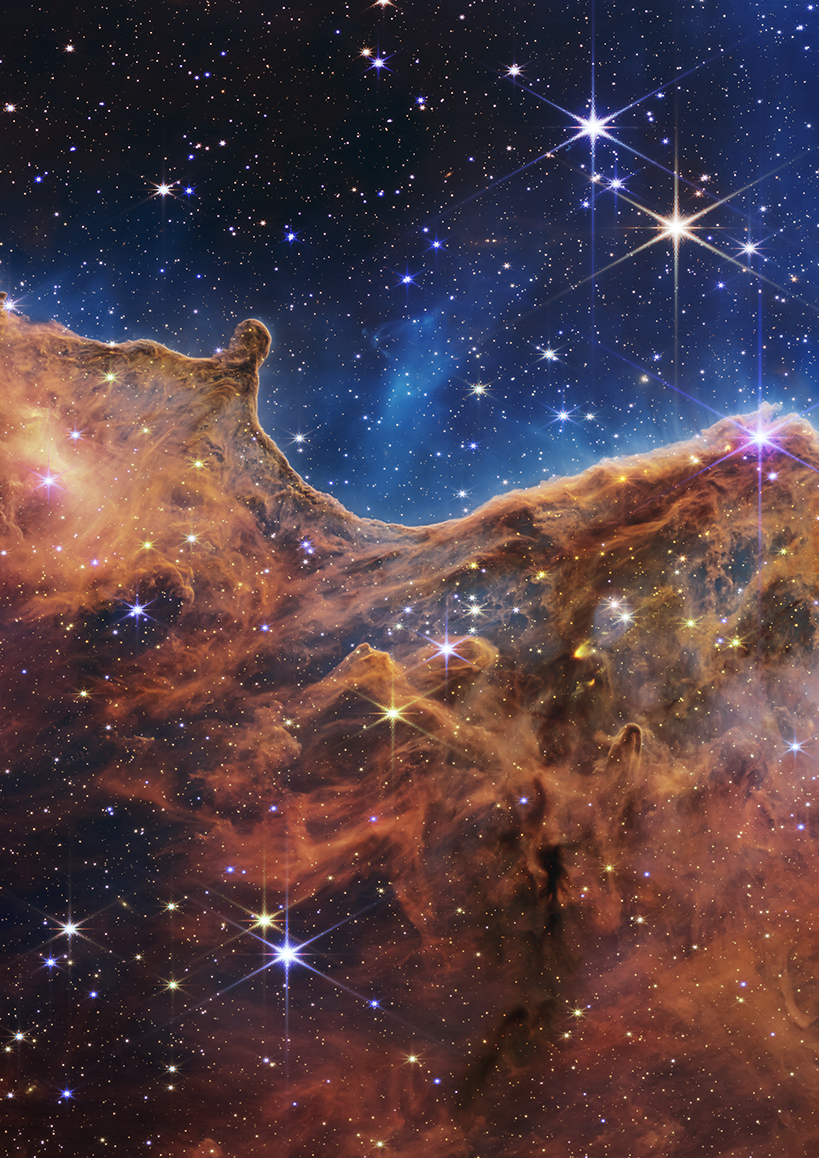
\includegraphics[width=\paperwidth]{Images/Carina_nebula_JWST1}}
    }
    \BgThispage
    
    \fancyfoot[C]{\color{white}\thepage}
    \fancyfoot[L]{\vspace{3.5ex}\tiny\textcolor{white}{Credit: NASA, ESA, CSA, STScI}}
    \clearpage
    \newpage
    
    \renewcommand{\CurrentTitleColor}{\color{white}}
\fi

\chapter{Conclusions and outlook}
\label{ch:Conclusions_and_outlook}

\ifsetDraft
\else
    \renewcommand{\CurrentTitleColor}{\color{black}}
    
%    \vspace*{\fill}
%    \setlength{\epigraphwidth}{0.6\textwidth}
%    {\color{white} \epigraph{\textit{The Road goes ever on and on\\
%                \hspace{2ex} Down from the door where it began.\\
%                Now far ahead the Road has gone,\\
%                \hspace{2ex} And I must follow, if I can,\\
%                Pursuing it with eager feet,\\
%                \hspace{2ex} Until it joins some larger way\\
%                Where many paths and errands meet.\\
%                \hspace{2ex} And whither then? I cannot say.}}{--- J.R.R. Tolkien, The Fellowship of the Ring (1954)}}
%    \vspace*{\fill}
    
    \backgroundsetup{
        scale=1,
        color=black,
        opacity=1,
        placement=top,
        angle=0,
        contents={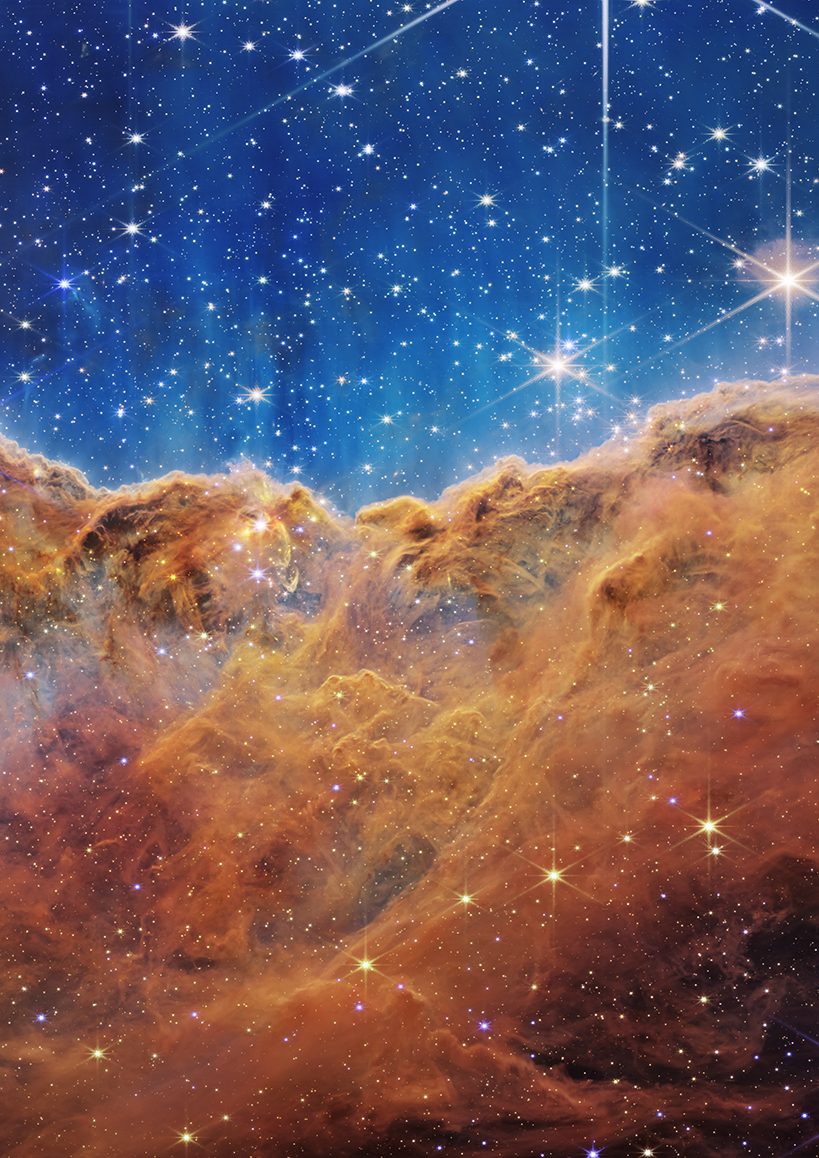
\includegraphics[width=\paperwidth]{Images/Carina_nebula_JWST2}}
    }
    \BgThispage
    
    \fancyhf{}
    \fancyfoot[C]{\color{white}\thepage}
    \newpage
    \setFancyHdr
\fi

\lettrine{I}{n the previous chapters}, I have discussed the properties of star-forming galaxies and the intergalactic medium in the early Universe. In this chapter, I briefly identify the main findings and potential directions of future investigations concerning the topics discussed.

\section{Conclusions}
\label{chCsec:Conclusions}

The main themes of this thesis revolve around galaxies in the early Universe and their large-scale environment, the cosmic web. In \cref{ch:Prospects_for_observing_the_low-density_cosmic_web_in_Lya_emission}, we discussed the potential of the \lya\ line to observe the diffuse, low-density IGM. Although challenging, the current and certainly the next generation of telescopes should be able to begin probing this largely unexplored territory in the post-reionisation Universe, complementary to 21-cm studies of neutral hydrogen in the dark ages and at cosmic dawn.

Meanwhile, the last decade has seen \textit{HST} extend the high-redshift galaxy frontier by identifying significant samples of galaxies in the very early Universe, towards the end of, and indeed in the heart of, the reionisation epoch. At the same time, ground-based spectrographs have been pushed to their limits to spectroscopically follow up these intrinsically faint distant galaxies, as exemplified in \cref{ch:Assessing_the_sources_of_reionisation}. In this chapter, we conducted a case study of what we expect might be a typical EoR galaxy, in preparation for the NIR spectroscopy of galaxies well and truly inside the EoR that will be undertaken by \textit{JWST}. We explored several promising emission-line diagnostics, finding tentative evidence for LyC escape and a departure from the FMR. Though this is in line with expectations for a young, metal-poor galaxy, we still lack convincing evidence that these effects are commonplace among EoR galaxies due to the observational challenges faced in spectroscopy of high-redshift galaxies, many of which however may soon be overcome by \textit{JWST} (see \cref{chCssec:JWST}).

\Cref{ch:Dual_constraints_with_ALMA} discussed how ALMA has proven to be a critical tool for studying the ISM properties of high-redshift galaxies in the FIR regime. As expected, these systems appear to have young stellar populations and hard radiation fields. However, somewhat surprisingly, we also found indications that some of these galaxies may have already reached quite advanced evolutionary stages, having already built up significant amounts of metals and dust.

Naturally, a lot of open questions still remain in spite of -- but in many cases also provoked by -- the findings of spectroscopic studies that have been performed to date by the astronomical community focussing on the early Universe. In the next section, I will discuss some of the potential avenues for the continuation of the research presented in this thesis in light of two of the main facilities expected to be at the cutting edge of high-redshift extragalactic science over the next few years, \textit{JWST} and ALMA.

\section{Outlook}
\label{chCsec:Outlook}

\subsection{Prospects for extragalactic science with \textit{JWST}}
\label{chCssec:JWST}

In \cref{ch:Assessing_the_sources_of_reionisation,ch:Dual_constraints_with_ALMA}, I have discussed how spectroscopic measurements of high-redshift galaxies are starting to characterise the process of star formation in the early Universe and its contribution to Cosmic Reionisation. Importantly, the recent commissioning of \textit{JWST} \citep{2006SSRv..123..485G} will enable detailed rest-frame UV and optical spectroscopic (and photometric) measurements in statistically meaningful samples of EoR galaxies. In the following, I briefly describe the capabilities of the four different instruments on board \textit{JWST} and their observing modes relevant to the topics covered here.

Already briefly discussed in \cref{ch:Assessing_the_sources_of_reionisation}, NIRSpec \citep{2022A&A...661A..80J, 2022A&A...661A..81F} is capable of multi-object, fixed-slit, and IFU spectroscopy in the NIR regime ($0.6$-$5.3 \, \mathrm{\upmu m}$) at three different spectral resolution modes: low ($R \approx 100$), medium ($R \approx 1000$), and ``high'' ($R \approx 2700$) resolution. The Near-Infrared Camera \citep[NIRCam;][]{2005SPIE.5904....1R, 2012SPIE.8442E..2NB} contains two nearly identical modules covering adjacent fields of view and operates in approximately the same wavelength regime as NIRSpec ($0.6$-$5 \, \mathrm{\upmu m}$). A dichroid allows both modules to simultaneously image the same field in a short-wavelength ($0.6$-$2.3 \, \mathrm{\upmu m}$) and long-wavelength ($2.4$-$5 \, \mathrm{\upmu m}$) channel, the latter of which is also used to perform wide-field slitless spectroscopy at medium resolution ($R \approx 1400$). The Near-Infrared Imager and Slitless Spectrograph \citep[NIRISS;][]{2012SPIE.8442E..2RD} provides complementary wide-field slitless spectroscopy at short wavelengths ($0.8$-$2.2 \, \mathrm{\upmu m}$) as well as NIR imaging ($0.8$-$5 \, \mathrm{\upmu m}$). Finally, the Mid-Infrared Instrument \citep[MIRI;][]{2015PASP..127..584R} has an imaging mode with a number of broadband MIR filters ($4.9$-$28.8 \, \mathrm{\upmu m}$), but it is also capable of low-resolution ($R \approx 100$) fixed-slit spectroscopy and medium-resolution ($R \approx 2500$) IFU spectroscopy.

One of the main deep, extragalactic surveys that \textit{JWST} will carry out is JADES, the \textit{JWST} Advanced Extragalactic Survey \citep[e.g.][]{2018ApJS..236...33W}, exploiting the combined capabilities of the NIRSpec and NIRCam instruments. The wealth of spectroscopic data it will obtain as a follow-up of high-redshift targets identified in photometric data taken by \textit{HST}, and \textit{JWST}/NIRCam in the second stage of the survey, will allow a wide range of science goals relating to galaxies in the early Universe to be explored.

First of all, the imaging from NIRCam (and MIRI, if available), combined with the low-resolution NIRSpec spectra, will probe the stellar continuum not only of the young, but also older stellar populations (cf. \cref{chIsssec:Counting_stars,chIssec:Stellar_continuum}), thereby significantly improving the accuracy of stellar mass estimates compared to current constraints derived from shorter wavelengths that are dominated by young stellar light \citep[e.g.][]{2022arXiv220803281T}. Concerning the spectroscopy specifically, JADES is expected to detect a significant number of high-redshift ($z \gtrsim 6$) \lya\ emitters, whose prevalence as a function of redshift, owing to the effect of IGM absorption discussed in \cref{chIsssec:Cosmic_Reionisation}, can be used to study the cosmic neutral fraction in the later stages of Cosmic Reionisation \citep{2010MNRAS.408.1628S, 2014ApJ...793..113P, 2014MNRAS.443.2831C, 2018ApJ...856....2M, 2019MNRAS.489.2669M, 2022MNRAS.512.5960M}. In combination with rest-frame UV and optical emission lines and continuum, the expected ionising photon production and escape of these systems can be characterised, among many other physical properties. In particular, the low-resolution ($R \approx 100$) mode will be used to study the continuum emission to constrain stellar masses and ages, while the medium-resolution ($R \approx 1000$ and $R \approx 2700$) gratings will deliver spectra suitable for detailed emission-line studies. For instance, the \lya\ line profile can be used to map out the structure of ionised regions carved out by galaxies \citep[``ionised bubbles'';][]{2020MNRAS.499.1395M}. In the absence of \lya\ emission, different diagnostics of LyC escape (such as the $\MgII \, \lambda \, 2796, 2804 \, \Angstrom$ doublet) can be applied to establish a census of star-forming galaxies actively contributing to reionisation. Traditional methods using strong lines in the rest-frame optical (e.g. \Halpha\ and $\OIIIf \, \lambda \, 5008 \, \Angstrom$) can for the first time be applied to EoR galaxies to measure SFRs and metallicities (cf. \cref{chIssec:Chemical_enrichment}), characterise AGN activity (\cref{chIssec:Nebular_emission_and_emission-line_diagnostics}), and study the kinematics (using the higher-resolution mode, $R \approx 2700$).

\subsection{Prospects for extragalactic science with ALMA}
\label{chCssec:ALMA}

As emphasised in \cref{ch:Dual_constraints_with_ALMA}, the presence of dust in EoR galaxies may be significant. The dust properties, however, are still largely unconstrained: in particular, the uncertainty in the dust temperature has a large impact on many derived physical properties such as the dust mass and obscured SFR (\cref{chDsec:Discussion:Dust_properties}). Therefore, it is crucial to study the FIR SED at multiple wavelengths and begin to establish the typical dust properties of EoR galaxies. Preliminary efforts using the \program{mercurius} code to empirically constrain the greybody parameters of all high-redshift galaxies with multi-band dust-continuum detections point out that while some galaxies host substantial dust reservoirs -- perhaps more than would be expected as a result of SN activity alone -- there does not seem to be a strong redshift evolution in the dust emissivity \citetext{Witstok et al., in prep.}.

In addition, to better understand the emergence of these dust reservoirs, we have an approved ALMA program in Cycle 9 (2022.1.00925.S; PI: Witstok) that will constrain the dust properties of COS-3018555981 (discussed in detail in \cref{chDsec:Discussion:Dust_properties}) with observations in bands 5, 7, and 8. With several dust-continuum detections, we can infer a first estimate of the shape of its FIR SED which will allow us to more accurately measure the greybody parameters (i.e. dust temperature, mass, and emissivity). As shown in \cref{ch:Dual_constraints_with_ALMA}, this will potentially reveal the existence of cold, massive dust reservoir in the very early Universe, in stark contrast to what may be expected of typical young star-forming galaxies at this era \citep{2022MNRAS.513.3122S, 2022MNRAS.tmpL..72V}. Although it will merely be a singular, perhaps extreme example, such a detailed dissection of the dust emission of a normal star-forming galaxy in the EoR is a crucial first step towards the characterisation of dust properties at high redshift.

It is uncertain what surprises will be revealed in relation to the emergence of the first galaxies in the coming years by ALMA, \textit{JWST}, and other facilities. Above all, however, it is clear that the outlook for extragalactic astronomy is exceptionally bright.

%%!TEX root = ../thesis.tex
% ************************** Thesis Acknowledgements **************************

\begin{acknowledgements}      
    
    First of all, I would like to acknowledge the Institute of Astronomy for having made possible this research. Also, my gratitude goes out to the the developers of all software packages used for this research:
    \begin{enumerate}[label=--]
        \item \program{python}, and its packages: the \program{SciPy} library \citep{Jones2001}, \program{NumPy} \citep{2011CSE....13b..22V}, \program{Matplotlib} \citep{Hunter2007}, and \program{Astropy} \citep{2013A&A...558A..33A, 2018AJ....156..123A}.
        \item \program{SAOImage DS9} and \program{TOPCAT} (Tool for OPerations on Catalogues And Tables)
        \item The LaTeX distribution (CITE) %\LaTeX\
    \end{enumerate}
    
    %\noindent
    \par Special thanks goes to Ewald, Girish, and Martin for all their assistance, useful advice, and enlightening discussions.
    
\end{acknowledgements}




% ********************************** Back Matter *******************************
% Backmatter should be commented out, if you are using appendices after References
%\backmatter

% ********************************** Bibliography ******************************
%\begin{spacing}{0.5}

% To use the conventional natbib style referencing
% Bibliography style previews: http://nodonn.tipido.net/bibstyle.php
% Reference styles: http://sites.stat.psu.edu/~surajit/present/bib.htm

%\bibliographystyle{apalike}
\bibliographystyle{mnras}
%\bibliographystyle{unsrt} % Use for unsorted references  
%\bibliographystyle{plainnat} % use this to have URLs listed in References
\cleardoublepage
\bibliography{References/references} % Path to your References.bib file

% If you would like to use BibLaTeX for your references, pass `custombib' as
% an option in the document class. The location of 'reference.bib' should be
% specified in the preamble.tex file in the custombib section.
% Comment out the lines related to natbib above and uncomment the following line.

%\printbibliography[heading=bibintoc, title={References}]


%\end{spacing}

% ********************************** Appendices ********************************

\begin{appendices} % Using appendices environment for more functionality
	% Use input if you want "Appendices" in TOC (option 'toc' for package appendix)
	%!TEX root = ../thesis.tex
% ******************************* Thesis Appendix A ****************************
\chapter{Modelling \texorpdfstring{\lymana}{\lymanatext} emission}
\label{app:Modelling Lya emission}

%\renewcommand\thesection{A.\arabic{section}}
%\setcounter{section}{0}

%\renewcommand\thefigure{A.\arabic{figure}}
%\setcounter{figure}{0}

\section{Model parameters and fitting functions}
\label{appPsec:Model parameters}

\subsection{Emission processes}

This section contains the fitting functions for the relevant quantities in the formulae for recombination and collisional excitation emissivity (\cref{chPeq:Recombination emissivity,chPeq:Collisional excitation emissivity} in \cref{chPssec:Lya recombination emission,chPssec:Lya collisional excitation emission}), which are repeated here for clarity. Recombination emissivity (\cref{chPeq:Recombination emissivity}) is written as
\begin{equation}
    \label{appPeq:AppRecombination emissivity}
    \epsilon_\text{rec}(T) = f_\text{rec, A/B} (T) \, n_\text{e} \, n_\text{\ion{H}{II}} \, \alpha_\text{A/B}(T) \, E_\text{\lya} \, .
\end{equation}

Collisional excitation emissivity (\cref{chPeq:Collisional excitation emissivity}) is given by
\begin{equation}
    \label{appPeq:AppCollisional excitation emissivity}
    \epsilon_\text{exc}(T) = \gamma_\text{1s2p} (T) \, n_\text{e} \, n_\text{\ion{H}{I}} \, E_\text{\lya} \, .
\end{equation}

\subsubsection{Recombination fitting functions}

The underlying equation governing \lya\ emission due to recombination in the IGM is given in \cref{appPeq:AppRecombination emissivity}. The recombination fraction $f_\text{rec, A/B}$ gives the number of recombinations that ultimately result in the emission of a \lya\ photon. This fraction can be modelled using the relations given in \citet{2008ApJ...672...48C} and \citet{2014PASA...31...40D} and can be summarised as follows:
\begin{equation*}
    f_\text{rec, A/B} = \left\{
    \begin{array}{r}
        \multicolumn{1}{l}{0.41 - 0.165 \log_{10} \left( \frac{T}{10^4 \, \mathrm{K}} \right)} \\
        
        \qquad \qquad \qquad - 0.015 \left( \frac{T}{10^4 \, \mathrm{K}} \right)^{-0.44}, \, \text{case-A} \\
        
        \multicolumn{1}{l}{0.686 - 0.106 \log_{10} \left( \frac{T}{10^4 \, \mathrm{K}} \right)} \\
        
        \qquad \qquad \qquad - 0.009 \left( \frac{T}{10^4 \, \mathrm{K}} \right)^{-0.44}, \, \text{case-B.} \\
    \end{array}
    \right.
\end{equation*}

The recombination coefficient, $\alpha_\text{A/B}$, is given in the work of \citet{2011piim.book.....D} as follows:
\begin{equation*}
    \alpha_\text{A/B} = \left\{
    \begin{array}{r}
        \multicolumn{1}{l}{4.13 \cdot 10^{-13} \left( \frac{T}{10^4 \, \mathrm{K}} \right)^{-0.7131-0.0115 \ln \left( \frac{T}{10^4 \, \mathrm{K}} \right)} \, \mathrm{cm^{3} \, s^{-1}},} \\
        
        \text{case-A} \\
        
        \multicolumn{1}{l}{2.54 \cdot 10^{-13} \left( \frac{T}{10^4 \, \mathrm{K}} \right)^{-0.8163-0.0208 \ln \left( \frac{T}{10^4 \, \mathrm{K}} \right)} \, \mathrm{cm^{3} \, s^{-1}},} \\
        
        \text{case-B.} \\
    \end{array}
    \right.
\end{equation*}

\subsubsection{Collisional excitation fitting functions}

For collisional excitation, the \lya\ luminosity density is given by \cref{appPeq:AppCollisional excitation emissivity}. The function $\gamma_\text{1s2p}$ in this formula is given by
\begin{equation}
    \gamma_\text{1s2p} (T) = \Gamma(T) \exp \left( -\frac{E_\text{\lya}}{k_\text{B}T} \right) \, ,
\end{equation}

\noindent where $k_\text{B}$ is the Boltzmann constant. The function $\Gamma(T)$ is characterised in \citet{1990MNRAS.242..692S} and \citet{1991ApJ...380..302S} as follows:
\begin{equation}
    \label{appPeq:Gamma}
    \Gamma (T) = \exp \left( \sum_{i=0}^{5} c_i \left( \ln T \right)^i \right) \, ,
\end{equation}

\noindent where the coefficients $c_i$ found by \citet{1990MNRAS.242..692S} and \citet{1991ApJ...380..302S} are dependent on the temperature regime (shown in \cref{appPtab:Coefficients}). As noted in \cref{chPsssec:Collisional excitation emissivity}, the rates are not identical to those applied in the cosmological hydrodynamical simulation, but in the relevant temperature regime deviate so little that the \lya\ emission would not be appreciably changed.
\begin{table}
    \centering
    \caption[Coefficients $c_i$ in \cref{appPeq:Gamma}]{
        Coefficients $c_i$ in \cref{appPeq:Gamma} and their corresponding temperature regimes.
    }
    \begin{tabular}{c c l l l}
        
        & & \textbf{Regime 1}   & \textbf{Regime 2}     & \textbf{Regime 3} \\
        
        $c_0$ & & $-1.630155 \cdot 10^{2}$      & $5.279996 \cdot 10^{2}$ & $-2.8133632 \cdot 10^{3}$ \\
        
        $c_1$ & & $8.795711 \cdot 10^{1}$       & $-1.939399 \cdot 10^{2}$ & $8.1509685 \cdot 10^{2}$ \\
        
        $c_2$ & & $-2.057117 \cdot 10^{1}$      & $2.718982 \cdot 10^{1}$ & $-9.4418414 \cdot 10^{1}$ \\
        
        $c_3$ & & $2.359573$                            & $-1.883399$                           & $5.4280565$ \\
        
        $c_4$ & & $-1.339059 \cdot 10^{-1}$     & $6.462462 \cdot 10^{-2}$        & $-1.5467120 \cdot 10^{-1}$ \\
        
        $c_5$ & & $3.021507 \cdot 10^{-3}$      & $-8.811076 \cdot 10^{-4}$        & $1.7439112 \cdot 10^{-3}$ \\
    \end{tabular}
    
    \vspace{0.5ex}
    
    \begin{tabular}{c c}
        
        \textbf{Regimes}        & \textbf{Temperature values} \\
        
        Regime 1        & $2 \cdot 10^3 \, \mathrm{K} \leq T < 6 \cdot 10^4 \, \mathrm{K}$ \\
        
        Regime 2        & $6 \cdot 10^4 \, \mathrm{K} \leq T < 6 \cdot 10^6 \, \mathrm{K}$ \\
        
        Regime 3        & $6 \cdot 10^6 \, \mathrm{K} \leq T \leq 1 \cdot 10^8 \, \mathrm{K}$ \\
    \end{tabular}
    \label{appPtab:Coefficients}
\end{table}

\begin{figure}
    \centering
    \includegraphics[width=\columnwidth]{"Plots/ChapterP/Optical_depths"}
    \caption[2D histogram of \lya\ optical depth $\tau$ and overdensity $\rho/\bar{\rho}$ at $z=4.8$]{Two-dimensional density histogram for each of $2048$ pixels in spectra along $5000$ (randomly selected) lines of sight at $z=4.8$, as a function of the \lya\ optical depth $\tau$ and overdensity $\rho/\bar{\rho}$ in the sightline; the two parameters are measured at line centre, where the optical depth was divided by $2$ just to account for the hydrogen between the source and the observer (see text).}
    \label{appPfig:2D scatter}
\end{figure}
\begin{figure*}
    \centering
    \includegraphics[width=\linewidth]{"Plots/ChapterP/Column_density"}
    \caption[Observed column density at $z=4.8$]
    {Simulated column density of neutral hydrogen, $N_\text{\ion{H}{I}}$, in a simulation snapshot at $z=4.8$. The same regions as in \cref{chPfig:4nsobs_ov} are shown. Moreover, the same density thresholds used for the collisional excitation component are applied, that is only gas below half the critical self-shielding density is shown, meaning this is the column density that would correspond to a narrowband image of the low-density gas with $\Delta \lambda_\text{obs} = 3.75 \, \Angstrom$ ($\ssim 1.19 \, h^{-1} \, \mathrm{cMpc}$). Panel~\textbf{a} shows an overview of part of the simulation snapshot that corresponds to region~1 in \cref{chPfig:SB}. This is centred on the same comoving coordinates both spatially and spectrally, but now less extended in wavelength range. This panel shows a region of $8 \times 8 \, h^{-2} \, \mathrm{cMpc}^2$ ($5.2 \times 5.2 \, \mathrm{arcmin}^2$) on a pixel grid of $1024 \times 1024$. Panels~\textbf{b}-\textbf{d} show column density maps of neutral hydrogen the size of the MUSE FOV consisting of $300 \times 300$ pixels. The areas covered by these maps are indicated by the black squares in the overview panel~a. In the bottom left corner of each panel, two different measures of the overdensity of the region are shown (see \cref{chPssec:Simulated observations} for more details). In panels~b-d, halos with halo mass of $M_\mathrm{h} > 10^{9.5} \, \mathrm{M_\odot}$ are shown as circles, their size indicating their projected virial radius (see \cref{chPssec:Simulated observations}). The most massive halo in each panel is annotated.}
    \label{appPfig:NHI}
\end{figure*}
\begin{figure*}
    \centering
    \includegraphics[width=\linewidth]{"Plots/ChapterP/Redshift_SB_evolution"}
    \caption[Observed \lya\ surface brightness at different redshifts]
    {\lya\ SB for a combination of recombination emission (of all gas in the simulation) below the mirror limit and collisional excitation of gas below half the critical self-shielding density at different redshifts. Both the mirror limit and the critical self-shielding density evolve as a function of redshift (see \cref{chPfig:UVB_limits}). The panels show snapshots at redshifts of $z=6.00$, $z=5.58$, $z=4.49$, $z=4.00$, $z=3.60$, $z=3.20$ for a narrowband with $\Delta \lambda_\text{obs} = 3.75 \, \Angstrom$; at $z=5.76$; this corresponds to $\ssim 1.19 \, h^{-1} \, \mathrm{cMpc}$, but this again changes with redshift. The panels all display a pixel grid of $300 \times 300$ and the angular size of the MUSE FOV ($1 \times 1 \, \mathrm{arcmin}^2$), which translates to different physical sizes at each corresponding redshift. The regions are all centred at the same comoving transverse coordinates as panel~d in \cref{chPfig:4nsobs_ov} and \cref{chPfig:4nsobs_ov150}; however, the narrowband centre (the coordinate along the line of sight) has been chosen to coincide with the most massive halo in each panel to ensure the entire filament is captured in each panel. The two numbers in the bottom left corner show the same two different measures of the overdensity of the region, $\Delta_\mathrm{baryon}$ and $\Delta_\mathrm{halo}$ (see \cref{chPsssec:Cosmic variance and narrowband widths} for more details). Halos with halo mass of $M_\mathrm{h} > 10^{9.5} \, \mathrm{M_\odot}$ are shown as circles, their size indicating their projected virial radius. The most massive halo in each panel is annotated. The scale varies between different panels since the angular size is kept constant across all redshifts.}
    \label{appPfig:4nsobs_mos}
\end{figure*}

\section{\texorpdfstring{\lya}{\lyatext} optical depth}
\label{appPsec:Lya optical depth}

This work does not contain treatment of \lya\ line radiative transfer effects (\cref{chPsssec:Radiative transfer effects}). For our purposes, the treatment without radiative transfer gives us valuable insights into the lower-density IGM filaments on large, cosmological scales without having to resort to implementing computationally expensive radiative transfer methods that are difficult to accurately model, for example because the effects of dust are poorly constrained.

In \cref{appPfig:2D scatter}, a two-dimensional density histogram for each of $2048$ pixels in mock \lya\ absorption spectra along $5000$ lines of sight at $z=4.8$ is shown as a function of both the \lya\ optical depth $\tau$ and overdensity $\rho/\bar{\rho}$ in the relevant pixel. These spectra are extracted on the fly at redshift intervals $\Delta z = 0.1$ and are constructed from the gas density and neutral fraction, temperature, and peculiar velocity of neutral hydrogen along these lines of sight \citep[for details, see][ where they are studied in the context of the \lya\ forest]{2017MNRAS.464..897B}. The peculiar velocity of the gas in a given pixel has been used to translate its position to redshift space where optical depth is determined. Therefore both density and optical depth are effectively measured at line centre. The optical depth was divided by a factor of $2$ to account for the fact that on average only half of the matter is in between the source and the observer; the other half is located behind the source.\footnote{We note that the division by $2$ is necessary as the \lya\ optical depths were originally extracted to study \lya\ forest absorption in the spectra of background sources in which case all the gas that affects a pixel in redshift space is in front of the source in real space.} From this figure, it is clear that at mean density optical depths of order $10$ are reached, indicating that radiative transfer has an effect on most regions. However, effectively this plot still shows an overestimated measure of optical depth. Since it uses a measure of optical depth at line centre, this does not mean that physically no \lya\ emission is detected in the optically thick regime ($\tau > 1$). Many \lya\ photons may be able to escape because an initial scattering not only changes the direction of propagation of photons, but also shifts their frequency and the optical depth decreases quickly when moving away from line centre. An example of this effect is the \lya\ radiation from galaxies, where densities are high enough to have optical depths of the order of $10^6$, but escape away from line centre is still possible. The optical depth thus mostly informs the expected degree of scattering, that is spatial and spectral broadening of the line profile.

Additionally, the neutral hydrogen (\ion{H}{I}) column density at $z=4.8$ is shown in \cref{appPfig:NHI} for precisely the same simulation region (and density limits used for collisional excitation) as in \cref{chPfig:4nsobs_ov}, with the same narrowband width of $\Delta \lambda_\text{obs} = 3.75 \, \Angstrom$ (equivalent to $\ssim 1.19 \, h^{-1} \, \mathrm{cMpc}$), and pixel grids of pixel grid of $1024 \times 1024$ (panel~a) and $300 \times 300$ (panels~b-d). The overview map (panel~a) shows that all areas have column densities of at least $N_\text{\ion{H}{I}} \sim 10^{15} \, \mathrm{cm^{-2}}$. The most extreme features of the low-density gas show column densities of $10^{17}$-$10^{18} \, \mathrm{cm^{-2}}$, which is the range of Lyman-limit systems. Except for the self-shielding prescription, simulations that are very similar to that used in this work are found to match observational \ion{H}{I} column density distributions well at lower redshifts, where data are more abundant, at least up to $N_\text{\ion{H}{I}} \sim 3 \cdot 10^{16} \, \mathrm{cm^{-2}}$, where self-shielding is expected to have a negligible effect \citep{2017MNRAS.464..897B}. At higher column densities, the self-shielding prescription that we use \citep{2013MNRAS.430.2427R} was calibrated to yield realistic column density distributions. At the highest column densities, our simulation will certainly be affected by our simplistic galaxy formation model. These high densities are, however, not the focus of this study.

As with \cref{appPfig:2D scatter}, it has to be taken into account that this is the column density projected for the entire narrowband. Emitting structures seen within this slice always lie between the boundaries of this region. Therefore part of the column density that is projected may be behind the emitting region, as seen from the observer's perspective. This means that, on average, the actual values of column densities photons travels through is about half of what is displayed.

As discussed in \cref{chPsssec:Radiative transfer effects}, it is expected that the precise way in which these scattering processes affect the perceived SB images are the result of a competition between two underlying effects. One possibility is that the photons emerging from the filamentary structure might be spread out, causing the signal to become fainter. The second possibility is that the filament signal might be enhanced by \lya\ radiation coming from nearby dense structures (where additional radiation is likely to be produced in galaxies) that is scattered in the filament, thereby causing the filaments to appear brighter. As mentioned, similar simulations including radiative transfer show a mixture of these two effects, where the SB of filaments generally is not affected much or even boosted \citetext{private communication, Weinberger, 2019}.

\section{Redshift evolution}
\label{appPsec:Redshift evolution}

The region extensively discussed in \cref{chPssec:Simulated observations}, shown in panel~d of \cref{chPfig:4nsobs_ov} and all panels in \cref{chPfig:4nsobs_ov150}, is shown at different redshifts in \cref{appPfig:4nsobs_mos}, again showing the combination of recombination emission of all gas in the simulation below the mirror limit and collisional excitation of gas below half the critical self-shielding density. The panels shown are centred at the same transverse comoving coordinates as panel~d in \cref{chPfig:4nsobs_ov} and all panels in \cref{chPfig:4nsobs_ov150}, but the narrowband centre (the coordinate along the line of sight) is now chosen to coincide with the most massive halo in each panel to ensure the same structure is captured in each panel. Each panel covers the angular size of the MUSE FOV, the physical extent of which varies at different redshifts.

Following the redshift evolution from high to low (going from panel~a to panel~f), we note that the comoving size of the observed region shrinks roughly from $\ssim 1.5 \times 1.5 \, h^{-2} \, \mathrm{cMpc}^2$ to just over $\ssim 1 \times 1 \, h^{-2} \, \mathrm{cMpc}^2$ since the angular size of the FOV is kept fixed at $1 \times 1 \, \mathrm{arcmin}^2$. The appearance of new massive ($M_\mathrm{h} > 10^{9.5} \, \mathrm{M_\odot}$) halos and their evolution in relative movement and mass accretion, indicated by the increase in their virial radii, can also be traced between the different panels. Panel~e, at $z=3.60$, has the same redshift as shown in the bottom two panels of \cref{chPfig:4nsobs_ov150}.

With these conservative limits that exclude emission from the dense (and complicated) central regions of halos, \lya\ emission appears brighter at low redshift, where the mirror limit is less affected by SB dimming and self-shielding effects only start to play a role at higher overdensities, as discussed in \cref{chPsssec:Sensitivity analysis}. Panels~a and b appear particularly homogeneous as large portions are impacted by the mirror limit ($24.6\%$ and $22.1\%$ of pixels exceeding the mirror limit). We note that at low redshift, on the other hand, there is less low-density gas that is luminous in \lya, especially within the large, central halo. The gas there is likely denser and hotter and thus less effective at emitting \lya\ radiation, at least within the low-density regime that we are considering (cf. \cref{chPfig:z_evolution_lum,fig:Luminosity phase space} and their discussion in the text).
	%!TEX root = ../thesis.tex
% ******************************* Thesis Appendix C ****************************
\chapter{Assessing the sources of reionisation}
\label{app:Assessing the sources of reionisation}

%\renewcommand\thesection{A.\arabic{section}}
%\setcounter{section}{0}

%\renewcommand\thefigure{A.\arabic{figure}}
%\setcounter{figure}{0}

\section{\texorpdfstring{\MgII}{MgII} and \texorpdfstring{\CIII}{CIII} significance}
\label{appAsec:MgII and CIII significance}

\begin{table}
    \centering
    \caption[Significance of the \MgII\ detection]
    {Measured velocity offset and line flux in different subsets of the X-shooter data, corresponding to the rows in \cref{appAfig:MgII significance}. Given quantities are defined as in \cref{chAtab:Results}.
    }
    \begin{tabular}{lcc}
        \hline
        Configuration & $\Delta v \, (\mathrm{km/s})$ & $\mathrm{Flux} \, (10^{-18} \, \mathrm{erg \, s^{-1} \, cm^{-2}})$
        \\
        \hline
        \csvreader[separator=pipe, late after line=\\, head to column names]{Tables/ChapterA/MgII_appendix.csv}{}{\ptype & \ifcsvstrcmp{\dv}{nan}{\dots}{$\dv \ifcsvstrcmp{\dverr}{nan}{}{\pm \dverr}$} & \ifcsvstrcmp{\flux}{nan}{\dots}{\ifcsvstrcmp{\uplim}{True}{$<\flux$}{$\flux \pm \fluxerr$}}
        }
    \end{tabular}
    \label{appAtab:MgII significance}
\end{table}

\begin{figure*}
    \centering
    \includegraphics[width=\linewidth]{"Plots/ChapterA/MgII_significance"}
    \caption[Various X-shooter spectra of \MgII]{X-shooter spectra of \MgII\ for each of the three OBs individually (first three columns) and the combined spectra for a smaller and extended aperture (final two columns). One-dimensional spectra for the individual OBs have been extracted from the same smaller aperture as in the fourth column.
    }
    \label{appAfig:MgII significance}
\end{figure*}

In this appendix, we elaborate on the significance of the (non-)detections of the \MgII\ emission line and the $\CIIIs \, \lambda \, 1907 \, \Angstrom, \CIIIf \, \lambda \, 1909 \, \Angstrom$ doublet. In \cref{appAfig:MgII significance}, X-shooter spectra of \MgII\ are shown for each of the three observation blocks (OBs) individually (first three columns) and the combined result for a smaller and extended aperture (final two columns). The measured velocity offset and flux for each different configuration are summarised in \cref{appAtab:MgII significance}.

Furthermore, \cref{appAfig:CIII non-detection} shows the portion of the spectrum where the \CIII\ doublet would be expected, both without and with telluric absorption correction (TAC; see \cref{chAssec:Observations: X-shooter}). It is unclear whether a signal is present in the spectra, which lack a clear dark-light-dark pattern (cf. \cref{chAfig:Overview panel}), in part because of skyline contamination and partly owing to the strong telluric absorption. We have chosen not to attempt to measure an upper limit for the $\CIIIf \, \lambda \, 1909 \, \Angstrom$ line directly, as it falls precisely on a region that is heavily impacted by skylines and telluric absorption. Instead, we assume a line ratio (see \cref{chAssec:Results: X-shooter}).

\begin{figure}
    \centering
    \includegraphics[width=0.6\linewidth]{"Plots/ChapterA/CIII_nondetection"}
    \caption[Non-detections of \CIII]{X-shooter spectra in the wavelength region where the \CIII\ doublet would be expected, both without and with TAC (see \cref{chAssec:Observations: X-shooter}). The top row shows the resulting atmospheric transmission calculated by \program{molecfit}. A region within $-200 \,\mathrm{km/s} < v < 200 \, \mathrm{km/s}$ of the expected $1907 \, \Angstrom$ line centre, which has been used to place an upper limit on the flux, is highlighted in the bottom row of one-dimensional spectra.
    }
    \label{appAfig:CIII non-detection}
\end{figure}

\section{SDSS selection}
\label{appAsec:SDSS selection}

For the comparison sample drawn from the SDSS DR7 (discussed in \cref{chAssec:Discussion: NeIII/OII}), we outline the selection criteria here in detail. Following previous studies \citep[e.g.][]{2006MNRAS.372..961K, 2014ApJ...788...88J, 2016MNRAS.456.3354F}, we select galaxies satisfying the following criteria:
\begin{enumerate}[label=(\roman*)]
    \item $\mathtt{TARGETTYPE} = \mathrm{GALAXY}$ and $\mathtt{Z\_WARNING} = 0$.
    \item For all emission lines in the ratios \OIIIf/\Hbeta, \NII/\Halpha, \SII/\Halpha, and \OI/\Halpha\ used in \citetalias{1981PASP...93....5B} diagrams, we require a SNR of $\text{SNR} > 3/\sqrt{2} \approx 2.12$ on the ratios themselves (leading to a more complete sample, see \citet{2014ApJ...788...88J} -- additionally, formal uncertainty corrections as discussed in their Appendix A have been applied). Furthermore, we only select galaxies with $\text{SNR} > 30$ on the \OII\ doublet -- see the discussion in \cref{chAssec:Discussion: NeIII/OII}.
    \item In order to align with previous studies, redshifts between $0.04 < z < 0.2$. These lower and upper limits are imposed to avoid strong fiber-aperture effects, and to cover detections of intrinsically weak lines while maintaining a good completeness for Seyfert-type galaxies, respectively \citep[e.g.][]{2014ApJ...788...88J}.
    \item A valid stellar mass measurement ($17$ entries have $M_* = -1$).
\end{enumerate}
This leads to a final sample of $8960$ galaxies. We classify the galaxies into star-forming, composite, Seyfert, and LINER classes (although we will focus only on star-forming and Seyfert types), based on the \NII, \SII, and \OI\ \citetalias{1981PASP...93....5B} diagrams, following \citet{2006MNRAS.372..961K}. Subsequently, the line fluxes are corrected for dust extinction using the \citet{1989ApJ...345..245C} reddening curve assuming $R_V = A_V/E(B-V) = 3.1$, and a fiducial intrinsic \Halpha/\Hbeta\ ratio of $2.85$ for star-forming galaxies, and $3.1$ for AGN-dominated systems \citep[for case-B recombination at $T = 10^4 \, \mathrm{K}$ and $n_e \sim 10^2$-$10^4 \, \mathrm{cm^{-3}}$, see][]{2006MNRAS.372..961K}. In this sample, $2484$ galaxies or 27.7\% have a $\text{SNR} > 5$ \NeIII\ detection.

\section{\textit{JWST} ETC calculation}
\label{appAsec:JWST ETC calculation}

Given the observed $\MgII \, \lambda \, 2796 \, \Angstrom$ flux of $5.0 \cdot 10^{-18} \, \mathrm{erg \, s^{-1} \, cm^{-2}}$ (see \cref{chAtab:Results}) and assuming a typical flux ratio of $F_{2796}/F_{2804} \approx 1.9$ between the $\MgII$ lines at $2796 \, \Angstrom$ and $2804 \, \Angstrom$ \citep[e.g.][]{2018ApJ...855...96H}, the total flux of the doublet would become $7.6 \cdot 10^{-18} \, \mathrm{erg \, s^{-1} \, cm^{-2}}$. However, taking into account the lensing magnification of $\mu = 29$, we derive an intrinsic flux of $2.6 \cdot 10^{-19} \, \mathrm{erg \, s^{-1} \, cm^{-2}}$ at $z=4.88$. We note that the uncertainty and spatial variation of the lensing magnification makes this only a rough estimate of the true intrinsic flux. Assuming an object with the same luminosity at $z = 7$ (in which case \MgII\ would be observed at $\lambda_\text{obs} = 2.24 \, \mathrm{\upmu m}$), this would lead to an observed flux of $1.13 \cdot 10^{-19} \, \mathrm{erg \, s^{-1} \, cm^{-2}}$. The continuum flux density from our fit is $2.29 \cdot 10^{-20} \, \mathrm{erg \, s^{-1} \, cm^{-2} \, \Angstrom^{-1}}$ or $383 \, \mathrm{nJy}$ at $\lambda_\text{obs} = 2.24 \, \mathrm{\upmu m}$, which translates to $2.5 \cdot 10^{-22} \, \mathrm{erg \, s^{-1} \, cm^{-2} \, \Angstrom^{-1}}$ or $4.18 \, \mathrm{nJy}$ if it were unlensed at $z=7$.

Alternatively, our estimate implies $F_{2796} = 7.4 \cdot 10^{-20} \, \mathrm{erg \, s^{-1} \, cm^{-2}}$. This is inconsistent with a recent estimate from \citet{2020MNRAS.498.2554C}, the difference being explained by the fact that their higher flux estimate (by a factor $\ssim 8$) arises from considering a source with a $H$-band magnitude of $25$ (in the F160W filter; this corresponds to $M_\mathrm{UV} \simeq -21.9$ at $z=7$). The unlensed observed magnitude of RCS0224z5 is $\ssim 26.8 \, \mathrm{mag}$, which at $z \simeq 4.88$ translates to $M_\mathrm{UV} \simeq -19.6$. This implies an observed magnitude of $27.4$ at $z=7$ -- a factor $\ssim 9$ fainter than a $25 \, \mathrm{mag}$ source -- and is instead appropriate when considering intrinsically fainter and hence more common sources. In a typical extremely deep field, one would on average expect less than one source at $z \sim 7$ with magnitude $25$, and the order of $N \sim 1$ in a medium-deep field, compared to $N \sim 2$ and $N \gtrsim 70$ respectively for a $m_\text{UV} \sim 27.4 \, \mathrm{mag}$ source (derived from the $z \sim 7$ number counts in the $5 \, \mathrm{arcmin^2}$ XDF and $\ssim 120 \, \mathrm{arcmin^2}$ CANDELS-DEEP fields presented in \citealt{2015ApJ...803...34B}).

Simulations\footnote{\textit{JWST} Exposure Time Calculator: \url{https://jwst.etc.stsci.edu}.} of the near-infrared spectrograph on \textit{JWST} (NIRSpec), point out that for an (intrinsically) relatively faint object like RCS0224z5, detecting \MgII\ spectroscopically would be challenging: for example, a $10 \, \mathrm{ks}$ exposure with the multi-object spectrograph observing mode at low resolution would result in a signal of \MgII\ at the level of $0.65 \sigma$ per spectral pixel (but we note that integrating over the few pixels containing the line could slightly increase the overall SNR). At $R \sim 100$, this would render the doublet (separated by $\ssim 770 \, \mathrm{km/s}$) unresolved as well. The same exposure would yield a SNR of $0.56$ per spectral pixel at medium spectral resolution (the F170LP/G235M grating achieving $R \sim 1000$ at $\lambda_\text{obs} = 2.24 \, \mathrm{\upmu m}$), which would resolve the doublet down to $\ssim 300 \, \mathrm{km/s}$. Finally, a deep ($10 \, \mathrm{h}$) exposure allow a SNR of $0.67$ per spectral pixel at high resolution ($R \sim 2000$ or $\ssim 150 \, \mathrm{km/s}$). Still, for objects with a more intense episode of ongoing star formation (possibly boosting the flux by a factor of a few, up to a factor $\ssim 8$ for a $M_\mathrm{UV} \simeq -21.9$ source as in \citealt{2020MNRAS.498.2554C}, as discussed above), or for lensed objects (like RCS0224z5), observations of \MgII\ would be feasible in deep spectroscopic surveys.
    %!TEX root = ../thesis.tex
% ******************************* Thesis Appendix C ****************************
\chapter{Dual constraints with ALMA}
\label{app:Dual constraints with ALMA}

%\renewcommand\thesection{A.\arabic{section}}
%\setcounter{section}{0}

%\renewcommand\thefigure{A.\arabic{figure}}
%\setcounter{figure}{0}

\section{Dust peak temperature measurements}
\label{appDsec:Dust peak temperature measurements}

Here, we briefly discuss the significance of the SED peak temperature as defined in \cref{chDeq:T_peak} and various measurements and predictions reported in the literature which are included in \cref{chDfig:T_peak_evolution}. Importantly, the peak temperature offers a way to compare observations of the dust temperature consistently since this approach avoids degeneracies introduced by the chosen opacity model, a largely unconstrained quantity that is typically assumed to be a fixed value in the greybody spectrum \citep[e.g.][]{2014PhR...541...45C}.

For a perfect blackbody, the intrinsic temperature $T_\text{dust}$ is exactly equal to the peak temperature but notably, for a greybody $T_\text{peak}$ is generally lower \citep{2012MNRAS.425.3094C}. This effect can be understood by considering a simplistic two-component dust model, where the radiation field is driven towards thermal equilibrium through absorption by the colder component in the optically thick regime, resulting in an observed outward spectrum with a peak wavelength shifted to a higher wavelength (i.e. lower $T_\text{peak}$). Vice versa, when fitting a greybody SED template, the inferred intrinsic dust temperature will strongly depend on the opacity model \citep[e.g.][]{2020A&A...634L..14C}, while the observed peak temperature should remain the same to best fit the observed data. Indeed, $T_\text{peak}$ derived from our fits is approximately unchanged under the assumption of different opacity models, while the inferred $T_\text{dust}$ can change drastically: the more optically thick the SED is (i.e. the higher $\lambda_0$), the higher the resulting intrinsic temperature, $T_\text{dust}$ (see \cref{chDssec:Discussion:Dust_SED_fitting_procedure}).

In \cref{chDfig:T_peak_evolution}, we show the results at lower redshifts ($0 < z < 4$) of \citet{2018A&A...609A..30S}, who fit detailed SED templates built from multiple dust components to stacked spectra. Their reported dust temperatures are thus mass-weighted; however, they find a simple, linear relation where the mass-weighted temperature is roughly $91\%$ of the luminosity-weighted one. This implies temperatures inferred from a greybody, which are necessarily weighted by luminosity, are similar to (although $\ssim 10\%$ higher than) the mass-weighted temperature, effectively setting an upper limit. We also show the (partially extrapolated) linear fit obtained by \citet{2018A&A...609A..30S} and the power-law fit to the peak-temperature evolution of simulated galaxies by \citet{2019MNRAS.489.1397L}.

At intermediate redshifts ($2 < z < 6$), SMGs from the SPT survey \citep{2020ApJ...902...78R} are shown as squares (all other high-redshift galaxies are circles with errorbars). In addition, results for four star-forming galaxies at $z \sim 6$ with photometric detections in three ALMA bands each are included as circles \citep{2020MNRAS.498.4192F}. For five star-forming galaxies at $6 < z < 8$ -- J1211-0118 and J0217-0208 at $z \simeq 6$ \citep{2020ApJ...896...93H}, A1689-zD1 at $z \simeq 7.13$ \citep{2017MNRAS.466..138K, 2020MNRAS.495.1577I, 2021MNRAS.508L..58B}, B14-65666 at $z \simeq 7.15$ \citep{2019PASJ...71...71H, 2021ApJ...923....5S}, and MACS0416-Y1 at $z \simeq 8.31$ \citep{2019ApJ...874...27T, 2020MNRAS.493.4294B} -- we derive dust properties using the same \program{mercurius} fit described in \cref{chDssec:Discussion:Dust_SED_fitting_procedure} for consistency. We allow $\beta_\text{IR}$ to vary freely for A1689-zD1, since there are four dust continuum detections; for MACS0416-Y1, we take $\beta_\text{IR} = 2$ as this provides a better fit. For A1689-zD1 and B14-65666 we opt for the fiducial self-consistent opacity model (we note this assumption has little impact on the inferred $T_\text{peak}$), while for MACS0416-Y1 we use an optically thin SED to obtain a conservative lower limit on the temperature ($95 \%$ confidence). We also adopt an optically thin SED for J1211-0118 and J0217-0208 due to the lack of a size measurement.

\begin{figure*}
    \centering
    \includegraphics[width=\linewidth]{"Plots/ChapterD/Dust_maps_spectra_clean"}
    \caption[Beam placement for spatially resolved analysis.]{Beam placement for spatially resolved analysis. The top row of images shows the UV continuum with contours of the $\ssim 160 \, \mathrm{\upmu m}$ dust continuum (starting from $2 \sigma$ and going up in steps of $1 \sigma$ for COS-2987030247 and UVISTA-Z-019, else $2 \sigma$). The peaks of the UV and dust continua (if detected) are indicated with a black and purple cross, respectively. Contours (at $2 \sigma$ and $3 \sigma$) of the \CIILam\ and \OIIILam\ lines are shown in the second row (and again the UV and dust peaks). The last two rows contain their spectra, both integrated over the entire $2 \sigma$ region (in the same colour as their contours) as well as for the individual regions. For each source, one or several regions are highlighted in the spectra and correspondingly by their number in the second row of images. The filled-in grey region indicates the spectral channels over which the spectra have been integrated.
    }
    \label{appDfig:Beam_placement_for_spatially_resolved_analysis}
\end{figure*}

\section{Spatially resolved analysis}
\label{appDsec:Spatially_resolved_analysis}

In \cref{appDfig:Beam_placement_for_spatially_resolved_analysis}, we show the placements of individual regions (circles with a radius $1.5$ times that of the mean circularised beam between the \CII\ and \OIIIf\ observations) that were used in the spatially resolved analysis (\cref{chDssec:Discussion:OIII/CII_spatially_resolved_analysis}). The \OIIILam\ and \CIILam\ maps were created from imaging parameters that have been chosen to match beam sizes; see \cref{chDtab:Observations1,chDtab:Observations2}; the dust continuum at $\ssim 160 \, \mathrm{\upmu m}$ has the same imaging parameters (and therefore nearly identical beam) as the \CII\ line. IR luminosities were calculated similarly as discussed in \cref{chDsec:Discussion:Dust_properties}. Finally, the UV continuum has been convolved with an effective beam found by the Richardson-Lucy algorithm to match the dust continuum PSF (see also \cref{chDssec:Discussion:OIII/CII_spatially_resolved_analysis}).

For each source, one or several regions are highlighted in the spectra and correspondingly by their number in the second row of images. From the spectra, it for instance becomes clear that, although there still seems to be some residual signal, the \OIIIf\ flux is weakest in region 2 and 5 of COS-3018555981.
\end{appendices}

% *************************************** Index ********************************
%\printthesisindex % If index is present

\end{document}
